\documentclass[twoside]{book}

% Packages required by doxygen
\usepackage{calc}
\usepackage{doxygen}
\usepackage{graphicx}
\usepackage[utf8]{inputenc}
\usepackage{makeidx}
\usepackage{multicol}
\usepackage{multirow}
\usepackage{textcomp}
\usepackage[table]{xcolor}

% Font selection
\usepackage[T1]{fontenc}
\usepackage{mathptmx}
\usepackage[scaled=.90]{helvet}
\usepackage{courier}
\usepackage{amssymb}
\usepackage{sectsty}
\renewcommand{\familydefault}{\sfdefault}
\allsectionsfont{%
  \fontseries{bc}\selectfont%
  \color{darkgray}%
}
\renewcommand{\DoxyLabelFont}{%
  \fontseries{bc}\selectfont%
  \color{darkgray}%
}

% Page & text layout
\usepackage{geometry}
\geometry{%
  a4paper,%
  top=2.5cm,%
  bottom=2.5cm,%
  left=2.5cm,%
  right=2.5cm%
}
\tolerance=750
\hfuzz=15pt
\hbadness=750
\setlength{\emergencystretch}{15pt}
\setlength{\parindent}{0cm}
\setlength{\parskip}{0.2cm}
\makeatletter
\renewcommand{\paragraph}{%
  \@startsection{paragraph}{4}{0ex}{-1.0ex}{1.0ex}{%
    \normalfont\normalsize\bfseries\SS@parafont%
  }%
}
\renewcommand{\subparagraph}{%
  \@startsection{subparagraph}{5}{0ex}{-1.0ex}{1.0ex}{%
    \normalfont\normalsize\bfseries\SS@subparafont%
  }%
}
\makeatother

% Headers & footers
\usepackage{fancyhdr}
\pagestyle{fancyplain}
\fancyhead[LE]{\fancyplain{}{\bfseries\thepage}}
\fancyhead[CE]{\fancyplain{}{}}
\fancyhead[RE]{\fancyplain{}{\bfseries\leftmark}}
\fancyhead[LO]{\fancyplain{}{\bfseries\rightmark}}
\fancyhead[CO]{\fancyplain{}{}}
\fancyhead[RO]{\fancyplain{}{\bfseries\thepage}}
\fancyfoot[LE]{\fancyplain{}{}}
\fancyfoot[CE]{\fancyplain{}{}}
\fancyfoot[RE]{\fancyplain{}{\bfseries\scriptsize Generated on Fri Nov 14 2014 14\-:54\-:11 for Revelator Framework by Doxygen }}
\fancyfoot[LO]{\fancyplain{}{\bfseries\scriptsize Generated on Fri Nov 14 2014 14\-:54\-:11 for Revelator Framework by Doxygen }}
\fancyfoot[CO]{\fancyplain{}{}}
\fancyfoot[RO]{\fancyplain{}{}}
\renewcommand{\footrulewidth}{0.4pt}
\renewcommand{\chaptermark}[1]{%
  \markboth{#1}{}%
}
\renewcommand{\sectionmark}[1]{%
  \markright{\thesection\ #1}%
}

% Indices & bibliography
\usepackage{natbib}
\usepackage[titles]{tocloft}
\setcounter{tocdepth}{3}
\setcounter{secnumdepth}{5}
\makeindex

% Hyperlinks (required, but should be loaded last)
\usepackage{ifpdf}
\ifpdf
  \usepackage[pdftex,pagebackref=true]{hyperref}
\else
  \usepackage[ps2pdf,pagebackref=true]{hyperref}
\fi
\hypersetup{%
  colorlinks=true,%
  linkcolor=blue,%
  citecolor=blue,%
  unicode%
}

% Custom commands
\newcommand{\clearemptydoublepage}{%
  \newpage{\pagestyle{empty}\cleardoublepage}%
}


%===== C O N T E N T S =====

\begin{document}

% Titlepage & ToC
\hypersetup{pageanchor=false}
\pagenumbering{roman}
\begin{titlepage}
\vspace*{7cm}
\begin{center}%
{\Large Revelator Framework }\\
\vspace*{1cm}
{\large Generated by Doxygen 1.8.6}\\
\vspace*{0.5cm}
{\small Fri Nov 14 2014 14:54:11}\\
\end{center}
\end{titlepage}
\clearemptydoublepage
\tableofcontents
\clearemptydoublepage
\pagenumbering{arabic}
\hypersetup{pageanchor=true}

%--- Begin generated contents ---
\chapter{Bug List}
\label{bug}
\hypertarget{bug}{}

\begin{DoxyRefList}
\item[\label{bug__bug000001}%
\hypertarget{bug__bug000001}{}%
Class \hyperlink{class_chunk}{Chunk} ]anything with a vision greater that one chunk next to it is useless. 
\end{DoxyRefList}
\chapter{Hierarchical Index}
\section{Class Hierarchy}
This inheritance list is sorted roughly, but not completely, alphabetically\-:\begin{DoxyCompactList}
\item \contentsline{section}{Audio\-Manager}{\pageref{class_audio_manager}}{}
\item \contentsline{section}{Chunk\-Manager}{\pageref{class_chunk_manager}}{}
\item \contentsline{section}{Collidable}{\pageref{class_collidable}}{}
\begin{DoxyCompactList}
\item \contentsline{section}{Sensor}{\pageref{class_sensor}}{}
\end{DoxyCompactList}
\item \contentsline{section}{Drawable}{\pageref{class_drawable}}{}
\begin{DoxyCompactList}
\item \contentsline{section}{Chunk}{\pageref{class_chunk}}{}
\item \contentsline{section}{Example\-Drawable}{\pageref{class_example_drawable}}{}
\item \contentsline{section}{Game\-Screen}{\pageref{class_game_screen}}{}
\begin{DoxyCompactList}
\item \contentsline{section}{Example\-Test\-Screen}{\pageref{class_example_test_screen}}{}
\end{DoxyCompactList}
\end{DoxyCompactList}
\item \contentsline{section}{Entry\-Object}{\pageref{class_entry_object}}{}
\item \contentsline{section}{Game\-Component}{\pageref{class_game_component}}{}
\begin{DoxyCompactList}
\item \contentsline{section}{Example\-Component}{\pageref{class_example_component}}{}
\item \contentsline{section}{Movable\-Component}{\pageref{class_movable_component}}{}
\end{DoxyCompactList}
\item \contentsline{section}{Game\-Factory}{\pageref{class_game_factory}}{}
\item \contentsline{section}{Game\-Object\-Producer}{\pageref{class_game_object_producer}}{}
\begin{DoxyCompactList}
\item \contentsline{section}{Example\-Component\-Producer}{\pageref{class_example_component_producer}}{}
\item \contentsline{section}{Movable\-Component\-Producer}{\pageref{class_movable_component_producer}}{}
\end{DoxyCompactList}
\item \contentsline{section}{Game\-Screen\-Producer}{\pageref{class_game_screen_producer}}{}
\begin{DoxyCompactList}
\item \contentsline{section}{Example\-Screen\-Producer}{\pageref{class_example_screen_producer}}{}
\end{DoxyCompactList}
\item \contentsline{section}{Keyboard}{\pageref{class_keyboard}}{}
\item \contentsline{section}{Layer}{\pageref{class_layer}}{}
\begin{DoxyCompactList}
\item \contentsline{section}{Example\-Layer}{\pageref{class_example_layer}}{}
\end{DoxyCompactList}
\item \contentsline{section}{Layer\-Producer}{\pageref{class_layer_producer}}{}
\begin{DoxyCompactList}
\item \contentsline{section}{Example\-Layer\-Producer}{\pageref{class_example_layer_producer}}{}
\end{DoxyCompactList}
\item \contentsline{section}{Mouse}{\pageref{class_mouse}}{}
\item \contentsline{section}{Producer\-Package}{\pageref{class_producer_package}}{}
\item \contentsline{section}{Screen\-Manager}{\pageref{class_screen_manager}}{}
\item Sound\begin{DoxyCompactList}
\item \contentsline{section}{S\-F\-X}{\pageref{class_s_f_x}}{}
\end{DoxyCompactList}
\item \contentsline{section}{Spawner}{\pageref{class_spawner}}{}
\item \contentsline{section}{Texture\-Manager}{\pageref{class_texture_manager}}{}
\item \contentsline{section}{Update\-Data}{\pageref{class_update_data}}{}
\item \contentsline{section}{Utils}{\pageref{class_utils}}{}
\item \contentsline{section}{Window\-Manager}{\pageref{class_window_manager}}{}
\end{DoxyCompactList}

\chapter{Class Index}
\section{Class List}
Here are the classes, structs, unions and interfaces with brief descriptions\-:\begin{DoxyCompactList}
\item\contentsline{section}{\hyperlink{class_audio_manager}{Audio\-Manager} \\*This Singleton Manages and plays all music and soundeffects }{\pageref{class_audio_manager}}{}
\item\contentsline{section}{\hyperlink{class_chunk}{Chunk} \\*This Class represents a small portion of a screen }{\pageref{class_chunk}}{}
\item\contentsline{section}{\hyperlink{class_chunk_manager}{Chunk\-Manager} \\*This class contains a reference to the first chunk. and the one the camera hovers above }{\pageref{class_chunk_manager}}{}
\item\contentsline{section}{\hyperlink{class_collidable}{Collidable} \\*This Class holds data used to manage the collision of a gamecomponent }{\pageref{class_collidable}}{}
\item\contentsline{section}{\hyperlink{class_drawable}{Drawable} }{\pageref{class_drawable}}{}
\item\contentsline{section}{\hyperlink{class_entry_object}{Entry\-Object} }{\pageref{class_entry_object}}{}
\item\contentsline{section}{\hyperlink{class_example_component}{Example\-Component} }{\pageref{class_example_component}}{}
\item\contentsline{section}{\hyperlink{class_example_component_producer}{Example\-Component\-Producer} }{\pageref{class_example_component_producer}}{}
\item\contentsline{section}{\hyperlink{class_example_drawable}{Example\-Drawable} }{\pageref{class_example_drawable}}{}
\item\contentsline{section}{\hyperlink{class_example_layer}{Example\-Layer} }{\pageref{class_example_layer}}{}
\item\contentsline{section}{\hyperlink{class_example_layer_producer}{Example\-Layer\-Producer} }{\pageref{class_example_layer_producer}}{}
\item\contentsline{section}{\hyperlink{class_example_screen_producer}{Example\-Screen\-Producer} }{\pageref{class_example_screen_producer}}{}
\item\contentsline{section}{\hyperlink{class_example_test_screen}{Example\-Test\-Screen} }{\pageref{class_example_test_screen}}{}
\item\contentsline{section}{\hyperlink{class_game_component}{Game\-Component} }{\pageref{class_game_component}}{}
\item\contentsline{section}{\hyperlink{class_game_factory}{Game\-Factory} }{\pageref{class_game_factory}}{}
\item\contentsline{section}{\hyperlink{class_game_object_producer}{Game\-Object\-Producer} }{\pageref{class_game_object_producer}}{}
\item\contentsline{section}{\hyperlink{class_game_screen}{Game\-Screen} }{\pageref{class_game_screen}}{}
\item\contentsline{section}{\hyperlink{class_game_screen_producer}{Game\-Screen\-Producer} }{\pageref{class_game_screen_producer}}{}
\item\contentsline{section}{\hyperlink{class_keyboard}{Keyboard} }{\pageref{class_keyboard}}{}
\item\contentsline{section}{\hyperlink{class_layer}{Layer} }{\pageref{class_layer}}{}
\item\contentsline{section}{\hyperlink{class_layer_producer}{Layer\-Producer} }{\pageref{class_layer_producer}}{}
\item\contentsline{section}{\hyperlink{class_mouse}{Mouse} }{\pageref{class_mouse}}{}
\item\contentsline{section}{\hyperlink{class_movable_component}{Movable\-Component} }{\pageref{class_movable_component}}{}
\item\contentsline{section}{\hyperlink{class_movable_component_producer}{Movable\-Component\-Producer} }{\pageref{class_movable_component_producer}}{}
\item\contentsline{section}{\hyperlink{class_producer_package}{Producer\-Package} }{\pageref{class_producer_package}}{}
\item\contentsline{section}{\hyperlink{class_screen_manager}{Screen\-Manager} }{\pageref{class_screen_manager}}{}
\item\contentsline{section}{\hyperlink{class_sensor}{Sensor} }{\pageref{class_sensor}}{}
\item\contentsline{section}{\hyperlink{class_s_f_x}{S\-F\-X} }{\pageref{class_s_f_x}}{}
\item\contentsline{section}{\hyperlink{class_spawner}{Spawner} }{\pageref{class_spawner}}{}
\item\contentsline{section}{\hyperlink{class_texture_manager}{Texture\-Manager} }{\pageref{class_texture_manager}}{}
\item\contentsline{section}{\hyperlink{class_update_data}{Update\-Data} }{\pageref{class_update_data}}{}
\item\contentsline{section}{\hyperlink{class_utils}{Utils} }{\pageref{class_utils}}{}
\item\contentsline{section}{\hyperlink{class_window_manager}{Window\-Manager} }{\pageref{class_window_manager}}{}
\end{DoxyCompactList}

\chapter{File Index}
\section{File List}
Here is a list of all files with brief descriptions\-:\begin{DoxyCompactList}
\item\contentsline{section}{D\-:/\-Users/tom/\-Documents/\-Visual Studio 2013/\-Projects/\-Revelatorframework/\-Revelatorframework/\hyperlink{_example_component_8cpp}{Example\-Component.\-cpp} }{\pageref{_example_component_8cpp}}{}
\item\contentsline{section}{D\-:/\-Users/tom/\-Documents/\-Visual Studio 2013/\-Projects/\-Revelatorframework/\-Revelatorframework/\hyperlink{_example_component_8hpp}{Example\-Component.\-hpp} }{\pageref{_example_component_8hpp}}{}
\item\contentsline{section}{D\-:/\-Users/tom/\-Documents/\-Visual Studio 2013/\-Projects/\-Revelatorframework/\-Revelatorframework/\hyperlink{_example_component_producer_8cpp}{Example\-Component\-Producer.\-cpp} }{\pageref{_example_component_producer_8cpp}}{}
\item\contentsline{section}{D\-:/\-Users/tom/\-Documents/\-Visual Studio 2013/\-Projects/\-Revelatorframework/\-Revelatorframework/\hyperlink{_example_component_producer_8hpp}{Example\-Component\-Producer.\-hpp} }{\pageref{_example_component_producer_8hpp}}{}
\item\contentsline{section}{D\-:/\-Users/tom/\-Documents/\-Visual Studio 2013/\-Projects/\-Revelatorframework/\-Revelatorframework/\hyperlink{_example_layer_8cpp}{Example\-Layer.\-cpp} }{\pageref{_example_layer_8cpp}}{}
\item\contentsline{section}{D\-:/\-Users/tom/\-Documents/\-Visual Studio 2013/\-Projects/\-Revelatorframework/\-Revelatorframework/\hyperlink{_example_layer_8hpp}{Example\-Layer.\-hpp} }{\pageref{_example_layer_8hpp}}{}
\item\contentsline{section}{D\-:/\-Users/tom/\-Documents/\-Visual Studio 2013/\-Projects/\-Revelatorframework/\-Revelatorframework/\hyperlink{_example_layer_producer_8cpp}{Example\-Layer\-Producer.\-cpp} }{\pageref{_example_layer_producer_8cpp}}{}
\item\contentsline{section}{D\-:/\-Users/tom/\-Documents/\-Visual Studio 2013/\-Projects/\-Revelatorframework/\-Revelatorframework/\hyperlink{_example_layer_producer_8hpp}{Example\-Layer\-Producer.\-hpp} }{\pageref{_example_layer_producer_8hpp}}{}
\item\contentsline{section}{D\-:/\-Users/tom/\-Documents/\-Visual Studio 2013/\-Projects/\-Revelatorframework/\-Revelatorframework/\hyperlink{_example_screen_producer_8cpp}{Example\-Screen\-Producer.\-cpp} }{\pageref{_example_screen_producer_8cpp}}{}
\item\contentsline{section}{D\-:/\-Users/tom/\-Documents/\-Visual Studio 2013/\-Projects/\-Revelatorframework/\-Revelatorframework/\hyperlink{_example_screen_producer_8hpp}{Example\-Screen\-Producer.\-hpp} }{\pageref{_example_screen_producer_8hpp}}{}
\item\contentsline{section}{D\-:/\-Users/tom/\-Documents/\-Visual Studio 2013/\-Projects/\-Revelatorframework/\-Revelatorframework/\hyperlink{_example_test_screen_8cpp}{Example\-Test\-Screen.\-cpp} }{\pageref{_example_test_screen_8cpp}}{}
\item\contentsline{section}{D\-:/\-Users/tom/\-Documents/\-Visual Studio 2013/\-Projects/\-Revelatorframework/\-Revelatorframework/\hyperlink{_example_test_screen_8hpp}{Example\-Test\-Screen.\-hpp} }{\pageref{_example_test_screen_8hpp}}{}
\item\contentsline{section}{D\-:/\-Users/tom/\-Documents/\-Visual Studio 2013/\-Projects/\-Revelatorframework/\-Revelatorframework/\hyperlink{main_8cpp}{main.\-cpp} }{\pageref{main_8cpp}}{}
\item\contentsline{section}{D\-:/\-Users/tom/\-Documents/\-Visual Studio 2013/\-Projects/\-Revelatorframework/\-Revelatorframework/\hyperlink{_movable_component_8cpp}{Movable\-Component.\-cpp} }{\pageref{_movable_component_8cpp}}{}
\item\contentsline{section}{D\-:/\-Users/tom/\-Documents/\-Visual Studio 2013/\-Projects/\-Revelatorframework/\-Revelatorframework/\hyperlink{_movable_component_8hpp}{Movable\-Component.\-hpp} }{\pageref{_movable_component_8hpp}}{}
\item\contentsline{section}{D\-:/\-Users/tom/\-Documents/\-Visual Studio 2013/\-Projects/\-Revelatorframework/\-Revelatorframework/\hyperlink{_movable_component_producer_8cpp}{Movable\-Component\-Producer.\-cpp} }{\pageref{_movable_component_producer_8cpp}}{}
\item\contentsline{section}{D\-:/\-Users/tom/\-Documents/\-Visual Studio 2013/\-Projects/\-Revelatorframework/\-Revelatorframework/\hyperlink{_movable_component_producer_8hpp}{Movable\-Component\-Producer.\-hpp} }{\pageref{_movable_component_producer_8hpp}}{}
\item\contentsline{section}{D\-:/\-Users/tom/\-Documents/\-Visual Studio 2013/\-Projects/\-Revelatorframework/\-Revelator\-Framework\-\_\-\-A\-P\-I/\hyperlink{_audio_manager_8cpp}{Audio\-Manager.\-cpp} }{\pageref{_audio_manager_8cpp}}{}
\item\contentsline{section}{D\-:/\-Users/tom/\-Documents/\-Visual Studio 2013/\-Projects/\-Revelatorframework/\-Revelator\-Framework\-\_\-\-A\-P\-I/\hyperlink{_audio_manager_8hpp}{Audio\-Manager.\-hpp} }{\pageref{_audio_manager_8hpp}}{}
\item\contentsline{section}{D\-:/\-Users/tom/\-Documents/\-Visual Studio 2013/\-Projects/\-Revelatorframework/\-Revelator\-Framework\-\_\-\-A\-P\-I/\hyperlink{_chunk_8cpp}{Chunk.\-cpp} }{\pageref{_chunk_8cpp}}{}
\item\contentsline{section}{D\-:/\-Users/tom/\-Documents/\-Visual Studio 2013/\-Projects/\-Revelatorframework/\-Revelator\-Framework\-\_\-\-A\-P\-I/\hyperlink{_chunk_8hpp}{Chunk.\-hpp} }{\pageref{_chunk_8hpp}}{}
\item\contentsline{section}{D\-:/\-Users/tom/\-Documents/\-Visual Studio 2013/\-Projects/\-Revelatorframework/\-Revelator\-Framework\-\_\-\-A\-P\-I/\hyperlink{_chunk_manager_8cpp}{Chunk\-Manager.\-cpp} }{\pageref{_chunk_manager_8cpp}}{}
\item\contentsline{section}{D\-:/\-Users/tom/\-Documents/\-Visual Studio 2013/\-Projects/\-Revelatorframework/\-Revelator\-Framework\-\_\-\-A\-P\-I/\hyperlink{_chunk_manager_8hpp}{Chunk\-Manager.\-hpp} }{\pageref{_chunk_manager_8hpp}}{}
\item\contentsline{section}{D\-:/\-Users/tom/\-Documents/\-Visual Studio 2013/\-Projects/\-Revelatorframework/\-Revelator\-Framework\-\_\-\-A\-P\-I/\hyperlink{_collidable_8cpp}{Collidable.\-cpp} }{\pageref{_collidable_8cpp}}{}
\item\contentsline{section}{D\-:/\-Users/tom/\-Documents/\-Visual Studio 2013/\-Projects/\-Revelatorframework/\-Revelator\-Framework\-\_\-\-A\-P\-I/\hyperlink{_collidable_8hpp}{Collidable.\-hpp} }{\pageref{_collidable_8hpp}}{}
\item\contentsline{section}{D\-:/\-Users/tom/\-Documents/\-Visual Studio 2013/\-Projects/\-Revelatorframework/\-Revelator\-Framework\-\_\-\-A\-P\-I/\hyperlink{dllmain_8cpp}{dllmain.\-cpp} }{\pageref{dllmain_8cpp}}{}
\item\contentsline{section}{D\-:/\-Users/tom/\-Documents/\-Visual Studio 2013/\-Projects/\-Revelatorframework/\-Revelator\-Framework\-\_\-\-A\-P\-I/\hyperlink{_drawable_8cpp}{Drawable.\-cpp} }{\pageref{_drawable_8cpp}}{}
\item\contentsline{section}{D\-:/\-Users/tom/\-Documents/\-Visual Studio 2013/\-Projects/\-Revelatorframework/\-Revelator\-Framework\-\_\-\-A\-P\-I/\hyperlink{_drawable_8hpp}{Drawable.\-hpp} }{\pageref{_drawable_8hpp}}{}
\item\contentsline{section}{D\-:/\-Users/tom/\-Documents/\-Visual Studio 2013/\-Projects/\-Revelatorframework/\-Revelator\-Framework\-\_\-\-A\-P\-I/\hyperlink{_entry_object_8cpp}{Entry\-Object.\-cpp} }{\pageref{_entry_object_8cpp}}{}
\item\contentsline{section}{D\-:/\-Users/tom/\-Documents/\-Visual Studio 2013/\-Projects/\-Revelatorframework/\-Revelator\-Framework\-\_\-\-A\-P\-I/\hyperlink{_entry_object_8hpp}{Entry\-Object.\-hpp} }{\pageref{_entry_object_8hpp}}{}
\item\contentsline{section}{D\-:/\-Users/tom/\-Documents/\-Visual Studio 2013/\-Projects/\-Revelatorframework/\-Revelator\-Framework\-\_\-\-A\-P\-I/\hyperlink{_game_component_8cpp}{Game\-Component.\-cpp} }{\pageref{_game_component_8cpp}}{}
\item\contentsline{section}{D\-:/\-Users/tom/\-Documents/\-Visual Studio 2013/\-Projects/\-Revelatorframework/\-Revelator\-Framework\-\_\-\-A\-P\-I/\hyperlink{_game_component_8hpp}{Game\-Component.\-hpp} }{\pageref{_game_component_8hpp}}{}
\item\contentsline{section}{D\-:/\-Users/tom/\-Documents/\-Visual Studio 2013/\-Projects/\-Revelatorframework/\-Revelator\-Framework\-\_\-\-A\-P\-I/\hyperlink{_game_factory_8cpp}{Game\-Factory.\-cpp} }{\pageref{_game_factory_8cpp}}{}
\item\contentsline{section}{D\-:/\-Users/tom/\-Documents/\-Visual Studio 2013/\-Projects/\-Revelatorframework/\-Revelator\-Framework\-\_\-\-A\-P\-I/\hyperlink{_game_factory_8hpp}{Game\-Factory.\-hpp} }{\pageref{_game_factory_8hpp}}{}
\item\contentsline{section}{D\-:/\-Users/tom/\-Documents/\-Visual Studio 2013/\-Projects/\-Revelatorframework/\-Revelator\-Framework\-\_\-\-A\-P\-I/\hyperlink{_game_object_producer_8cpp}{Game\-Object\-Producer.\-cpp} }{\pageref{_game_object_producer_8cpp}}{}
\item\contentsline{section}{D\-:/\-Users/tom/\-Documents/\-Visual Studio 2013/\-Projects/\-Revelatorframework/\-Revelator\-Framework\-\_\-\-A\-P\-I/\hyperlink{_game_object_producer_8hpp}{Game\-Object\-Producer.\-hpp} }{\pageref{_game_object_producer_8hpp}}{}
\item\contentsline{section}{D\-:/\-Users/tom/\-Documents/\-Visual Studio 2013/\-Projects/\-Revelatorframework/\-Revelator\-Framework\-\_\-\-A\-P\-I/\hyperlink{_game_screen_8cpp}{Game\-Screen.\-cpp} }{\pageref{_game_screen_8cpp}}{}
\item\contentsline{section}{D\-:/\-Users/tom/\-Documents/\-Visual Studio 2013/\-Projects/\-Revelatorframework/\-Revelator\-Framework\-\_\-\-A\-P\-I/\hyperlink{_game_screen_8hpp}{Game\-Screen.\-hpp} }{\pageref{_game_screen_8hpp}}{}
\item\contentsline{section}{D\-:/\-Users/tom/\-Documents/\-Visual Studio 2013/\-Projects/\-Revelatorframework/\-Revelator\-Framework\-\_\-\-A\-P\-I/\hyperlink{_game_screen_producer_8cpp}{Game\-Screen\-Producer.\-cpp} }{\pageref{_game_screen_producer_8cpp}}{}
\item\contentsline{section}{D\-:/\-Users/tom/\-Documents/\-Visual Studio 2013/\-Projects/\-Revelatorframework/\-Revelator\-Framework\-\_\-\-A\-P\-I/\hyperlink{_game_screen_producer_8hpp}{Game\-Screen\-Producer.\-hpp} }{\pageref{_game_screen_producer_8hpp}}{}
\item\contentsline{section}{D\-:/\-Users/tom/\-Documents/\-Visual Studio 2013/\-Projects/\-Revelatorframework/\-Revelator\-Framework\-\_\-\-A\-P\-I/\hyperlink{_keyboard_8cpp}{Keyboard.\-cpp} }{\pageref{_keyboard_8cpp}}{}
\item\contentsline{section}{D\-:/\-Users/tom/\-Documents/\-Visual Studio 2013/\-Projects/\-Revelatorframework/\-Revelator\-Framework\-\_\-\-A\-P\-I/\hyperlink{_keyboard_8hpp}{Keyboard.\-hpp} }{\pageref{_keyboard_8hpp}}{}
\item\contentsline{section}{D\-:/\-Users/tom/\-Documents/\-Visual Studio 2013/\-Projects/\-Revelatorframework/\-Revelator\-Framework\-\_\-\-A\-P\-I/\hyperlink{_layer_8cpp}{Layer.\-cpp} }{\pageref{_layer_8cpp}}{}
\item\contentsline{section}{D\-:/\-Users/tom/\-Documents/\-Visual Studio 2013/\-Projects/\-Revelatorframework/\-Revelator\-Framework\-\_\-\-A\-P\-I/\hyperlink{_layer_8hpp}{Layer.\-hpp} }{\pageref{_layer_8hpp}}{}
\item\contentsline{section}{D\-:/\-Users/tom/\-Documents/\-Visual Studio 2013/\-Projects/\-Revelatorframework/\-Revelator\-Framework\-\_\-\-A\-P\-I/\hyperlink{_layer_producer_8cpp}{Layer\-Producer.\-cpp} }{\pageref{_layer_producer_8cpp}}{}
\item\contentsline{section}{D\-:/\-Users/tom/\-Documents/\-Visual Studio 2013/\-Projects/\-Revelatorframework/\-Revelator\-Framework\-\_\-\-A\-P\-I/\hyperlink{_layer_producer_8hpp}{Layer\-Producer.\-hpp} }{\pageref{_layer_producer_8hpp}}{}
\item\contentsline{section}{D\-:/\-Users/tom/\-Documents/\-Visual Studio 2013/\-Projects/\-Revelatorframework/\-Revelator\-Framework\-\_\-\-A\-P\-I/\hyperlink{_mouse_8cpp}{Mouse.\-cpp} }{\pageref{_mouse_8cpp}}{}
\item\contentsline{section}{D\-:/\-Users/tom/\-Documents/\-Visual Studio 2013/\-Projects/\-Revelatorframework/\-Revelator\-Framework\-\_\-\-A\-P\-I/\hyperlink{_mouse_8hpp}{Mouse.\-hpp} }{\pageref{_mouse_8hpp}}{}
\item\contentsline{section}{D\-:/\-Users/tom/\-Documents/\-Visual Studio 2013/\-Projects/\-Revelatorframework/\-Revelator\-Framework\-\_\-\-A\-P\-I/\hyperlink{_producer_package_8cpp}{Producer\-Package.\-cpp} }{\pageref{_producer_package_8cpp}}{}
\item\contentsline{section}{D\-:/\-Users/tom/\-Documents/\-Visual Studio 2013/\-Projects/\-Revelatorframework/\-Revelator\-Framework\-\_\-\-A\-P\-I/\hyperlink{_producer_package_8hpp}{Producer\-Package.\-hpp} }{\pageref{_producer_package_8hpp}}{}
\item\contentsline{section}{D\-:/\-Users/tom/\-Documents/\-Visual Studio 2013/\-Projects/\-Revelatorframework/\-Revelator\-Framework\-\_\-\-A\-P\-I/\hyperlink{resource_8h}{resource.\-h} }{\pageref{resource_8h}}{}
\item\contentsline{section}{D\-:/\-Users/tom/\-Documents/\-Visual Studio 2013/\-Projects/\-Revelatorframework/\-Revelator\-Framework\-\_\-\-A\-P\-I/\hyperlink{_screen_manager_8cpp}{Screen\-Manager.\-cpp} }{\pageref{_screen_manager_8cpp}}{}
\item\contentsline{section}{D\-:/\-Users/tom/\-Documents/\-Visual Studio 2013/\-Projects/\-Revelatorframework/\-Revelator\-Framework\-\_\-\-A\-P\-I/\hyperlink{_screen_manager_8hpp}{Screen\-Manager.\-hpp} }{\pageref{_screen_manager_8hpp}}{}
\item\contentsline{section}{D\-:/\-Users/tom/\-Documents/\-Visual Studio 2013/\-Projects/\-Revelatorframework/\-Revelator\-Framework\-\_\-\-A\-P\-I/\hyperlink{_sensor_8cpp}{Sensor.\-cpp} }{\pageref{_sensor_8cpp}}{}
\item\contentsline{section}{D\-:/\-Users/tom/\-Documents/\-Visual Studio 2013/\-Projects/\-Revelatorframework/\-Revelator\-Framework\-\_\-\-A\-P\-I/\hyperlink{_sensor_8hpp}{Sensor.\-hpp} }{\pageref{_sensor_8hpp}}{}
\item\contentsline{section}{D\-:/\-Users/tom/\-Documents/\-Visual Studio 2013/\-Projects/\-Revelatorframework/\-Revelator\-Framework\-\_\-\-A\-P\-I/\hyperlink{_s_f_x_8cpp}{S\-F\-X.\-cpp} }{\pageref{_s_f_x_8cpp}}{}
\item\contentsline{section}{D\-:/\-Users/tom/\-Documents/\-Visual Studio 2013/\-Projects/\-Revelatorframework/\-Revelator\-Framework\-\_\-\-A\-P\-I/\hyperlink{_s_f_x_8hpp}{S\-F\-X.\-hpp} }{\pageref{_s_f_x_8hpp}}{}
\item\contentsline{section}{D\-:/\-Users/tom/\-Documents/\-Visual Studio 2013/\-Projects/\-Revelatorframework/\-Revelator\-Framework\-\_\-\-A\-P\-I/\hyperlink{_spawner_8cpp}{Spawner.\-cpp} }{\pageref{_spawner_8cpp}}{}
\item\contentsline{section}{D\-:/\-Users/tom/\-Documents/\-Visual Studio 2013/\-Projects/\-Revelatorframework/\-Revelator\-Framework\-\_\-\-A\-P\-I/\hyperlink{_spawner_8hpp}{Spawner.\-hpp} }{\pageref{_spawner_8hpp}}{}
\item\contentsline{section}{D\-:/\-Users/tom/\-Documents/\-Visual Studio 2013/\-Projects/\-Revelatorframework/\-Revelator\-Framework\-\_\-\-A\-P\-I/\hyperlink{stdafx_8cpp}{stdafx.\-cpp} }{\pageref{stdafx_8cpp}}{}
\item\contentsline{section}{D\-:/\-Users/tom/\-Documents/\-Visual Studio 2013/\-Projects/\-Revelatorframework/\-Revelator\-Framework\-\_\-\-A\-P\-I/\hyperlink{stdafx_8h}{stdafx.\-h} }{\pageref{stdafx_8h}}{}
\item\contentsline{section}{D\-:/\-Users/tom/\-Documents/\-Visual Studio 2013/\-Projects/\-Revelatorframework/\-Revelator\-Framework\-\_\-\-A\-P\-I/\hyperlink{targetver_8h}{targetver.\-h} }{\pageref{targetver_8h}}{}
\item\contentsline{section}{D\-:/\-Users/tom/\-Documents/\-Visual Studio 2013/\-Projects/\-Revelatorframework/\-Revelator\-Framework\-\_\-\-A\-P\-I/\hyperlink{_texture_manager_8cpp}{Texture\-Manager.\-cpp} }{\pageref{_texture_manager_8cpp}}{}
\item\contentsline{section}{D\-:/\-Users/tom/\-Documents/\-Visual Studio 2013/\-Projects/\-Revelatorframework/\-Revelator\-Framework\-\_\-\-A\-P\-I/\hyperlink{_texture_manager_8hpp}{Texture\-Manager.\-hpp} }{\pageref{_texture_manager_8hpp}}{}
\item\contentsline{section}{D\-:/\-Users/tom/\-Documents/\-Visual Studio 2013/\-Projects/\-Revelatorframework/\-Revelator\-Framework\-\_\-\-A\-P\-I/\hyperlink{_update_data_8cpp}{Update\-Data.\-cpp} }{\pageref{_update_data_8cpp}}{}
\item\contentsline{section}{D\-:/\-Users/tom/\-Documents/\-Visual Studio 2013/\-Projects/\-Revelatorframework/\-Revelator\-Framework\-\_\-\-A\-P\-I/\hyperlink{_update_data_8hpp}{Update\-Data.\-hpp} }{\pageref{_update_data_8hpp}}{}
\item\contentsline{section}{D\-:/\-Users/tom/\-Documents/\-Visual Studio 2013/\-Projects/\-Revelatorframework/\-Revelator\-Framework\-\_\-\-A\-P\-I/\hyperlink{_utils_8cpp}{Utils.\-cpp} }{\pageref{_utils_8cpp}}{}
\item\contentsline{section}{D\-:/\-Users/tom/\-Documents/\-Visual Studio 2013/\-Projects/\-Revelatorframework/\-Revelator\-Framework\-\_\-\-A\-P\-I/\hyperlink{_utils_8hpp}{Utils.\-hpp} }{\pageref{_utils_8hpp}}{}
\item\contentsline{section}{D\-:/\-Users/tom/\-Documents/\-Visual Studio 2013/\-Projects/\-Revelatorframework/\-Revelator\-Framework\-\_\-\-A\-P\-I/\hyperlink{_window_manager_8cpp}{Window\-Manager.\-cpp} }{\pageref{_window_manager_8cpp}}{}
\item\contentsline{section}{D\-:/\-Users/tom/\-Documents/\-Visual Studio 2013/\-Projects/\-Revelatorframework/\-Revelator\-Framework\-\_\-\-A\-P\-I/\hyperlink{_window_manager_8hpp}{Window\-Manager.\-hpp} }{\pageref{_window_manager_8hpp}}{}
\end{DoxyCompactList}

\chapter{Class Documentation}
\hypertarget{class_audio_manager}{\section{Audio\-Manager Class Reference}
\label{class_audio_manager}\index{Audio\-Manager@{Audio\-Manager}}
}


This Singleton Manages and plays all music and soundeffects.  




{\ttfamily \#include $<$Audio\-Manager.\-hpp$>$}



Collaboration diagram for Audio\-Manager\-:\nopagebreak
\begin{figure}[H]
\begin{center}
\leavevmode
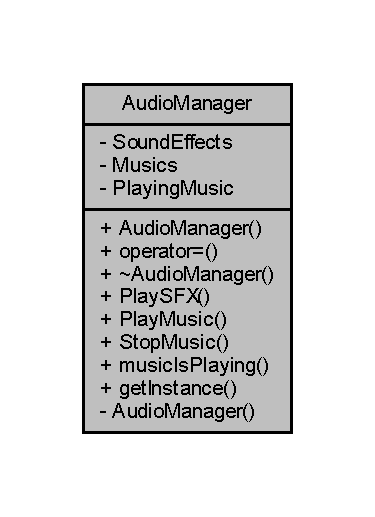
\includegraphics[width=161pt]{class_audio_manager__coll__graph}
\end{center}
\end{figure}
\subsection*{Public Member Functions}
\begin{DoxyCompactItemize}
\item 
\hyperlink{class_audio_manager_a2d67274eaba6212be9de8761439ad3ed}{\-\_\-\-\_\-declspec} (dllexport) static \hyperlink{class_audio_manager}{Audio\-Manager} \&get\-Instance()
\begin{DoxyCompactList}\small\item\em This static function returns a Singleton reference to the Audiomanager. \end{DoxyCompactList}\item 
\hyperlink{class_audio_manager_a0a4e089fd44ae9e5179fe9e0b4ea70c5}{\-\_\-\-\_\-declspec} (dllexport) \hyperlink{class_audio_manager}{Audio\-Manager}(const \hyperlink{class_audio_manager}{Audio\-Manager} \&audiomanager)=delete
\begin{DoxyCompactList}\small\item\em Deleted copy constructor. \end{DoxyCompactList}\item 
\hyperlink{class_audio_manager_a42776044d4549a30cc408be55678c8d2}{\-\_\-\-\_\-declspec} (dllexport) \hyperlink{class_audio_manager}{Audio\-Manager} \&operator
\begin{DoxyCompactList}\small\item\em Deleted assignment opperator. \end{DoxyCompactList}\item 
\hyperlink{class_audio_manager_a4e8c79c3166b6ce297cebeacf0323241}{\-\_\-\-\_\-declspec} (dllexport)$\sim$\hyperlink{class_audio_manager}{Audio\-Manager}()
\begin{DoxyCompactList}\small\item\em The Destructor. \end{DoxyCompactList}\item 
\hyperlink{class_audio_manager_ae2a3f4f84432e899de52a644c5950435}{\-\_\-\-\_\-declspec} (dllexport) bool music\-Is\-Playing()
\begin{DoxyCompactList}\small\item\em This function checks if any music is playing at the moment. \end{DoxyCompactList}\end{DoxyCompactItemize}
\subsection*{Private Member Functions}
\begin{DoxyCompactItemize}
\item 
\hyperlink{class_audio_manager_a08b3ec802ca9bdd8eda7d50e339b32ec}{\-\_\-\-\_\-declspec} (dllexport) \hyperlink{class_audio_manager}{Audio\-Manager}()
\begin{DoxyCompactList}\small\item\em The default constructor. \end{DoxyCompactList}\end{DoxyCompactItemize}
\subsection*{Private Attributes}
\begin{DoxyCompactItemize}
\item 
std\-::map$<$ std\-::string, \hyperlink{class_s_f_x}{S\-F\-X} $\ast$ $>$ \hyperlink{class_audio_manager_a3dcd808b32f86411be40485188f6a917}{Sound\-Effects}
\begin{DoxyCompactList}\small\item\em contains a key value map of strings and sound effects. \end{DoxyCompactList}\item 
std\-::map$<$ std\-::string, \\*
sf\-::\-Music $\ast$ $>$ \hyperlink{class_audio_manager_af4fd3dd64a38f93f808955a626982cc2}{Musics}
\begin{DoxyCompactList}\small\item\em contains a key value map of strings and music. \end{DoxyCompactList}\item 
sf\-::\-Music $\ast$ \hyperlink{class_audio_manager_a8309e75d7e8ac5ecf53d5d8e787d8dc8}{Playing\-Music}
\begin{DoxyCompactList}\small\item\em contains the music currently playing. \end{DoxyCompactList}\end{DoxyCompactItemize}


\subsection{Detailed Description}
This Singleton Manages and plays all music and soundeffects. 

This Class is Singleton defined. It holds an reference to all soundeffects and music. It makes sure only one song is played at a time. sound effects however can be played multiple at a time. \begin{DoxyAuthor}{Author}
Tom Verloop 
\end{DoxyAuthor}
\begin{DoxyVersion}{Version}
1.\-0 
\end{DoxyVersion}
\begin{DoxyDate}{Date}
2014-\/2015 
\end{DoxyDate}
\begin{DoxyWarning}{Warning}
A Singleton 
\end{DoxyWarning}


\subsection{Member Function Documentation}
\hypertarget{class_audio_manager_a2d67274eaba6212be9de8761439ad3ed}{\index{Audio\-Manager@{Audio\-Manager}!\-\_\-\-\_\-declspec@{\-\_\-\-\_\-declspec}}
\index{\-\_\-\-\_\-declspec@{\-\_\-\-\_\-declspec}!AudioManager@{Audio\-Manager}}
\subsubsection[{\-\_\-\-\_\-declspec}]{\setlength{\rightskip}{0pt plus 5cm}Audio\-Manager\-::\-\_\-\-\_\-declspec (
\begin{DoxyParamCaption}
\item[{dllexport}]{}
\end{DoxyParamCaption}
)}}\label{class_audio_manager_a2d67274eaba6212be9de8761439ad3ed}


This static function returns a Singleton reference to the Audiomanager. 

This function plays a uninteruptable sound effect.

\begin{DoxyReturn}{Returns}
A Refrence to the Audiomanager.
\end{DoxyReturn}

\begin{DoxyParams}[1]{Parameters}
\mbox{\tt in}  & {\em name} & contains the name of the sound effect. \\
\hline
\end{DoxyParams}
\begin{DoxyReturn}{Returns}
returns a true if the sound is available and false if not.
\end{DoxyReturn}
This function plays a interuptable music. If another was playing then it will stop that one. 
\begin{DoxyParams}[1]{Parameters}
\mbox{\tt in}  & {\em name} & contains the name of the music. \\
\hline
\end{DoxyParams}
\begin{DoxyReturn}{Returns}
returns a true if the sound is available and false if not.
\end{DoxyReturn}
This function stops any playing music except sound effects. \begin{DoxyReturn}{Returns}
returns a true if the sound is available and false if not. 
\end{DoxyReturn}
\hypertarget{class_audio_manager_a0a4e089fd44ae9e5179fe9e0b4ea70c5}{\index{Audio\-Manager@{Audio\-Manager}!\-\_\-\-\_\-declspec@{\-\_\-\-\_\-declspec}}
\index{\-\_\-\-\_\-declspec@{\-\_\-\-\_\-declspec}!AudioManager@{Audio\-Manager}}
\subsubsection[{\-\_\-\-\_\-declspec}]{\setlength{\rightskip}{0pt plus 5cm}Audio\-Manager\-::\-\_\-\-\_\-declspec (
\begin{DoxyParamCaption}
\item[{dllexport}]{}
\end{DoxyParamCaption}
) const\hspace{0.3cm}{\ttfamily [delete]}}}\label{class_audio_manager_a0a4e089fd44ae9e5179fe9e0b4ea70c5}


Deleted copy constructor. 

\hypertarget{class_audio_manager_a42776044d4549a30cc408be55678c8d2}{\index{Audio\-Manager@{Audio\-Manager}!\-\_\-\-\_\-declspec@{\-\_\-\-\_\-declspec}}
\index{\-\_\-\-\_\-declspec@{\-\_\-\-\_\-declspec}!AudioManager@{Audio\-Manager}}
\subsubsection[{\-\_\-\-\_\-declspec}]{\setlength{\rightskip}{0pt plus 5cm}Audio\-Manager\-::\-\_\-\-\_\-declspec (
\begin{DoxyParamCaption}
\item[{dllexport}]{}
\end{DoxyParamCaption}
)}}\label{class_audio_manager_a42776044d4549a30cc408be55678c8d2}


Deleted assignment opperator. 

\hypertarget{class_audio_manager_a4e8c79c3166b6ce297cebeacf0323241}{\index{Audio\-Manager@{Audio\-Manager}!\-\_\-\-\_\-declspec@{\-\_\-\-\_\-declspec}}
\index{\-\_\-\-\_\-declspec@{\-\_\-\-\_\-declspec}!AudioManager@{Audio\-Manager}}
\subsubsection[{\-\_\-\-\_\-declspec}]{\setlength{\rightskip}{0pt plus 5cm}Audio\-Manager\-::\-\_\-\-\_\-declspec (
\begin{DoxyParamCaption}
\item[{dllexport}]{}
\end{DoxyParamCaption}
)}}\label{class_audio_manager_a4e8c79c3166b6ce297cebeacf0323241}


The Destructor. 

\hypertarget{class_audio_manager_ae2a3f4f84432e899de52a644c5950435}{\index{Audio\-Manager@{Audio\-Manager}!\-\_\-\-\_\-declspec@{\-\_\-\-\_\-declspec}}
\index{\-\_\-\-\_\-declspec@{\-\_\-\-\_\-declspec}!AudioManager@{Audio\-Manager}}
\subsubsection[{\-\_\-\-\_\-declspec}]{\setlength{\rightskip}{0pt plus 5cm}Audio\-Manager\-::\-\_\-\-\_\-declspec (
\begin{DoxyParamCaption}
\item[{dllexport}]{}
\end{DoxyParamCaption}
)\hspace{0.3cm}{\ttfamily [inline]}}}\label{class_audio_manager_ae2a3f4f84432e899de52a644c5950435}


This function checks if any music is playing at the moment. 

\begin{DoxyReturn}{Returns}
returns a true if the sound is available and false if not. 
\end{DoxyReturn}
\hypertarget{class_audio_manager_a08b3ec802ca9bdd8eda7d50e339b32ec}{\index{Audio\-Manager@{Audio\-Manager}!\-\_\-\-\_\-declspec@{\-\_\-\-\_\-declspec}}
\index{\-\_\-\-\_\-declspec@{\-\_\-\-\_\-declspec}!AudioManager@{Audio\-Manager}}
\subsubsection[{\-\_\-\-\_\-declspec}]{\setlength{\rightskip}{0pt plus 5cm}Audio\-Manager\-::\-\_\-\-\_\-declspec (
\begin{DoxyParamCaption}
\item[{dllexport}]{}
\end{DoxyParamCaption}
)\hspace{0.3cm}{\ttfamily [private]}}}\label{class_audio_manager_a08b3ec802ca9bdd8eda7d50e339b32ec}


The default constructor. 



\subsection{Member Data Documentation}
\hypertarget{class_audio_manager_af4fd3dd64a38f93f808955a626982cc2}{\index{Audio\-Manager@{Audio\-Manager}!Musics@{Musics}}
\index{Musics@{Musics}!AudioManager@{Audio\-Manager}}
\subsubsection[{Musics}]{\setlength{\rightskip}{0pt plus 5cm}std\-::map$<$std\-::string, sf\-::\-Music$\ast$$>$ Audio\-Manager\-::\-Musics\hspace{0.3cm}{\ttfamily [private]}}}\label{class_audio_manager_af4fd3dd64a38f93f808955a626982cc2}


contains a key value map of strings and music. 

\hypertarget{class_audio_manager_a8309e75d7e8ac5ecf53d5d8e787d8dc8}{\index{Audio\-Manager@{Audio\-Manager}!Playing\-Music@{Playing\-Music}}
\index{Playing\-Music@{Playing\-Music}!AudioManager@{Audio\-Manager}}
\subsubsection[{Playing\-Music}]{\setlength{\rightskip}{0pt plus 5cm}sf\-::\-Music$\ast$ Audio\-Manager\-::\-Playing\-Music\hspace{0.3cm}{\ttfamily [private]}}}\label{class_audio_manager_a8309e75d7e8ac5ecf53d5d8e787d8dc8}


contains the music currently playing. 

\hypertarget{class_audio_manager_a3dcd808b32f86411be40485188f6a917}{\index{Audio\-Manager@{Audio\-Manager}!Sound\-Effects@{Sound\-Effects}}
\index{Sound\-Effects@{Sound\-Effects}!AudioManager@{Audio\-Manager}}
\subsubsection[{Sound\-Effects}]{\setlength{\rightskip}{0pt plus 5cm}std\-::map$<$std\-::string, {\bf S\-F\-X}$\ast$$>$ Audio\-Manager\-::\-Sound\-Effects\hspace{0.3cm}{\ttfamily [private]}}}\label{class_audio_manager_a3dcd808b32f86411be40485188f6a917}


contains a key value map of strings and sound effects. 



The documentation for this class was generated from the following file\-:\begin{DoxyCompactItemize}
\item 
D\-:/\-Users/tom/\-Documents/\-Visual Studio 2013/\-Projects/\-Revelatorframework/\-Revelator\-Framework\-\_\-\-A\-P\-I/\hyperlink{_audio_manager_8hpp}{Audio\-Manager.\-hpp}\end{DoxyCompactItemize}

\hypertarget{class_chunk}{\section{Chunk Class Reference}
\label{class_chunk}\index{Chunk@{Chunk}}
}


This Class represents a small portion of a screen.  




{\ttfamily \#include $<$Chunk.\-hpp$>$}



Inheritance diagram for Chunk\-:
\nopagebreak
\begin{figure}[H]
\begin{center}
\leavevmode
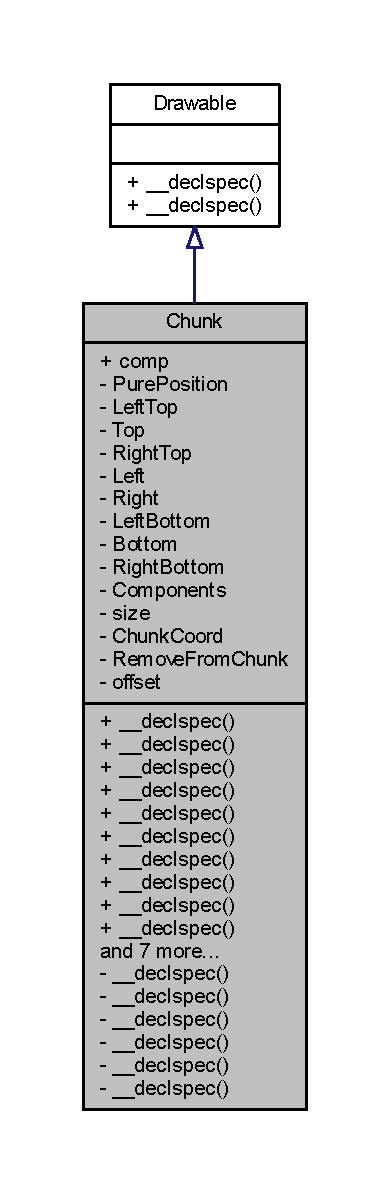
\includegraphics[height=550pt]{class_chunk__inherit__graph}
\end{center}
\end{figure}


Collaboration diagram for Chunk\-:
\nopagebreak
\begin{figure}[H]
\begin{center}
\leavevmode
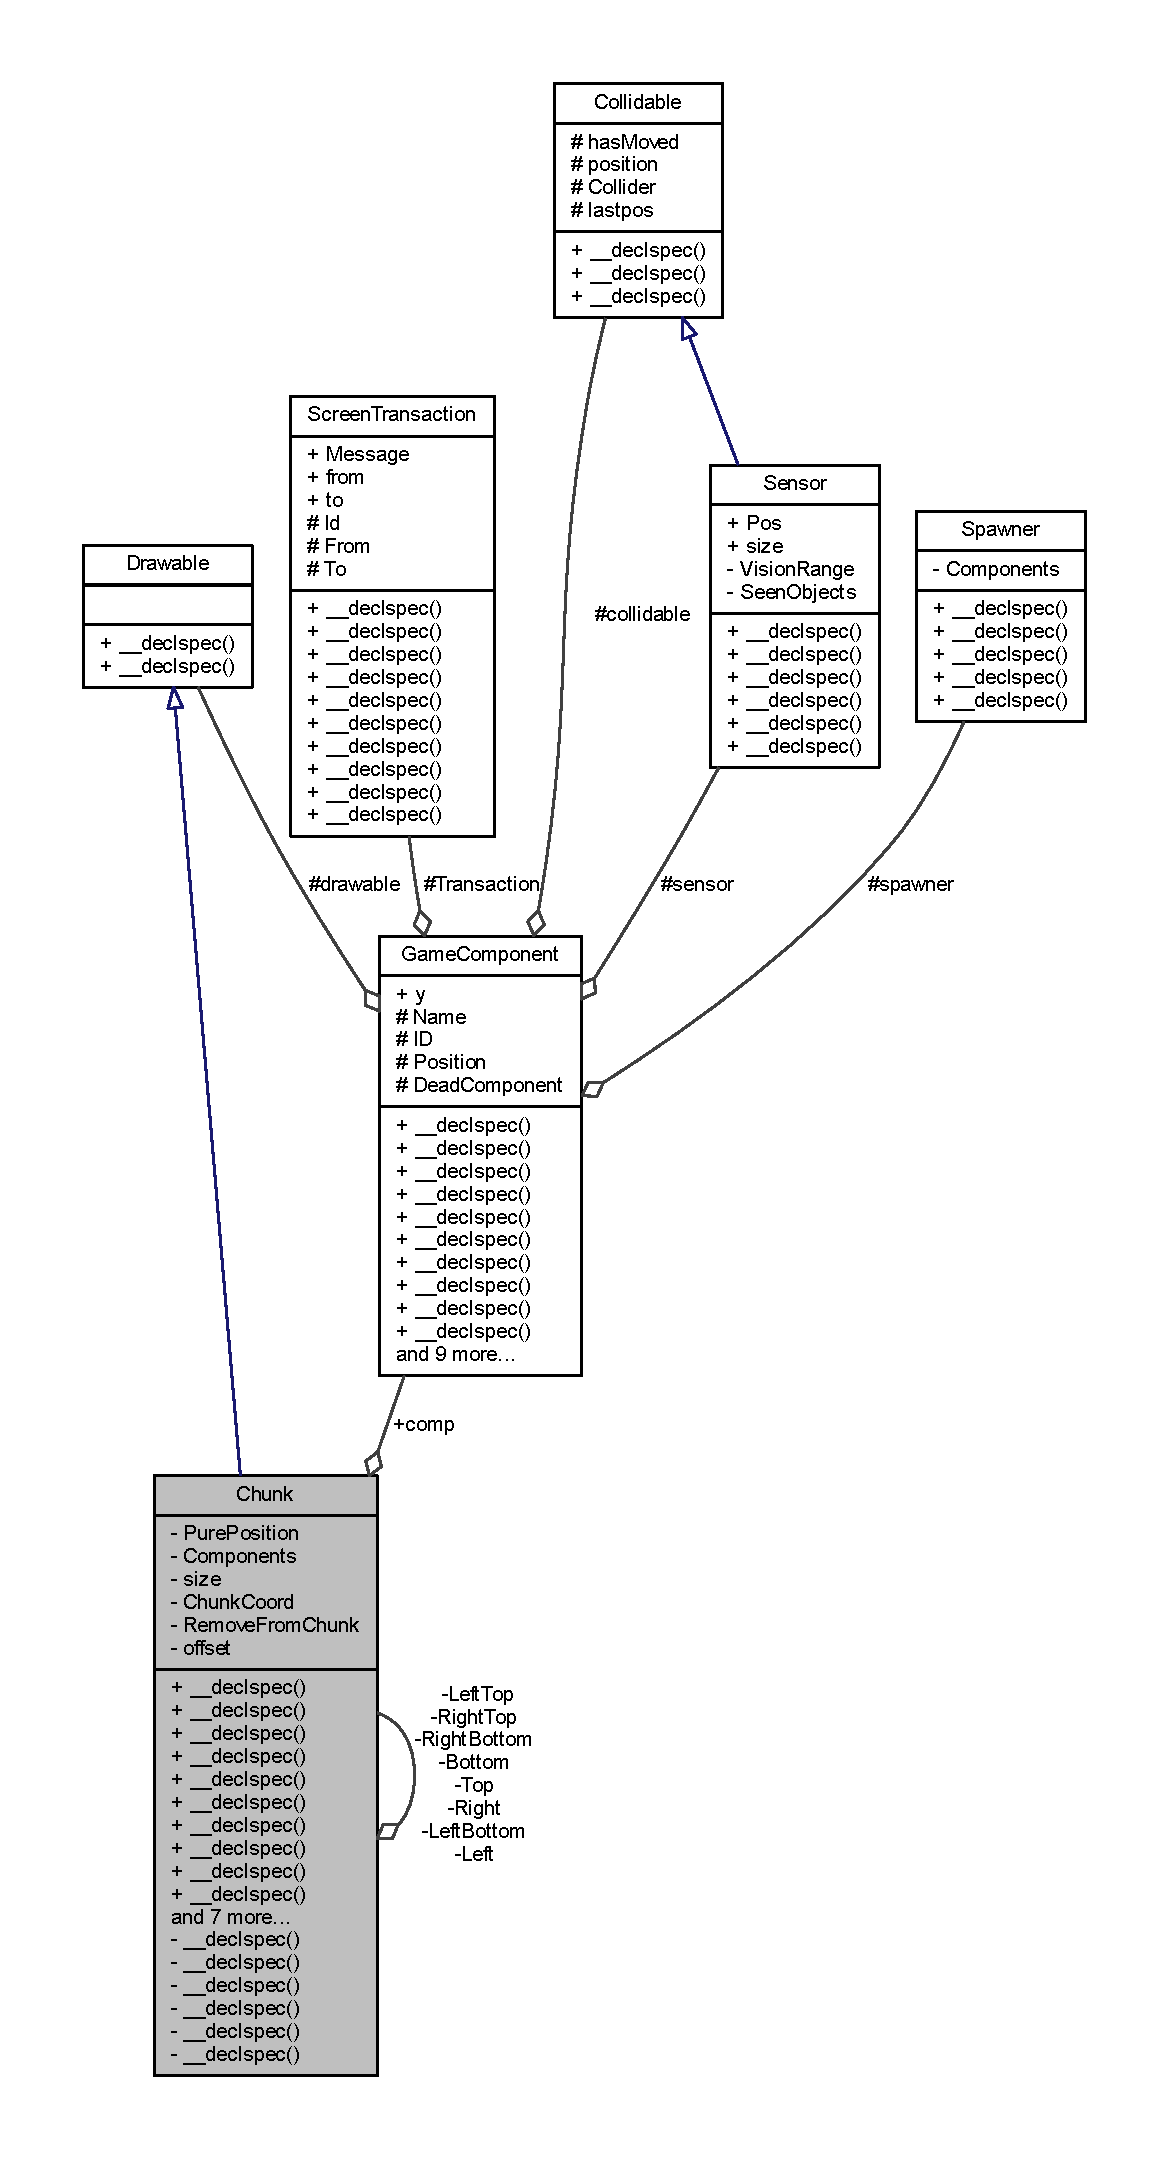
\includegraphics[height=550pt]{class_chunk__coll__graph}
\end{center}
\end{figure}
\subsection*{Public Member Functions}
\begin{DoxyCompactItemize}
\item 
\-\_\-\-\_\-declspec(dllexport) \hyperlink{class_chunk}{Chunk}(sf \hyperlink{class_chunk_ab44ec5e17f0ca6096892265ebf4a448d}{\-\_\-\-\_\-declspec} (dllexport)$\sim$\hyperlink{class_chunk}{Chunk}()
\begin{DoxyCompactList}\small\item\em The constructor. \end{DoxyCompactList}\item 
\hyperlink{class_chunk_ac74827ffc5c989b29d5ee985e0df4e96}{\-\_\-\-\_\-declspec} (dllexport) void add\-Component(\hyperlink{class_game_component}{Game\-Component} $\ast$component)
\begin{DoxyCompactList}\small\item\em This method adds a gamecomponent to the chunk or pushes it to the next if it is out of bounds. \end{DoxyCompactList}\item 
\hyperlink{class_chunk_acb635e1e8318e7b3a0accd4bcf49866d}{\-\_\-\-\_\-declspec} (dllexport) void Update(const \hyperlink{class_update_data}{Update\-Data} \&updateobject)
\begin{DoxyCompactList}\small\item\em This method pushes the update signal to all its components. \end{DoxyCompactList}\item 
\hyperlink{class_chunk_a27a4e5721687f011d6c52624d01eca8d}{\-\_\-\-\_\-declspec} (dllexport) void set\-Top(\hyperlink{class_chunk}{Chunk} $\ast$top)
\begin{DoxyCompactList}\small\item\em This method sets a chunk as the chunk to the top. \end{DoxyCompactList}\item 
\hyperlink{class_chunk_a164b8ab3a4d2e88b6d1bc5e6edfef100}{\-\_\-\-\_\-declspec} (dllexport) void set\-Right\-Top(\hyperlink{class_chunk}{Chunk} $\ast$righttop)
\begin{DoxyCompactList}\small\item\em This method sets a chunk as the chunk to the top right. \end{DoxyCompactList}\item 
\hyperlink{class_chunk_a5e25de330ba7c7c2e557a823d7a8505b}{\-\_\-\-\_\-declspec} (dllexport) void set\-Left(\hyperlink{class_chunk}{Chunk} $\ast$left)
\begin{DoxyCompactList}\small\item\em This method sets a chunk as the chunk to the left. \end{DoxyCompactList}\item 
\hyperlink{class_chunk_ac390d85879176e6e8a26667ba97f8eee}{\-\_\-\-\_\-declspec} (dllexport) void set\-Right(\hyperlink{class_chunk}{Chunk} $\ast$right)
\begin{DoxyCompactList}\small\item\em This method sets a chunk as the chunk to the right. \end{DoxyCompactList}\item 
\hyperlink{class_chunk_a5f6e70225dcd2d5f2cf0c3f77abdfa4b}{\-\_\-\-\_\-declspec} (dllexport) void set\-Left\-Bottom(\hyperlink{class_chunk}{Chunk} $\ast$leftbottom)
\begin{DoxyCompactList}\small\item\em This method sets a chunk as the chunk to the bottom left. \end{DoxyCompactList}\item 
\hyperlink{class_chunk_a69ed23533460c9308dc6ae6e92143e65}{\-\_\-\-\_\-declspec} (dllexport) void set\-Bottom(\hyperlink{class_chunk}{Chunk} $\ast$bottom)
\begin{DoxyCompactList}\small\item\em This method sets a chunk as the chunk to the bottom. \end{DoxyCompactList}\item 
\hyperlink{class_chunk_a42b5a5cf3a22b7cdd14e5e16f9c74ed0}{\-\_\-\-\_\-declspec} (dllexport) void set\-Right\-Bottom(\hyperlink{class_chunk}{Chunk} $\ast$rightbottom)
\begin{DoxyCompactList}\small\item\em This method sets a chunk as the chunk to the bottom right. \end{DoxyCompactList}\item 
\hyperlink{class_chunk_a023a2a543fc48c2b9ba5d2e31eb42e2a}{\-\_\-\-\_\-declspec} (dllexport) \hyperlink{class_chunk}{Chunk} $\ast$get\-Top()
\begin{DoxyCompactList}\small\item\em This method returns the chunk to the top. \end{DoxyCompactList}\item 
\hyperlink{class_chunk_a9b1f0c64473950040eff7ac832ae07f7}{\-\_\-\-\_\-declspec} (dllexport) \hyperlink{class_chunk}{Chunk} $\ast$get\-Left()
\begin{DoxyCompactList}\small\item\em This method returns the chunk to the left. \end{DoxyCompactList}\item 
\hyperlink{class_chunk_a55bd34d914023066cf0bdd1297c3ae8f}{\-\_\-\-\_\-declspec} (dllexport) \hyperlink{class_chunk}{Chunk} $\ast$get\-Right()
\begin{DoxyCompactList}\small\item\em This method returns the chunk to the right. \end{DoxyCompactList}\item 
\hyperlink{class_chunk_a4a65f82eed937ca57e26fbfc8b449fd2}{\-\_\-\-\_\-declspec} (dllexport) \hyperlink{class_chunk}{Chunk} $\ast$get\-Bottom()
\begin{DoxyCompactList}\small\item\em This method returns the chunk to the bottom. \end{DoxyCompactList}\item 
\hyperlink{class_chunk_a11a6eb32b5444ba24bb506e1a57ad4b8}{\-\_\-\-\_\-declspec} (dllexport) sf
\begin{DoxyCompactList}\small\item\em This method returns the chunk coordinates. \end{DoxyCompactList}\item 
\hyperlink{class_chunk_a2a4b74bc2a675752c97407233d14cbaf}{\-\_\-\-\_\-declspec} (dllexport) void Sense\-Single(const \hyperlink{class_update_data}{Update\-Data} \&updateobject
\begin{DoxyCompactList}\small\item\em This method calculates the vision of a single component. \end{DoxyCompactList}\item 
\hyperlink{class_chunk_aabce986183d5f99c1c89a80b51127aa9}{\-\_\-\-\_\-declspec} (dllexport) void Collide\-Single(const \hyperlink{class_update_data}{Update\-Data} \&updateobject
\begin{DoxyCompactList}\small\item\em This method calculates the collision of a single component. \end{DoxyCompactList}\item 
\hyperlink{class_chunk_a11a6eb32b5444ba24bb506e1a57ad4b8}{\-\_\-\-\_\-declspec} (dllexport) sf
\begin{DoxyCompactList}\small\item\em This method returns the real position of the chunk. \end{DoxyCompactList}\item 
\hyperlink{class_chunk_acf3fa4e0c9a7ef9c820c3ba001e449fb}{\-\_\-\-\_\-declspec} (dllexport) float get\-Size()
\begin{DoxyCompactList}\small\item\em This method returns the size of the chunk. \end{DoxyCompactList}\end{DoxyCompactItemize}
\subsection*{Public Attributes}
\begin{DoxyCompactItemize}
\item 
\hyperlink{class_game_component}{Game\-Component} $\ast$ \hyperlink{class_chunk_a633545d862acb016a7081c364126c7b8}{comp}
\end{DoxyCompactItemize}
\subsection*{Private Member Functions}
\begin{DoxyCompactItemize}
\item 
\hyperlink{class_chunk_a09fed540af40e1ad76e8ef2babbfe616}{\-\_\-\-\_\-declspec} (dllexport) void Collide(const \hyperlink{class_update_data}{Update\-Data} \&updateobject)
\begin{DoxyCompactList}\small\item\em This method calls Chunk\-::\-Collide\-Single for every component in the chunk. \end{DoxyCompactList}\item 
\hyperlink{class_chunk_a8a24db04cbc32e330b07d34caa61eeb1}{\-\_\-\-\_\-declspec} (dllexport) void Sense(const \hyperlink{class_update_data}{Update\-Data} \&updateobject)
\begin{DoxyCompactList}\small\item\em This method calls Chunk\-::\-Sense\-Single for every component in the chunk. \end{DoxyCompactList}\item 
\hyperlink{class_chunk_a5c65ce716caab3e2c5bd9193f8e29888}{\-\_\-\-\_\-declspec} (dllexport) void Move\-Component\-To\-Next\-Chunk(\hyperlink{class_game_component}{Game\-Component} $\ast$c)
\begin{DoxyCompactList}\small\item\em This method checks if a component still resides inside the chunk if not it will push it to the next chunk. if no next chunk exsists it will pull the component back into its region. \end{DoxyCompactList}\item 
\hyperlink{class_chunk_aad4ce00be30a71cddc9a17226a992a0f}{\-\_\-\-\_\-declspec} (dllexport) bool Axisis\-In\-Bounds(float axis
\begin{DoxyCompactList}\small\item\em a function to simplify the ifstatements in Chunk\-::\-Move\-Component\-To\-Next\-Chunk \end{DoxyCompactList}\item 
\hyperlink{class_chunk_aecb19003f0e0330920cf7695fbdc5700}{\-\_\-\-\_\-declspec} (dllexport) void Remove\-Flagged\-From\-Chunk()
\begin{DoxyCompactList}\small\item\em removes all the \char`\"{}\-Dead\char`\"{} components from the chunk but does not delete them. \end{DoxyCompactList}\end{DoxyCompactItemize}
\subsection*{Private Attributes}
\begin{DoxyCompactItemize}
\item 
sf\-::\-Vector2f \hyperlink{class_chunk_ace1577872b1189bc7fd88a9b3817ce98}{Pure\-Position}
\begin{DoxyCompactList}\small\item\em Contains the real position of the chunk. \end{DoxyCompactList}\item 
\hyperlink{class_chunk}{Chunk} $\ast$ \hyperlink{class_chunk_a877d51226eaa97c40c05223987514d59}{Left\-Top}
\begin{DoxyCompactList}\small\item\em contains a pointer to the topleft chunk. \end{DoxyCompactList}\item 
\hyperlink{class_chunk}{Chunk} $\ast$ \hyperlink{class_chunk_ae841d5ab24dfa5ef8865cb4fa05d089d}{Top}
\begin{DoxyCompactList}\small\item\em contains a pointer to the top chunk. \end{DoxyCompactList}\item 
\hyperlink{class_chunk}{Chunk} $\ast$ \hyperlink{class_chunk_a8a7593c89d4fe5ed193e68b9ed40016b}{Right\-Top}
\begin{DoxyCompactList}\small\item\em contains a pointer to the topright chunk. \end{DoxyCompactList}\item 
\hyperlink{class_chunk}{Chunk} $\ast$ \hyperlink{class_chunk_aee27c2584364a58dc8811e9ada0695dd}{Left}
\begin{DoxyCompactList}\small\item\em contains a pointer to the left chunk. \end{DoxyCompactList}\item 
\hyperlink{class_chunk}{Chunk} $\ast$ \hyperlink{class_chunk_a0bcf134e2aba0ca49370272c2b3f17a4}{Right}
\begin{DoxyCompactList}\small\item\em contains a pointer to the right chunk. \end{DoxyCompactList}\item 
\hyperlink{class_chunk}{Chunk} $\ast$ \hyperlink{class_chunk_af3577f37139ffeb74181d9ce3c48f5e6}{Left\-Bottom}
\begin{DoxyCompactList}\small\item\em contains a pointer to the bottomleft chunk. \end{DoxyCompactList}\item 
\hyperlink{class_chunk}{Chunk} $\ast$ \hyperlink{class_chunk_ac9ac53a727ae045b6f751ec6a68bcaca}{Bottom}
\begin{DoxyCompactList}\small\item\em contains a pointer to the bottom chunk. \end{DoxyCompactList}\item 
\hyperlink{class_chunk}{Chunk} $\ast$ \hyperlink{class_chunk_afded01a9a67540c9f64dde5776021f4b}{Right\-Bottom}
\begin{DoxyCompactList}\small\item\em contains a pointer to the bottomright chunk. \end{DoxyCompactList}\item 
std\-::list$<$ \hyperlink{class_game_component}{Game\-Component} $\ast$ $>$ \hyperlink{class_chunk_a4cdf6febd96ff99b681e37d548617a38}{Components}
\begin{DoxyCompactList}\small\item\em contains a list of components contained in the chunk. \end{DoxyCompactList}\item 
float \hyperlink{class_chunk_af46410b580baf2985b01044d5c041b2e}{size}
\begin{DoxyCompactList}\small\item\em contains the size of the chunk. \end{DoxyCompactList}\item 
sf\-::\-Vector2i \hyperlink{class_chunk_abb5b1842148b3d7c616065766bfd2b33}{Chunk\-Coord}
\begin{DoxyCompactList}\small\item\em contains the coordinates of the chunk \end{DoxyCompactList}\item 
std\-::list$<$ \hyperlink{class_game_component}{Game\-Component} $\ast$ $>$ \hyperlink{class_chunk_adf6692fdab4518524e217cc0ef09d282}{Remove\-From\-Chunk}
\begin{DoxyCompactList}\small\item\em contains a list of components to remove from the chunk. \end{DoxyCompactList}\item 
float \hyperlink{class_chunk_a6ab7f8f3970c886a62ccc1630bc60a16}{offset}
\end{DoxyCompactItemize}


\subsection{Detailed Description}
This Class represents a small portion of a screen. 

This Class represents a small portion of a screen. it makes sure nothing more is drawn than necessary. It handles its own draw and that of the neigboring chunks. and it holds all components that are at its location. further more it handles the vision and collision of the components in it. \begin{DoxyAuthor}{Author}
Tom Verloop 
\end{DoxyAuthor}
\begin{DoxyVersion}{Version}
1.\-0 
\end{DoxyVersion}
\begin{DoxyDate}{Date}
2014-\/2015 
\end{DoxyDate}
\begin{DoxyRefDesc}{Bug}
\item[\hyperlink{bug__bug000001}{Bug}]anything with a vision greater that one chunk next to it is useless. \end{DoxyRefDesc}


\subsection{Member Function Documentation}
\hypertarget{class_chunk_ab44ec5e17f0ca6096892265ebf4a448d}{\index{Chunk@{Chunk}!\-\_\-\-\_\-declspec@{\-\_\-\-\_\-declspec}}
\index{\-\_\-\-\_\-declspec@{\-\_\-\-\_\-declspec}!Chunk@{Chunk}}
\subsubsection[{\-\_\-\-\_\-declspec}]{\setlength{\rightskip}{0pt plus 5cm}Chunk\-::\-\_\-\-\_\-declspec (
\begin{DoxyParamCaption}
\item[{dllexport}]{}
\end{DoxyParamCaption}
)}}\label{class_chunk_ab44ec5e17f0ca6096892265ebf4a448d}


The constructor. 

This method pushes the Draw\-Self signal to all its neighboring chunks and itself.


\begin{DoxyParams}[1]{Parameters}
\mbox{\tt in}  & {\em Chunk\-Coord} & contains the coordinates used to calculate its real position on the screen. \\
\hline
\mbox{\tt in}  & {\em size} & contains the size of the chunk used to contain its components in.\\
\hline
\end{DoxyParams}
The Deconstructor.


\begin{DoxyParams}[1]{Parameters}
\mbox{\tt in}  & {\em window} & holds an reference to the renderwindow to draw upon. \\
\hline
\mbox{\tt in}  & {\em offset} & holds an position to add to the one of the component.\\
\hline
\end{DoxyParams}
This method pushes the draw signal to all its components. 
\begin{DoxyParams}[1]{Parameters}
\mbox{\tt in}  & {\em window} & holds an reference to the renderwindow to draw upon. \\
\hline
\mbox{\tt in}  & {\em offset} & holds an position to add to the one of the component. \\
\hline
\mbox{\tt in}  & {\em offset} & holds an position from where the draw method was called on the screen.\\
\hline
\end{DoxyParams}
This method sets a chunk as the chunk to the top left. 
\begin{DoxyParams}[1]{Parameters}
\mbox{\tt in}  & {\em lefttop} & contains a pointer to the chunk that should be to the top left. \\
\hline
\end{DoxyParams}
\hypertarget{class_chunk_ac74827ffc5c989b29d5ee985e0df4e96}{\index{Chunk@{Chunk}!\-\_\-\-\_\-declspec@{\-\_\-\-\_\-declspec}}
\index{\-\_\-\-\_\-declspec@{\-\_\-\-\_\-declspec}!Chunk@{Chunk}}
\subsubsection[{\-\_\-\-\_\-declspec}]{\setlength{\rightskip}{0pt plus 5cm}Chunk\-::\-\_\-\-\_\-declspec (
\begin{DoxyParamCaption}
\item[{dllexport}]{}
\end{DoxyParamCaption}
)}}\label{class_chunk_ac74827ffc5c989b29d5ee985e0df4e96}


This method adds a gamecomponent to the chunk or pushes it to the next if it is out of bounds. 


\begin{DoxyParams}[1]{Parameters}
\mbox{\tt in}  & {\em component} & contains a pointer to the component it is supposed to hold. \\
\hline
\end{DoxyParams}
\hypertarget{class_chunk_acb635e1e8318e7b3a0accd4bcf49866d}{\index{Chunk@{Chunk}!\-\_\-\-\_\-declspec@{\-\_\-\-\_\-declspec}}
\index{\-\_\-\-\_\-declspec@{\-\_\-\-\_\-declspec}!Chunk@{Chunk}}
\subsubsection[{\-\_\-\-\_\-declspec}]{\setlength{\rightskip}{0pt plus 5cm}Chunk\-::\-\_\-\-\_\-declspec (
\begin{DoxyParamCaption}
\item[{dllexport}]{}
\end{DoxyParamCaption}
) const}}\label{class_chunk_acb635e1e8318e7b3a0accd4bcf49866d}


This method pushes the update signal to all its components. 


\begin{DoxyParams}[1]{Parameters}
\mbox{\tt in}  & {\em updateobject} & contains a reference to the updateobject containing updatedata. \\
\hline
\end{DoxyParams}
\hypertarget{class_chunk_a27a4e5721687f011d6c52624d01eca8d}{\index{Chunk@{Chunk}!\-\_\-\-\_\-declspec@{\-\_\-\-\_\-declspec}}
\index{\-\_\-\-\_\-declspec@{\-\_\-\-\_\-declspec}!Chunk@{Chunk}}
\subsubsection[{\-\_\-\-\_\-declspec}]{\setlength{\rightskip}{0pt plus 5cm}Chunk\-::\-\_\-\-\_\-declspec (
\begin{DoxyParamCaption}
\item[{dllexport}]{}
\end{DoxyParamCaption}
)}}\label{class_chunk_a27a4e5721687f011d6c52624d01eca8d}


This method sets a chunk as the chunk to the top. 


\begin{DoxyParams}[1]{Parameters}
\mbox{\tt in}  & {\em top} & contains a pointer to the chunk that should be to the top. \\
\hline
\end{DoxyParams}
\hypertarget{class_chunk_a164b8ab3a4d2e88b6d1bc5e6edfef100}{\index{Chunk@{Chunk}!\-\_\-\-\_\-declspec@{\-\_\-\-\_\-declspec}}
\index{\-\_\-\-\_\-declspec@{\-\_\-\-\_\-declspec}!Chunk@{Chunk}}
\subsubsection[{\-\_\-\-\_\-declspec}]{\setlength{\rightskip}{0pt plus 5cm}Chunk\-::\-\_\-\-\_\-declspec (
\begin{DoxyParamCaption}
\item[{dllexport}]{}
\end{DoxyParamCaption}
)}}\label{class_chunk_a164b8ab3a4d2e88b6d1bc5e6edfef100}


This method sets a chunk as the chunk to the top right. 


\begin{DoxyParams}[1]{Parameters}
\mbox{\tt in}  & {\em righttop} & contains a pointer to the chunk that should be to the top right. \\
\hline
\end{DoxyParams}
\hypertarget{class_chunk_a5e25de330ba7c7c2e557a823d7a8505b}{\index{Chunk@{Chunk}!\-\_\-\-\_\-declspec@{\-\_\-\-\_\-declspec}}
\index{\-\_\-\-\_\-declspec@{\-\_\-\-\_\-declspec}!Chunk@{Chunk}}
\subsubsection[{\-\_\-\-\_\-declspec}]{\setlength{\rightskip}{0pt plus 5cm}Chunk\-::\-\_\-\-\_\-declspec (
\begin{DoxyParamCaption}
\item[{dllexport}]{}
\end{DoxyParamCaption}
)}}\label{class_chunk_a5e25de330ba7c7c2e557a823d7a8505b}


This method sets a chunk as the chunk to the left. 


\begin{DoxyParams}[1]{Parameters}
\mbox{\tt in}  & {\em left} & contains a pointer to the chunk that should be to the left. \\
\hline
\end{DoxyParams}
\hypertarget{class_chunk_ac390d85879176e6e8a26667ba97f8eee}{\index{Chunk@{Chunk}!\-\_\-\-\_\-declspec@{\-\_\-\-\_\-declspec}}
\index{\-\_\-\-\_\-declspec@{\-\_\-\-\_\-declspec}!Chunk@{Chunk}}
\subsubsection[{\-\_\-\-\_\-declspec}]{\setlength{\rightskip}{0pt plus 5cm}Chunk\-::\-\_\-\-\_\-declspec (
\begin{DoxyParamCaption}
\item[{dllexport}]{}
\end{DoxyParamCaption}
)}}\label{class_chunk_ac390d85879176e6e8a26667ba97f8eee}


This method sets a chunk as the chunk to the right. 


\begin{DoxyParams}[1]{Parameters}
\mbox{\tt in}  & {\em right} & contains a pointer to the chunk that should be to the right. \\
\hline
\end{DoxyParams}
\hypertarget{class_chunk_a5f6e70225dcd2d5f2cf0c3f77abdfa4b}{\index{Chunk@{Chunk}!\-\_\-\-\_\-declspec@{\-\_\-\-\_\-declspec}}
\index{\-\_\-\-\_\-declspec@{\-\_\-\-\_\-declspec}!Chunk@{Chunk}}
\subsubsection[{\-\_\-\-\_\-declspec}]{\setlength{\rightskip}{0pt plus 5cm}Chunk\-::\-\_\-\-\_\-declspec (
\begin{DoxyParamCaption}
\item[{dllexport}]{}
\end{DoxyParamCaption}
)}}\label{class_chunk_a5f6e70225dcd2d5f2cf0c3f77abdfa4b}


This method sets a chunk as the chunk to the bottom left. 


\begin{DoxyParams}[1]{Parameters}
\mbox{\tt in}  & {\em leftbottom} & contains a pointer to the chunk that should be to the bottom left. \\
\hline
\end{DoxyParams}
\hypertarget{class_chunk_a69ed23533460c9308dc6ae6e92143e65}{\index{Chunk@{Chunk}!\-\_\-\-\_\-declspec@{\-\_\-\-\_\-declspec}}
\index{\-\_\-\-\_\-declspec@{\-\_\-\-\_\-declspec}!Chunk@{Chunk}}
\subsubsection[{\-\_\-\-\_\-declspec}]{\setlength{\rightskip}{0pt plus 5cm}Chunk\-::\-\_\-\-\_\-declspec (
\begin{DoxyParamCaption}
\item[{dllexport}]{}
\end{DoxyParamCaption}
)}}\label{class_chunk_a69ed23533460c9308dc6ae6e92143e65}


This method sets a chunk as the chunk to the bottom. 


\begin{DoxyParams}[1]{Parameters}
\mbox{\tt in}  & {\em bottom} & contains a pointer to the chunk that should be to the bottom. \\
\hline
\end{DoxyParams}
\hypertarget{class_chunk_a42b5a5cf3a22b7cdd14e5e16f9c74ed0}{\index{Chunk@{Chunk}!\-\_\-\-\_\-declspec@{\-\_\-\-\_\-declspec}}
\index{\-\_\-\-\_\-declspec@{\-\_\-\-\_\-declspec}!Chunk@{Chunk}}
\subsubsection[{\-\_\-\-\_\-declspec}]{\setlength{\rightskip}{0pt plus 5cm}Chunk\-::\-\_\-\-\_\-declspec (
\begin{DoxyParamCaption}
\item[{dllexport}]{}
\end{DoxyParamCaption}
)}}\label{class_chunk_a42b5a5cf3a22b7cdd14e5e16f9c74ed0}


This method sets a chunk as the chunk to the bottom right. 


\begin{DoxyParams}[1]{Parameters}
\mbox{\tt in}  & {\em rightbottom} & contains a pointer to the chunk that should be to the bottom right. \\
\hline
\end{DoxyParams}
\hypertarget{class_chunk_a023a2a543fc48c2b9ba5d2e31eb42e2a}{\index{Chunk@{Chunk}!\-\_\-\-\_\-declspec@{\-\_\-\-\_\-declspec}}
\index{\-\_\-\-\_\-declspec@{\-\_\-\-\_\-declspec}!Chunk@{Chunk}}
\subsubsection[{\-\_\-\-\_\-declspec}]{\setlength{\rightskip}{0pt plus 5cm}Chunk\-::\-\_\-\-\_\-declspec (
\begin{DoxyParamCaption}
\item[{dllexport}]{}
\end{DoxyParamCaption}
)}}\label{class_chunk_a023a2a543fc48c2b9ba5d2e31eb42e2a}


This method returns the chunk to the top. 

\begin{DoxyReturn}{Returns}
A pointer of the chunk to the top. 
\end{DoxyReturn}
\hypertarget{class_chunk_a9b1f0c64473950040eff7ac832ae07f7}{\index{Chunk@{Chunk}!\-\_\-\-\_\-declspec@{\-\_\-\-\_\-declspec}}
\index{\-\_\-\-\_\-declspec@{\-\_\-\-\_\-declspec}!Chunk@{Chunk}}
\subsubsection[{\-\_\-\-\_\-declspec}]{\setlength{\rightskip}{0pt plus 5cm}Chunk\-::\-\_\-\-\_\-declspec (
\begin{DoxyParamCaption}
\item[{dllexport}]{}
\end{DoxyParamCaption}
)}}\label{class_chunk_a9b1f0c64473950040eff7ac832ae07f7}


This method returns the chunk to the left. 

\begin{DoxyReturn}{Returns}
A pointer of the chunk to the left. 
\end{DoxyReturn}
\hypertarget{class_chunk_a55bd34d914023066cf0bdd1297c3ae8f}{\index{Chunk@{Chunk}!\-\_\-\-\_\-declspec@{\-\_\-\-\_\-declspec}}
\index{\-\_\-\-\_\-declspec@{\-\_\-\-\_\-declspec}!Chunk@{Chunk}}
\subsubsection[{\-\_\-\-\_\-declspec}]{\setlength{\rightskip}{0pt plus 5cm}Chunk\-::\-\_\-\-\_\-declspec (
\begin{DoxyParamCaption}
\item[{dllexport}]{}
\end{DoxyParamCaption}
)}}\label{class_chunk_a55bd34d914023066cf0bdd1297c3ae8f}


This method returns the chunk to the right. 

\begin{DoxyReturn}{Returns}
A pointer of the chunk to the right. 
\end{DoxyReturn}
\hypertarget{class_chunk_a4a65f82eed937ca57e26fbfc8b449fd2}{\index{Chunk@{Chunk}!\-\_\-\-\_\-declspec@{\-\_\-\-\_\-declspec}}
\index{\-\_\-\-\_\-declspec@{\-\_\-\-\_\-declspec}!Chunk@{Chunk}}
\subsubsection[{\-\_\-\-\_\-declspec}]{\setlength{\rightskip}{0pt plus 5cm}Chunk\-::\-\_\-\-\_\-declspec (
\begin{DoxyParamCaption}
\item[{dllexport}]{}
\end{DoxyParamCaption}
)}}\label{class_chunk_a4a65f82eed937ca57e26fbfc8b449fd2}


This method returns the chunk to the bottom. 

\begin{DoxyReturn}{Returns}
A pointer of the chunk to the bottom. 
\end{DoxyReturn}
\hypertarget{class_chunk_a11a6eb32b5444ba24bb506e1a57ad4b8}{\index{Chunk@{Chunk}!\-\_\-\-\_\-declspec@{\-\_\-\-\_\-declspec}}
\index{\-\_\-\-\_\-declspec@{\-\_\-\-\_\-declspec}!Chunk@{Chunk}}
\subsubsection[{\-\_\-\-\_\-declspec}]{\setlength{\rightskip}{0pt plus 5cm}Chunk\-::\-\_\-\-\_\-declspec (
\begin{DoxyParamCaption}
\item[{dllexport}]{}
\end{DoxyParamCaption}
)\hspace{0.3cm}{\ttfamily [inline]}}}\label{class_chunk_a11a6eb32b5444ba24bb506e1a57ad4b8}


This method returns the chunk coordinates. 

\begin{DoxyReturn}{Returns}
A 2d integer vector. 
\end{DoxyReturn}
\hypertarget{class_chunk_a2a4b74bc2a675752c97407233d14cbaf}{\index{Chunk@{Chunk}!\-\_\-\-\_\-declspec@{\-\_\-\-\_\-declspec}}
\index{\-\_\-\-\_\-declspec@{\-\_\-\-\_\-declspec}!Chunk@{Chunk}}
\subsubsection[{\-\_\-\-\_\-declspec}]{\setlength{\rightskip}{0pt plus 5cm}Chunk\-::\-\_\-\-\_\-declspec (
\begin{DoxyParamCaption}
\item[{dllexport}]{}
\end{DoxyParamCaption}
) const}}\label{class_chunk_a2a4b74bc2a675752c97407233d14cbaf}


This method calculates the vision of a single component. 


\begin{DoxyParams}[1]{Parameters}
\mbox{\tt in}  & {\em updateobject} & Contains all data required for the update event. \\
\hline
\mbox{\tt out}  & {\em comp} & Contains the game component who is sensing for other components. \\
\hline
\end{DoxyParams}
\hypertarget{class_chunk_aabce986183d5f99c1c89a80b51127aa9}{\index{Chunk@{Chunk}!\-\_\-\-\_\-declspec@{\-\_\-\-\_\-declspec}}
\index{\-\_\-\-\_\-declspec@{\-\_\-\-\_\-declspec}!Chunk@{Chunk}}
\subsubsection[{\-\_\-\-\_\-declspec}]{\setlength{\rightskip}{0pt plus 5cm}Chunk\-::\-\_\-\-\_\-declspec (
\begin{DoxyParamCaption}
\item[{dllexport}]{}
\end{DoxyParamCaption}
) const}}\label{class_chunk_aabce986183d5f99c1c89a80b51127aa9}


This method calculates the collision of a single component. 


\begin{DoxyParams}[1]{Parameters}
\mbox{\tt in}  & {\em updateobject} & Contains all data required for the update event. \\
\hline
\mbox{\tt out}  & {\em comp} & Contains the game component who is colliding with other components. \\
\hline
\end{DoxyParams}
\hypertarget{class_chunk_a11a6eb32b5444ba24bb506e1a57ad4b8}{\index{Chunk@{Chunk}!\-\_\-\-\_\-declspec@{\-\_\-\-\_\-declspec}}
\index{\-\_\-\-\_\-declspec@{\-\_\-\-\_\-declspec}!Chunk@{Chunk}}
\subsubsection[{\-\_\-\-\_\-declspec}]{\setlength{\rightskip}{0pt plus 5cm}Chunk\-::\-\_\-\-\_\-declspec (
\begin{DoxyParamCaption}
\item[{dllexport}]{}
\end{DoxyParamCaption}
)\hspace{0.3cm}{\ttfamily [inline]}}}\label{class_chunk_a11a6eb32b5444ba24bb506e1a57ad4b8}


This method returns the real position of the chunk. 

\begin{DoxyReturn}{Returns}
A 2\-D float vector containing the position of the chunk. 
\end{DoxyReturn}
\hypertarget{class_chunk_acf3fa4e0c9a7ef9c820c3ba001e449fb}{\index{Chunk@{Chunk}!\-\_\-\-\_\-declspec@{\-\_\-\-\_\-declspec}}
\index{\-\_\-\-\_\-declspec@{\-\_\-\-\_\-declspec}!Chunk@{Chunk}}
\subsubsection[{\-\_\-\-\_\-declspec}]{\setlength{\rightskip}{0pt plus 5cm}Chunk\-::\-\_\-\-\_\-declspec (
\begin{DoxyParamCaption}
\item[{dllexport}]{}
\end{DoxyParamCaption}
)\hspace{0.3cm}{\ttfamily [inline]}}}\label{class_chunk_acf3fa4e0c9a7ef9c820c3ba001e449fb}


This method returns the size of the chunk. 

\begin{DoxyReturn}{Returns}
A float containing the size of the chunk. 
\end{DoxyReturn}
\hypertarget{class_chunk_a09fed540af40e1ad76e8ef2babbfe616}{\index{Chunk@{Chunk}!\-\_\-\-\_\-declspec@{\-\_\-\-\_\-declspec}}
\index{\-\_\-\-\_\-declspec@{\-\_\-\-\_\-declspec}!Chunk@{Chunk}}
\subsubsection[{\-\_\-\-\_\-declspec}]{\setlength{\rightskip}{0pt plus 5cm}Chunk\-::\-\_\-\-\_\-declspec (
\begin{DoxyParamCaption}
\item[{dllexport}]{}
\end{DoxyParamCaption}
) const\hspace{0.3cm}{\ttfamily [private]}}}\label{class_chunk_a09fed540af40e1ad76e8ef2babbfe616}


This method calls Chunk\-::\-Collide\-Single for every component in the chunk. 


\begin{DoxyParams}[1]{Parameters}
\mbox{\tt in}  & {\em updateobject} & contains all data for the update event. \\
\hline
\end{DoxyParams}
\hypertarget{class_chunk_a8a24db04cbc32e330b07d34caa61eeb1}{\index{Chunk@{Chunk}!\-\_\-\-\_\-declspec@{\-\_\-\-\_\-declspec}}
\index{\-\_\-\-\_\-declspec@{\-\_\-\-\_\-declspec}!Chunk@{Chunk}}
\subsubsection[{\-\_\-\-\_\-declspec}]{\setlength{\rightskip}{0pt plus 5cm}Chunk\-::\-\_\-\-\_\-declspec (
\begin{DoxyParamCaption}
\item[{dllexport}]{}
\end{DoxyParamCaption}
) const\hspace{0.3cm}{\ttfamily [private]}}}\label{class_chunk_a8a24db04cbc32e330b07d34caa61eeb1}


This method calls Chunk\-::\-Sense\-Single for every component in the chunk. 


\begin{DoxyParams}[1]{Parameters}
\mbox{\tt in}  & {\em updateobject} & contains all data for the update event. \\
\hline
\end{DoxyParams}
\hypertarget{class_chunk_a5c65ce716caab3e2c5bd9193f8e29888}{\index{Chunk@{Chunk}!\-\_\-\-\_\-declspec@{\-\_\-\-\_\-declspec}}
\index{\-\_\-\-\_\-declspec@{\-\_\-\-\_\-declspec}!Chunk@{Chunk}}
\subsubsection[{\-\_\-\-\_\-declspec}]{\setlength{\rightskip}{0pt plus 5cm}Chunk\-::\-\_\-\-\_\-declspec (
\begin{DoxyParamCaption}
\item[{dllexport}]{}
\end{DoxyParamCaption}
)\hspace{0.3cm}{\ttfamily [private]}}}\label{class_chunk_a5c65ce716caab3e2c5bd9193f8e29888}


This method checks if a component still resides inside the chunk if not it will push it to the next chunk. if no next chunk exsists it will pull the component back into its region. 


\begin{DoxyParams}[1]{Parameters}
\mbox{\tt in}  & {\em c} & Contains the component to check. \\
\hline
\end{DoxyParams}
\hypertarget{class_chunk_aad4ce00be30a71cddc9a17226a992a0f}{\index{Chunk@{Chunk}!\-\_\-\-\_\-declspec@{\-\_\-\-\_\-declspec}}
\index{\-\_\-\-\_\-declspec@{\-\_\-\-\_\-declspec}!Chunk@{Chunk}}
\subsubsection[{\-\_\-\-\_\-declspec}]{\setlength{\rightskip}{0pt plus 5cm}Chunk\-::\-\_\-\-\_\-declspec (
\begin{DoxyParamCaption}
\item[{dllexport}]{}
\end{DoxyParamCaption}
)\hspace{0.3cm}{\ttfamily [private]}}}\label{class_chunk_aad4ce00be30a71cddc9a17226a992a0f}


a function to simplify the ifstatements in Chunk\-::\-Move\-Component\-To\-Next\-Chunk 


\begin{DoxyParams}[1]{Parameters}
\mbox{\tt in}  & {\em axis} & Contains the axis to check on. \\
\hline
\mbox{\tt in}  & {\em offset} & Contains the offset to check on. \\
\hline
\end{DoxyParams}
\begin{DoxyReturn}{Returns}
Returns true if the axis is in bounds. 
\end{DoxyReturn}
\hypertarget{class_chunk_aecb19003f0e0330920cf7695fbdc5700}{\index{Chunk@{Chunk}!\-\_\-\-\_\-declspec@{\-\_\-\-\_\-declspec}}
\index{\-\_\-\-\_\-declspec@{\-\_\-\-\_\-declspec}!Chunk@{Chunk}}
\subsubsection[{\-\_\-\-\_\-declspec}]{\setlength{\rightskip}{0pt plus 5cm}Chunk\-::\-\_\-\-\_\-declspec (
\begin{DoxyParamCaption}
\item[{dllexport}]{}
\end{DoxyParamCaption}
)\hspace{0.3cm}{\ttfamily [private]}}}\label{class_chunk_aecb19003f0e0330920cf7695fbdc5700}


removes all the \char`\"{}\-Dead\char`\"{} components from the chunk but does not delete them. 



\subsection{Member Data Documentation}
\hypertarget{class_chunk_ac9ac53a727ae045b6f751ec6a68bcaca}{\index{Chunk@{Chunk}!Bottom@{Bottom}}
\index{Bottom@{Bottom}!Chunk@{Chunk}}
\subsubsection[{Bottom}]{\setlength{\rightskip}{0pt plus 5cm}{\bf Chunk}$\ast$ Chunk\-::\-Bottom\hspace{0.3cm}{\ttfamily [private]}}}\label{class_chunk_ac9ac53a727ae045b6f751ec6a68bcaca}


contains a pointer to the bottom chunk. 

\hypertarget{class_chunk_abb5b1842148b3d7c616065766bfd2b33}{\index{Chunk@{Chunk}!Chunk\-Coord@{Chunk\-Coord}}
\index{Chunk\-Coord@{Chunk\-Coord}!Chunk@{Chunk}}
\subsubsection[{Chunk\-Coord}]{\setlength{\rightskip}{0pt plus 5cm}sf\-::\-Vector2i Chunk\-::\-Chunk\-Coord\hspace{0.3cm}{\ttfamily [private]}}}\label{class_chunk_abb5b1842148b3d7c616065766bfd2b33}


contains the coordinates of the chunk 

\hypertarget{class_chunk_a633545d862acb016a7081c364126c7b8}{\index{Chunk@{Chunk}!comp@{comp}}
\index{comp@{comp}!Chunk@{Chunk}}
\subsubsection[{comp}]{\setlength{\rightskip}{0pt plus 5cm}{\bf Game\-Component} $\ast$ Chunk\-::comp}}\label{class_chunk_a633545d862acb016a7081c364126c7b8}
\hypertarget{class_chunk_a4cdf6febd96ff99b681e37d548617a38}{\index{Chunk@{Chunk}!Components@{Components}}
\index{Components@{Components}!Chunk@{Chunk}}
\subsubsection[{Components}]{\setlength{\rightskip}{0pt plus 5cm}std\-::list$<${\bf Game\-Component}$\ast$$>$ Chunk\-::\-Components\hspace{0.3cm}{\ttfamily [private]}}}\label{class_chunk_a4cdf6febd96ff99b681e37d548617a38}


contains a list of components contained in the chunk. 

\hypertarget{class_chunk_aee27c2584364a58dc8811e9ada0695dd}{\index{Chunk@{Chunk}!Left@{Left}}
\index{Left@{Left}!Chunk@{Chunk}}
\subsubsection[{Left}]{\setlength{\rightskip}{0pt plus 5cm}{\bf Chunk}$\ast$ Chunk\-::\-Left\hspace{0.3cm}{\ttfamily [private]}}}\label{class_chunk_aee27c2584364a58dc8811e9ada0695dd}


contains a pointer to the left chunk. 

\hypertarget{class_chunk_af3577f37139ffeb74181d9ce3c48f5e6}{\index{Chunk@{Chunk}!Left\-Bottom@{Left\-Bottom}}
\index{Left\-Bottom@{Left\-Bottom}!Chunk@{Chunk}}
\subsubsection[{Left\-Bottom}]{\setlength{\rightskip}{0pt plus 5cm}{\bf Chunk}$\ast$ Chunk\-::\-Left\-Bottom\hspace{0.3cm}{\ttfamily [private]}}}\label{class_chunk_af3577f37139ffeb74181d9ce3c48f5e6}


contains a pointer to the bottomleft chunk. 

\hypertarget{class_chunk_a877d51226eaa97c40c05223987514d59}{\index{Chunk@{Chunk}!Left\-Top@{Left\-Top}}
\index{Left\-Top@{Left\-Top}!Chunk@{Chunk}}
\subsubsection[{Left\-Top}]{\setlength{\rightskip}{0pt plus 5cm}{\bf Chunk}$\ast$ Chunk\-::\-Left\-Top\hspace{0.3cm}{\ttfamily [private]}}}\label{class_chunk_a877d51226eaa97c40c05223987514d59}


contains a pointer to the topleft chunk. 

\hypertarget{class_chunk_a6ab7f8f3970c886a62ccc1630bc60a16}{\index{Chunk@{Chunk}!offset@{offset}}
\index{offset@{offset}!Chunk@{Chunk}}
\subsubsection[{offset}]{\setlength{\rightskip}{0pt plus 5cm}float Chunk\-::offset\hspace{0.3cm}{\ttfamily [private]}}}\label{class_chunk_a6ab7f8f3970c886a62ccc1630bc60a16}
\hypertarget{class_chunk_ace1577872b1189bc7fd88a9b3817ce98}{\index{Chunk@{Chunk}!Pure\-Position@{Pure\-Position}}
\index{Pure\-Position@{Pure\-Position}!Chunk@{Chunk}}
\subsubsection[{Pure\-Position}]{\setlength{\rightskip}{0pt plus 5cm}sf\-::\-Vector2f Chunk\-::\-Pure\-Position\hspace{0.3cm}{\ttfamily [private]}}}\label{class_chunk_ace1577872b1189bc7fd88a9b3817ce98}


Contains the real position of the chunk. 

\hypertarget{class_chunk_adf6692fdab4518524e217cc0ef09d282}{\index{Chunk@{Chunk}!Remove\-From\-Chunk@{Remove\-From\-Chunk}}
\index{Remove\-From\-Chunk@{Remove\-From\-Chunk}!Chunk@{Chunk}}
\subsubsection[{Remove\-From\-Chunk}]{\setlength{\rightskip}{0pt plus 5cm}std\-::list$<${\bf Game\-Component}$\ast$$>$ Chunk\-::\-Remove\-From\-Chunk\hspace{0.3cm}{\ttfamily [private]}}}\label{class_chunk_adf6692fdab4518524e217cc0ef09d282}


contains a list of components to remove from the chunk. 

\hypertarget{class_chunk_a0bcf134e2aba0ca49370272c2b3f17a4}{\index{Chunk@{Chunk}!Right@{Right}}
\index{Right@{Right}!Chunk@{Chunk}}
\subsubsection[{Right}]{\setlength{\rightskip}{0pt plus 5cm}{\bf Chunk}$\ast$ Chunk\-::\-Right\hspace{0.3cm}{\ttfamily [private]}}}\label{class_chunk_a0bcf134e2aba0ca49370272c2b3f17a4}


contains a pointer to the right chunk. 

\hypertarget{class_chunk_afded01a9a67540c9f64dde5776021f4b}{\index{Chunk@{Chunk}!Right\-Bottom@{Right\-Bottom}}
\index{Right\-Bottom@{Right\-Bottom}!Chunk@{Chunk}}
\subsubsection[{Right\-Bottom}]{\setlength{\rightskip}{0pt plus 5cm}{\bf Chunk}$\ast$ Chunk\-::\-Right\-Bottom\hspace{0.3cm}{\ttfamily [private]}}}\label{class_chunk_afded01a9a67540c9f64dde5776021f4b}


contains a pointer to the bottomright chunk. 

\hypertarget{class_chunk_a8a7593c89d4fe5ed193e68b9ed40016b}{\index{Chunk@{Chunk}!Right\-Top@{Right\-Top}}
\index{Right\-Top@{Right\-Top}!Chunk@{Chunk}}
\subsubsection[{Right\-Top}]{\setlength{\rightskip}{0pt plus 5cm}{\bf Chunk}$\ast$ Chunk\-::\-Right\-Top\hspace{0.3cm}{\ttfamily [private]}}}\label{class_chunk_a8a7593c89d4fe5ed193e68b9ed40016b}


contains a pointer to the topright chunk. 

\hypertarget{class_chunk_af46410b580baf2985b01044d5c041b2e}{\index{Chunk@{Chunk}!size@{size}}
\index{size@{size}!Chunk@{Chunk}}
\subsubsection[{size}]{\setlength{\rightskip}{0pt plus 5cm}float Chunk\-::size\hspace{0.3cm}{\ttfamily [private]}}}\label{class_chunk_af46410b580baf2985b01044d5c041b2e}


contains the size of the chunk. 

\hypertarget{class_chunk_ae841d5ab24dfa5ef8865cb4fa05d089d}{\index{Chunk@{Chunk}!Top@{Top}}
\index{Top@{Top}!Chunk@{Chunk}}
\subsubsection[{Top}]{\setlength{\rightskip}{0pt plus 5cm}{\bf Chunk}$\ast$ Chunk\-::\-Top\hspace{0.3cm}{\ttfamily [private]}}}\label{class_chunk_ae841d5ab24dfa5ef8865cb4fa05d089d}


contains a pointer to the top chunk. 



The documentation for this class was generated from the following file\-:\begin{DoxyCompactItemize}
\item 
D\-:/\-Users/tom/\-Documents/\-Visual Studio 2013/\-Projects/\-Revelatorframework/\-Revelator\-Framework\-\_\-\-A\-P\-I/\hyperlink{_chunk_8hpp}{Chunk.\-hpp}\end{DoxyCompactItemize}

\hypertarget{class_chunk_manager}{\section{Chunk\-Manager Class Reference}
\label{class_chunk_manager}\index{Chunk\-Manager@{Chunk\-Manager}}
}


{\ttfamily \#include $<$Chunk\-Manager.\-hpp$>$}



Collaboration diagram for Chunk\-Manager\-:
\nopagebreak
\begin{figure}[H]
\begin{center}
\leavevmode
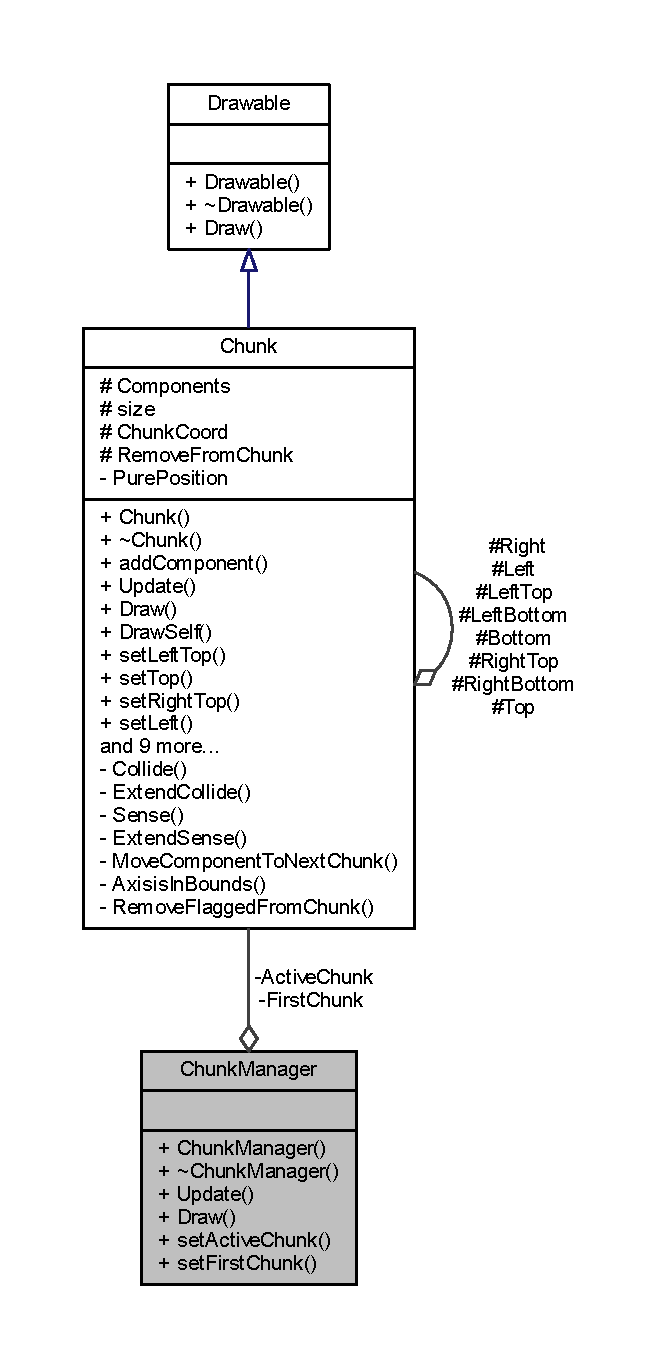
\includegraphics[height=550pt]{class_chunk_manager__coll__graph}
\end{center}
\end{figure}
\subsection*{Public Member Functions}
\begin{DoxyCompactItemize}
\item 
\hyperlink{class_chunk_manager_a5174dca056d736be1e45b71dfc0930ef}{\-\_\-\-\_\-declspec} (dllexport) \hyperlink{class_chunk_manager}{Chunk\-Manager}()
\item 
\hyperlink{class_chunk_manager_a3ea11ca30e6e72f84a1f1bcfe6110543}{\-\_\-\-\_\-declspec} (dllexport)$\sim$\hyperlink{class_chunk_manager}{Chunk\-Manager}()
\item 
\hyperlink{class_chunk_manager_a765c3019448f155961fff4dfeee300ca}{\-\_\-\-\_\-declspec} (dllexport) void Update(const \hyperlink{class_update_data}{Update\-Data} \&updateobject)
\item 
\-\_\-\-\_\-declspec(dllexport) void Draw(sf \hyperlink{class_chunk_manager_a1e77e66b79c2f65848acf922eceebc08}{\-\_\-\-\_\-declspec} (dllexport) void set\-Active\-Chunk(\hyperlink{class_chunk}{Chunk} $\ast$c)
\item 
\hyperlink{class_chunk_manager_aefbc2b592e93d6651226f055eb701d47}{\-\_\-\-\_\-declspec} (dllexport) void set\-First\-Chunk(\hyperlink{class_chunk}{Chunk} $\ast$c)
\item 
\hyperlink{class_chunk_manager_a132a5714695e761d05b32321c721a1d8}{\-\_\-\-\_\-declspec} (dllexport) void add\-Game\-Component(\hyperlink{class_game_component}{Game\-Component} $\ast$c)
\end{DoxyCompactItemize}
\subsection*{Private Attributes}
\begin{DoxyCompactItemize}
\item 
\hyperlink{class_chunk}{Chunk} $\ast$ \hyperlink{class_chunk_manager_a8008f62926fe10f46ac59001aae2d372}{Active\-Chunk}
\item 
\hyperlink{class_chunk}{Chunk} $\ast$ \hyperlink{class_chunk_manager_afb87cd5dd3cb61f09a6038d1796719ba}{First\-Chunk}
\end{DoxyCompactItemize}


\subsection{Member Function Documentation}
\hypertarget{class_chunk_manager_a5174dca056d736be1e45b71dfc0930ef}{\index{Chunk\-Manager@{Chunk\-Manager}!\-\_\-\-\_\-declspec@{\-\_\-\-\_\-declspec}}
\index{\-\_\-\-\_\-declspec@{\-\_\-\-\_\-declspec}!ChunkManager@{Chunk\-Manager}}
\subsubsection[{\-\_\-\-\_\-declspec}]{\setlength{\rightskip}{0pt plus 5cm}Chunk\-Manager\-::\-\_\-\-\_\-declspec (
\begin{DoxyParamCaption}
\item[{dllexport}]{}
\end{DoxyParamCaption}
)}}\label{class_chunk_manager_a5174dca056d736be1e45b71dfc0930ef}
\hypertarget{class_chunk_manager_a3ea11ca30e6e72f84a1f1bcfe6110543}{\index{Chunk\-Manager@{Chunk\-Manager}!\-\_\-\-\_\-declspec@{\-\_\-\-\_\-declspec}}
\index{\-\_\-\-\_\-declspec@{\-\_\-\-\_\-declspec}!ChunkManager@{Chunk\-Manager}}
\subsubsection[{\-\_\-\-\_\-declspec}]{\setlength{\rightskip}{0pt plus 5cm}Chunk\-Manager\-::\-\_\-\-\_\-declspec (
\begin{DoxyParamCaption}
\item[{dllexport}]{}
\end{DoxyParamCaption}
)}}\label{class_chunk_manager_a3ea11ca30e6e72f84a1f1bcfe6110543}
\hypertarget{class_chunk_manager_a765c3019448f155961fff4dfeee300ca}{\index{Chunk\-Manager@{Chunk\-Manager}!\-\_\-\-\_\-declspec@{\-\_\-\-\_\-declspec}}
\index{\-\_\-\-\_\-declspec@{\-\_\-\-\_\-declspec}!ChunkManager@{Chunk\-Manager}}
\subsubsection[{\-\_\-\-\_\-declspec}]{\setlength{\rightskip}{0pt plus 5cm}Chunk\-Manager\-::\-\_\-\-\_\-declspec (
\begin{DoxyParamCaption}
\item[{dllexport}]{}
\end{DoxyParamCaption}
) const}}\label{class_chunk_manager_a765c3019448f155961fff4dfeee300ca}
\hypertarget{class_chunk_manager_a1e77e66b79c2f65848acf922eceebc08}{\index{Chunk\-Manager@{Chunk\-Manager}!\-\_\-\-\_\-declspec@{\-\_\-\-\_\-declspec}}
\index{\-\_\-\-\_\-declspec@{\-\_\-\-\_\-declspec}!ChunkManager@{Chunk\-Manager}}
\subsubsection[{\-\_\-\-\_\-declspec}]{\setlength{\rightskip}{0pt plus 5cm}\-\_\-\-\_\-declspec (dllexport) void Draw(sf Chunk\-Manager\-::\-\_\-\-\_\-declspec (
\begin{DoxyParamCaption}
\item[{dllexport}]{}
\end{DoxyParamCaption}
)}}\label{class_chunk_manager_a1e77e66b79c2f65848acf922eceebc08}
\hypertarget{class_chunk_manager_aefbc2b592e93d6651226f055eb701d47}{\index{Chunk\-Manager@{Chunk\-Manager}!\-\_\-\-\_\-declspec@{\-\_\-\-\_\-declspec}}
\index{\-\_\-\-\_\-declspec@{\-\_\-\-\_\-declspec}!ChunkManager@{Chunk\-Manager}}
\subsubsection[{\-\_\-\-\_\-declspec}]{\setlength{\rightskip}{0pt plus 5cm}Chunk\-Manager\-::\-\_\-\-\_\-declspec (
\begin{DoxyParamCaption}
\item[{dllexport}]{}
\end{DoxyParamCaption}
)}}\label{class_chunk_manager_aefbc2b592e93d6651226f055eb701d47}
\hypertarget{class_chunk_manager_a132a5714695e761d05b32321c721a1d8}{\index{Chunk\-Manager@{Chunk\-Manager}!\-\_\-\-\_\-declspec@{\-\_\-\-\_\-declspec}}
\index{\-\_\-\-\_\-declspec@{\-\_\-\-\_\-declspec}!ChunkManager@{Chunk\-Manager}}
\subsubsection[{\-\_\-\-\_\-declspec}]{\setlength{\rightskip}{0pt plus 5cm}Chunk\-Manager\-::\-\_\-\-\_\-declspec (
\begin{DoxyParamCaption}
\item[{dllexport}]{}
\end{DoxyParamCaption}
)}}\label{class_chunk_manager_a132a5714695e761d05b32321c721a1d8}


\subsection{Member Data Documentation}
\hypertarget{class_chunk_manager_a8008f62926fe10f46ac59001aae2d372}{\index{Chunk\-Manager@{Chunk\-Manager}!Active\-Chunk@{Active\-Chunk}}
\index{Active\-Chunk@{Active\-Chunk}!ChunkManager@{Chunk\-Manager}}
\subsubsection[{Active\-Chunk}]{\setlength{\rightskip}{0pt plus 5cm}{\bf Chunk}$\ast$ Chunk\-Manager\-::\-Active\-Chunk\hspace{0.3cm}{\ttfamily [private]}}}\label{class_chunk_manager_a8008f62926fe10f46ac59001aae2d372}
\hypertarget{class_chunk_manager_afb87cd5dd3cb61f09a6038d1796719ba}{\index{Chunk\-Manager@{Chunk\-Manager}!First\-Chunk@{First\-Chunk}}
\index{First\-Chunk@{First\-Chunk}!ChunkManager@{Chunk\-Manager}}
\subsubsection[{First\-Chunk}]{\setlength{\rightskip}{0pt plus 5cm}{\bf Chunk}$\ast$ Chunk\-Manager\-::\-First\-Chunk\hspace{0.3cm}{\ttfamily [private]}}}\label{class_chunk_manager_afb87cd5dd3cb61f09a6038d1796719ba}


The documentation for this class was generated from the following file\-:\begin{DoxyCompactItemize}
\item 
D\-:/\-Users/tom/\-Documents/\-Visual Studio 2013/\-Projects/\-Revelatorframework/\-Revelator\-Framework\-\_\-\-A\-P\-I/\hyperlink{_chunk_manager_8hpp}{Chunk\-Manager.\-hpp}\end{DoxyCompactItemize}

\hypertarget{class_collidable}{\section{Collidable Class Reference}
\label{class_collidable}\index{Collidable@{Collidable}}
}


{\ttfamily \#include $<$Collidable.\-hpp$>$}



Inheritance diagram for Collidable\-:
\nopagebreak
\begin{figure}[H]
\begin{center}
\leavevmode
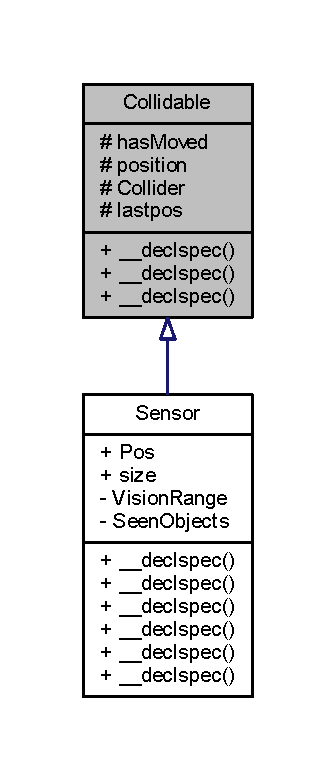
\includegraphics[width=188pt]{class_collidable__inherit__graph}
\end{center}
\end{figure}


Collaboration diagram for Collidable\-:\nopagebreak
\begin{figure}[H]
\begin{center}
\leavevmode
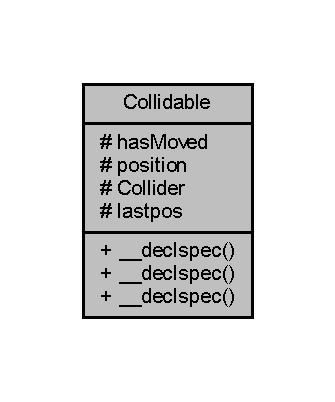
\includegraphics[width=166pt]{class_collidable__coll__graph}
\end{center}
\end{figure}
\subsection*{Public Member Functions}
\begin{DoxyCompactItemize}
\item 
\hyperlink{class_collidable_a92ce9e2b08086bb2f466168ffc69c9ed}{Collidable} ()
\item 
\hyperlink{class_collidable_a71a242ba63c157ca40acbf4421c0eaf7}{Collidable} (sf\-::\-Vector2f $\ast$\hyperlink{class_collidable_aa6c2e113d920df8c0d5da2a244f924bd}{position}, sf\-::\-Vector2f size)
\item 
\hyperlink{class_collidable_a454ca1b66dd504b25fed3706914cee6e}{$\sim$\-Collidable} ()
\item 
\hyperlink{class_rectangle}{Rectangle} \& \hyperlink{class_collidable_ac9edfccd8c5a1ea77238c0a19aa910c3}{get\-Collider} ()
\item 
bool \hyperlink{class_collidable_a8cc1f09ce02e6fcf56d98f07f908a104}{is\-Moved} ()
\end{DoxyCompactItemize}
\subsection*{Protected Attributes}
\begin{DoxyCompactItemize}
\item 
bool \hyperlink{class_collidable_afe5442fd3a82abe62b95e93248d5f4a1}{has\-Moved}
\item 
sf\-::\-Vector2f $\ast$ \hyperlink{class_collidable_aa6c2e113d920df8c0d5da2a244f924bd}{position}
\item 
\hyperlink{class_rectangle}{Rectangle} \hyperlink{class_collidable_a0a81575218d87940935d70800f7d663e}{Collider}
\item 
sf\-::\-Vector2f \hyperlink{class_collidable_ae50dbf8f9d1f584d3a5d5c3445fbe786}{lastpos}
\end{DoxyCompactItemize}


\subsection{Constructor \& Destructor Documentation}
\hypertarget{class_collidable_a92ce9e2b08086bb2f466168ffc69c9ed}{\index{Collidable@{Collidable}!Collidable@{Collidable}}
\index{Collidable@{Collidable}!Collidable@{Collidable}}
\subsubsection[{Collidable}]{\setlength{\rightskip}{0pt plus 5cm}Collidable\-::\-Collidable (
\begin{DoxyParamCaption}
{}
\end{DoxyParamCaption}
)}}\label{class_collidable_a92ce9e2b08086bb2f466168ffc69c9ed}
\hypertarget{class_collidable_a71a242ba63c157ca40acbf4421c0eaf7}{\index{Collidable@{Collidable}!Collidable@{Collidable}}
\index{Collidable@{Collidable}!Collidable@{Collidable}}
\subsubsection[{Collidable}]{\setlength{\rightskip}{0pt plus 5cm}Collidable\-::\-Collidable (
\begin{DoxyParamCaption}
\item[{sf\-::\-Vector2f $\ast$}]{position, }
\item[{sf\-::\-Vector2f}]{size}
\end{DoxyParamCaption}
)}}\label{class_collidable_a71a242ba63c157ca40acbf4421c0eaf7}
\hypertarget{class_collidable_a454ca1b66dd504b25fed3706914cee6e}{\index{Collidable@{Collidable}!$\sim$\-Collidable@{$\sim$\-Collidable}}
\index{$\sim$\-Collidable@{$\sim$\-Collidable}!Collidable@{Collidable}}
\subsubsection[{$\sim$\-Collidable}]{\setlength{\rightskip}{0pt plus 5cm}Collidable\-::$\sim$\-Collidable (
\begin{DoxyParamCaption}
{}
\end{DoxyParamCaption}
)}}\label{class_collidable_a454ca1b66dd504b25fed3706914cee6e}


\subsection{Member Function Documentation}
\hypertarget{class_collidable_ac9edfccd8c5a1ea77238c0a19aa910c3}{\index{Collidable@{Collidable}!get\-Collider@{get\-Collider}}
\index{get\-Collider@{get\-Collider}!Collidable@{Collidable}}
\subsubsection[{get\-Collider}]{\setlength{\rightskip}{0pt plus 5cm}{\bf Rectangle} \& Collidable\-::get\-Collider (
\begin{DoxyParamCaption}
{}
\end{DoxyParamCaption}
)}}\label{class_collidable_ac9edfccd8c5a1ea77238c0a19aa910c3}


Here is the caller graph for this function\-:
\nopagebreak
\begin{figure}[H]
\begin{center}
\leavevmode
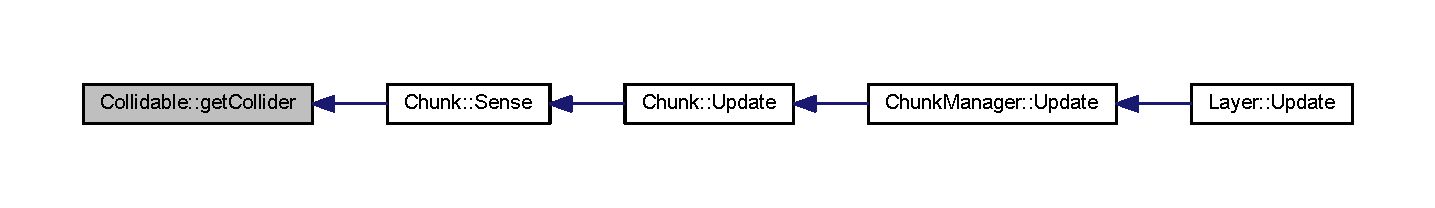
\includegraphics[width=350pt]{class_collidable_ac9edfccd8c5a1ea77238c0a19aa910c3_icgraph}
\end{center}
\end{figure}


\hypertarget{class_collidable_a8cc1f09ce02e6fcf56d98f07f908a104}{\index{Collidable@{Collidable}!is\-Moved@{is\-Moved}}
\index{is\-Moved@{is\-Moved}!Collidable@{Collidable}}
\subsubsection[{is\-Moved}]{\setlength{\rightskip}{0pt plus 5cm}bool Collidable\-::is\-Moved (
\begin{DoxyParamCaption}
{}
\end{DoxyParamCaption}
)}}\label{class_collidable_a8cc1f09ce02e6fcf56d98f07f908a104}


\subsection{Member Data Documentation}
\hypertarget{class_collidable_a0a81575218d87940935d70800f7d663e}{\index{Collidable@{Collidable}!Collider@{Collider}}
\index{Collider@{Collider}!Collidable@{Collidable}}
\subsubsection[{Collider}]{\setlength{\rightskip}{0pt plus 5cm}{\bf Rectangle} Collidable\-::\-Collider\hspace{0.3cm}{\ttfamily [protected]}}}\label{class_collidable_a0a81575218d87940935d70800f7d663e}
\hypertarget{class_collidable_afe5442fd3a82abe62b95e93248d5f4a1}{\index{Collidable@{Collidable}!has\-Moved@{has\-Moved}}
\index{has\-Moved@{has\-Moved}!Collidable@{Collidable}}
\subsubsection[{has\-Moved}]{\setlength{\rightskip}{0pt plus 5cm}bool Collidable\-::has\-Moved\hspace{0.3cm}{\ttfamily [protected]}}}\label{class_collidable_afe5442fd3a82abe62b95e93248d5f4a1}
\hypertarget{class_collidable_ae50dbf8f9d1f584d3a5d5c3445fbe786}{\index{Collidable@{Collidable}!lastpos@{lastpos}}
\index{lastpos@{lastpos}!Collidable@{Collidable}}
\subsubsection[{lastpos}]{\setlength{\rightskip}{0pt plus 5cm}sf\-::\-Vector2f Collidable\-::lastpos\hspace{0.3cm}{\ttfamily [protected]}}}\label{class_collidable_ae50dbf8f9d1f584d3a5d5c3445fbe786}
\hypertarget{class_collidable_aa6c2e113d920df8c0d5da2a244f924bd}{\index{Collidable@{Collidable}!position@{position}}
\index{position@{position}!Collidable@{Collidable}}
\subsubsection[{position}]{\setlength{\rightskip}{0pt plus 5cm}sf\-::\-Vector2f$\ast$ Collidable\-::position\hspace{0.3cm}{\ttfamily [protected]}}}\label{class_collidable_aa6c2e113d920df8c0d5da2a244f924bd}


The documentation for this class was generated from the following files\-:\begin{DoxyCompactItemize}
\item 
D\-:/\-Users/tom/\-Documents/\-Visual Studio 2013/\-Projects/\-Revelatorframework/\-Revelatorframework/\hyperlink{_collidable_8hpp}{Collidable.\-hpp}\item 
D\-:/\-Users/tom/\-Documents/\-Visual Studio 2013/\-Projects/\-Revelatorframework/\-Revelatorframework/\hyperlink{_collidable_8cpp}{Collidable.\-cpp}\end{DoxyCompactItemize}

\hypertarget{class_drawable}{\section{Drawable Class Reference}
\label{class_drawable}\index{Drawable@{Drawable}}
}


{\ttfamily \#include $<$Drawable.\-hpp$>$}



Inheritance diagram for Drawable\-:
\nopagebreak
\begin{figure}[H]
\begin{center}
\leavevmode
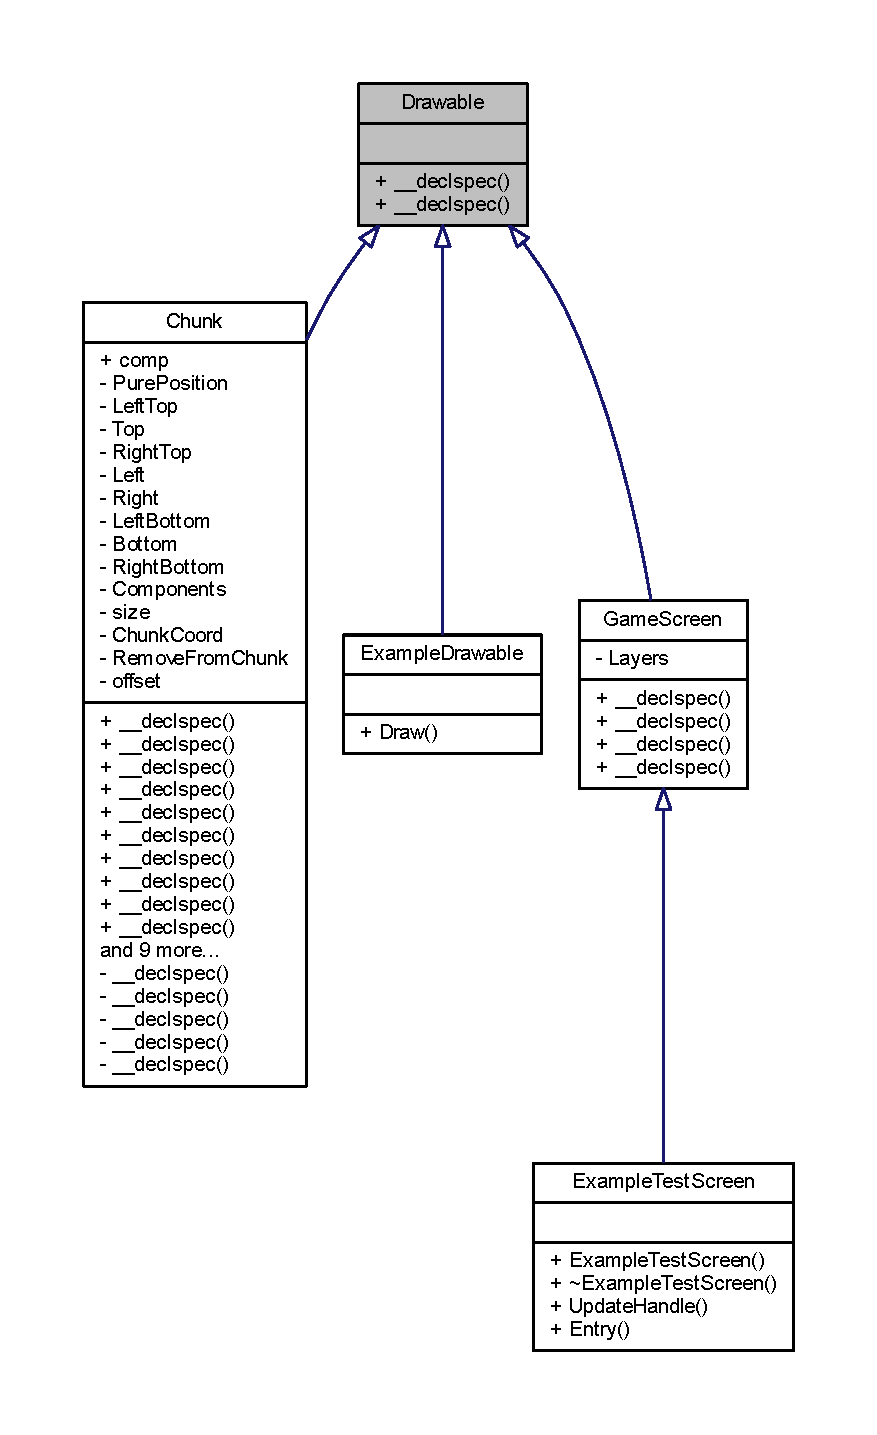
\includegraphics[height=550pt]{class_drawable__inherit__graph}
\end{center}
\end{figure}


Collaboration diagram for Drawable\-:\nopagebreak
\begin{figure}[H]
\begin{center}
\leavevmode
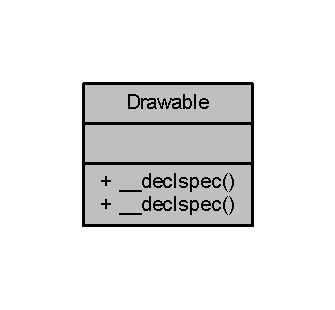
\includegraphics[width=161pt]{class_drawable__coll__graph}
\end{center}
\end{figure}
\subsection*{Public Member Functions}
\begin{DoxyCompactItemize}
\item 
\hyperlink{class_drawable_ac9f04cf11a84eb3cdf68ea48599648d7}{\-\_\-\-\_\-declspec} (dllexport) \hyperlink{class_drawable}{Drawable}()
\item 
\hyperlink{class_drawable_ab8175a6d9337a90bd36e368bd6749579}{\-\_\-\-\_\-declspec} (dllexport)$\sim$\hyperlink{class_drawable}{Drawable}()
\end{DoxyCompactItemize}


\subsection{Member Function Documentation}
\hypertarget{class_drawable_ac9f04cf11a84eb3cdf68ea48599648d7}{\index{Drawable@{Drawable}!\-\_\-\-\_\-declspec@{\-\_\-\-\_\-declspec}}
\index{\-\_\-\-\_\-declspec@{\-\_\-\-\_\-declspec}!Drawable@{Drawable}}
\subsubsection[{\-\_\-\-\_\-declspec}]{\setlength{\rightskip}{0pt plus 5cm}Drawable\-::\-\_\-\-\_\-declspec (
\begin{DoxyParamCaption}
\item[{dllexport}]{}
\end{DoxyParamCaption}
)}}\label{class_drawable_ac9f04cf11a84eb3cdf68ea48599648d7}
\hypertarget{class_drawable_ab8175a6d9337a90bd36e368bd6749579}{\index{Drawable@{Drawable}!\-\_\-\-\_\-declspec@{\-\_\-\-\_\-declspec}}
\index{\-\_\-\-\_\-declspec@{\-\_\-\-\_\-declspec}!Drawable@{Drawable}}
\subsubsection[{\-\_\-\-\_\-declspec}]{\setlength{\rightskip}{0pt plus 5cm}Drawable\-::\-\_\-\-\_\-declspec (
\begin{DoxyParamCaption}
\item[{dllexport}]{}
\end{DoxyParamCaption}
)}}\label{class_drawable_ab8175a6d9337a90bd36e368bd6749579}


The documentation for this class was generated from the following file\-:\begin{DoxyCompactItemize}
\item 
D\-:/\-Users/tom/\-Documents/\-Visual Studio 2013/\-Projects/\-Revelatorframework/\-Revelator\-Framework\-\_\-\-A\-P\-I/\hyperlink{_drawable_8hpp}{Drawable.\-hpp}\end{DoxyCompactItemize}

\hypertarget{class_entry_object}{\section{Entry\-Object Class Reference}
\label{class_entry_object}\index{Entry\-Object@{Entry\-Object}}
}


{\ttfamily \#include $<$Entry\-Object.\-hpp$>$}



Collaboration diagram for Entry\-Object\-:\nopagebreak
\begin{figure}[H]
\begin{center}
\leavevmode
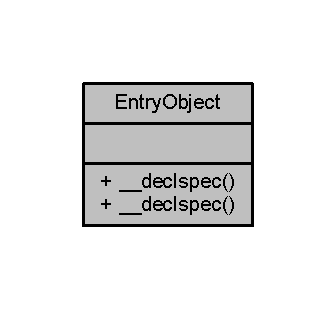
\includegraphics[width=169pt]{class_entry_object__coll__graph}
\end{center}
\end{figure}
\subsection*{Public Member Functions}
\begin{DoxyCompactItemize}
\item 
\hyperlink{class_entry_object_a96dedc7047bc1d962022c91118aedc14}{Entry\-Object} ()
\begin{DoxyCompactList}\small\item\em The default constructor. \end{DoxyCompactList}\item 
\hyperlink{class_entry_object_a5b6738e8fb3c234df0f24b02f21dea53}{$\sim$\-Entry\-Object} ()
\begin{DoxyCompactList}\small\item\em The destructor. \end{DoxyCompactList}\end{DoxyCompactItemize}


\subsection{Constructor \& Destructor Documentation}
\hypertarget{class_entry_object_a96dedc7047bc1d962022c91118aedc14}{\index{Entry\-Object@{Entry\-Object}!Entry\-Object@{Entry\-Object}}
\index{Entry\-Object@{Entry\-Object}!EntryObject@{Entry\-Object}}
\subsubsection[{Entry\-Object}]{\setlength{\rightskip}{0pt plus 5cm}Entry\-Object\-::\-Entry\-Object (
\begin{DoxyParamCaption}
{}
\end{DoxyParamCaption}
)}}\label{class_entry_object_a96dedc7047bc1d962022c91118aedc14}


The default constructor. 

\hypertarget{class_entry_object_a5b6738e8fb3c234df0f24b02f21dea53}{\index{Entry\-Object@{Entry\-Object}!$\sim$\-Entry\-Object@{$\sim$\-Entry\-Object}}
\index{$\sim$\-Entry\-Object@{$\sim$\-Entry\-Object}!EntryObject@{Entry\-Object}}
\subsubsection[{$\sim$\-Entry\-Object}]{\setlength{\rightskip}{0pt plus 5cm}Entry\-Object\-::$\sim$\-Entry\-Object (
\begin{DoxyParamCaption}
{}
\end{DoxyParamCaption}
)}}\label{class_entry_object_a5b6738e8fb3c234df0f24b02f21dea53}


The destructor. 



The documentation for this class was generated from the following files\-:\begin{DoxyCompactItemize}
\item 
D\-:/\-Users/tom/\-Documents/\-Visual Studio 2013/\-Projects/\-Revelatorframework/\-Revelator\-Framework\-\_\-\-A\-P\-I/\hyperlink{_entry_object_8hpp}{Entry\-Object.\-hpp}\item 
D\-:/\-Users/tom/\-Documents/\-Visual Studio 2013/\-Projects/\-Revelatorframework/\-Revelator\-Framework\-\_\-\-A\-P\-I/\hyperlink{_entry_object_8cpp}{Entry\-Object.\-cpp}\end{DoxyCompactItemize}

\hypertarget{class_example_component}{\section{Example\-Component Class Reference}
\label{class_example_component}\index{Example\-Component@{Example\-Component}}
}


{\ttfamily \#include $<$Example\-Component.\-hpp$>$}



Inheritance diagram for Example\-Component\-:\nopagebreak
\begin{figure}[H]
\begin{center}
\leavevmode
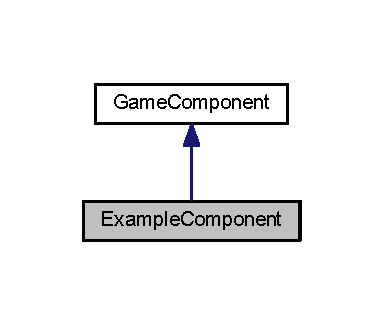
\includegraphics[width=205pt]{class_example_component__inherit__graph}
\end{center}
\end{figure}


Collaboration diagram for Example\-Component\-:
\nopagebreak
\begin{figure}[H]
\begin{center}
\leavevmode
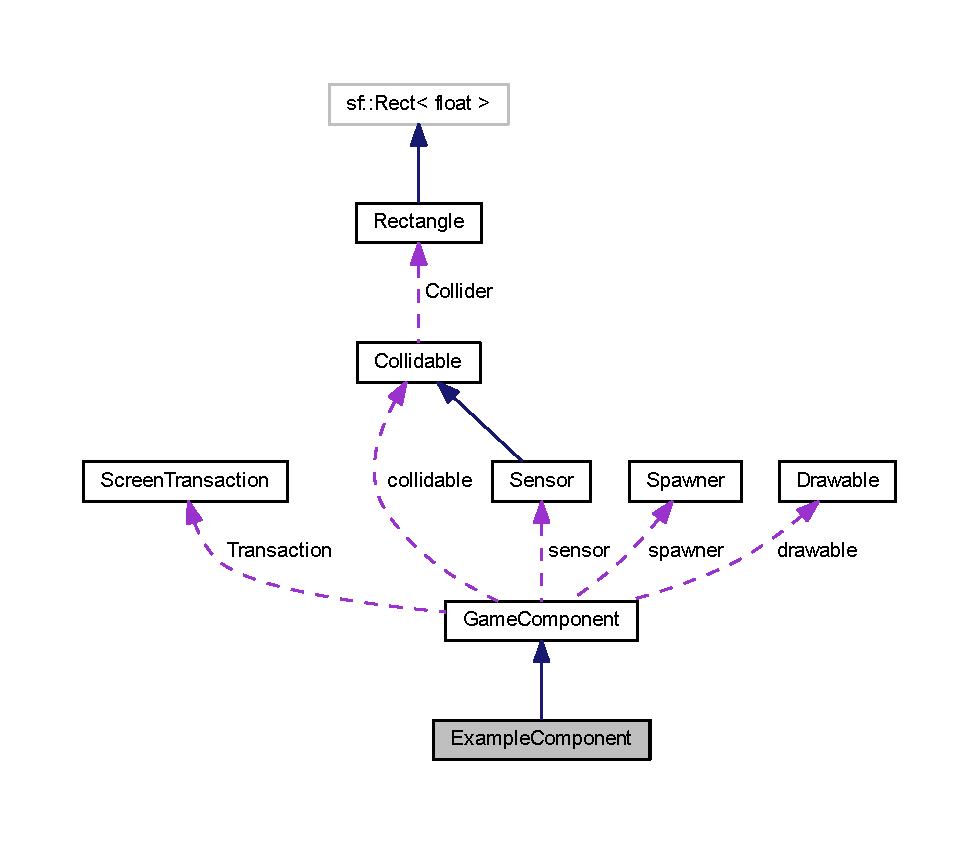
\includegraphics[width=350pt]{class_example_component__coll__graph}
\end{center}
\end{figure}
\subsection*{Public Member Functions}
\begin{DoxyCompactItemize}
\item 
\hyperlink{class_example_component_a09d97ad014e5ebe38220da6c80e96873}{Example\-Component} (sf\-::\-Vector2f pos=sf\-::\-Vector2f\{0.f, 0.f\})
\item 
void \hyperlink{class_example_component_a6ab733042d45aaa046201f486ece06b5}{Collide} (\hyperlink{class_game_component}{Game\-Component} $\ast$colider) override
\item 
\hyperlink{class_example_component_aa3a6265806020d1536d21272906181c6}{$\sim$\-Example\-Component} ()
\item 
void \hyperlink{class_example_component_a74028c9fbf9ec0fc523e60416433eacb}{Update} (\hyperlink{class_update_data}{Update\-Data} $\ast$updateobject) override
\item 
void \hyperlink{class_example_component_a385a5f04cdf04e91c8340632a1af9edc}{Draw} (sf\-::\-Render\-Window \&window, sf\-::\-Vector2f offset)
\end{DoxyCompactItemize}
\subsection*{Additional Inherited Members}


\subsection{Constructor \& Destructor Documentation}
\hypertarget{class_example_component_a09d97ad014e5ebe38220da6c80e96873}{\index{Example\-Component@{Example\-Component}!Example\-Component@{Example\-Component}}
\index{Example\-Component@{Example\-Component}!ExampleComponent@{Example\-Component}}
\subsubsection[{Example\-Component}]{\setlength{\rightskip}{0pt plus 5cm}Example\-Component\-::\-Example\-Component (
\begin{DoxyParamCaption}
\item[{sf\-::\-Vector2f}]{pos = {\ttfamily sf\-:\-:Vector2f\{0.f,0.f\}}}
\end{DoxyParamCaption}
)}}\label{class_example_component_a09d97ad014e5ebe38220da6c80e96873}
\hypertarget{class_example_component_aa3a6265806020d1536d21272906181c6}{\index{Example\-Component@{Example\-Component}!$\sim$\-Example\-Component@{$\sim$\-Example\-Component}}
\index{$\sim$\-Example\-Component@{$\sim$\-Example\-Component}!ExampleComponent@{Example\-Component}}
\subsubsection[{$\sim$\-Example\-Component}]{\setlength{\rightskip}{0pt plus 5cm}Example\-Component\-::$\sim$\-Example\-Component (
\begin{DoxyParamCaption}
{}
\end{DoxyParamCaption}
)}}\label{class_example_component_aa3a6265806020d1536d21272906181c6}


\subsection{Member Function Documentation}
\hypertarget{class_example_component_a6ab733042d45aaa046201f486ece06b5}{\index{Example\-Component@{Example\-Component}!Collide@{Collide}}
\index{Collide@{Collide}!ExampleComponent@{Example\-Component}}
\subsubsection[{Collide}]{\setlength{\rightskip}{0pt plus 5cm}void Example\-Component\-::\-Collide (
\begin{DoxyParamCaption}
\item[{{\bf Game\-Component} $\ast$}]{colider}
\end{DoxyParamCaption}
)\hspace{0.3cm}{\ttfamily [override]}}}\label{class_example_component_a6ab733042d45aaa046201f486ece06b5}
\hypertarget{class_example_component_a385a5f04cdf04e91c8340632a1af9edc}{\index{Example\-Component@{Example\-Component}!Draw@{Draw}}
\index{Draw@{Draw}!ExampleComponent@{Example\-Component}}
\subsubsection[{Draw}]{\setlength{\rightskip}{0pt plus 5cm}void Example\-Component\-::\-Draw (
\begin{DoxyParamCaption}
\item[{sf\-::\-Render\-Window \&}]{window, }
\item[{sf\-::\-Vector2f}]{offset}
\end{DoxyParamCaption}
)}}\label{class_example_component_a385a5f04cdf04e91c8340632a1af9edc}
\hypertarget{class_example_component_a74028c9fbf9ec0fc523e60416433eacb}{\index{Example\-Component@{Example\-Component}!Update@{Update}}
\index{Update@{Update}!ExampleComponent@{Example\-Component}}
\subsubsection[{Update}]{\setlength{\rightskip}{0pt plus 5cm}void Example\-Component\-::\-Update (
\begin{DoxyParamCaption}
\item[{{\bf Update\-Data} $\ast$}]{updateobject}
\end{DoxyParamCaption}
)\hspace{0.3cm}{\ttfamily [override]}}}\label{class_example_component_a74028c9fbf9ec0fc523e60416433eacb}


The documentation for this class was generated from the following files\-:\begin{DoxyCompactItemize}
\item 
D\-:/\-Users/tom/\-Documents/\-Visual Studio 2013/\-Projects/\-Revelatorframework/\-Revelatorframework/\hyperlink{_example_component_8hpp}{Example\-Component.\-hpp}\item 
D\-:/\-Users/tom/\-Documents/\-Visual Studio 2013/\-Projects/\-Revelatorframework/\-Revelatorframework/\hyperlink{_example_component_8cpp}{Example\-Component.\-cpp}\end{DoxyCompactItemize}

\hypertarget{class_example_component_producer}{\section{Example\-Component\-Producer Class Reference}
\label{class_example_component_producer}\index{Example\-Component\-Producer@{Example\-Component\-Producer}}
}


{\ttfamily \#include $<$Example\-Component\-Producer.\-hpp$>$}



Inheritance diagram for Example\-Component\-Producer\-:\nopagebreak
\begin{figure}[H]
\begin{center}
\leavevmode
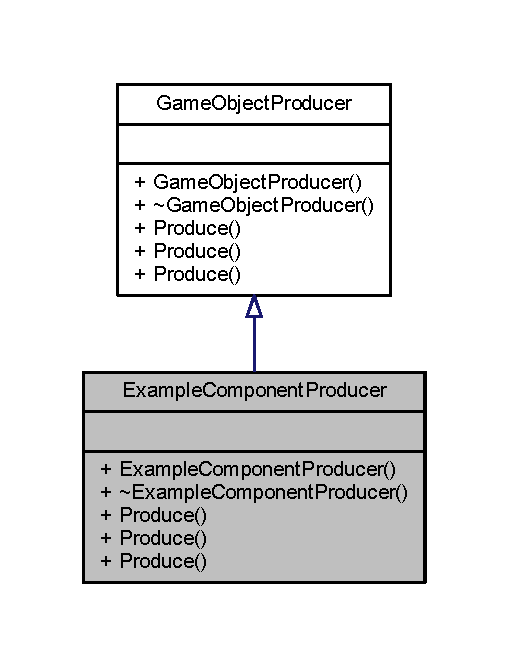
\includegraphics[width=244pt]{class_example_component_producer__inherit__graph}
\end{center}
\end{figure}


Collaboration diagram for Example\-Component\-Producer\-:\nopagebreak
\begin{figure}[H]
\begin{center}
\leavevmode
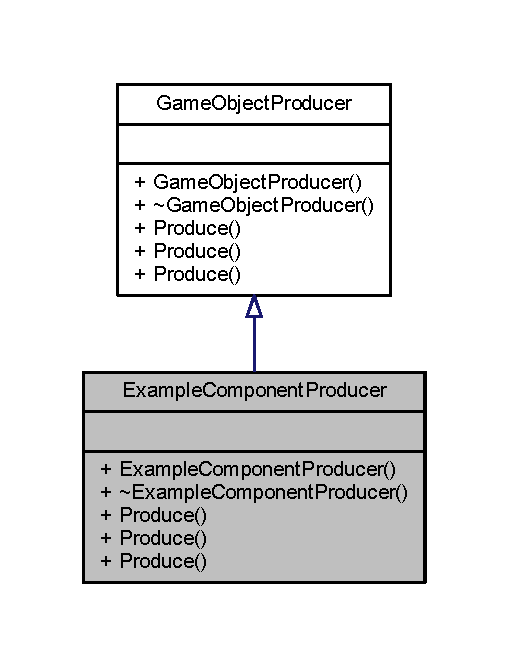
\includegraphics[width=244pt]{class_example_component_producer__coll__graph}
\end{center}
\end{figure}
\subsection*{Public Member Functions}
\begin{DoxyCompactItemize}
\item 
\hyperlink{class_example_component_producer_ad4eeb56b75cbf68545d82619aa8e0184}{Example\-Component\-Producer} ()
\item 
\hyperlink{class_example_component_producer_a2c090cf13157589dfcd4fd9441d4d4f3}{$\sim$\-Example\-Component\-Producer} ()
\item 
\hyperlink{class_game_component}{Game\-Component} $\ast$ \hyperlink{class_example_component_producer_a63aba60e4b967000da407340505838de}{Produce} ()
\item 
\hyperlink{class_game_component}{Game\-Component} $\ast$ \hyperlink{class_example_component_producer_aeb985b69039c1db83c5826c01f31f53c}{Produce} (\hyperlink{class_producer_package}{Producer\-Package} Package)
\item 
\hyperlink{class_game_component}{Game\-Component} $\ast$ \hyperlink{class_example_component_producer_a177b5d9088f69aed43d10c9b2b8f2c01}{Produce} (\hyperlink{class_producer_package}{Producer\-Package} $\ast$Package)
\end{DoxyCompactItemize}


\subsection{Constructor \& Destructor Documentation}
\hypertarget{class_example_component_producer_ad4eeb56b75cbf68545d82619aa8e0184}{\index{Example\-Component\-Producer@{Example\-Component\-Producer}!Example\-Component\-Producer@{Example\-Component\-Producer}}
\index{Example\-Component\-Producer@{Example\-Component\-Producer}!ExampleComponentProducer@{Example\-Component\-Producer}}
\subsubsection[{Example\-Component\-Producer}]{\setlength{\rightskip}{0pt plus 5cm}Example\-Component\-Producer\-::\-Example\-Component\-Producer (
\begin{DoxyParamCaption}
{}
\end{DoxyParamCaption}
)}}\label{class_example_component_producer_ad4eeb56b75cbf68545d82619aa8e0184}
\hypertarget{class_example_component_producer_a2c090cf13157589dfcd4fd9441d4d4f3}{\index{Example\-Component\-Producer@{Example\-Component\-Producer}!$\sim$\-Example\-Component\-Producer@{$\sim$\-Example\-Component\-Producer}}
\index{$\sim$\-Example\-Component\-Producer@{$\sim$\-Example\-Component\-Producer}!ExampleComponentProducer@{Example\-Component\-Producer}}
\subsubsection[{$\sim$\-Example\-Component\-Producer}]{\setlength{\rightskip}{0pt plus 5cm}Example\-Component\-Producer\-::$\sim$\-Example\-Component\-Producer (
\begin{DoxyParamCaption}
{}
\end{DoxyParamCaption}
)}}\label{class_example_component_producer_a2c090cf13157589dfcd4fd9441d4d4f3}


\subsection{Member Function Documentation}
\hypertarget{class_example_component_producer_a63aba60e4b967000da407340505838de}{\index{Example\-Component\-Producer@{Example\-Component\-Producer}!Produce@{Produce}}
\index{Produce@{Produce}!ExampleComponentProducer@{Example\-Component\-Producer}}
\subsubsection[{Produce}]{\setlength{\rightskip}{0pt plus 5cm}{\bf Game\-Component} $\ast$ Example\-Component\-Producer\-::\-Produce (
\begin{DoxyParamCaption}
{}
\end{DoxyParamCaption}
)}}\label{class_example_component_producer_a63aba60e4b967000da407340505838de}


Here is the caller graph for this function\-:\nopagebreak
\begin{figure}[H]
\begin{center}
\leavevmode
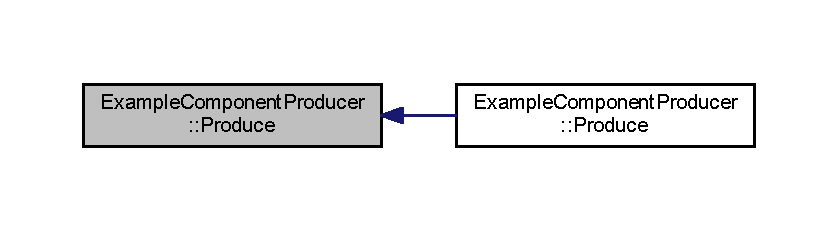
\includegraphics[width=350pt]{class_example_component_producer_a63aba60e4b967000da407340505838de_icgraph}
\end{center}
\end{figure}


\hypertarget{class_example_component_producer_aeb985b69039c1db83c5826c01f31f53c}{\index{Example\-Component\-Producer@{Example\-Component\-Producer}!Produce@{Produce}}
\index{Produce@{Produce}!ExampleComponentProducer@{Example\-Component\-Producer}}
\subsubsection[{Produce}]{\setlength{\rightskip}{0pt plus 5cm}{\bf Game\-Component} $\ast$ Example\-Component\-Producer\-::\-Produce (
\begin{DoxyParamCaption}
\item[{{\bf Producer\-Package}}]{Package}
\end{DoxyParamCaption}
)}}\label{class_example_component_producer_aeb985b69039c1db83c5826c01f31f53c}
\hypertarget{class_example_component_producer_a177b5d9088f69aed43d10c9b2b8f2c01}{\index{Example\-Component\-Producer@{Example\-Component\-Producer}!Produce@{Produce}}
\index{Produce@{Produce}!ExampleComponentProducer@{Example\-Component\-Producer}}
\subsubsection[{Produce}]{\setlength{\rightskip}{0pt plus 5cm}{\bf Game\-Component} $\ast$ Example\-Component\-Producer\-::\-Produce (
\begin{DoxyParamCaption}
\item[{{\bf Producer\-Package} $\ast$}]{Package}
\end{DoxyParamCaption}
)}}\label{class_example_component_producer_a177b5d9088f69aed43d10c9b2b8f2c01}


Here is the call graph for this function\-:\nopagebreak
\begin{figure}[H]
\begin{center}
\leavevmode
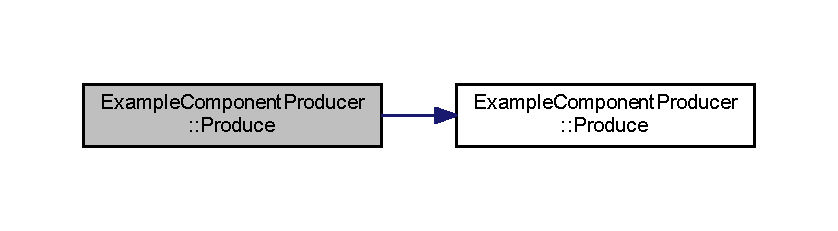
\includegraphics[width=350pt]{class_example_component_producer_a177b5d9088f69aed43d10c9b2b8f2c01_cgraph}
\end{center}
\end{figure}




The documentation for this class was generated from the following files\-:\begin{DoxyCompactItemize}
\item 
D\-:/\-Users/tom/\-Documents/\-Visual Studio 2013/\-Projects/\-Revelatorframework/\-Revelatorframework/\hyperlink{_example_component_producer_8hpp}{Example\-Component\-Producer.\-hpp}\item 
D\-:/\-Users/tom/\-Documents/\-Visual Studio 2013/\-Projects/\-Revelatorframework/\-Revelatorframework/\hyperlink{_example_component_producer_8cpp}{Example\-Component\-Producer.\-cpp}\end{DoxyCompactItemize}

\hypertarget{class_example_drawable}{\section{Example\-Drawable Class Reference}
\label{class_example_drawable}\index{Example\-Drawable@{Example\-Drawable}}
}


{\ttfamily \#include $<$Example\-Component.\-hpp$>$}



Inheritance diagram for Example\-Drawable\-:\nopagebreak
\begin{figure}[H]
\begin{center}
\leavevmode
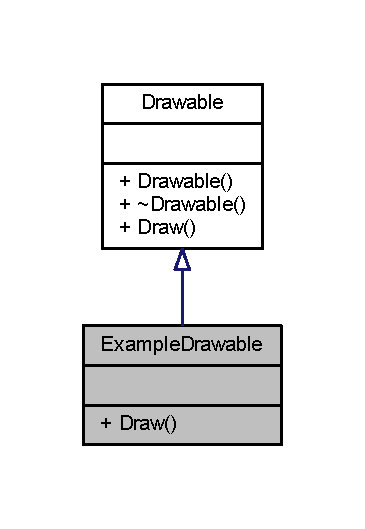
\includegraphics[width=175pt]{class_example_drawable__inherit__graph}
\end{center}
\end{figure}


Collaboration diagram for Example\-Drawable\-:\nopagebreak
\begin{figure}[H]
\begin{center}
\leavevmode
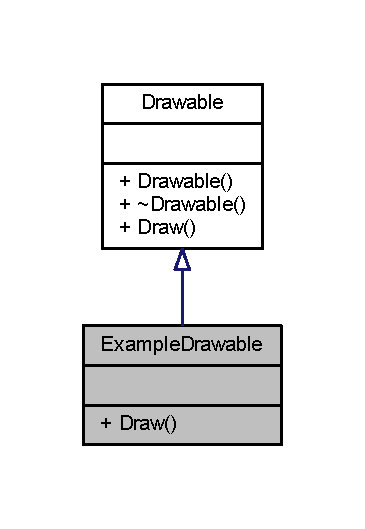
\includegraphics[width=175pt]{class_example_drawable__coll__graph}
\end{center}
\end{figure}
\subsection*{Public Member Functions}
\begin{DoxyCompactItemize}
\item 
void \hyperlink{class_example_drawable_a02efe170a267616262e1bac3d65cdf59}{Draw} (sf\-::\-Render\-Window \&window, sf\-::\-Vector2f offset) override
\end{DoxyCompactItemize}


\subsection{Member Function Documentation}
\hypertarget{class_example_drawable_a02efe170a267616262e1bac3d65cdf59}{\index{Example\-Drawable@{Example\-Drawable}!Draw@{Draw}}
\index{Draw@{Draw}!ExampleDrawable@{Example\-Drawable}}
\subsubsection[{Draw}]{\setlength{\rightskip}{0pt plus 5cm}void Example\-Drawable\-::\-Draw (
\begin{DoxyParamCaption}
\item[{sf\-::\-Render\-Window \&}]{window, }
\item[{sf\-::\-Vector2f}]{offset}
\end{DoxyParamCaption}
)\hspace{0.3cm}{\ttfamily [override]}, {\ttfamily [virtual]}}}\label{class_example_drawable_a02efe170a267616262e1bac3d65cdf59}


Implements \hyperlink{class_drawable_a0e24de52eeb44555872c70f3adf854d2}{Drawable}.



The documentation for this class was generated from the following files\-:\begin{DoxyCompactItemize}
\item 
D\-:/\-Users/tom/\-Documents/\-Visual Studio 2013/\-Projects/\-Revelatorframework/\-Revelatorframework/\hyperlink{_example_component_8hpp}{Example\-Component.\-hpp}\item 
D\-:/\-Users/tom/\-Documents/\-Visual Studio 2013/\-Projects/\-Revelatorframework/\-Revelatorframework/\hyperlink{_example_component_8cpp}{Example\-Component.\-cpp}\end{DoxyCompactItemize}

\hypertarget{class_example_layer}{\section{Example\-Layer Class Reference}
\label{class_example_layer}\index{Example\-Layer@{Example\-Layer}}
}


{\ttfamily \#include $<$Example\-Layer.\-hpp$>$}



Inheritance diagram for Example\-Layer\-:\nopagebreak
\begin{figure}[H]
\begin{center}
\leavevmode
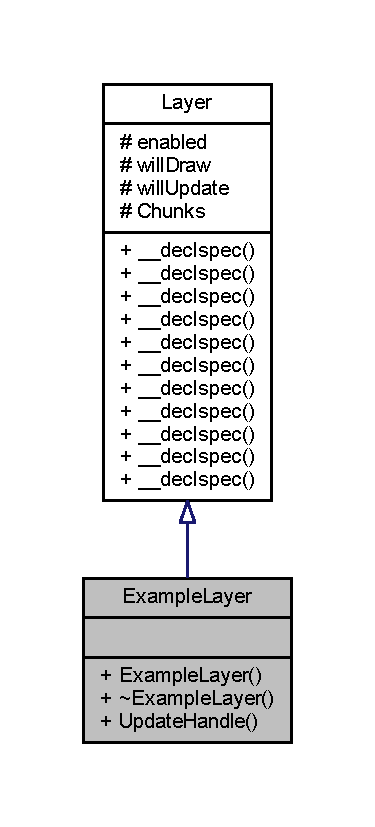
\includegraphics[width=190pt]{class_example_layer__inherit__graph}
\end{center}
\end{figure}


Collaboration diagram for Example\-Layer\-:\nopagebreak
\begin{figure}[H]
\begin{center}
\leavevmode
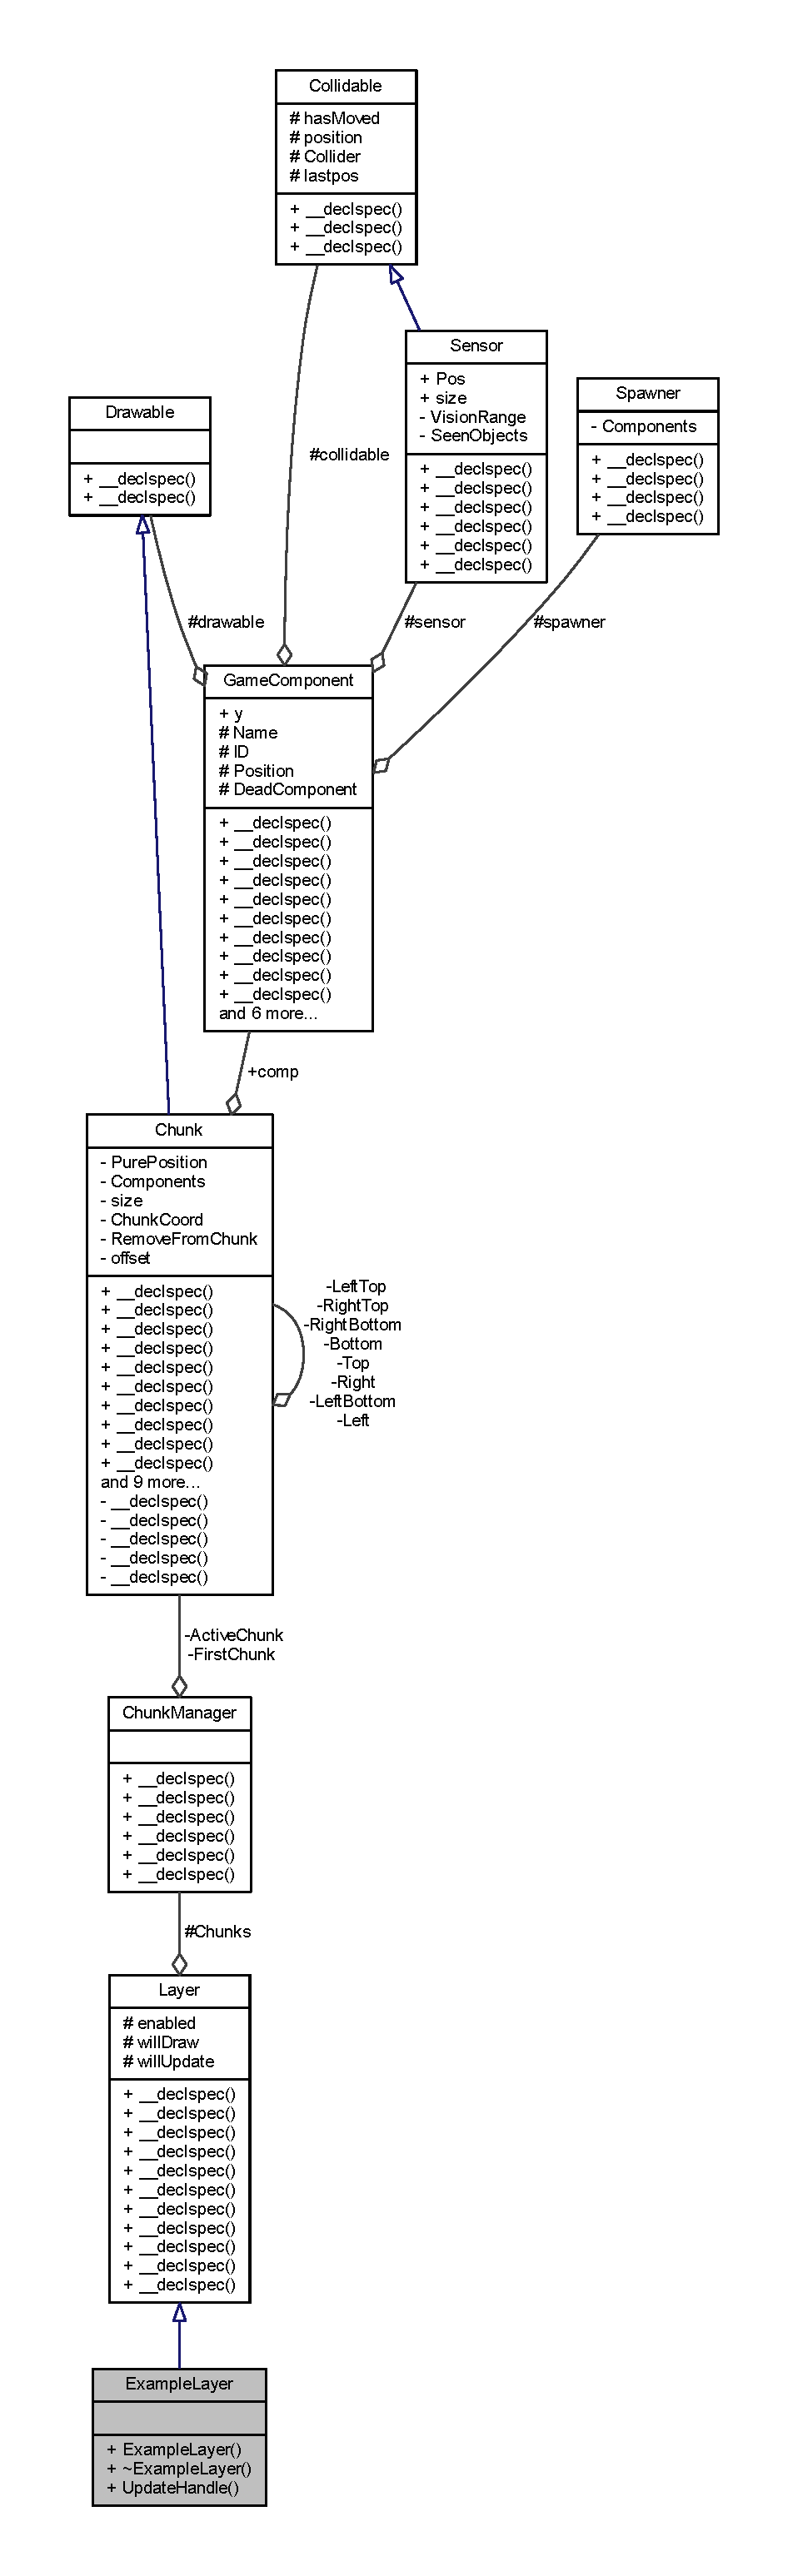
\includegraphics[height=550pt]{class_example_layer__coll__graph}
\end{center}
\end{figure}
\subsection*{Public Member Functions}
\begin{DoxyCompactItemize}
\item 
\hyperlink{class_example_layer_a199ad822f707990b69e998a9ed7df5bb}{Example\-Layer} ()
\item 
\hyperlink{class_example_layer_a243387a90a54149af7d128301e836522}{$\sim$\-Example\-Layer} ()
\item 
void \hyperlink{class_example_layer_a97b36d082a4b5dd7e145773fca666490}{Update\-Handle} (const \hyperlink{class_update_data}{Update\-Data} \&updateobject) override
\end{DoxyCompactItemize}
\subsection*{Additional Inherited Members}


\subsection{Constructor \& Destructor Documentation}
\hypertarget{class_example_layer_a199ad822f707990b69e998a9ed7df5bb}{\index{Example\-Layer@{Example\-Layer}!Example\-Layer@{Example\-Layer}}
\index{Example\-Layer@{Example\-Layer}!ExampleLayer@{Example\-Layer}}
\subsubsection[{Example\-Layer}]{\setlength{\rightskip}{0pt plus 5cm}Example\-Layer\-::\-Example\-Layer (
\begin{DoxyParamCaption}
{}
\end{DoxyParamCaption}
)}}\label{class_example_layer_a199ad822f707990b69e998a9ed7df5bb}
\hypertarget{class_example_layer_a243387a90a54149af7d128301e836522}{\index{Example\-Layer@{Example\-Layer}!$\sim$\-Example\-Layer@{$\sim$\-Example\-Layer}}
\index{$\sim$\-Example\-Layer@{$\sim$\-Example\-Layer}!ExampleLayer@{Example\-Layer}}
\subsubsection[{$\sim$\-Example\-Layer}]{\setlength{\rightskip}{0pt plus 5cm}Example\-Layer\-::$\sim$\-Example\-Layer (
\begin{DoxyParamCaption}
{}
\end{DoxyParamCaption}
)}}\label{class_example_layer_a243387a90a54149af7d128301e836522}


\subsection{Member Function Documentation}
\hypertarget{class_example_layer_a97b36d082a4b5dd7e145773fca666490}{\index{Example\-Layer@{Example\-Layer}!Update\-Handle@{Update\-Handle}}
\index{Update\-Handle@{Update\-Handle}!ExampleLayer@{Example\-Layer}}
\subsubsection[{Update\-Handle}]{\setlength{\rightskip}{0pt plus 5cm}void Example\-Layer\-::\-Update\-Handle (
\begin{DoxyParamCaption}
\item[{const {\bf Update\-Data} \&}]{updateobject}
\end{DoxyParamCaption}
)\hspace{0.3cm}{\ttfamily [inline]}, {\ttfamily [override]}, {\ttfamily [virtual]}}}\label{class_example_layer_a97b36d082a4b5dd7e145773fca666490}


Implements \hyperlink{class_layer_a1e7a6db5ee252c8ea9c44a21aaf2b0c9}{Layer}.



The documentation for this class was generated from the following files\-:\begin{DoxyCompactItemize}
\item 
D\-:/\-Users/tom/\-Documents/\-Visual Studio 2013/\-Projects/\-Revelatorframework/\-Revelatorframework/\hyperlink{_example_layer_8hpp}{Example\-Layer.\-hpp}\item 
D\-:/\-Users/tom/\-Documents/\-Visual Studio 2013/\-Projects/\-Revelatorframework/\-Revelatorframework/\hyperlink{_example_layer_8cpp}{Example\-Layer.\-cpp}\end{DoxyCompactItemize}

\hypertarget{class_example_layer_producer}{\section{Example\-Layer\-Producer Class Reference}
\label{class_example_layer_producer}\index{Example\-Layer\-Producer@{Example\-Layer\-Producer}}
}


{\ttfamily \#include $<$Example\-Layer\-Producer.\-hpp$>$}



Inheritance diagram for Example\-Layer\-Producer\-:\nopagebreak
\begin{figure}[H]
\begin{center}
\leavevmode
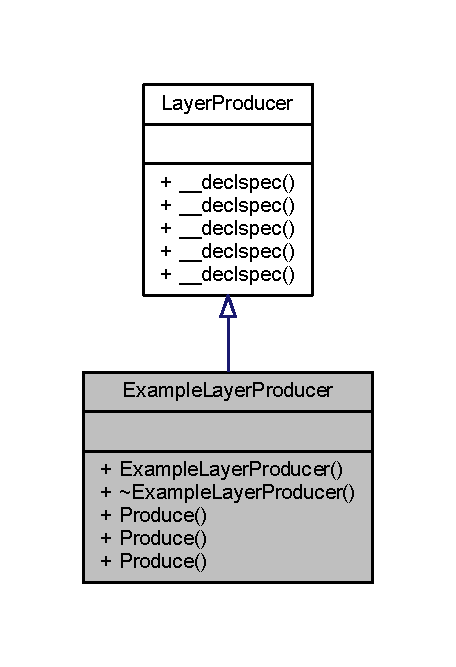
\includegraphics[width=219pt]{class_example_layer_producer__inherit__graph}
\end{center}
\end{figure}


Collaboration diagram for Example\-Layer\-Producer\-:\nopagebreak
\begin{figure}[H]
\begin{center}
\leavevmode
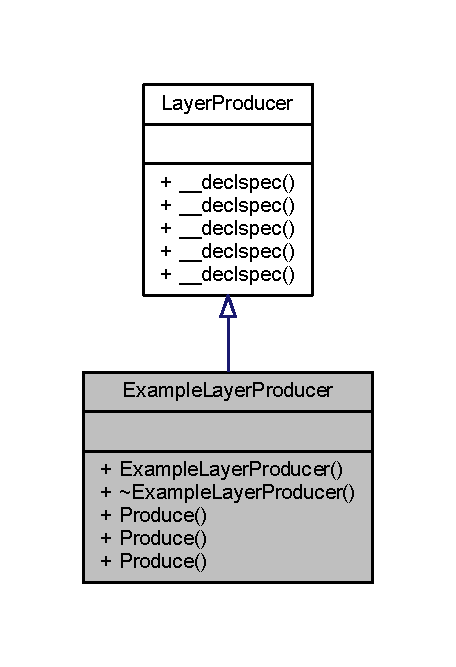
\includegraphics[width=219pt]{class_example_layer_producer__coll__graph}
\end{center}
\end{figure}
\subsection*{Public Member Functions}
\begin{DoxyCompactItemize}
\item 
\hyperlink{class_example_layer_producer_a46734be5040e6cfe596f8f9bfd2703cd}{Example\-Layer\-Producer} ()
\item 
\hyperlink{class_example_layer_producer_a15a878dbc6d3ecf06f5997686b1cb0a6}{$\sim$\-Example\-Layer\-Producer} ()
\item 
\hyperlink{class_layer}{Layer} $\ast$ \hyperlink{class_example_layer_producer_add9cb70333ae10c7a1c58d7e4d8f64fc}{Produce} () override
\item 
\hyperlink{class_layer}{Layer} $\ast$ \hyperlink{class_example_layer_producer_adb3d15b45aeaaebcf381c33972858811}{Produce} (\hyperlink{class_producer_package}{Producer\-Package} Package) override
\item 
\hyperlink{class_layer}{Layer} $\ast$ \hyperlink{class_example_layer_producer_a580af18f887042b6ef9170f92ee14b8e}{Produce} (\hyperlink{class_producer_package}{Producer\-Package} $\ast$Package) override
\end{DoxyCompactItemize}


\subsection{Constructor \& Destructor Documentation}
\hypertarget{class_example_layer_producer_a46734be5040e6cfe596f8f9bfd2703cd}{\index{Example\-Layer\-Producer@{Example\-Layer\-Producer}!Example\-Layer\-Producer@{Example\-Layer\-Producer}}
\index{Example\-Layer\-Producer@{Example\-Layer\-Producer}!ExampleLayerProducer@{Example\-Layer\-Producer}}
\subsubsection[{Example\-Layer\-Producer}]{\setlength{\rightskip}{0pt plus 5cm}Example\-Layer\-Producer\-::\-Example\-Layer\-Producer (
\begin{DoxyParamCaption}
{}
\end{DoxyParamCaption}
)}}\label{class_example_layer_producer_a46734be5040e6cfe596f8f9bfd2703cd}
\hypertarget{class_example_layer_producer_a15a878dbc6d3ecf06f5997686b1cb0a6}{\index{Example\-Layer\-Producer@{Example\-Layer\-Producer}!$\sim$\-Example\-Layer\-Producer@{$\sim$\-Example\-Layer\-Producer}}
\index{$\sim$\-Example\-Layer\-Producer@{$\sim$\-Example\-Layer\-Producer}!ExampleLayerProducer@{Example\-Layer\-Producer}}
\subsubsection[{$\sim$\-Example\-Layer\-Producer}]{\setlength{\rightskip}{0pt plus 5cm}Example\-Layer\-Producer\-::$\sim$\-Example\-Layer\-Producer (
\begin{DoxyParamCaption}
{}
\end{DoxyParamCaption}
)}}\label{class_example_layer_producer_a15a878dbc6d3ecf06f5997686b1cb0a6}


\subsection{Member Function Documentation}
\hypertarget{class_example_layer_producer_add9cb70333ae10c7a1c58d7e4d8f64fc}{\index{Example\-Layer\-Producer@{Example\-Layer\-Producer}!Produce@{Produce}}
\index{Produce@{Produce}!ExampleLayerProducer@{Example\-Layer\-Producer}}
\subsubsection[{Produce}]{\setlength{\rightskip}{0pt plus 5cm}{\bf Layer} $\ast$ Example\-Layer\-Producer\-::\-Produce (
\begin{DoxyParamCaption}
{}
\end{DoxyParamCaption}
)\hspace{0.3cm}{\ttfamily [override]}, {\ttfamily [virtual]}}}\label{class_example_layer_producer_add9cb70333ae10c7a1c58d7e4d8f64fc}


Implements \hyperlink{class_layer_producer_a80eaa2d71da1e4b9150a14c92516d3e2}{Layer\-Producer}.

\hypertarget{class_example_layer_producer_adb3d15b45aeaaebcf381c33972858811}{\index{Example\-Layer\-Producer@{Example\-Layer\-Producer}!Produce@{Produce}}
\index{Produce@{Produce}!ExampleLayerProducer@{Example\-Layer\-Producer}}
\subsubsection[{Produce}]{\setlength{\rightskip}{0pt plus 5cm}{\bf Layer} $\ast$ Example\-Layer\-Producer\-::\-Produce (
\begin{DoxyParamCaption}
\item[{{\bf Producer\-Package}}]{Package}
\end{DoxyParamCaption}
)\hspace{0.3cm}{\ttfamily [override]}, {\ttfamily [virtual]}}}\label{class_example_layer_producer_adb3d15b45aeaaebcf381c33972858811}


Implements \hyperlink{class_layer_producer_a20ffa919098cda78577d64bffccc3680}{Layer\-Producer}.

\hypertarget{class_example_layer_producer_a580af18f887042b6ef9170f92ee14b8e}{\index{Example\-Layer\-Producer@{Example\-Layer\-Producer}!Produce@{Produce}}
\index{Produce@{Produce}!ExampleLayerProducer@{Example\-Layer\-Producer}}
\subsubsection[{Produce}]{\setlength{\rightskip}{0pt plus 5cm}{\bf Layer} $\ast$ Example\-Layer\-Producer\-::\-Produce (
\begin{DoxyParamCaption}
\item[{{\bf Producer\-Package} $\ast$}]{Package}
\end{DoxyParamCaption}
)\hspace{0.3cm}{\ttfamily [override]}, {\ttfamily [virtual]}}}\label{class_example_layer_producer_a580af18f887042b6ef9170f92ee14b8e}


Implements \hyperlink{class_layer_producer_a39650cad3ffe7017b51637072937e65a}{Layer\-Producer}.



The documentation for this class was generated from the following files\-:\begin{DoxyCompactItemize}
\item 
D\-:/\-Users/tom/\-Documents/\-Visual Studio 2013/\-Projects/\-Revelatorframework/\-Revelatorframework/\hyperlink{_example_layer_producer_8hpp}{Example\-Layer\-Producer.\-hpp}\item 
D\-:/\-Users/tom/\-Documents/\-Visual Studio 2013/\-Projects/\-Revelatorframework/\-Revelatorframework/\hyperlink{_example_layer_producer_8cpp}{Example\-Layer\-Producer.\-cpp}\end{DoxyCompactItemize}

\hypertarget{class_example_screen_producer}{\section{Example\-Screen\-Producer Class Reference}
\label{class_example_screen_producer}\index{Example\-Screen\-Producer@{Example\-Screen\-Producer}}
}


{\ttfamily \#include $<$Example\-Screen\-Producer.\-hpp$>$}



Inheritance diagram for Example\-Screen\-Producer\-:\nopagebreak
\begin{figure}[H]
\begin{center}
\leavevmode
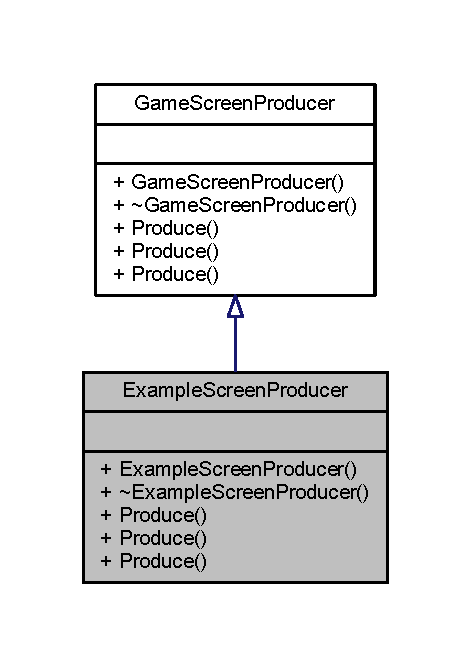
\includegraphics[width=226pt]{class_example_screen_producer__inherit__graph}
\end{center}
\end{figure}


Collaboration diagram for Example\-Screen\-Producer\-:\nopagebreak
\begin{figure}[H]
\begin{center}
\leavevmode
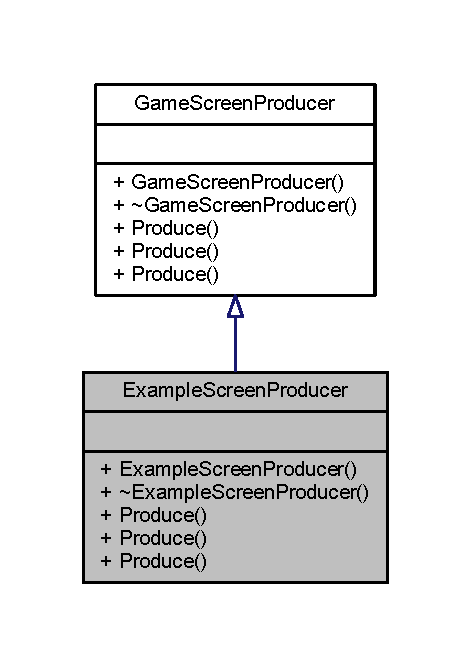
\includegraphics[width=226pt]{class_example_screen_producer__coll__graph}
\end{center}
\end{figure}
\subsection*{Public Member Functions}
\begin{DoxyCompactItemize}
\item 
\hyperlink{class_example_screen_producer_ac33eb1451e3fbd42bb112e81233dcd31}{Example\-Screen\-Producer} ()
\item 
\hyperlink{class_example_screen_producer_a1243a0aa0a1ecd2a218f9dab7b340213}{$\sim$\-Example\-Screen\-Producer} ()
\item 
\hyperlink{class_game_screen}{Game\-Screen} $\ast$ \hyperlink{class_example_screen_producer_a7eff2a8dd0085b380ba3b41fbf9d0691}{Produce} () override
\item 
\hyperlink{class_game_screen}{Game\-Screen} $\ast$ \hyperlink{class_example_screen_producer_a085da3f4766c2511f82425f66f29e07e}{Produce} (\hyperlink{class_producer_package}{Producer\-Package} Package) override
\item 
\hyperlink{class_game_screen}{Game\-Screen} $\ast$ \hyperlink{class_example_screen_producer_a3c1e2f971c209bc027201a563b0c67c8}{Produce} (\hyperlink{class_producer_package}{Producer\-Package} $\ast$Package) override
\end{DoxyCompactItemize}


\subsection{Constructor \& Destructor Documentation}
\hypertarget{class_example_screen_producer_ac33eb1451e3fbd42bb112e81233dcd31}{\index{Example\-Screen\-Producer@{Example\-Screen\-Producer}!Example\-Screen\-Producer@{Example\-Screen\-Producer}}
\index{Example\-Screen\-Producer@{Example\-Screen\-Producer}!ExampleScreenProducer@{Example\-Screen\-Producer}}
\subsubsection[{Example\-Screen\-Producer}]{\setlength{\rightskip}{0pt plus 5cm}Example\-Screen\-Producer\-::\-Example\-Screen\-Producer (
\begin{DoxyParamCaption}
{}
\end{DoxyParamCaption}
)}}\label{class_example_screen_producer_ac33eb1451e3fbd42bb112e81233dcd31}
\hypertarget{class_example_screen_producer_a1243a0aa0a1ecd2a218f9dab7b340213}{\index{Example\-Screen\-Producer@{Example\-Screen\-Producer}!$\sim$\-Example\-Screen\-Producer@{$\sim$\-Example\-Screen\-Producer}}
\index{$\sim$\-Example\-Screen\-Producer@{$\sim$\-Example\-Screen\-Producer}!ExampleScreenProducer@{Example\-Screen\-Producer}}
\subsubsection[{$\sim$\-Example\-Screen\-Producer}]{\setlength{\rightskip}{0pt plus 5cm}Example\-Screen\-Producer\-::$\sim$\-Example\-Screen\-Producer (
\begin{DoxyParamCaption}
{}
\end{DoxyParamCaption}
)}}\label{class_example_screen_producer_a1243a0aa0a1ecd2a218f9dab7b340213}


\subsection{Member Function Documentation}
\hypertarget{class_example_screen_producer_a7eff2a8dd0085b380ba3b41fbf9d0691}{\index{Example\-Screen\-Producer@{Example\-Screen\-Producer}!Produce@{Produce}}
\index{Produce@{Produce}!ExampleScreenProducer@{Example\-Screen\-Producer}}
\subsubsection[{Produce}]{\setlength{\rightskip}{0pt plus 5cm}{\bf Game\-Screen} $\ast$ Example\-Screen\-Producer\-::\-Produce (
\begin{DoxyParamCaption}
{}
\end{DoxyParamCaption}
)\hspace{0.3cm}{\ttfamily [override]}}}\label{class_example_screen_producer_a7eff2a8dd0085b380ba3b41fbf9d0691}
\hypertarget{class_example_screen_producer_a085da3f4766c2511f82425f66f29e07e}{\index{Example\-Screen\-Producer@{Example\-Screen\-Producer}!Produce@{Produce}}
\index{Produce@{Produce}!ExampleScreenProducer@{Example\-Screen\-Producer}}
\subsubsection[{Produce}]{\setlength{\rightskip}{0pt plus 5cm}{\bf Game\-Screen} $\ast$ Example\-Screen\-Producer\-::\-Produce (
\begin{DoxyParamCaption}
\item[{{\bf Producer\-Package}}]{Package}
\end{DoxyParamCaption}
)\hspace{0.3cm}{\ttfamily [override]}}}\label{class_example_screen_producer_a085da3f4766c2511f82425f66f29e07e}
\hypertarget{class_example_screen_producer_a3c1e2f971c209bc027201a563b0c67c8}{\index{Example\-Screen\-Producer@{Example\-Screen\-Producer}!Produce@{Produce}}
\index{Produce@{Produce}!ExampleScreenProducer@{Example\-Screen\-Producer}}
\subsubsection[{Produce}]{\setlength{\rightskip}{0pt plus 5cm}{\bf Game\-Screen} $\ast$ Example\-Screen\-Producer\-::\-Produce (
\begin{DoxyParamCaption}
\item[{{\bf Producer\-Package} $\ast$}]{Package}
\end{DoxyParamCaption}
)\hspace{0.3cm}{\ttfamily [override]}}}\label{class_example_screen_producer_a3c1e2f971c209bc027201a563b0c67c8}


The documentation for this class was generated from the following files\-:\begin{DoxyCompactItemize}
\item 
D\-:/\-Users/tom/\-Documents/\-Visual Studio 2013/\-Projects/\-Revelatorframework/\-Revelatorframework/\hyperlink{_example_screen_producer_8hpp}{Example\-Screen\-Producer.\-hpp}\item 
D\-:/\-Users/tom/\-Documents/\-Visual Studio 2013/\-Projects/\-Revelatorframework/\-Revelatorframework/\hyperlink{_example_screen_producer_8cpp}{Example\-Screen\-Producer.\-cpp}\end{DoxyCompactItemize}

\hypertarget{class_example_test_screen}{\section{Example\-Test\-Screen Class Reference}
\label{class_example_test_screen}\index{Example\-Test\-Screen@{Example\-Test\-Screen}}
}


{\ttfamily \#include $<$Example\-Test\-Screen.\-hpp$>$}



Inheritance diagram for Example\-Test\-Screen\-:\nopagebreak
\begin{figure}[H]
\begin{center}
\leavevmode
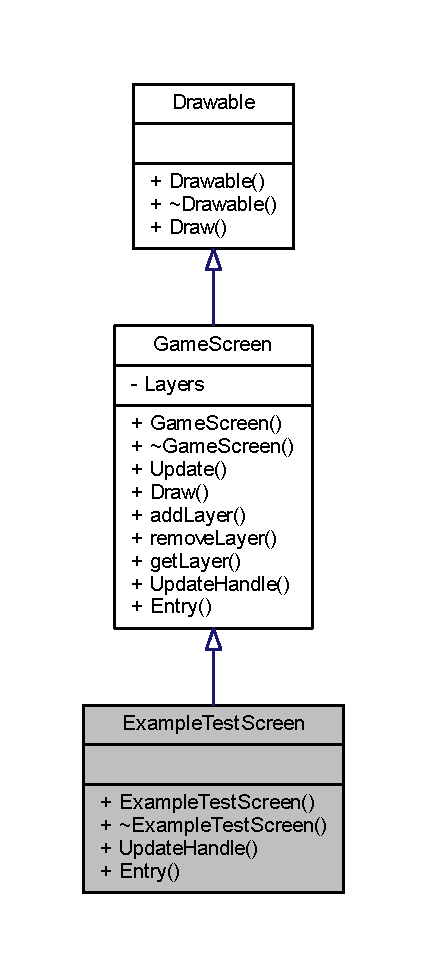
\includegraphics[width=205pt]{class_example_test_screen__inherit__graph}
\end{center}
\end{figure}


Collaboration diagram for Example\-Test\-Screen\-:\nopagebreak
\begin{figure}[H]
\begin{center}
\leavevmode
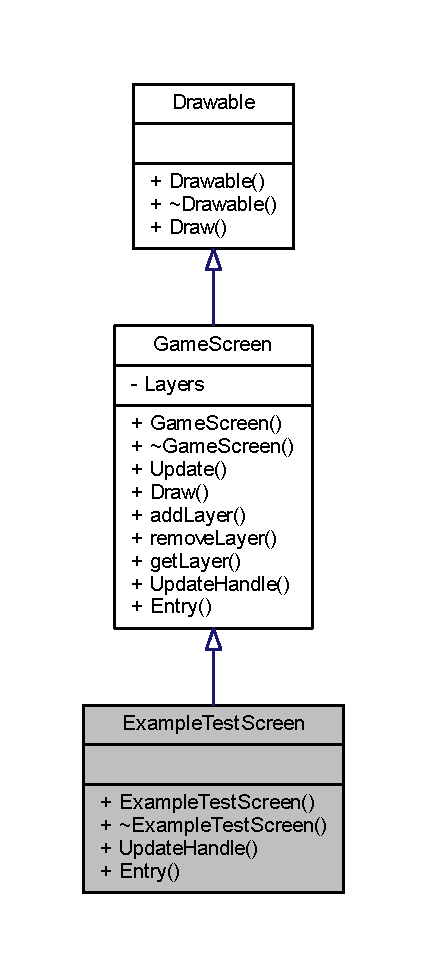
\includegraphics[width=205pt]{class_example_test_screen__coll__graph}
\end{center}
\end{figure}
\subsection*{Public Member Functions}
\begin{DoxyCompactItemize}
\item 
\hyperlink{class_example_test_screen_aa98a7d000384c1352178d179414c1435}{Example\-Test\-Screen} ()
\item 
\hyperlink{class_example_test_screen_a1b9bc6ee5fa89ce2460b2d60ee9ec924}{$\sim$\-Example\-Test\-Screen} ()
\item 
void \hyperlink{class_example_test_screen_a44f0c5ae87832e341d6eb9b44f811969}{Update\-Handle} (const \hyperlink{class_update_data}{Update\-Data} \&updateobject) override
\item 
void \hyperlink{class_example_test_screen_ac125607c70fd06f1a56c97f4f93cdd8b}{Entry} (\hyperlink{class_entry_object}{Entry\-Object} object) override
\end{DoxyCompactItemize}


\subsection{Constructor \& Destructor Documentation}
\hypertarget{class_example_test_screen_aa98a7d000384c1352178d179414c1435}{\index{Example\-Test\-Screen@{Example\-Test\-Screen}!Example\-Test\-Screen@{Example\-Test\-Screen}}
\index{Example\-Test\-Screen@{Example\-Test\-Screen}!ExampleTestScreen@{Example\-Test\-Screen}}
\subsubsection[{Example\-Test\-Screen}]{\setlength{\rightskip}{0pt plus 5cm}Example\-Test\-Screen\-::\-Example\-Test\-Screen (
\begin{DoxyParamCaption}
{}
\end{DoxyParamCaption}
)}}\label{class_example_test_screen_aa98a7d000384c1352178d179414c1435}
\hypertarget{class_example_test_screen_a1b9bc6ee5fa89ce2460b2d60ee9ec924}{\index{Example\-Test\-Screen@{Example\-Test\-Screen}!$\sim$\-Example\-Test\-Screen@{$\sim$\-Example\-Test\-Screen}}
\index{$\sim$\-Example\-Test\-Screen@{$\sim$\-Example\-Test\-Screen}!ExampleTestScreen@{Example\-Test\-Screen}}
\subsubsection[{$\sim$\-Example\-Test\-Screen}]{\setlength{\rightskip}{0pt plus 5cm}Example\-Test\-Screen\-::$\sim$\-Example\-Test\-Screen (
\begin{DoxyParamCaption}
{}
\end{DoxyParamCaption}
)}}\label{class_example_test_screen_a1b9bc6ee5fa89ce2460b2d60ee9ec924}


\subsection{Member Function Documentation}
\hypertarget{class_example_test_screen_ac125607c70fd06f1a56c97f4f93cdd8b}{\index{Example\-Test\-Screen@{Example\-Test\-Screen}!Entry@{Entry}}
\index{Entry@{Entry}!ExampleTestScreen@{Example\-Test\-Screen}}
\subsubsection[{Entry}]{\setlength{\rightskip}{0pt plus 5cm}void Example\-Test\-Screen\-::\-Entry (
\begin{DoxyParamCaption}
\item[{{\bf Entry\-Object}}]{object}
\end{DoxyParamCaption}
)\hspace{0.3cm}{\ttfamily [inline]}, {\ttfamily [override]}, {\ttfamily [virtual]}}}\label{class_example_test_screen_ac125607c70fd06f1a56c97f4f93cdd8b}


Implements \hyperlink{class_game_screen_a76e44a105b36f32b68a0ba7a325971b0}{Game\-Screen}.

\hypertarget{class_example_test_screen_a44f0c5ae87832e341d6eb9b44f811969}{\index{Example\-Test\-Screen@{Example\-Test\-Screen}!Update\-Handle@{Update\-Handle}}
\index{Update\-Handle@{Update\-Handle}!ExampleTestScreen@{Example\-Test\-Screen}}
\subsubsection[{Update\-Handle}]{\setlength{\rightskip}{0pt plus 5cm}void Example\-Test\-Screen\-::\-Update\-Handle (
\begin{DoxyParamCaption}
\item[{const {\bf Update\-Data} \&}]{updateobject}
\end{DoxyParamCaption}
)\hspace{0.3cm}{\ttfamily [inline]}, {\ttfamily [override]}, {\ttfamily [virtual]}}}\label{class_example_test_screen_a44f0c5ae87832e341d6eb9b44f811969}


Implements \hyperlink{class_game_screen_a5ffce37600960d6c8885bf071461998c}{Game\-Screen}.



The documentation for this class was generated from the following files\-:\begin{DoxyCompactItemize}
\item 
D\-:/\-Users/tom/\-Documents/\-Visual Studio 2013/\-Projects/\-Revelatorframework/\-Revelatorframework/\hyperlink{_example_test_screen_8hpp}{Example\-Test\-Screen.\-hpp}\item 
D\-:/\-Users/tom/\-Documents/\-Visual Studio 2013/\-Projects/\-Revelatorframework/\-Revelatorframework/\hyperlink{_example_test_screen_8cpp}{Example\-Test\-Screen.\-cpp}\end{DoxyCompactItemize}

\hypertarget{class_game_component}{\section{Game\-Component Class Reference}
\label{class_game_component}\index{Game\-Component@{Game\-Component}}
}


Inheritance diagram for Game\-Component\-:\nopagebreak
\begin{figure}[H]
\begin{center}
\leavevmode
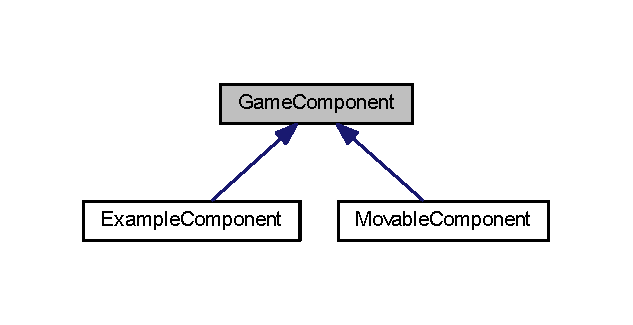
\includegraphics[width=304pt]{class_game_component__inherit__graph}
\end{center}
\end{figure}


Collaboration diagram for Game\-Component\-:\nopagebreak
\begin{figure}[H]
\begin{center}
\leavevmode
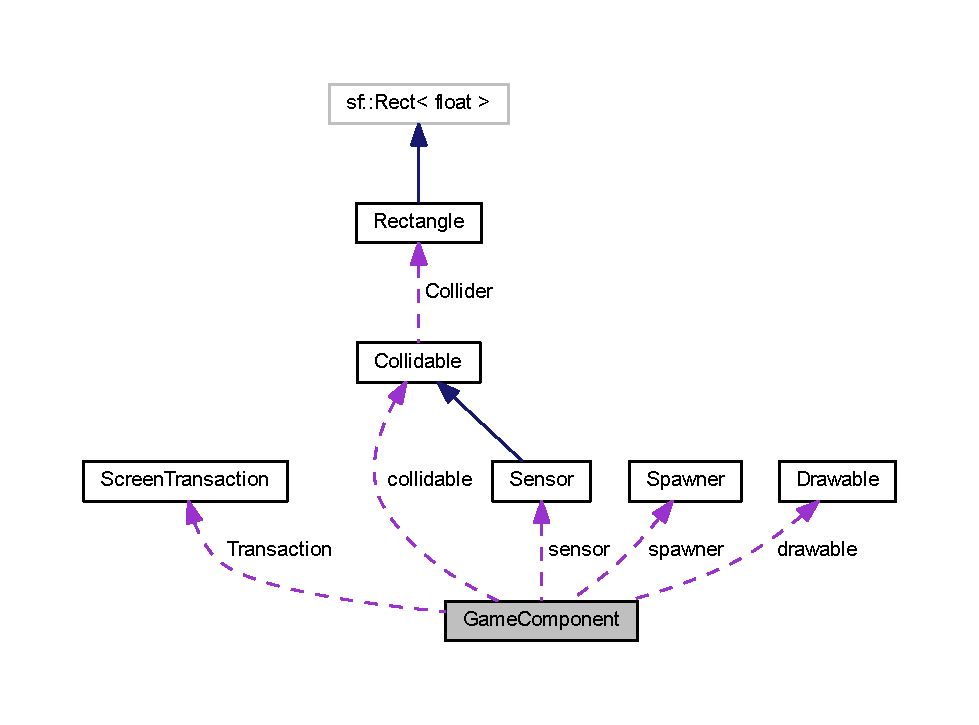
\includegraphics[width=350pt]{class_game_component__coll__graph}
\end{center}
\end{figure}
\subsection*{Public Member Functions}
\begin{DoxyCompactItemize}
\item 
\hypertarget{class_game_component_ac1eefc88d46d10f869939a7bab5a498b}{{\bfseries Game\-Component} (float x, float y)}\label{class_game_component_ac1eefc88d46d10f869939a7bab5a498b}

\item 
\hypertarget{class_game_component_a3338305ddce8cb75296ba23e1c29cf0f}{{\bfseries Game\-Component} (sf\-::\-Vector2f Pos)}\label{class_game_component_a3338305ddce8cb75296ba23e1c29cf0f}

\item 
\hypertarget{class_game_component_a01b3434d7bf6a63552e7ea4fd68744fe}{virtual void {\bfseries Update} (\hyperlink{class_update_data}{Update\-Data} $\ast$updateobject)=0}\label{class_game_component_a01b3434d7bf6a63552e7ea4fd68744fe}

\item 
\hypertarget{class_game_component_a333932780a30df552333d02669c593bc}{virtual void {\bfseries Collide} (\hyperlink{class_game_component}{Game\-Component} $\ast$colider)=0}\label{class_game_component_a333932780a30df552333d02669c593bc}

\item 
\hypertarget{class_game_component_a63c3e40531340490712b789d0d821743}{virtual void {\bfseries Draw} (sf\-::\-Render\-Window \&window, sf\-::\-Vector2f offset)=0}\label{class_game_component_a63c3e40531340490712b789d0d821743}

\item 
\hypertarget{class_game_component_a5dc0e3d5d8aa6be47d4392dc0ebe566d}{virtual bool {\bfseries has\-Transaction} ()}\label{class_game_component_a5dc0e3d5d8aa6be47d4392dc0ebe566d}

\item 
\hypertarget{class_game_component_a5473b7d5e5c1e6f6c94e1d665cb4623c}{virtual void {\bfseries set\-Transaction} (\hyperlink{class_screen_transaction}{Screen\-Transaction} $\ast$transaction)}\label{class_game_component_a5473b7d5e5c1e6f6c94e1d665cb4623c}

\item 
\hypertarget{class_game_component_a84b6f548c5045a179b9d2c33c3944f10}{virtual \hyperlink{class_screen_transaction}{Screen\-Transaction} $\ast$ {\bfseries get\-Transaction} ()}\label{class_game_component_a84b6f548c5045a179b9d2c33c3944f10}

\item 
\hypertarget{class_game_component_aabb5e9e8ed6aa3a82f5d5b5733bf201c}{sf\-::\-Vector2f $\ast$ {\bfseries get\-Position} ()}\label{class_game_component_aabb5e9e8ed6aa3a82f5d5b5733bf201c}

\item 
\hypertarget{class_game_component_ae1218b48879f706b5686bcedd4c51022}{void {\bfseries set\-Position} (sf\-::\-Vector2f $\ast$pos)}\label{class_game_component_ae1218b48879f706b5686bcedd4c51022}

\item 
\hypertarget{class_game_component_ae5a83de3b78cc5ce0f43316dd45de20d}{bool {\bfseries has\-Drawable} ()}\label{class_game_component_ae5a83de3b78cc5ce0f43316dd45de20d}

\item 
\hypertarget{class_game_component_a8595ee50d296557bcf1af3ba5283c311}{bool {\bfseries has\-Collidable} ()}\label{class_game_component_a8595ee50d296557bcf1af3ba5283c311}

\item 
\hypertarget{class_game_component_af61ba1bd218ff2aca92443c89375c222}{bool {\bfseries has\-Sensor} ()}\label{class_game_component_af61ba1bd218ff2aca92443c89375c222}

\item 
\hypertarget{class_game_component_ae6e938bb93586ad8820316368065c174}{bool {\bfseries has\-Spawner} ()}\label{class_game_component_ae6e938bb93586ad8820316368065c174}

\item 
\hypertarget{class_game_component_a6b5db3e878b861296d6cc3a0f4ee6528}{\hyperlink{class_drawable}{Drawable} $\ast$ {\bfseries get\-Drawable} ()}\label{class_game_component_a6b5db3e878b861296d6cc3a0f4ee6528}

\item 
\hypertarget{class_game_component_a09eae8038373202d058179080643f75b}{\hyperlink{class_collidable}{Collidable} $\ast$ {\bfseries get\-Collidable} ()}\label{class_game_component_a09eae8038373202d058179080643f75b}

\item 
\hypertarget{class_game_component_afca864b925be82f9c54711c75dc7be12}{\hyperlink{class_sensor}{Sensor} $\ast$ {\bfseries get\-Sensor} ()}\label{class_game_component_afca864b925be82f9c54711c75dc7be12}

\item 
\hypertarget{class_game_component_ab6db9e2e5f501ca360b08a7fc6a19644}{\hyperlink{class_spawner}{Spawner} $\ast$ {\bfseries get\-Spawner} ()}\label{class_game_component_ab6db9e2e5f501ca360b08a7fc6a19644}

\end{DoxyCompactItemize}
\subsection*{Protected Attributes}
\begin{DoxyCompactItemize}
\item 
\hypertarget{class_game_component_ab1037207fec65ac5fe65dec1e22f0566}{std\-::string {\bfseries Name}}\label{class_game_component_ab1037207fec65ac5fe65dec1e22f0566}

\item 
\hypertarget{class_game_component_ac8d794e78280785eb956eaff044f74b2}{int {\bfseries I\-D}}\label{class_game_component_ac8d794e78280785eb956eaff044f74b2}

\item 
\hypertarget{class_game_component_ae8c59f47f6723d108eb481a160607e98}{\hyperlink{class_screen_transaction}{Screen\-Transaction} $\ast$ {\bfseries Transaction}}\label{class_game_component_ae8c59f47f6723d108eb481a160607e98}

\item 
\hypertarget{class_game_component_acc3109bb4ae36112eb8796e067160c59}{sf\-::\-Vector2f $\ast$ {\bfseries Position}}\label{class_game_component_acc3109bb4ae36112eb8796e067160c59}

\item 
\hypertarget{class_game_component_acb73190345f4933825e9c8b8d5030438}{\hyperlink{class_drawable}{Drawable} $\ast$ {\bfseries drawable}}\label{class_game_component_acb73190345f4933825e9c8b8d5030438}

\item 
\hypertarget{class_game_component_aa91bd3600bd5964b55c7806dcfd1c862}{\hyperlink{class_collidable}{Collidable} $\ast$ {\bfseries collidable}}\label{class_game_component_aa91bd3600bd5964b55c7806dcfd1c862}

\item 
\hypertarget{class_game_component_ad585bf57df228afc83fbf777142e51bd}{\hyperlink{class_sensor}{Sensor} $\ast$ {\bfseries sensor}}\label{class_game_component_ad585bf57df228afc83fbf777142e51bd}

\item 
\hypertarget{class_game_component_a15caaab21ec2e8eb9d438a25afbef4da}{\hyperlink{class_spawner}{Spawner} $\ast$ {\bfseries spawner}}\label{class_game_component_a15caaab21ec2e8eb9d438a25afbef4da}

\end{DoxyCompactItemize}


The documentation for this class was generated from the following files\-:\begin{DoxyCompactItemize}
\item 
Revelatorfromework/Game\-Component.\-hpp\item 
Revelatorfromework/Game\-Component.\-cpp\end{DoxyCompactItemize}

\hypertarget{class_game_factory}{\section{Game\-Factory Class Reference}
\label{class_game_factory}\index{Game\-Factory@{Game\-Factory}}
}


{\ttfamily \#include $<$Game\-Factory.\-hpp$>$}



Collaboration diagram for Game\-Factory\-:\nopagebreak
\begin{figure}[H]
\begin{center}
\leavevmode
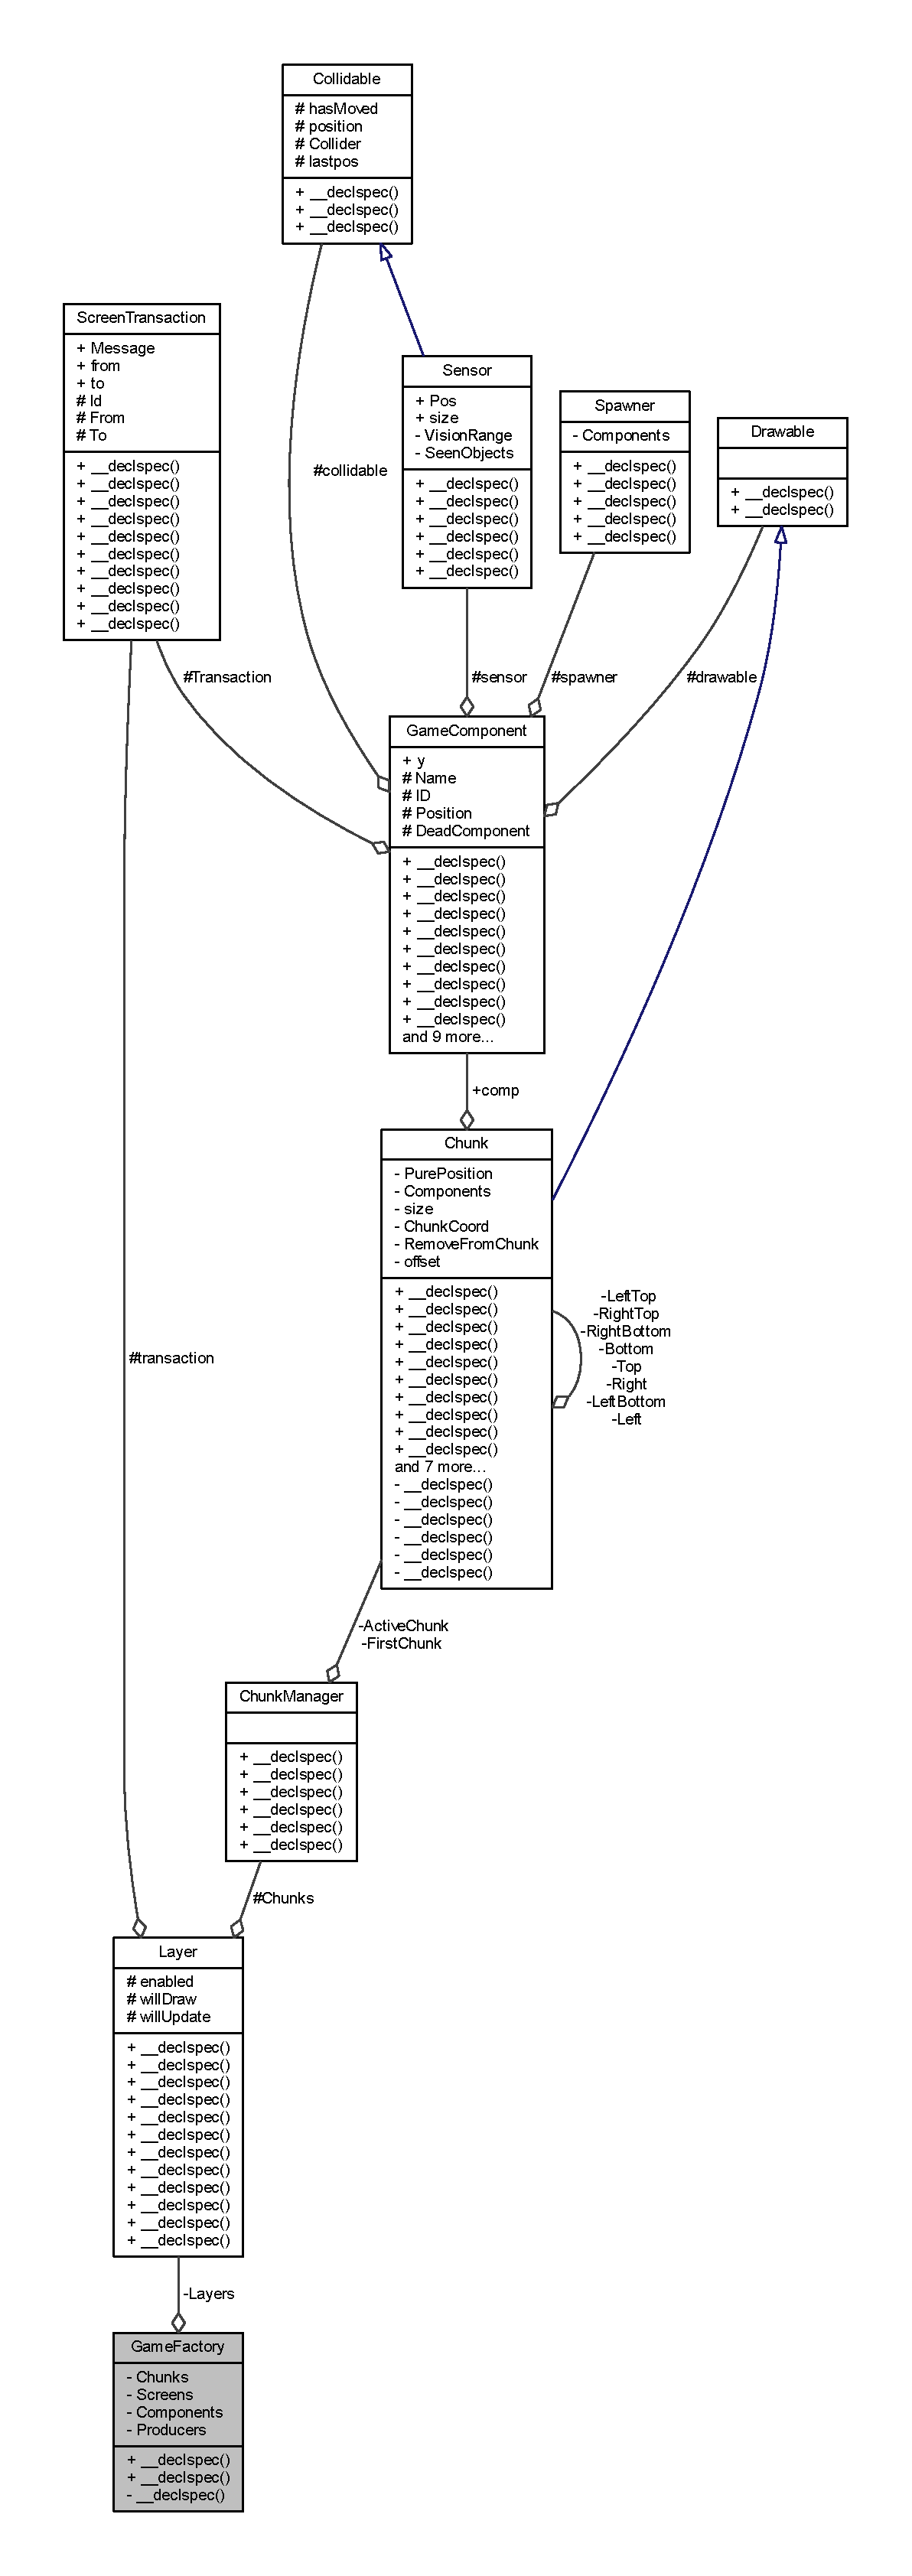
\includegraphics[width=217pt]{class_game_factory__coll__graph}
\end{center}
\end{figure}
\subsection*{Public Member Functions}
\begin{DoxyCompactItemize}
\item 
\hyperlink{class_game_factory_a0cbbb4c198cab19386d67bfe7891b785}{$\sim$\-Game\-Factory} ()
\item 
\hyperlink{class_game_screen}{Game\-Screen} $\ast$ \hyperlink{class_game_factory_ad293f5a8811d9106753916cef819fbce}{Produce\-Screen} (std\-::string screenname)
\item 
void \hyperlink{class_game_factory_a77df8b5e97869b7d7b667c0852191e20}{Register\-Object\-Producer} (std\-::string Name, \hyperlink{class_game_object_producer}{Game\-Object\-Producer} $\ast$producer)
\item 
void \hyperlink{class_game_factory_a3a20ae04c8ff992ad080b9742f5831c0}{Register\-Layer\-Producer} (std\-::string Name, \hyperlink{class_layer_producer}{Layer\-Producer} $\ast$producer)
\item 
void \hyperlink{class_game_factory_ad3c85f8654dd2c3aeb7a2b17df05cceb}{Register\-Screen\-Producer} (std\-::string Name, \hyperlink{class_game_screen_producer}{Game\-Screen\-Producer} $\ast$producer)
\item 
\hyperlink{class_game_component}{Game\-Component} $\ast$ \hyperlink{class_game_factory_a521cf5410b97240789a9cc54404d6a2f}{Produce\-Game\-Object} (std\-::string Name)
\item 
\hyperlink{class_game_component}{Game\-Component} $\ast$ \hyperlink{class_game_factory_a0ed92342411d80d6080294c29ac2c54e}{Produce\-Game\-Object} (std\-::string Name, \hyperlink{class_producer_package}{Producer\-Package} package)
\item 
void \hyperlink{class_game_factory_a7a130a6b0bff752fdd8223616a5f046f}{Delete\-Decommisioned} ()
\item 
\hyperlink{class_game_factory_a694a26c694da014dc5ced9d85a2aaaa1}{Game\-Factory} (const \hyperlink{class_game_factory}{Game\-Factory} \&utils)=delete
\item 
\hyperlink{class_game_factory}{Game\-Factory} \& \hyperlink{class_game_factory_ac9e48fb53d87829930bbc447133d9c25}{operator=} (const \hyperlink{class_game_factory}{Game\-Factory} \&utils)=delete
\end{DoxyCompactItemize}
\subsection*{Static Public Member Functions}
\begin{DoxyCompactItemize}
\item 
static \hyperlink{class_game_factory}{Game\-Factory} \& \hyperlink{class_game_factory_a0b1eef0e66b8f6ff8277f6d5fb4b8e0d}{get\-Instance} ()
\end{DoxyCompactItemize}
\subsection*{Private Member Functions}
\begin{DoxyCompactItemize}
\item 
\hyperlink{class_game_factory_a37c039131801be05d138bd76bb125ab3}{Game\-Factory} ()
\item 
\hyperlink{class_layer}{Layer} $\ast$ \hyperlink{class_game_factory_a0c24ad925bf672c6fb721dfaaf993f9d}{Produce\-Layer} (std\-::string layername, int Chunk\-Size, const int \hyperlink{class_game_factory_a77496a7ea1e2fa54acb18c499b3bd3bb}{Chunks}, bool enabled, bool willupdate, bool willdraw, \hyperlink{class_producer_package}{Producer\-Package} package, std\-::string layertype)
\end{DoxyCompactItemize}
\subsection*{Private Attributes}
\begin{DoxyCompactItemize}
\item 
std\-::list$<$ \hyperlink{class_layer}{Layer} $\ast$ $>$ \hyperlink{class_game_factory_a7ab6a968cb7af49813407fe66927c126}{Layers}
\item 
std\-::list$<$ \hyperlink{class_chunk}{Chunk} $\ast$ $>$ \hyperlink{class_game_factory_a77496a7ea1e2fa54acb18c499b3bd3bb}{Chunks}
\item 
std\-::list$<$ \hyperlink{class_game_screen}{Game\-Screen} $\ast$ $>$ \hyperlink{class_game_factory_a16a8135f6d6b1b60c0d08b39340b34cc}{Screens}
\item 
std\-::list$<$ \hyperlink{class_game_component}{Game\-Component} $\ast$ $>$ \hyperlink{class_game_factory_a90fc6360610babaf3d2d880f782772b3}{Components}
\item 
std\-::map$<$ std\-::string, \\*
\hyperlink{class_game_object_producer}{Game\-Object\-Producer} $\ast$ $>$ \hyperlink{class_game_factory_ab72819fc3f241243d44827f75e0a2886}{Object\-Producers}
\item 
std\-::map$<$ std\-::string, \\*
\hyperlink{class_game_screen_producer}{Game\-Screen\-Producer} $\ast$ $>$ \hyperlink{class_game_factory_aa65ba67e6c3fc56ec228c801e02352c8}{Screen\-Producers}
\item 
std\-::map$<$ std\-::string, \\*
\hyperlink{class_layer_producer}{Layer\-Producer} $\ast$ $>$ \hyperlink{class_game_factory_adfadca1996a3982f4b45c67ced1520f2}{Layer\-Producers}
\end{DoxyCompactItemize}


\subsection{Constructor \& Destructor Documentation}
\hypertarget{class_game_factory_a0cbbb4c198cab19386d67bfe7891b785}{\index{Game\-Factory@{Game\-Factory}!$\sim$\-Game\-Factory@{$\sim$\-Game\-Factory}}
\index{$\sim$\-Game\-Factory@{$\sim$\-Game\-Factory}!GameFactory@{Game\-Factory}}
\subsubsection[{$\sim$\-Game\-Factory}]{\setlength{\rightskip}{0pt plus 5cm}Game\-Factory\-::$\sim$\-Game\-Factory (
\begin{DoxyParamCaption}
{}
\end{DoxyParamCaption}
)}}\label{class_game_factory_a0cbbb4c198cab19386d67bfe7891b785}
\hypertarget{class_game_factory_a694a26c694da014dc5ced9d85a2aaaa1}{\index{Game\-Factory@{Game\-Factory}!Game\-Factory@{Game\-Factory}}
\index{Game\-Factory@{Game\-Factory}!GameFactory@{Game\-Factory}}
\subsubsection[{Game\-Factory}]{\setlength{\rightskip}{0pt plus 5cm}Game\-Factory\-::\-Game\-Factory (
\begin{DoxyParamCaption}
\item[{const {\bf Game\-Factory} \&}]{utils}
\end{DoxyParamCaption}
)\hspace{0.3cm}{\ttfamily [delete]}}}\label{class_game_factory_a694a26c694da014dc5ced9d85a2aaaa1}
\hypertarget{class_game_factory_a37c039131801be05d138bd76bb125ab3}{\index{Game\-Factory@{Game\-Factory}!Game\-Factory@{Game\-Factory}}
\index{Game\-Factory@{Game\-Factory}!GameFactory@{Game\-Factory}}
\subsubsection[{Game\-Factory}]{\setlength{\rightskip}{0pt plus 5cm}Game\-Factory\-::\-Game\-Factory (
\begin{DoxyParamCaption}
{}
\end{DoxyParamCaption}
)\hspace{0.3cm}{\ttfamily [private]}}}\label{class_game_factory_a37c039131801be05d138bd76bb125ab3}


\subsection{Member Function Documentation}
\hypertarget{class_game_factory_a7a130a6b0bff752fdd8223616a5f046f}{\index{Game\-Factory@{Game\-Factory}!Delete\-Decommisioned@{Delete\-Decommisioned}}
\index{Delete\-Decommisioned@{Delete\-Decommisioned}!GameFactory@{Game\-Factory}}
\subsubsection[{Delete\-Decommisioned}]{\setlength{\rightskip}{0pt plus 5cm}void Game\-Factory\-::\-Delete\-Decommisioned (
\begin{DoxyParamCaption}
{}
\end{DoxyParamCaption}
)}}\label{class_game_factory_a7a130a6b0bff752fdd8223616a5f046f}


Here is the caller graph for this function\-:\nopagebreak
\begin{figure}[H]
\begin{center}
\leavevmode
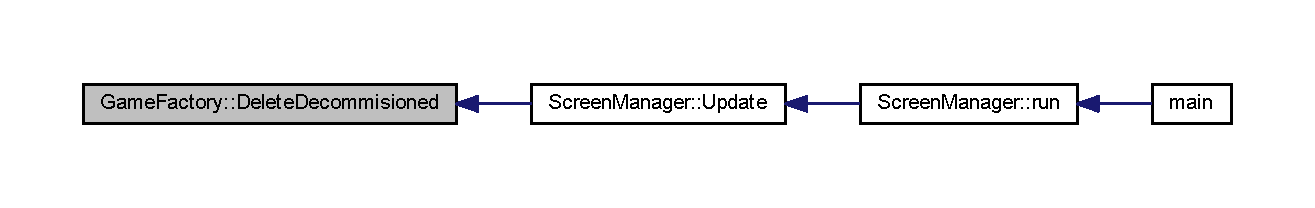
\includegraphics[width=350pt]{class_game_factory_a7a130a6b0bff752fdd8223616a5f046f_icgraph}
\end{center}
\end{figure}


\hypertarget{class_game_factory_a0b1eef0e66b8f6ff8277f6d5fb4b8e0d}{\index{Game\-Factory@{Game\-Factory}!get\-Instance@{get\-Instance}}
\index{get\-Instance@{get\-Instance}!GameFactory@{Game\-Factory}}
\subsubsection[{get\-Instance}]{\setlength{\rightskip}{0pt plus 5cm}{\bf Game\-Factory} \& Game\-Factory\-::get\-Instance (
\begin{DoxyParamCaption}
{}
\end{DoxyParamCaption}
)\hspace{0.3cm}{\ttfamily [static]}}}\label{class_game_factory_a0b1eef0e66b8f6ff8277f6d5fb4b8e0d}


Here is the caller graph for this function\-:\nopagebreak
\begin{figure}[H]
\begin{center}
\leavevmode
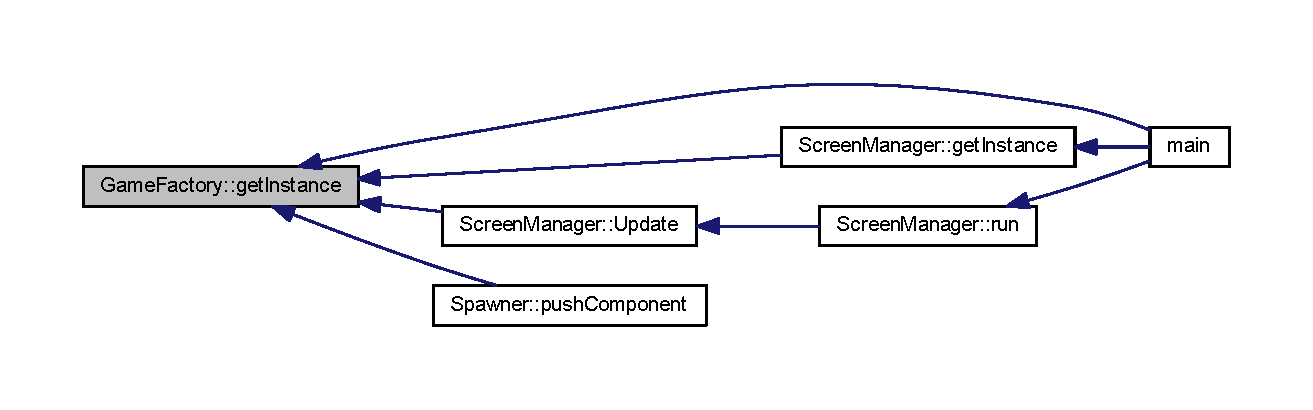
\includegraphics[width=350pt]{class_game_factory_a0b1eef0e66b8f6ff8277f6d5fb4b8e0d_icgraph}
\end{center}
\end{figure}


\hypertarget{class_game_factory_ac9e48fb53d87829930bbc447133d9c25}{\index{Game\-Factory@{Game\-Factory}!operator=@{operator=}}
\index{operator=@{operator=}!GameFactory@{Game\-Factory}}
\subsubsection[{operator=}]{\setlength{\rightskip}{0pt plus 5cm}{\bf Game\-Factory}\& Game\-Factory\-::operator= (
\begin{DoxyParamCaption}
\item[{const {\bf Game\-Factory} \&}]{utils}
\end{DoxyParamCaption}
)\hspace{0.3cm}{\ttfamily [delete]}}}\label{class_game_factory_ac9e48fb53d87829930bbc447133d9c25}
\hypertarget{class_game_factory_a521cf5410b97240789a9cc54404d6a2f}{\index{Game\-Factory@{Game\-Factory}!Produce\-Game\-Object@{Produce\-Game\-Object}}
\index{Produce\-Game\-Object@{Produce\-Game\-Object}!GameFactory@{Game\-Factory}}
\subsubsection[{Produce\-Game\-Object}]{\setlength{\rightskip}{0pt plus 5cm}{\bf Game\-Component} $\ast$ Game\-Factory\-::\-Produce\-Game\-Object (
\begin{DoxyParamCaption}
\item[{std\-::string}]{Name}
\end{DoxyParamCaption}
)}}\label{class_game_factory_a521cf5410b97240789a9cc54404d6a2f}


Here is the caller graph for this function\-:\nopagebreak
\begin{figure}[H]
\begin{center}
\leavevmode
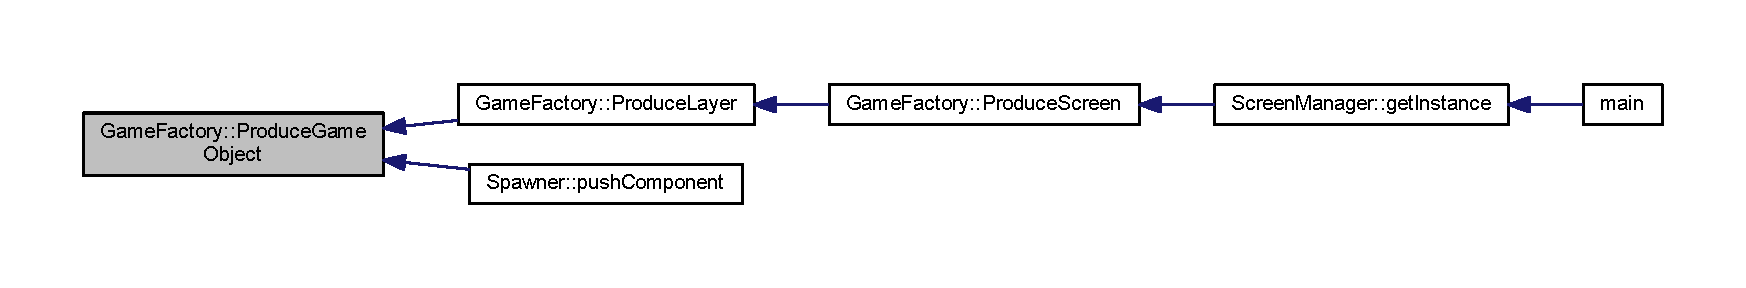
\includegraphics[width=350pt]{class_game_factory_a521cf5410b97240789a9cc54404d6a2f_icgraph}
\end{center}
\end{figure}


\hypertarget{class_game_factory_a0ed92342411d80d6080294c29ac2c54e}{\index{Game\-Factory@{Game\-Factory}!Produce\-Game\-Object@{Produce\-Game\-Object}}
\index{Produce\-Game\-Object@{Produce\-Game\-Object}!GameFactory@{Game\-Factory}}
\subsubsection[{Produce\-Game\-Object}]{\setlength{\rightskip}{0pt plus 5cm}{\bf Game\-Component} $\ast$ Game\-Factory\-::\-Produce\-Game\-Object (
\begin{DoxyParamCaption}
\item[{std\-::string}]{Name, }
\item[{{\bf Producer\-Package}}]{package}
\end{DoxyParamCaption}
)}}\label{class_game_factory_a0ed92342411d80d6080294c29ac2c54e}
\hypertarget{class_game_factory_a0c24ad925bf672c6fb721dfaaf993f9d}{\index{Game\-Factory@{Game\-Factory}!Produce\-Layer@{Produce\-Layer}}
\index{Produce\-Layer@{Produce\-Layer}!GameFactory@{Game\-Factory}}
\subsubsection[{Produce\-Layer}]{\setlength{\rightskip}{0pt plus 5cm}{\bf Layer} $\ast$ Game\-Factory\-::\-Produce\-Layer (
\begin{DoxyParamCaption}
\item[{std\-::string}]{layername, }
\item[{int}]{Chunk\-Size, }
\item[{const int}]{Chunks, }
\item[{bool}]{enabled, }
\item[{bool}]{willupdate, }
\item[{bool}]{willdraw, }
\item[{{\bf Producer\-Package}}]{package, }
\item[{std\-::string}]{layertype}
\end{DoxyParamCaption}
)\hspace{0.3cm}{\ttfamily [private]}}}\label{class_game_factory_a0c24ad925bf672c6fb721dfaaf993f9d}


Here is the call graph for this function\-:\nopagebreak
\begin{figure}[H]
\begin{center}
\leavevmode
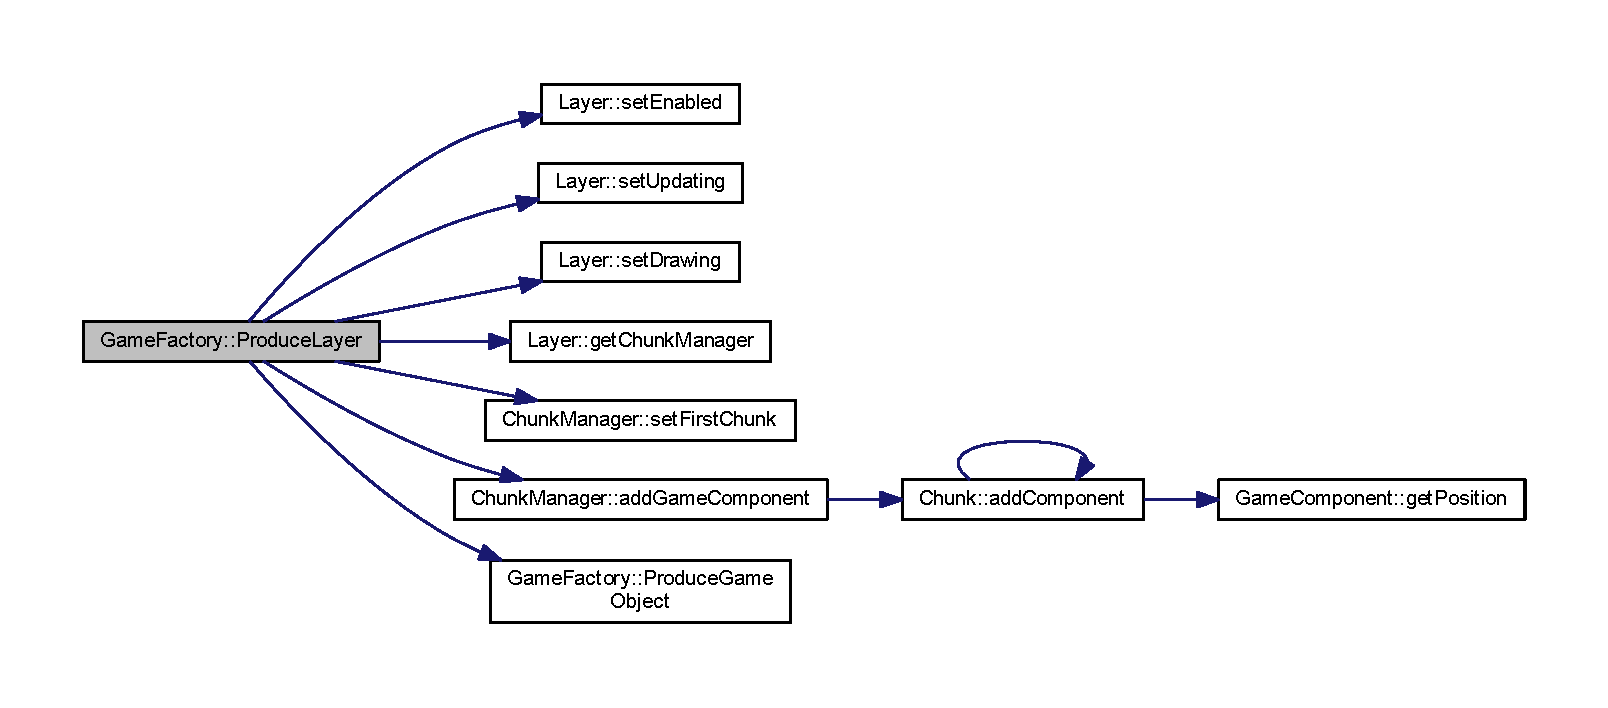
\includegraphics[width=350pt]{class_game_factory_a0c24ad925bf672c6fb721dfaaf993f9d_cgraph}
\end{center}
\end{figure}




Here is the caller graph for this function\-:\nopagebreak
\begin{figure}[H]
\begin{center}
\leavevmode
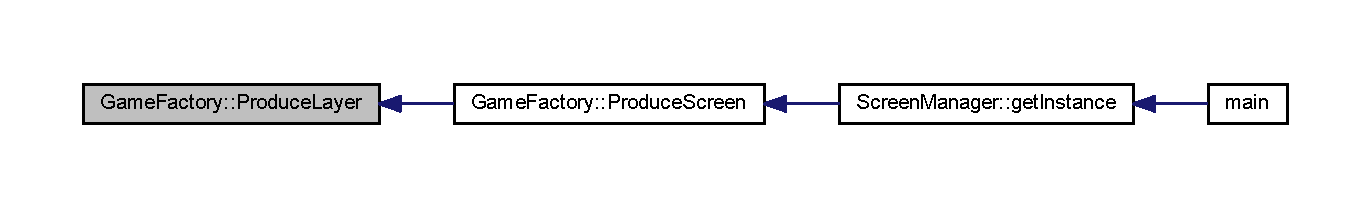
\includegraphics[width=350pt]{class_game_factory_a0c24ad925bf672c6fb721dfaaf993f9d_icgraph}
\end{center}
\end{figure}


\hypertarget{class_game_factory_ad293f5a8811d9106753916cef819fbce}{\index{Game\-Factory@{Game\-Factory}!Produce\-Screen@{Produce\-Screen}}
\index{Produce\-Screen@{Produce\-Screen}!GameFactory@{Game\-Factory}}
\subsubsection[{Produce\-Screen}]{\setlength{\rightskip}{0pt plus 5cm}{\bf Game\-Screen} $\ast$ Game\-Factory\-::\-Produce\-Screen (
\begin{DoxyParamCaption}
\item[{std\-::string}]{screenname}
\end{DoxyParamCaption}
)}}\label{class_game_factory_ad293f5a8811d9106753916cef819fbce}


Here is the call graph for this function\-:\nopagebreak
\begin{figure}[H]
\begin{center}
\leavevmode
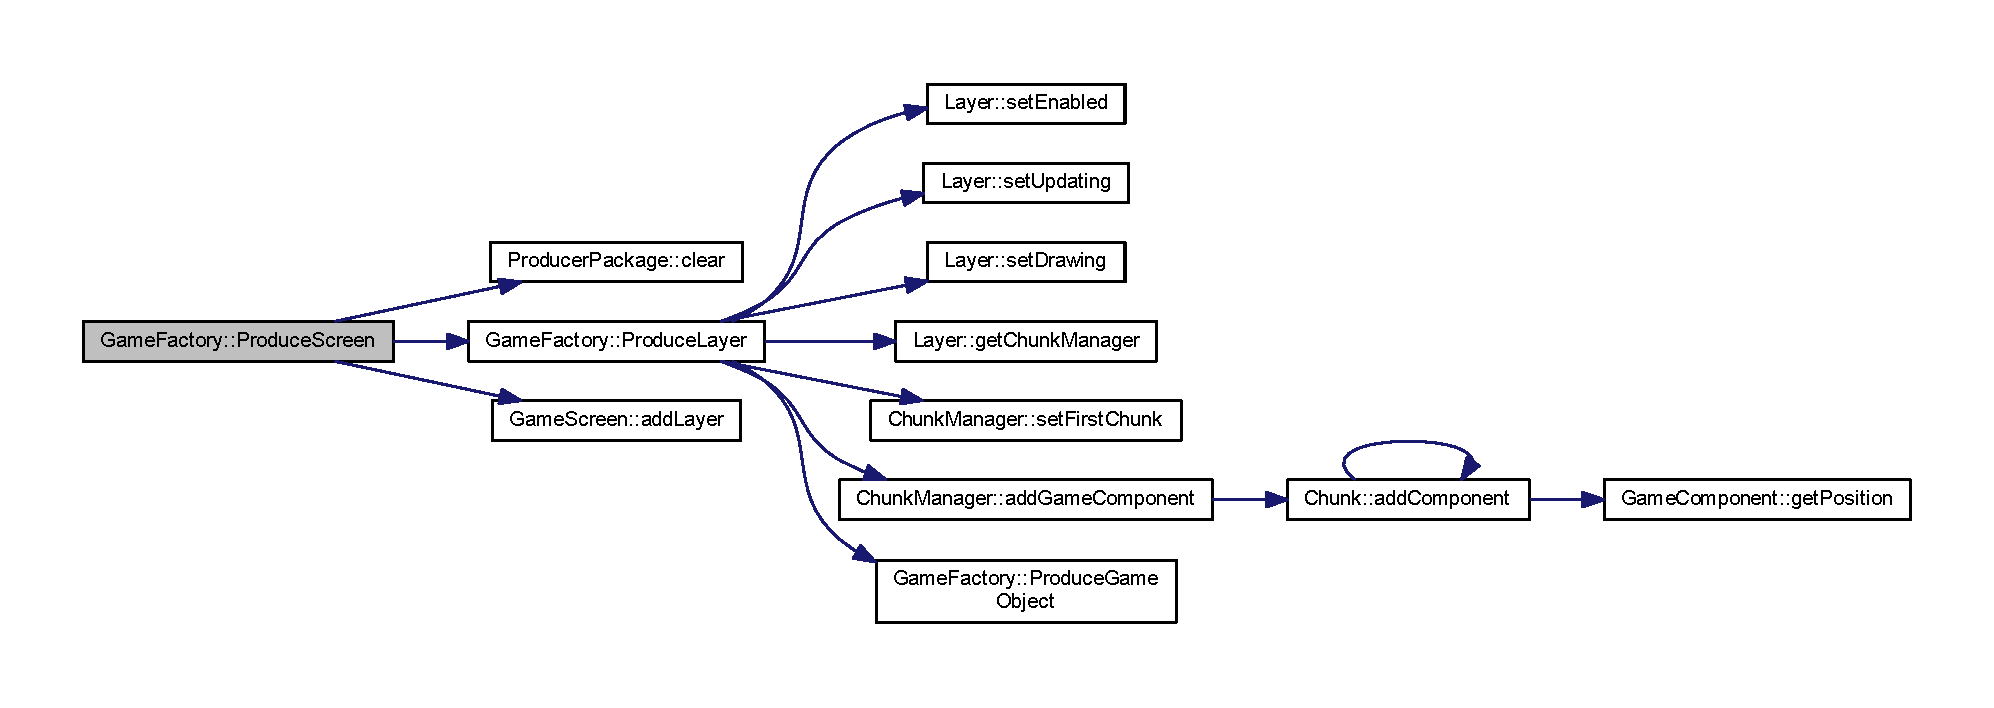
\includegraphics[width=350pt]{class_game_factory_ad293f5a8811d9106753916cef819fbce_cgraph}
\end{center}
\end{figure}




Here is the caller graph for this function\-:\nopagebreak
\begin{figure}[H]
\begin{center}
\leavevmode
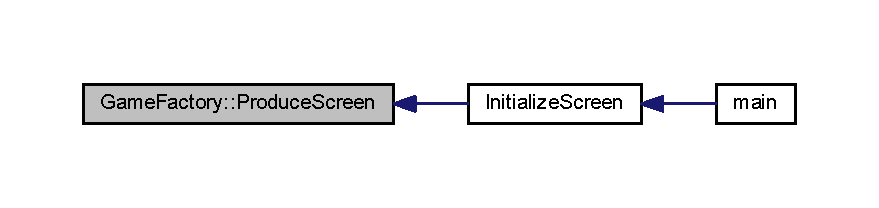
\includegraphics[width=350pt]{class_game_factory_ad293f5a8811d9106753916cef819fbce_icgraph}
\end{center}
\end{figure}


\hypertarget{class_game_factory_a3a20ae04c8ff992ad080b9742f5831c0}{\index{Game\-Factory@{Game\-Factory}!Register\-Layer\-Producer@{Register\-Layer\-Producer}}
\index{Register\-Layer\-Producer@{Register\-Layer\-Producer}!GameFactory@{Game\-Factory}}
\subsubsection[{Register\-Layer\-Producer}]{\setlength{\rightskip}{0pt plus 5cm}void Game\-Factory\-::\-Register\-Layer\-Producer (
\begin{DoxyParamCaption}
\item[{std\-::string}]{Name, }
\item[{{\bf Layer\-Producer} $\ast$}]{producer}
\end{DoxyParamCaption}
)}}\label{class_game_factory_a3a20ae04c8ff992ad080b9742f5831c0}


Here is the caller graph for this function\-:\nopagebreak
\begin{figure}[H]
\begin{center}
\leavevmode
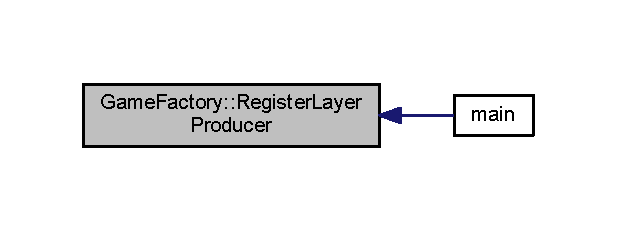
\includegraphics[width=296pt]{class_game_factory_a3a20ae04c8ff992ad080b9742f5831c0_icgraph}
\end{center}
\end{figure}


\hypertarget{class_game_factory_a77df8b5e97869b7d7b667c0852191e20}{\index{Game\-Factory@{Game\-Factory}!Register\-Object\-Producer@{Register\-Object\-Producer}}
\index{Register\-Object\-Producer@{Register\-Object\-Producer}!GameFactory@{Game\-Factory}}
\subsubsection[{Register\-Object\-Producer}]{\setlength{\rightskip}{0pt plus 5cm}void Game\-Factory\-::\-Register\-Object\-Producer (
\begin{DoxyParamCaption}
\item[{std\-::string}]{Name, }
\item[{{\bf Game\-Object\-Producer} $\ast$}]{producer}
\end{DoxyParamCaption}
)}}\label{class_game_factory_a77df8b5e97869b7d7b667c0852191e20}


Here is the caller graph for this function\-:\nopagebreak
\begin{figure}[H]
\begin{center}
\leavevmode
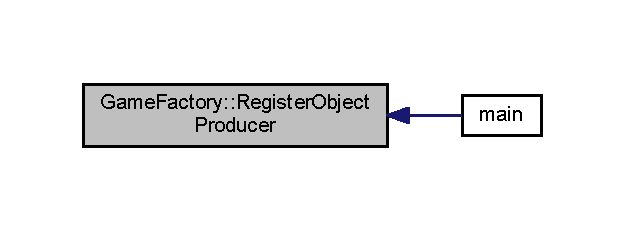
\includegraphics[width=300pt]{class_game_factory_a77df8b5e97869b7d7b667c0852191e20_icgraph}
\end{center}
\end{figure}


\hypertarget{class_game_factory_ad3c85f8654dd2c3aeb7a2b17df05cceb}{\index{Game\-Factory@{Game\-Factory}!Register\-Screen\-Producer@{Register\-Screen\-Producer}}
\index{Register\-Screen\-Producer@{Register\-Screen\-Producer}!GameFactory@{Game\-Factory}}
\subsubsection[{Register\-Screen\-Producer}]{\setlength{\rightskip}{0pt plus 5cm}void Game\-Factory\-::\-Register\-Screen\-Producer (
\begin{DoxyParamCaption}
\item[{std\-::string}]{Name, }
\item[{{\bf Game\-Screen\-Producer} $\ast$}]{producer}
\end{DoxyParamCaption}
)}}\label{class_game_factory_ad3c85f8654dd2c3aeb7a2b17df05cceb}


Here is the caller graph for this function\-:\nopagebreak
\begin{figure}[H]
\begin{center}
\leavevmode
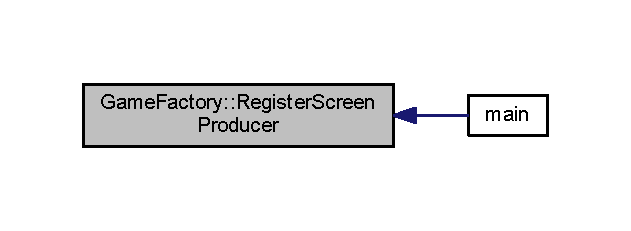
\includegraphics[width=303pt]{class_game_factory_ad3c85f8654dd2c3aeb7a2b17df05cceb_icgraph}
\end{center}
\end{figure}




\subsection{Member Data Documentation}
\hypertarget{class_game_factory_a77496a7ea1e2fa54acb18c499b3bd3bb}{\index{Game\-Factory@{Game\-Factory}!Chunks@{Chunks}}
\index{Chunks@{Chunks}!GameFactory@{Game\-Factory}}
\subsubsection[{Chunks}]{\setlength{\rightskip}{0pt plus 5cm}std\-::list$<${\bf Chunk} $\ast$$>$ Game\-Factory\-::\-Chunks\hspace{0.3cm}{\ttfamily [private]}}}\label{class_game_factory_a77496a7ea1e2fa54acb18c499b3bd3bb}
\hypertarget{class_game_factory_a90fc6360610babaf3d2d880f782772b3}{\index{Game\-Factory@{Game\-Factory}!Components@{Components}}
\index{Components@{Components}!GameFactory@{Game\-Factory}}
\subsubsection[{Components}]{\setlength{\rightskip}{0pt plus 5cm}std\-::list$<${\bf Game\-Component} $\ast$ $>$ Game\-Factory\-::\-Components\hspace{0.3cm}{\ttfamily [private]}}}\label{class_game_factory_a90fc6360610babaf3d2d880f782772b3}
\hypertarget{class_game_factory_adfadca1996a3982f4b45c67ced1520f2}{\index{Game\-Factory@{Game\-Factory}!Layer\-Producers@{Layer\-Producers}}
\index{Layer\-Producers@{Layer\-Producers}!GameFactory@{Game\-Factory}}
\subsubsection[{Layer\-Producers}]{\setlength{\rightskip}{0pt plus 5cm}std\-::map$<$std\-::string, {\bf Layer\-Producer} $\ast$$>$ Game\-Factory\-::\-Layer\-Producers\hspace{0.3cm}{\ttfamily [private]}}}\label{class_game_factory_adfadca1996a3982f4b45c67ced1520f2}
\hypertarget{class_game_factory_a7ab6a968cb7af49813407fe66927c126}{\index{Game\-Factory@{Game\-Factory}!Layers@{Layers}}
\index{Layers@{Layers}!GameFactory@{Game\-Factory}}
\subsubsection[{Layers}]{\setlength{\rightskip}{0pt plus 5cm}std\-::list$<${\bf Layer} $\ast$$>$ Game\-Factory\-::\-Layers\hspace{0.3cm}{\ttfamily [private]}}}\label{class_game_factory_a7ab6a968cb7af49813407fe66927c126}
\hypertarget{class_game_factory_ab72819fc3f241243d44827f75e0a2886}{\index{Game\-Factory@{Game\-Factory}!Object\-Producers@{Object\-Producers}}
\index{Object\-Producers@{Object\-Producers}!GameFactory@{Game\-Factory}}
\subsubsection[{Object\-Producers}]{\setlength{\rightskip}{0pt plus 5cm}std\-::map$<$std\-::string, {\bf Game\-Object\-Producer} $\ast$$>$ Game\-Factory\-::\-Object\-Producers\hspace{0.3cm}{\ttfamily [private]}}}\label{class_game_factory_ab72819fc3f241243d44827f75e0a2886}
\hypertarget{class_game_factory_aa65ba67e6c3fc56ec228c801e02352c8}{\index{Game\-Factory@{Game\-Factory}!Screen\-Producers@{Screen\-Producers}}
\index{Screen\-Producers@{Screen\-Producers}!GameFactory@{Game\-Factory}}
\subsubsection[{Screen\-Producers}]{\setlength{\rightskip}{0pt plus 5cm}std\-::map$<$std\-::string, {\bf Game\-Screen\-Producer} $\ast$$>$ Game\-Factory\-::\-Screen\-Producers\hspace{0.3cm}{\ttfamily [private]}}}\label{class_game_factory_aa65ba67e6c3fc56ec228c801e02352c8}
\hypertarget{class_game_factory_a16a8135f6d6b1b60c0d08b39340b34cc}{\index{Game\-Factory@{Game\-Factory}!Screens@{Screens}}
\index{Screens@{Screens}!GameFactory@{Game\-Factory}}
\subsubsection[{Screens}]{\setlength{\rightskip}{0pt plus 5cm}std\-::list$<${\bf Game\-Screen} $\ast$$>$ Game\-Factory\-::\-Screens\hspace{0.3cm}{\ttfamily [private]}}}\label{class_game_factory_a16a8135f6d6b1b60c0d08b39340b34cc}


The documentation for this class was generated from the following files\-:\begin{DoxyCompactItemize}
\item 
D\-:/\-Users/tom/\-Documents/\-Visual Studio 2013/\-Projects/\-Revelatorframework/\-Revelator\-Framework\-\_\-\-A\-P\-I/\hyperlink{_game_factory_8hpp}{Game\-Factory.\-hpp}\item 
D\-:/\-Users/tom/\-Documents/\-Visual Studio 2013/\-Projects/\-Revelatorframework/\-Revelator\-Framework\-\_\-\-A\-P\-I/\hyperlink{_game_factory_8cpp}{Game\-Factory.\-cpp}\end{DoxyCompactItemize}

\hypertarget{class_game_object_producer}{\section{Game\-Object\-Producer Class Reference}
\label{class_game_object_producer}\index{Game\-Object\-Producer@{Game\-Object\-Producer}}
}


{\ttfamily \#include $<$Game\-Object\-Producer.\-hpp$>$}



Inheritance diagram for Game\-Object\-Producer\-:\nopagebreak
\begin{figure}[H]
\begin{center}
\leavevmode
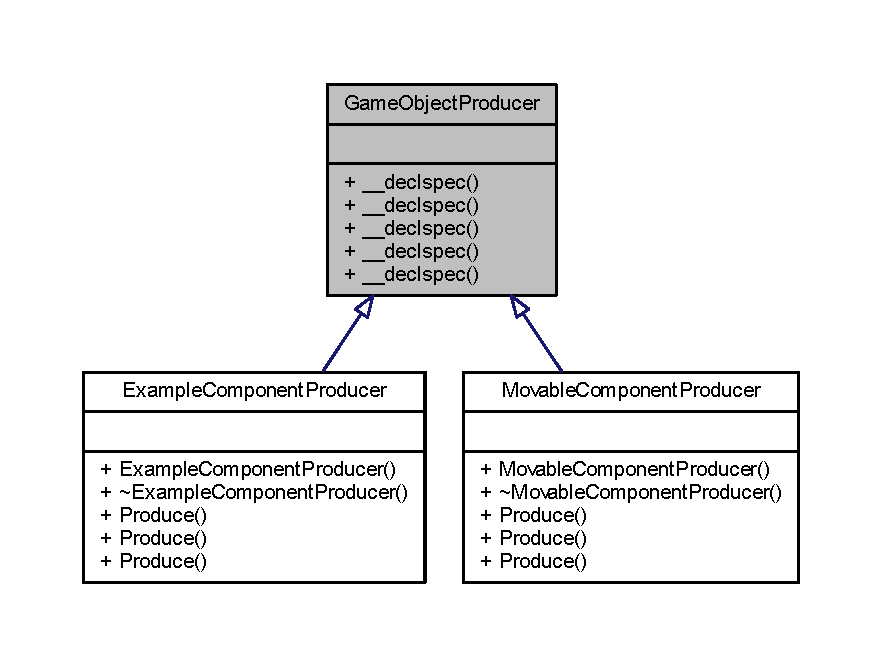
\includegraphics[width=350pt]{class_game_object_producer__inherit__graph}
\end{center}
\end{figure}


Collaboration diagram for Game\-Object\-Producer\-:\nopagebreak
\begin{figure}[H]
\begin{center}
\leavevmode
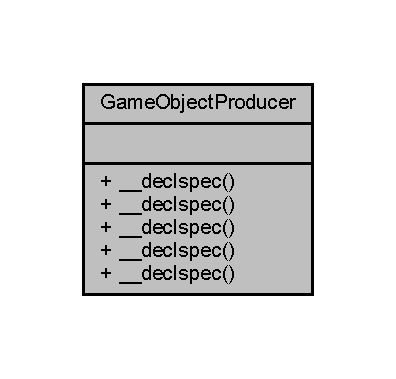
\includegraphics[width=211pt]{class_game_object_producer__coll__graph}
\end{center}
\end{figure}
\subsection*{Public Member Functions}
\begin{DoxyCompactItemize}
\item 
\hyperlink{class_game_object_producer_a38c70d3fba5ec49e549da7affbcf12d2}{Game\-Object\-Producer} ()
\item 
\hyperlink{class_game_object_producer_a77c862260fa83341a0b2fc8b1cad3ca5}{$\sim$\-Game\-Object\-Producer} ()
\item 
virtual \hyperlink{class_game_component}{Game\-Component} $\ast$ \hyperlink{class_game_object_producer_a10fa0f90fc8bb4720073818298ea16be}{Produce} ()=0
\item 
virtual \hyperlink{class_game_component}{Game\-Component} $\ast$ \hyperlink{class_game_object_producer_a2da5f02801c8b16cbf7b26daeade1513}{Produce} (\hyperlink{class_producer_package}{Producer\-Package} Package)=0
\item 
virtual \hyperlink{class_game_component}{Game\-Component} $\ast$ \hyperlink{class_game_object_producer_a572ce99f29ffaa2beb0231756281d403}{Produce} (\hyperlink{class_producer_package}{Producer\-Package} $\ast$Package)=0
\end{DoxyCompactItemize}


\subsection{Constructor \& Destructor Documentation}
\hypertarget{class_game_object_producer_a38c70d3fba5ec49e549da7affbcf12d2}{\index{Game\-Object\-Producer@{Game\-Object\-Producer}!Game\-Object\-Producer@{Game\-Object\-Producer}}
\index{Game\-Object\-Producer@{Game\-Object\-Producer}!GameObjectProducer@{Game\-Object\-Producer}}
\subsubsection[{Game\-Object\-Producer}]{\setlength{\rightskip}{0pt plus 5cm}Game\-Object\-Producer\-::\-Game\-Object\-Producer (
\begin{DoxyParamCaption}
{}
\end{DoxyParamCaption}
)}}\label{class_game_object_producer_a38c70d3fba5ec49e549da7affbcf12d2}
\hypertarget{class_game_object_producer_a77c862260fa83341a0b2fc8b1cad3ca5}{\index{Game\-Object\-Producer@{Game\-Object\-Producer}!$\sim$\-Game\-Object\-Producer@{$\sim$\-Game\-Object\-Producer}}
\index{$\sim$\-Game\-Object\-Producer@{$\sim$\-Game\-Object\-Producer}!GameObjectProducer@{Game\-Object\-Producer}}
\subsubsection[{$\sim$\-Game\-Object\-Producer}]{\setlength{\rightskip}{0pt plus 5cm}Game\-Object\-Producer\-::$\sim$\-Game\-Object\-Producer (
\begin{DoxyParamCaption}
{}
\end{DoxyParamCaption}
)}}\label{class_game_object_producer_a77c862260fa83341a0b2fc8b1cad3ca5}


\subsection{Member Function Documentation}
\hypertarget{class_game_object_producer_a10fa0f90fc8bb4720073818298ea16be}{\index{Game\-Object\-Producer@{Game\-Object\-Producer}!Produce@{Produce}}
\index{Produce@{Produce}!GameObjectProducer@{Game\-Object\-Producer}}
\subsubsection[{Produce}]{\setlength{\rightskip}{0pt plus 5cm}virtual {\bf Game\-Component}$\ast$ Game\-Object\-Producer\-::\-Produce (
\begin{DoxyParamCaption}
{}
\end{DoxyParamCaption}
)\hspace{0.3cm}{\ttfamily [pure virtual]}}}\label{class_game_object_producer_a10fa0f90fc8bb4720073818298ea16be}


Implemented in \hyperlink{class_example_component_producer_a63aba60e4b967000da407340505838de}{Example\-Component\-Producer}, and \hyperlink{class_movable_component_producer_afcef390a20c515da93a8ef1971e59b90}{Movable\-Component\-Producer}.

\hypertarget{class_game_object_producer_a2da5f02801c8b16cbf7b26daeade1513}{\index{Game\-Object\-Producer@{Game\-Object\-Producer}!Produce@{Produce}}
\index{Produce@{Produce}!GameObjectProducer@{Game\-Object\-Producer}}
\subsubsection[{Produce}]{\setlength{\rightskip}{0pt plus 5cm}virtual {\bf Game\-Component}$\ast$ Game\-Object\-Producer\-::\-Produce (
\begin{DoxyParamCaption}
\item[{{\bf Producer\-Package}}]{Package}
\end{DoxyParamCaption}
)\hspace{0.3cm}{\ttfamily [pure virtual]}}}\label{class_game_object_producer_a2da5f02801c8b16cbf7b26daeade1513}


Implemented in \hyperlink{class_example_component_producer_aeb985b69039c1db83c5826c01f31f53c}{Example\-Component\-Producer}, and \hyperlink{class_movable_component_producer_a909d2617235b049286660251050e7e8b}{Movable\-Component\-Producer}.

\hypertarget{class_game_object_producer_a572ce99f29ffaa2beb0231756281d403}{\index{Game\-Object\-Producer@{Game\-Object\-Producer}!Produce@{Produce}}
\index{Produce@{Produce}!GameObjectProducer@{Game\-Object\-Producer}}
\subsubsection[{Produce}]{\setlength{\rightskip}{0pt plus 5cm}virtual {\bf Game\-Component}$\ast$ Game\-Object\-Producer\-::\-Produce (
\begin{DoxyParamCaption}
\item[{{\bf Producer\-Package} $\ast$}]{Package}
\end{DoxyParamCaption}
)\hspace{0.3cm}{\ttfamily [pure virtual]}}}\label{class_game_object_producer_a572ce99f29ffaa2beb0231756281d403}


Implemented in \hyperlink{class_example_component_producer_a177b5d9088f69aed43d10c9b2b8f2c01}{Example\-Component\-Producer}, and \hyperlink{class_movable_component_producer_a1b83286374915b711d4b8f55cc024cbc}{Movable\-Component\-Producer}.



The documentation for this class was generated from the following files\-:\begin{DoxyCompactItemize}
\item 
D\-:/\-Users/tom/\-Documents/\-Visual Studio 2013/\-Projects/\-Revelatorframework/\-Revelator\-Framework\-\_\-\-A\-P\-I/\hyperlink{_game_object_producer_8hpp}{Game\-Object\-Producer.\-hpp}\item 
D\-:/\-Users/tom/\-Documents/\-Visual Studio 2013/\-Projects/\-Revelatorframework/\-Revelator\-Framework\-\_\-\-A\-P\-I/\hyperlink{_game_object_producer_8cpp}{Game\-Object\-Producer.\-cpp}\end{DoxyCompactItemize}

\hypertarget{class_game_screen}{\section{Game\-Screen Class Reference}
\label{class_game_screen}\index{Game\-Screen@{Game\-Screen}}
}


{\ttfamily \#include $<$Game\-Screen.\-hpp$>$}



Inheritance diagram for Game\-Screen\-:\nopagebreak
\begin{figure}[H]
\begin{center}
\leavevmode
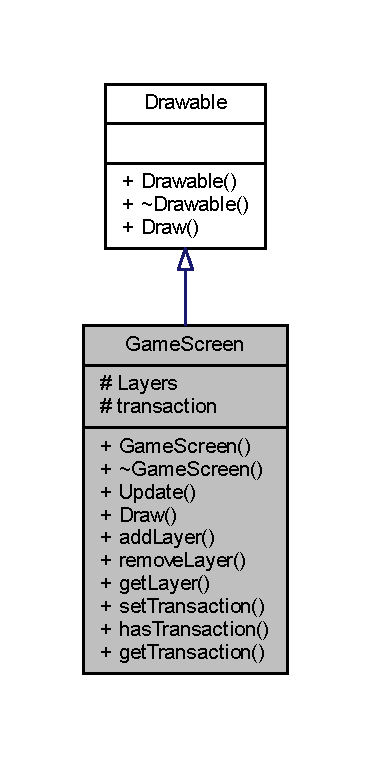
\includegraphics[width=205pt]{class_game_screen__inherit__graph}
\end{center}
\end{figure}


Collaboration diagram for Game\-Screen\-:\nopagebreak
\begin{figure}[H]
\begin{center}
\leavevmode
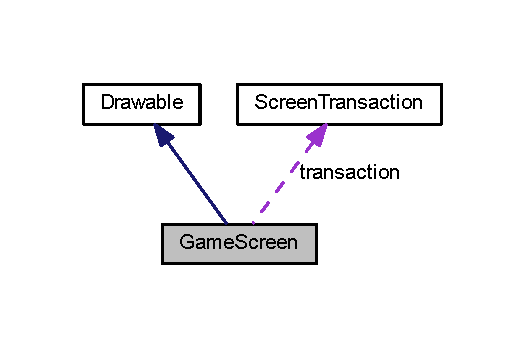
\includegraphics[width=161pt]{class_game_screen__coll__graph}
\end{center}
\end{figure}
\subsection*{Public Member Functions}
\begin{DoxyCompactItemize}
\item 
\hyperlink{class_game_screen_a41fb99405265eadec9712c99673a05f1}{\-\_\-\-\_\-declspec} (dllexport) \hyperlink{class_game_screen}{Game\-Screen}()
\item 
\hyperlink{class_game_screen_a940d1b9790ff4b737ee4c521d10a5e08}{\-\_\-\-\_\-declspec} (dllexport)$\sim$\hyperlink{class_game_screen}{Game\-Screen}()
\item 
\hyperlink{class_game_screen_a902bce77e2df723b9547d6364b5aaadf}{\-\_\-\-\_\-declspec} (dllexport) void Update(const \hyperlink{class_update_data}{Update\-Data} \&updateobject)
\item 
\hyperlink{class_game_screen_a03f75f898e71457324bd5f2cea6fc8a2}{\-\_\-\-\_\-declspec} (dllexport) virtual void Entry(\hyperlink{class_entry_object}{Entry\-Object} object)=0
\end{DoxyCompactItemize}
\subsection*{Private Attributes}
\begin{DoxyCompactItemize}
\item 
std\-::map$<$ std\-::string, \hyperlink{class_layer}{Layer} $\ast$ $>$ \hyperlink{class_game_screen_ab134d175092c247558838f11d66e9493}{Layers}
\end{DoxyCompactItemize}


\subsection{Member Function Documentation}
\hypertarget{class_game_screen_a41fb99405265eadec9712c99673a05f1}{\index{Game\-Screen@{Game\-Screen}!\-\_\-\-\_\-declspec@{\-\_\-\-\_\-declspec}}
\index{\-\_\-\-\_\-declspec@{\-\_\-\-\_\-declspec}!GameScreen@{Game\-Screen}}
\subsubsection[{\-\_\-\-\_\-declspec}]{\setlength{\rightskip}{0pt plus 5cm}Game\-Screen\-::\-\_\-\-\_\-declspec (
\begin{DoxyParamCaption}
\item[{dllexport}]{}
\end{DoxyParamCaption}
)}}\label{class_game_screen_a41fb99405265eadec9712c99673a05f1}
\hypertarget{class_game_screen_a940d1b9790ff4b737ee4c521d10a5e08}{\index{Game\-Screen@{Game\-Screen}!\-\_\-\-\_\-declspec@{\-\_\-\-\_\-declspec}}
\index{\-\_\-\-\_\-declspec@{\-\_\-\-\_\-declspec}!GameScreen@{Game\-Screen}}
\subsubsection[{\-\_\-\-\_\-declspec}]{\setlength{\rightskip}{0pt plus 5cm}Game\-Screen\-::\-\_\-\-\_\-declspec (
\begin{DoxyParamCaption}
\item[{dllexport}]{}
\end{DoxyParamCaption}
)}}\label{class_game_screen_a940d1b9790ff4b737ee4c521d10a5e08}
\hypertarget{class_game_screen_a902bce77e2df723b9547d6364b5aaadf}{\index{Game\-Screen@{Game\-Screen}!\-\_\-\-\_\-declspec@{\-\_\-\-\_\-declspec}}
\index{\-\_\-\-\_\-declspec@{\-\_\-\-\_\-declspec}!GameScreen@{Game\-Screen}}
\subsubsection[{\-\_\-\-\_\-declspec}]{\setlength{\rightskip}{0pt plus 5cm}Game\-Screen\-::\-\_\-\-\_\-declspec (
\begin{DoxyParamCaption}
\item[{dllexport}]{}
\end{DoxyParamCaption}
) const}}\label{class_game_screen_a902bce77e2df723b9547d6364b5aaadf}
\hypertarget{class_game_screen_a03f75f898e71457324bd5f2cea6fc8a2}{\index{Game\-Screen@{Game\-Screen}!\-\_\-\-\_\-declspec@{\-\_\-\-\_\-declspec}}
\index{\-\_\-\-\_\-declspec@{\-\_\-\-\_\-declspec}!GameScreen@{Game\-Screen}}
\subsubsection[{\-\_\-\-\_\-declspec}]{\setlength{\rightskip}{0pt plus 5cm}Game\-Screen\-::\-\_\-\-\_\-declspec (
\begin{DoxyParamCaption}
\item[{dllexport}]{}
\end{DoxyParamCaption}
)\hspace{0.3cm}{\ttfamily [pure virtual]}}}\label{class_game_screen_a03f75f898e71457324bd5f2cea6fc8a2}


\subsection{Member Data Documentation}
\hypertarget{class_game_screen_ab134d175092c247558838f11d66e9493}{\index{Game\-Screen@{Game\-Screen}!Layers@{Layers}}
\index{Layers@{Layers}!GameScreen@{Game\-Screen}}
\subsubsection[{Layers}]{\setlength{\rightskip}{0pt plus 5cm}std\-::map$<$std\-::string, {\bf Layer}$\ast$$>$ Game\-Screen\-::\-Layers\hspace{0.3cm}{\ttfamily [private]}}}\label{class_game_screen_ab134d175092c247558838f11d66e9493}


The documentation for this class was generated from the following file\-:\begin{DoxyCompactItemize}
\item 
D\-:/\-Users/tom/\-Documents/\-Visual Studio 2013/\-Projects/\-Revelatorframework/\-Revelator\-Framework\-\_\-\-A\-P\-I/\hyperlink{_game_screen_8hpp}{Game\-Screen.\-hpp}\end{DoxyCompactItemize}

\hypertarget{class_game_screen_producer}{\section{Game\-Screen\-Producer Class Reference}
\label{class_game_screen_producer}\index{Game\-Screen\-Producer@{Game\-Screen\-Producer}}
}


{\ttfamily \#include $<$Game\-Screen\-Producer.\-hpp$>$}



Inheritance diagram for Game\-Screen\-Producer\-:\nopagebreak
\begin{figure}[H]
\begin{center}
\leavevmode
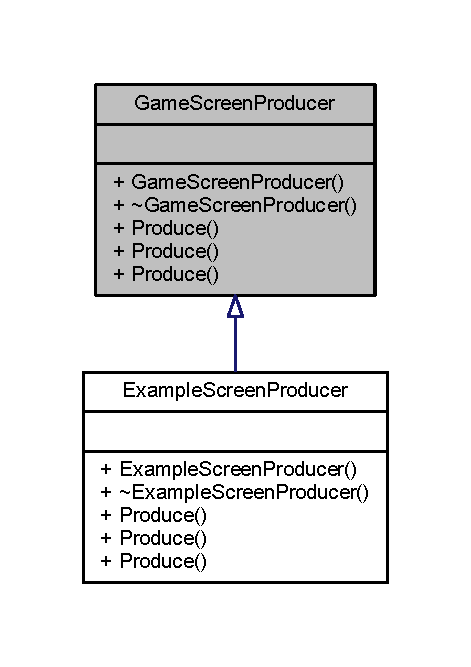
\includegraphics[width=226pt]{class_game_screen_producer__inherit__graph}
\end{center}
\end{figure}


Collaboration diagram for Game\-Screen\-Producer\-:\nopagebreak
\begin{figure}[H]
\begin{center}
\leavevmode
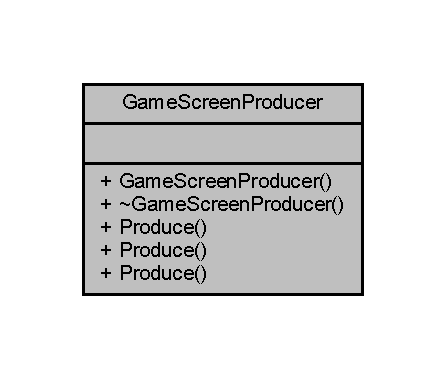
\includegraphics[width=193pt]{class_game_screen_producer__coll__graph}
\end{center}
\end{figure}
\subsection*{Public Member Functions}
\begin{DoxyCompactItemize}
\item 
\hyperlink{class_game_screen_producer_a763fe68a79dccbe05e843124ad62eb36}{\-\_\-\-\_\-declspec} (dllexport) \hyperlink{class_game_screen_producer}{Game\-Screen\-Producer}()
\item 
\hyperlink{class_game_screen_producer_a3b4fd8a10b2a9e9ed2b5816d464cb3bb}{\-\_\-\-\_\-declspec} (dllexport)$\sim$\hyperlink{class_game_screen_producer}{Game\-Screen\-Producer}()
\item 
\hyperlink{class_game_screen_producer_a56e7ccd432601c6a28f714201dabc46f}{\-\_\-\-\_\-declspec} (dllexport) virtual \hyperlink{class_game_screen}{Game\-Screen} $\ast$Produce()=0
\item 
\hyperlink{class_game_screen_producer_a7a18ea24631d12709cdf30f692802ba2}{\-\_\-\-\_\-declspec} (dllexport) virtual \hyperlink{class_game_screen}{Game\-Screen} $\ast$Produce(\hyperlink{class_producer_package}{Producer\-Package} Package)=0
\item 
\hyperlink{class_game_screen_producer_a86b3d35e0edf3bdc411bb9cb79ea2647}{\-\_\-\-\_\-declspec} (dllexport) virtual \hyperlink{class_game_screen}{Game\-Screen} $\ast$Produce(\hyperlink{class_producer_package}{Producer\-Package} $\ast$Package)=0
\end{DoxyCompactItemize}


\subsection{Member Function Documentation}
\hypertarget{class_game_screen_producer_a763fe68a79dccbe05e843124ad62eb36}{\index{Game\-Screen\-Producer@{Game\-Screen\-Producer}!\-\_\-\-\_\-declspec@{\-\_\-\-\_\-declspec}}
\index{\-\_\-\-\_\-declspec@{\-\_\-\-\_\-declspec}!GameScreenProducer@{Game\-Screen\-Producer}}
\subsubsection[{\-\_\-\-\_\-declspec}]{\setlength{\rightskip}{0pt plus 5cm}Game\-Screen\-Producer\-::\-\_\-\-\_\-declspec (
\begin{DoxyParamCaption}
\item[{dllexport}]{}
\end{DoxyParamCaption}
)}}\label{class_game_screen_producer_a763fe68a79dccbe05e843124ad62eb36}
\hypertarget{class_game_screen_producer_a3b4fd8a10b2a9e9ed2b5816d464cb3bb}{\index{Game\-Screen\-Producer@{Game\-Screen\-Producer}!\-\_\-\-\_\-declspec@{\-\_\-\-\_\-declspec}}
\index{\-\_\-\-\_\-declspec@{\-\_\-\-\_\-declspec}!GameScreenProducer@{Game\-Screen\-Producer}}
\subsubsection[{\-\_\-\-\_\-declspec}]{\setlength{\rightskip}{0pt plus 5cm}Game\-Screen\-Producer\-::\-\_\-\-\_\-declspec (
\begin{DoxyParamCaption}
\item[{dllexport}]{}
\end{DoxyParamCaption}
)}}\label{class_game_screen_producer_a3b4fd8a10b2a9e9ed2b5816d464cb3bb}
\hypertarget{class_game_screen_producer_a56e7ccd432601c6a28f714201dabc46f}{\index{Game\-Screen\-Producer@{Game\-Screen\-Producer}!\-\_\-\-\_\-declspec@{\-\_\-\-\_\-declspec}}
\index{\-\_\-\-\_\-declspec@{\-\_\-\-\_\-declspec}!GameScreenProducer@{Game\-Screen\-Producer}}
\subsubsection[{\-\_\-\-\_\-declspec}]{\setlength{\rightskip}{0pt plus 5cm}Game\-Screen\-Producer\-::\-\_\-\-\_\-declspec (
\begin{DoxyParamCaption}
\item[{dllexport}]{}
\end{DoxyParamCaption}
)\hspace{0.3cm}{\ttfamily [pure virtual]}}}\label{class_game_screen_producer_a56e7ccd432601c6a28f714201dabc46f}
\hypertarget{class_game_screen_producer_a7a18ea24631d12709cdf30f692802ba2}{\index{Game\-Screen\-Producer@{Game\-Screen\-Producer}!\-\_\-\-\_\-declspec@{\-\_\-\-\_\-declspec}}
\index{\-\_\-\-\_\-declspec@{\-\_\-\-\_\-declspec}!GameScreenProducer@{Game\-Screen\-Producer}}
\subsubsection[{\-\_\-\-\_\-declspec}]{\setlength{\rightskip}{0pt plus 5cm}Game\-Screen\-Producer\-::\-\_\-\-\_\-declspec (
\begin{DoxyParamCaption}
\item[{dllexport}]{}
\end{DoxyParamCaption}
)\hspace{0.3cm}{\ttfamily [pure virtual]}}}\label{class_game_screen_producer_a7a18ea24631d12709cdf30f692802ba2}
\hypertarget{class_game_screen_producer_a86b3d35e0edf3bdc411bb9cb79ea2647}{\index{Game\-Screen\-Producer@{Game\-Screen\-Producer}!\-\_\-\-\_\-declspec@{\-\_\-\-\_\-declspec}}
\index{\-\_\-\-\_\-declspec@{\-\_\-\-\_\-declspec}!GameScreenProducer@{Game\-Screen\-Producer}}
\subsubsection[{\-\_\-\-\_\-declspec}]{\setlength{\rightskip}{0pt plus 5cm}Game\-Screen\-Producer\-::\-\_\-\-\_\-declspec (
\begin{DoxyParamCaption}
\item[{dllexport}]{}
\end{DoxyParamCaption}
)\hspace{0.3cm}{\ttfamily [pure virtual]}}}\label{class_game_screen_producer_a86b3d35e0edf3bdc411bb9cb79ea2647}


The documentation for this class was generated from the following file\-:\begin{DoxyCompactItemize}
\item 
D\-:/\-Users/tom/\-Documents/\-Visual Studio 2013/\-Projects/\-Revelatorframework/\-Revelator\-Framework\-\_\-\-A\-P\-I/\hyperlink{_game_screen_producer_8hpp}{Game\-Screen\-Producer.\-hpp}\end{DoxyCompactItemize}

\hypertarget{class_keyboard}{\section{Keyboard Class Reference}
\label{class_keyboard}\index{Keyboard@{Keyboard}}
}


{\ttfamily \#include $<$Keyboard.\-hpp$>$}



Collaboration diagram for Keyboard\-:\nopagebreak
\begin{figure}[H]
\begin{center}
\leavevmode
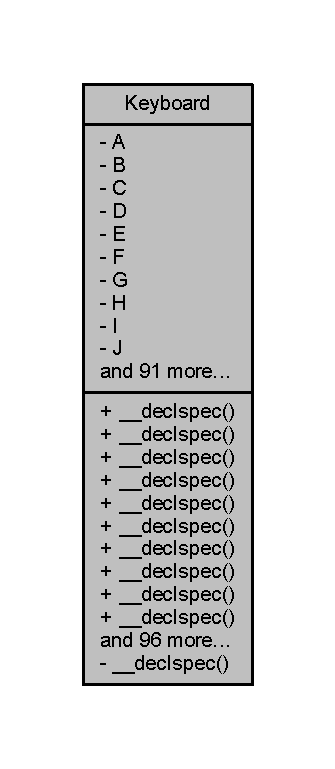
\includegraphics[width=162pt]{class_keyboard__coll__graph}
\end{center}
\end{figure}
\subsection*{Public Member Functions}
\begin{DoxyCompactItemize}
\item 
\hyperlink{class_keyboard_af6a99ec66c8c722a45b967bf79167038}{$\sim$\-Keyboard} ()
\item 
\hyperlink{class_keyboard_a6d15d5289af582f6f247ae333034db02}{Keyboard} (const \hyperlink{class_keyboard}{Keyboard} \&keyboard)=delete
\item 
\hyperlink{class_keyboard}{Keyboard} \& \hyperlink{class_keyboard_a92fe736c2e88e5ed828dd985c857da0a}{operator=} (const \hyperlink{class_keyboard}{Keyboard} \&keyboard)=delete
\item 
void \hyperlink{class_keyboard_a6410f07ddc53561a82d5328d8b330aab}{update} ()
\item 
bool \hyperlink{class_keyboard_acb69c710e18e3578fa5ed66e07e6b766}{get\-A} ()
\item 
bool \hyperlink{class_keyboard_abe467d1841c9c0b89c5856e9b3259980}{get\-B} ()
\item 
bool \hyperlink{class_keyboard_ae14994ae9d4a753c90511eee46f9b8eb}{get\-C} ()
\item 
bool \hyperlink{class_keyboard_ab9e7561799ddc1941283333dcd50c5e1}{get\-D} ()
\item 
bool \hyperlink{class_keyboard_ac1fbe5b7e31739174b7cd810521a2e9d}{get\-E} ()
\item 
bool \hyperlink{class_keyboard_a6fec87afe52371c8a264745a5c487d06}{get\-F} ()
\item 
bool \hyperlink{class_keyboard_a31aae98dfbc61407fa004ae2f7595452}{get\-G} ()
\item 
bool \hyperlink{class_keyboard_a0deba682104bf09a85d23ab4085d53f8}{get\-H} ()
\item 
bool \hyperlink{class_keyboard_a533b9c9ea72e078a6ed1081e0293a457}{get\-I} ()
\item 
bool \hyperlink{class_keyboard_a47d68d720a385e1b58d28ecffbf97964}{get\-J} ()
\item 
bool \hyperlink{class_keyboard_ac512b5cbd9f8c229a6a4c81c0ca12f91}{get\-K} ()
\item 
bool \hyperlink{class_keyboard_a0bb30d06c8ed37ae9e0e55135f2b7170}{get\-L} ()
\item 
bool \hyperlink{class_keyboard_a06888fa46c0dc92103a4d7416bfb474e}{get\-M} ()
\item 
bool \hyperlink{class_keyboard_a0b5d31dc62328f59af7ff137de090818}{get\-N} ()
\item 
bool \hyperlink{class_keyboard_a1d52718b43926378944d3ec1ab4ef245}{get\-O} ()
\item 
bool \hyperlink{class_keyboard_a9c96638ce77e4a6bfee3f7c18bcb9b63}{get\-P} ()
\item 
bool \hyperlink{class_keyboard_ad3960e897150ae3121301bff4381e56a}{get\-Q} ()
\item 
bool \hyperlink{class_keyboard_a42d4db82a7ea40418c831a8d68719ca6}{get\-R} ()
\item 
bool \hyperlink{class_keyboard_a38c76aa89c02ba8a98b81299278f813c}{get\-S} ()
\item 
bool \hyperlink{class_keyboard_a7d2d380e26575a378431edf4a9fe9e5b}{get\-T} ()
\item 
bool \hyperlink{class_keyboard_a217742d32bedc411969d0b9fc8695d0c}{get\-U} ()
\item 
bool \hyperlink{class_keyboard_a742945eb88fc6f0a080b4caea661a64f}{get\-V} ()
\item 
bool \hyperlink{class_keyboard_abbfd652fcf142863462910076a5298dd}{get\-W} ()
\item 
bool \hyperlink{class_keyboard_afa058729c91b1233101d408d77985f87}{get\-X} ()
\item 
bool \hyperlink{class_keyboard_ac15b70f1cb6b0cbecdeed7c363922411}{get\-Y} ()
\item 
bool \hyperlink{class_keyboard_ac9855a7877c01f7d29f4a4d10217bfc1}{get\-Z} ()
\item 
bool \hyperlink{class_keyboard_a1c5ecb4909477ec4a5173353171912bd}{get\-Num0} ()
\item 
bool \hyperlink{class_keyboard_a27d7ebfb0172d399530245cd00243fb0}{get\-Num1} ()
\item 
bool \hyperlink{class_keyboard_a6e5e05e63ae1cfb59ca375b05dcbe688}{get\-Num2} ()
\item 
bool \hyperlink{class_keyboard_acb62d27041dd2d39968c2d2fe424155d}{get\-Num3} ()
\item 
bool \hyperlink{class_keyboard_adf405bac73bbe34b554b452ce531fd09}{get\-Num4} ()
\item 
bool \hyperlink{class_keyboard_a5a172c6bab05bb95d20ddb80a2d23d95}{get\-Num5} ()
\item 
bool \hyperlink{class_keyboard_af08887ae78e829222420acada6707ac8}{get\-Num6} ()
\item 
bool \hyperlink{class_keyboard_a08d1067ac6b0c8836f01608e60842625}{get\-Num7} ()
\item 
bool \hyperlink{class_keyboard_af0e119a74e4fcca0bbda53d885bd4245}{get\-Num8} ()
\item 
bool \hyperlink{class_keyboard_a0e1c476a2d5e4c9c0f9a7a2c97356bfa}{get\-Num9} ()
\item 
bool \hyperlink{class_keyboard_a994ab28476380c8233e80cb0f349bdb8}{get\-Escape} ()
\item 
bool \hyperlink{class_keyboard_a5f60b99ed9f012e78629acfe1f795be3}{get\-L\-Control} ()
\item 
bool \hyperlink{class_keyboard_a410f25adf92d4120faeab8334ededba9}{get\-L\-Shift} ()
\item 
bool \hyperlink{class_keyboard_a2ad4b6abd18ebd2a6c69da2de338265c}{get\-L\-Alt} ()
\item 
bool \hyperlink{class_keyboard_ab58d4d9bb82bf64de46fa1792fd80086}{get\-L\-System} ()
\item 
bool \hyperlink{class_keyboard_a428d96963222eff1fefb15198403c14c}{get\-R\-Control} ()
\item 
bool \hyperlink{class_keyboard_a412703b9a1957036c6ef559e804aed91}{get\-R\-Shift} ()
\item 
bool \hyperlink{class_keyboard_a670aae3f40bf02f26fb966f25ff06234}{get\-R\-Alt} ()
\item 
bool \hyperlink{class_keyboard_a8659cc000033848acae7c18683886a92}{get\-R\-System} ()
\item 
bool \hyperlink{class_keyboard_ad5c31b46ab392c8cfeb4f060ce346e22}{get\-Menu} ()
\item 
bool \hyperlink{class_keyboard_a62d0bd6e13a7c2ef5d70f0c63c7b6104}{get\-L\-Bracket} ()
\item 
bool \hyperlink{class_keyboard_a065e43a5ece4a6a8790e3f8a8817ea23}{get\-R\-Bracket} ()
\item 
bool \hyperlink{class_keyboard_add5ee27f0c650e722f0c6666ed57b022}{get\-Semi\-Colon} ()
\item 
bool \hyperlink{class_keyboard_aec17bf7d0b87ccdd5020ab9fa3b94413}{get\-Comma} ()
\item 
bool \hyperlink{class_keyboard_a6fc2692d8e1006b086a82678aabdbad3}{get\-Period} ()
\item 
bool \hyperlink{class_keyboard_a09b58b89fb75696031d097278eac0ec7}{get\-Quote} ()
\item 
bool \hyperlink{class_keyboard_af84d491804fc8be29f3646251faf1611}{get\-Slash} ()
\item 
bool \hyperlink{class_keyboard_a57019e241d4e3413ee6bd68e6a6a3d79}{get\-Back\-Slash} ()
\item 
bool \hyperlink{class_keyboard_ab0e0b87609daf296416a181d2aa327cb}{get\-Tilde} ()
\item 
bool \hyperlink{class_keyboard_ab33d990d565c0e9e6de234c2ccd847fd}{get\-Equal} ()
\item 
bool \hyperlink{class_keyboard_a2b629ac3f7efb81b4dd6091894261900}{get\-Dash} ()
\item 
bool \hyperlink{class_keyboard_ab8dc7b677742e216c75f4e4c739bed12}{get\-Space} ()
\item 
bool \hyperlink{class_keyboard_a04482f34bbd2f5d2463acbe07e8b2e56}{get\-Return} ()
\item 
bool \hyperlink{class_keyboard_ab425b0b196ffde8d878097b71884702a}{get\-Back\-Space} ()
\item 
bool \hyperlink{class_keyboard_a0d775a126b75313576041cdaa1ce5fde}{get\-Tab} ()
\item 
bool \hyperlink{class_keyboard_a6da15fa7a8b213e66c97b32411bd8c5a}{get\-Page\-Up} ()
\item 
bool \hyperlink{class_keyboard_ac2a759e6f55eb9faf0fe483df06f0adb}{get\-Page\-Down} ()
\item 
bool \hyperlink{class_keyboard_adbbf01e7ad22f2c1f1253053a90524c2}{get\-End} ()
\item 
bool \hyperlink{class_keyboard_aaa8d566aa66eddbe2a3a3ce5565cb34f}{get\-Home} ()
\item 
bool \hyperlink{class_keyboard_a78814c54bdbb71866480a73bec46c1da}{get\-Insert} ()
\item 
bool \hyperlink{class_keyboard_aa65d80a94c32f9a3180d4c73049165fd}{get\-Delete} ()
\item 
bool \hyperlink{class_keyboard_aafc539a77070e0d53551199bf69877d8}{get\-Add} ()
\item 
bool \hyperlink{class_keyboard_ab251d50b95897e7c69219ea2d3fe1e97}{get\-Subtract} ()
\item 
bool \hyperlink{class_keyboard_a9971de37c9040738efa45a0e51aee175}{get\-Multiply} ()
\item 
bool \hyperlink{class_keyboard_abca2a6295ec794e1547ced02396b4835}{get\-Divide} ()
\item 
bool \hyperlink{class_keyboard_ac8b072ea0e90e87b10470bc92cec1a5c}{get\-Left} ()
\item 
bool \hyperlink{class_keyboard_a33607f70dec11df2ea88dfe7e49d40ef}{get\-Right} ()
\item 
bool \hyperlink{class_keyboard_aeac99170e4a0b5a4a0b58beda53875d5}{get\-Up} ()
\item 
bool \hyperlink{class_keyboard_a9d07f97d9a6d654c768864fbd3beea23}{get\-Down} ()
\item 
bool \hyperlink{class_keyboard_a909c70a8e72b75c9515441651b88372d}{get\-Numpad0} ()
\item 
bool \hyperlink{class_keyboard_a1ea935eecc5f69b46898529d6e019d27}{get\-Numpad1} ()
\item 
bool \hyperlink{class_keyboard_a395b15a9fa1916d79bf5fc84f87f0919}{get\-Numpad2} ()
\item 
bool \hyperlink{class_keyboard_a650ce67f4890d668e58f8f2c459f345f}{get\-Numpad3} ()
\item 
bool \hyperlink{class_keyboard_a3d9b7aa434579001274e29919da7351c}{get\-Numpad4} ()
\item 
bool \hyperlink{class_keyboard_a39972d7e2eab16ac5af74a5ba6c0d7a2}{get\-Numpad5} ()
\item 
bool \hyperlink{class_keyboard_a72f11330e522fd2d8d6d096f703b717b}{get\-Numpad6} ()
\item 
bool \hyperlink{class_keyboard_a24ebd525127b9d17386a1e6267905ef5}{get\-Numpad7} ()
\item 
bool \hyperlink{class_keyboard_a181042ca4d186805ff9f3a6d36b14f1b}{get\-Numpad8} ()
\item 
bool \hyperlink{class_keyboard_a1dcfce958bfb7957b1d6b85706f9728f}{get\-Numpad9} ()
\item 
bool \hyperlink{class_keyboard_a89d9b338c53114a8a736b33e9767f72e}{get\-F1} ()
\item 
bool \hyperlink{class_keyboard_a2fec13e7b4db8d34fd460f178b14e54c}{get\-F2} ()
\item 
bool \hyperlink{class_keyboard_a82cc37753de536fed35da764e6c30d26}{get\-F3} ()
\item 
bool \hyperlink{class_keyboard_ac9c2d3a80291c00101e4d89661be33a8}{get\-F4} ()
\item 
bool \hyperlink{class_keyboard_ac10076d1fe94851272cc90cf6690b8cc}{get\-F5} ()
\item 
bool \hyperlink{class_keyboard_adc476a2af4f6ef9a983da62d8d2fed0a}{get\-F6} ()
\item 
bool \hyperlink{class_keyboard_a8e843446827b1c258aaff1d5c0ad0024}{get\-F7} ()
\item 
bool \hyperlink{class_keyboard_ae875c4c35788a819158e2c1a7628d8f6}{get\-F8} ()
\item 
bool \hyperlink{class_keyboard_a154b39d12c6f8cc1c5bfbbb5282bc7e3}{get\-F9} ()
\item 
bool \hyperlink{class_keyboard_ae8a49362a97f0f85ed9f9d4430d3ce39}{get\-F10} ()
\item 
bool \hyperlink{class_keyboard_a88608100c5a4e694922ce5054888407e}{get\-F11} ()
\item 
bool \hyperlink{class_keyboard_a322c334deaf0b92c93416816a482b6ba}{get\-F12} ()
\item 
bool \hyperlink{class_keyboard_abff30ad0570f44cb49f979b7f88f76ea}{get\-F13} ()
\item 
bool \hyperlink{class_keyboard_af1814f932c5b125d113c99a0879c22a0}{get\-F14} ()
\item 
bool \hyperlink{class_keyboard_a2d62f212870972657e5ae965a11df89d}{get\-F15} ()
\item 
bool \hyperlink{class_keyboard_a1bf2789c0743f4f00cb5778d62242315}{get\-Pause} ()
\end{DoxyCompactItemize}
\subsection*{Static Public Member Functions}
\begin{DoxyCompactItemize}
\item 
static \hyperlink{class_keyboard}{Keyboard} \& \hyperlink{class_keyboard_a09fc76a431abc21dba175b10bc4a1ec8}{get\-Instance} ()
\end{DoxyCompactItemize}
\subsection*{Private Member Functions}
\begin{DoxyCompactItemize}
\item 
\hyperlink{class_keyboard_ad6b0bb849d6bb7cdf63091e40b5f5f7f}{Keyboard} ()
\end{DoxyCompactItemize}
\subsection*{Private Attributes}
\begin{DoxyCompactItemize}
\item 
bool \hyperlink{class_keyboard_a33ee9c98d3b2426fec7b69fd4f42fb9a}{A}
\item 
bool \hyperlink{class_keyboard_a6386fea4a95993853302e9bafb520eca}{B}
\item 
bool \hyperlink{class_keyboard_a8e9a644f450a387c8b0becfec29e0eba}{C}
\item 
bool \hyperlink{class_keyboard_a913ff21c18119ddf7a4185c84e0e7449}{D}
\item 
bool \hyperlink{class_keyboard_a10f9fdb7927cb81bba0d054c26509a7a}{E}
\item 
bool \hyperlink{class_keyboard_af271aa6fd76947941d20934dc86a0bb2}{F}
\item 
bool \hyperlink{class_keyboard_a2c602997ff88ff6b54a696397e5478f9}{G}
\item 
bool \hyperlink{class_keyboard_a5756caddc794320748593954cbd35a2a}{H}
\item 
bool \hyperlink{class_keyboard_a59f5f1879a371a750deaef44730f6c8e}{I}
\item 
bool \hyperlink{class_keyboard_a79e10d1e2486a150419889ac513386b9}{J}
\item 
bool \hyperlink{class_keyboard_a805724edf1245e28598089225bcae72e}{K}
\item 
bool \hyperlink{class_keyboard_ad314cbbe55e6d9d699f9c4a3d673dc0e}{L}
\item 
bool \hyperlink{class_keyboard_a655e239c891a0c77273f5651f77d752b}{M}
\item 
bool \hyperlink{class_keyboard_a9c13f7665efcec0323466f50080dd90f}{N}
\item 
bool \hyperlink{class_keyboard_ac2ef655c59d2d20ca9ac14b38281bd2b}{O}
\item 
bool \hyperlink{class_keyboard_a0a1ccbf5bdd2ca101d91f6aeb12b0003}{P}
\item 
bool \hyperlink{class_keyboard_a73542918c6ffdd4915925fff6aea1eb5}{Q}
\item 
bool \hyperlink{class_keyboard_a43732e3f8a2a179490d70bbca9c9cbf7}{R}
\item 
bool \hyperlink{class_keyboard_aafafb740df9ac23e0fdbac7b85ca5902}{S}
\item 
bool \hyperlink{class_keyboard_a82a8270c2f89be1d02deff45e5b05423}{T}
\item 
bool \hyperlink{class_keyboard_a73a0cb0a587e4aea584d64486c95996b}{U}
\item 
bool \hyperlink{class_keyboard_ae41741f501d169e8671242bae37c608f}{V}
\item 
bool \hyperlink{class_keyboard_a7c1dbac444af2066b65cb5f73cfeb00e}{W}
\item 
bool \hyperlink{class_keyboard_afde15308c9554c8abaf8054b105b9507}{X}
\item 
bool \hyperlink{class_keyboard_a030813b88756995bdc8b577b3674dd0a}{Y}
\item 
bool \hyperlink{class_keyboard_abbae1e2f05e366553c81c136a0f3f970}{Z}
\item 
bool \hyperlink{class_keyboard_adcaa025a0862c4ef0b915a39f095f86c}{Num0}
\item 
bool \hyperlink{class_keyboard_a835bf1e4085d8f539a374f38fcf44a52}{Num1}
\item 
bool \hyperlink{class_keyboard_af4ec2c5721ec5c013867e16d3b37dd0b}{Num2}
\item 
bool \hyperlink{class_keyboard_acd66a6febc527dd70cfec532efb4cbba}{Num3}
\item 
bool \hyperlink{class_keyboard_a283eb8a0d196bab3d7a6cdc78152e317}{Num4}
\item 
bool \hyperlink{class_keyboard_a54e89c0853c5b83cb0cb33243c161c93}{Num5}
\item 
bool \hyperlink{class_keyboard_aa99ba505684c08d85ab93fa340e97460}{Num6}
\item 
bool \hyperlink{class_keyboard_ab22734e5959de997b58bc1b2c8a63b1e}{Num7}
\item 
bool \hyperlink{class_keyboard_a37e82bad8ef3f8a43eca409836d164bf}{Num8}
\item 
bool \hyperlink{class_keyboard_a946af06657d756d7a2eeebd4c7435af9}{Num9}
\item 
bool \hyperlink{class_keyboard_a8e951ed09368ad149881cd7b775020aa}{Escape}
\item 
bool \hyperlink{class_keyboard_ad17b8ff4a74d829f5eea1b87ea9fda13}{L\-Control}
\item 
bool \hyperlink{class_keyboard_a8455f8596760ac41c64d659ffa6b0c60}{L\-Shift}
\item 
bool \hyperlink{class_keyboard_a31ac170a9119716e18ceabf92679e95c}{L\-Alt}
\item 
bool \hyperlink{class_keyboard_a0d39d5e2e0573e00fa0fb331baf08d39}{L\-System}
\item 
bool \hyperlink{class_keyboard_ab0b3b0b4d17a476568fe9994cf4ad92b}{R\-Control}
\item 
bool \hyperlink{class_keyboard_a24b00a96a25f3bce3d1bad1e3fc2c600}{R\-Shift}
\item 
bool \hyperlink{class_keyboard_a7b5b72389b90761733b885ebe2feaff6}{R\-Alt}
\item 
bool \hyperlink{class_keyboard_afba86b1479dfa9fb35ace002e19d6da5}{R\-System}
\item 
bool \hyperlink{class_keyboard_afaeb2278bbc8f4971d1f43cee9765900}{Menu}
\item 
bool \hyperlink{class_keyboard_a2f9d2e47356ccdeb8cf9b6380b91c2d7}{L\-Bracket}
\item 
bool \hyperlink{class_keyboard_a6924305b6bab6e1743c4f30566022e03}{R\-Bracket}
\item 
bool \hyperlink{class_keyboard_a630a1f3ae35be95f2a9b4da9ccec7b65}{Semi\-Colon}
\item 
bool \hyperlink{class_keyboard_a34056a5ea3c0e72446ef864a8a04cb50}{Comma}
\item 
bool \hyperlink{class_keyboard_ab214ea962d31b8437bc0b162001574dc}{Period}
\item 
bool \hyperlink{class_keyboard_ab962f4a569eb3a171fb648c8f6df904a}{Quote}
\item 
bool \hyperlink{class_keyboard_a603303cab1a11552d040900389cfb284}{Slash}
\item 
bool \hyperlink{class_keyboard_a78eb7c6bed698fe88c89ef8ce2071eab}{Back\-Slash}
\item 
bool \hyperlink{class_keyboard_aafb679f7bd4eecbc6c7ca03e6e47e346}{Tilde}
\item 
bool \hyperlink{class_keyboard_a88c78877a504143da05ecc16cae24a05}{Equal}
\item 
bool \hyperlink{class_keyboard_a6807fa4583f3ff608a2b1d138ffdd94f}{Dash}
\item 
bool \hyperlink{class_keyboard_a26cccfd7aa8895b3ce90eef7bf78aa28}{Space}
\item 
bool \hyperlink{class_keyboard_a145aa386b22fd7c1068a336b5e7b8022}{Return}
\item 
bool \hyperlink{class_keyboard_adf79ea45e1815dad75cda6933a61cdc7}{Back\-Space}
\item 
bool \hyperlink{class_keyboard_a67632f0d061db111d70a6909387c61d2}{Tab}
\item 
bool \hyperlink{class_keyboard_a7250e2957e758f84c12fe70fed725f8c}{Page\-Up}
\item 
bool \hyperlink{class_keyboard_a01dbe3ee9ed6e45d787ba89e7f7b8e46}{Page\-Down}
\item 
bool \hyperlink{class_keyboard_ac07897d6a729a6da93f08d8a05d51d32}{End}
\item 
bool \hyperlink{class_keyboard_a7b423efd9af41af9e712fa40bd7ac03f}{Home}
\item 
bool \hyperlink{class_keyboard_adbf0d9fd5dc41eec57541d114295ca58}{Insert}
\item 
bool \hyperlink{class_keyboard_a12aee03fe365cff63bda09114de1f6ba}{Delete}
\item 
bool \hyperlink{class_keyboard_ae54476dd4f2f090740aa42dd230b9f24}{Add}
\item 
bool \hyperlink{class_keyboard_acc099cfa6a8396bf58f59d6464a159ee}{Subtract}
\item 
bool \hyperlink{class_keyboard_adedf851aed90813c23d5bb1dbc81e44f}{Multiply}
\item 
bool \hyperlink{class_keyboard_ac967c214a690a18fe1868416fcba381e}{Divide}
\item 
bool \hyperlink{class_keyboard_ac77efb57a3008e9694cc2da7b3230c77}{Left}
\item 
bool \hyperlink{class_keyboard_adf9fac46978406d8828c6699156b61d8}{Right}
\item 
bool \hyperlink{class_keyboard_a365fe429b712c368311716ea0e6ec61a}{Up}
\item 
bool \hyperlink{class_keyboard_ac93e12f7dfbb6bdb55e48b4b39d13bcb}{Down}
\item 
bool \hyperlink{class_keyboard_abcec243a50c73730ba5e61700e2c9958}{Numpad0}
\item 
bool \hyperlink{class_keyboard_a7a942433aebf6d02e99dff569c2e79b2}{Numpad1}
\item 
bool \hyperlink{class_keyboard_a6d59e04f32a45b19d54d84f33fd36261}{Numpad2}
\item 
bool \hyperlink{class_keyboard_adc1b251e798213a691b706356852d437}{Numpad3}
\item 
bool \hyperlink{class_keyboard_a35293bca2a90c438813555c49b3d80a3}{Numpad4}
\item 
bool \hyperlink{class_keyboard_ac9881923cbed6c05b9b406c63a1eddb0}{Numpad5}
\item 
bool \hyperlink{class_keyboard_ae4b1472b443fefd85324452e23c0ed29}{Numpad6}
\item 
bool \hyperlink{class_keyboard_ae78f281e5bd1f8fd60539eeeee66d75d}{Numpad7}
\item 
bool \hyperlink{class_keyboard_a6ece43e8ea3914544e4c014f95be2f07}{Numpad8}
\item 
bool \hyperlink{class_keyboard_a5a52aa251bd832db1a472db757276e7e}{Numpad9}
\item 
bool \hyperlink{class_keyboard_a230cedc083e5e797586368406006f715}{F1}
\item 
bool \hyperlink{class_keyboard_a60a7dbacf30af45e575a5952a9bd3e11}{F2}
\item 
bool \hyperlink{class_keyboard_a4851d2aad6287c28d4be87b38715e09b}{F3}
\item 
bool \hyperlink{class_keyboard_ad567868b7540f6444aecc59a57caa0e7}{F4}
\item 
bool \hyperlink{class_keyboard_a8b6d5bd9c4d91754cea4365439c4145a}{F5}
\item 
bool \hyperlink{class_keyboard_a14117686ee73113ceed8b565f588eb57}{F6}
\item 
bool \hyperlink{class_keyboard_a27ea74cf4ee8b232d1603055c3baaf9c}{F7}
\item 
bool \hyperlink{class_keyboard_a1e13ef0dff941442273b33bb27e120e5}{F8}
\item 
bool \hyperlink{class_keyboard_a6a8a5f933309045eb8b04f7fe1631f1a}{F9}
\item 
bool \hyperlink{class_keyboard_a8841fc2609bc03c43c671943cdb7c2b3}{F10}
\item 
bool \hyperlink{class_keyboard_ac78bb167a053765400b29d98a99d2f0a}{F11}
\item 
bool \hyperlink{class_keyboard_a847021f30ace74ea8044195ecf4cf259}{F12}
\item 
bool \hyperlink{class_keyboard_a2bd5b83f4f3dadebbb759e9770428caa}{F13}
\item 
bool \hyperlink{class_keyboard_ad29758ef282c8d9bf2f37aff7dd72187}{F14}
\item 
bool \hyperlink{class_keyboard_a46dfde14483d2a67e5da167cde929f01}{F15}
\item 
bool \hyperlink{class_keyboard_a1b2de2903baee8b62c0dd9995b0882c1}{Pause}
\end{DoxyCompactItemize}


\subsection{Constructor \& Destructor Documentation}
\hypertarget{class_keyboard_af6a99ec66c8c722a45b967bf79167038}{\index{Keyboard@{Keyboard}!$\sim$\-Keyboard@{$\sim$\-Keyboard}}
\index{$\sim$\-Keyboard@{$\sim$\-Keyboard}!Keyboard@{Keyboard}}
\subsubsection[{$\sim$\-Keyboard}]{\setlength{\rightskip}{0pt plus 5cm}Keyboard\-::$\sim$\-Keyboard (
\begin{DoxyParamCaption}
{}
\end{DoxyParamCaption}
)}}\label{class_keyboard_af6a99ec66c8c722a45b967bf79167038}
\hypertarget{class_keyboard_a6d15d5289af582f6f247ae333034db02}{\index{Keyboard@{Keyboard}!Keyboard@{Keyboard}}
\index{Keyboard@{Keyboard}!Keyboard@{Keyboard}}
\subsubsection[{Keyboard}]{\setlength{\rightskip}{0pt plus 5cm}Keyboard\-::\-Keyboard (
\begin{DoxyParamCaption}
\item[{const {\bf Keyboard} \&}]{keyboard}
\end{DoxyParamCaption}
)\hspace{0.3cm}{\ttfamily [delete]}}}\label{class_keyboard_a6d15d5289af582f6f247ae333034db02}
\hypertarget{class_keyboard_ad6b0bb849d6bb7cdf63091e40b5f5f7f}{\index{Keyboard@{Keyboard}!Keyboard@{Keyboard}}
\index{Keyboard@{Keyboard}!Keyboard@{Keyboard}}
\subsubsection[{Keyboard}]{\setlength{\rightskip}{0pt plus 5cm}Keyboard\-::\-Keyboard (
\begin{DoxyParamCaption}
{}
\end{DoxyParamCaption}
)\hspace{0.3cm}{\ttfamily [private]}}}\label{class_keyboard_ad6b0bb849d6bb7cdf63091e40b5f5f7f}


Here is the call graph for this function\-:\nopagebreak
\begin{figure}[H]
\begin{center}
\leavevmode
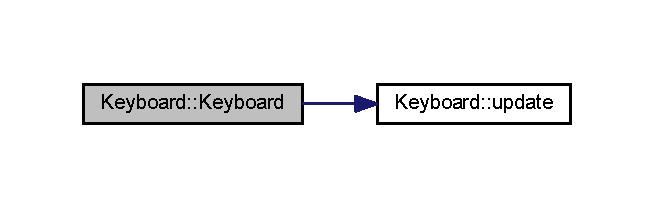
\includegraphics[width=314pt]{class_keyboard_ad6b0bb849d6bb7cdf63091e40b5f5f7f_cgraph}
\end{center}
\end{figure}




\subsection{Member Function Documentation}
\hypertarget{class_keyboard_acb69c710e18e3578fa5ed66e07e6b766}{\index{Keyboard@{Keyboard}!get\-A@{get\-A}}
\index{get\-A@{get\-A}!Keyboard@{Keyboard}}
\subsubsection[{get\-A}]{\setlength{\rightskip}{0pt plus 5cm}bool Keyboard\-::get\-A (
\begin{DoxyParamCaption}
{}
\end{DoxyParamCaption}
)\hspace{0.3cm}{\ttfamily [inline]}}}\label{class_keyboard_acb69c710e18e3578fa5ed66e07e6b766}
\hypertarget{class_keyboard_aafc539a77070e0d53551199bf69877d8}{\index{Keyboard@{Keyboard}!get\-Add@{get\-Add}}
\index{get\-Add@{get\-Add}!Keyboard@{Keyboard}}
\subsubsection[{get\-Add}]{\setlength{\rightskip}{0pt plus 5cm}bool Keyboard\-::get\-Add (
\begin{DoxyParamCaption}
{}
\end{DoxyParamCaption}
)\hspace{0.3cm}{\ttfamily [inline]}}}\label{class_keyboard_aafc539a77070e0d53551199bf69877d8}
\hypertarget{class_keyboard_abe467d1841c9c0b89c5856e9b3259980}{\index{Keyboard@{Keyboard}!get\-B@{get\-B}}
\index{get\-B@{get\-B}!Keyboard@{Keyboard}}
\subsubsection[{get\-B}]{\setlength{\rightskip}{0pt plus 5cm}bool Keyboard\-::get\-B (
\begin{DoxyParamCaption}
{}
\end{DoxyParamCaption}
)\hspace{0.3cm}{\ttfamily [inline]}}}\label{class_keyboard_abe467d1841c9c0b89c5856e9b3259980}
\hypertarget{class_keyboard_a57019e241d4e3413ee6bd68e6a6a3d79}{\index{Keyboard@{Keyboard}!get\-Back\-Slash@{get\-Back\-Slash}}
\index{get\-Back\-Slash@{get\-Back\-Slash}!Keyboard@{Keyboard}}
\subsubsection[{get\-Back\-Slash}]{\setlength{\rightskip}{0pt plus 5cm}bool Keyboard\-::get\-Back\-Slash (
\begin{DoxyParamCaption}
{}
\end{DoxyParamCaption}
)\hspace{0.3cm}{\ttfamily [inline]}}}\label{class_keyboard_a57019e241d4e3413ee6bd68e6a6a3d79}
\hypertarget{class_keyboard_ab425b0b196ffde8d878097b71884702a}{\index{Keyboard@{Keyboard}!get\-Back\-Space@{get\-Back\-Space}}
\index{get\-Back\-Space@{get\-Back\-Space}!Keyboard@{Keyboard}}
\subsubsection[{get\-Back\-Space}]{\setlength{\rightskip}{0pt plus 5cm}bool Keyboard\-::get\-Back\-Space (
\begin{DoxyParamCaption}
{}
\end{DoxyParamCaption}
)\hspace{0.3cm}{\ttfamily [inline]}}}\label{class_keyboard_ab425b0b196ffde8d878097b71884702a}
\hypertarget{class_keyboard_ae14994ae9d4a753c90511eee46f9b8eb}{\index{Keyboard@{Keyboard}!get\-C@{get\-C}}
\index{get\-C@{get\-C}!Keyboard@{Keyboard}}
\subsubsection[{get\-C}]{\setlength{\rightskip}{0pt plus 5cm}bool Keyboard\-::get\-C (
\begin{DoxyParamCaption}
{}
\end{DoxyParamCaption}
)\hspace{0.3cm}{\ttfamily [inline]}}}\label{class_keyboard_ae14994ae9d4a753c90511eee46f9b8eb}
\hypertarget{class_keyboard_aec17bf7d0b87ccdd5020ab9fa3b94413}{\index{Keyboard@{Keyboard}!get\-Comma@{get\-Comma}}
\index{get\-Comma@{get\-Comma}!Keyboard@{Keyboard}}
\subsubsection[{get\-Comma}]{\setlength{\rightskip}{0pt plus 5cm}bool Keyboard\-::get\-Comma (
\begin{DoxyParamCaption}
{}
\end{DoxyParamCaption}
)\hspace{0.3cm}{\ttfamily [inline]}}}\label{class_keyboard_aec17bf7d0b87ccdd5020ab9fa3b94413}
\hypertarget{class_keyboard_ab9e7561799ddc1941283333dcd50c5e1}{\index{Keyboard@{Keyboard}!get\-D@{get\-D}}
\index{get\-D@{get\-D}!Keyboard@{Keyboard}}
\subsubsection[{get\-D}]{\setlength{\rightskip}{0pt plus 5cm}bool Keyboard\-::get\-D (
\begin{DoxyParamCaption}
{}
\end{DoxyParamCaption}
)\hspace{0.3cm}{\ttfamily [inline]}}}\label{class_keyboard_ab9e7561799ddc1941283333dcd50c5e1}
\hypertarget{class_keyboard_a2b629ac3f7efb81b4dd6091894261900}{\index{Keyboard@{Keyboard}!get\-Dash@{get\-Dash}}
\index{get\-Dash@{get\-Dash}!Keyboard@{Keyboard}}
\subsubsection[{get\-Dash}]{\setlength{\rightskip}{0pt plus 5cm}bool Keyboard\-::get\-Dash (
\begin{DoxyParamCaption}
{}
\end{DoxyParamCaption}
)\hspace{0.3cm}{\ttfamily [inline]}}}\label{class_keyboard_a2b629ac3f7efb81b4dd6091894261900}
\hypertarget{class_keyboard_aa65d80a94c32f9a3180d4c73049165fd}{\index{Keyboard@{Keyboard}!get\-Delete@{get\-Delete}}
\index{get\-Delete@{get\-Delete}!Keyboard@{Keyboard}}
\subsubsection[{get\-Delete}]{\setlength{\rightskip}{0pt plus 5cm}bool Keyboard\-::get\-Delete (
\begin{DoxyParamCaption}
{}
\end{DoxyParamCaption}
)\hspace{0.3cm}{\ttfamily [inline]}}}\label{class_keyboard_aa65d80a94c32f9a3180d4c73049165fd}
\hypertarget{class_keyboard_abca2a6295ec794e1547ced02396b4835}{\index{Keyboard@{Keyboard}!get\-Divide@{get\-Divide}}
\index{get\-Divide@{get\-Divide}!Keyboard@{Keyboard}}
\subsubsection[{get\-Divide}]{\setlength{\rightskip}{0pt plus 5cm}bool Keyboard\-::get\-Divide (
\begin{DoxyParamCaption}
{}
\end{DoxyParamCaption}
)\hspace{0.3cm}{\ttfamily [inline]}}}\label{class_keyboard_abca2a6295ec794e1547ced02396b4835}
\hypertarget{class_keyboard_a9d07f97d9a6d654c768864fbd3beea23}{\index{Keyboard@{Keyboard}!get\-Down@{get\-Down}}
\index{get\-Down@{get\-Down}!Keyboard@{Keyboard}}
\subsubsection[{get\-Down}]{\setlength{\rightskip}{0pt plus 5cm}bool Keyboard\-::get\-Down (
\begin{DoxyParamCaption}
{}
\end{DoxyParamCaption}
)\hspace{0.3cm}{\ttfamily [inline]}}}\label{class_keyboard_a9d07f97d9a6d654c768864fbd3beea23}
\hypertarget{class_keyboard_ac1fbe5b7e31739174b7cd810521a2e9d}{\index{Keyboard@{Keyboard}!get\-E@{get\-E}}
\index{get\-E@{get\-E}!Keyboard@{Keyboard}}
\subsubsection[{get\-E}]{\setlength{\rightskip}{0pt plus 5cm}bool Keyboard\-::get\-E (
\begin{DoxyParamCaption}
{}
\end{DoxyParamCaption}
)\hspace{0.3cm}{\ttfamily [inline]}}}\label{class_keyboard_ac1fbe5b7e31739174b7cd810521a2e9d}
\hypertarget{class_keyboard_adbbf01e7ad22f2c1f1253053a90524c2}{\index{Keyboard@{Keyboard}!get\-End@{get\-End}}
\index{get\-End@{get\-End}!Keyboard@{Keyboard}}
\subsubsection[{get\-End}]{\setlength{\rightskip}{0pt plus 5cm}bool Keyboard\-::get\-End (
\begin{DoxyParamCaption}
{}
\end{DoxyParamCaption}
)\hspace{0.3cm}{\ttfamily [inline]}}}\label{class_keyboard_adbbf01e7ad22f2c1f1253053a90524c2}
\hypertarget{class_keyboard_ab33d990d565c0e9e6de234c2ccd847fd}{\index{Keyboard@{Keyboard}!get\-Equal@{get\-Equal}}
\index{get\-Equal@{get\-Equal}!Keyboard@{Keyboard}}
\subsubsection[{get\-Equal}]{\setlength{\rightskip}{0pt plus 5cm}bool Keyboard\-::get\-Equal (
\begin{DoxyParamCaption}
{}
\end{DoxyParamCaption}
)\hspace{0.3cm}{\ttfamily [inline]}}}\label{class_keyboard_ab33d990d565c0e9e6de234c2ccd847fd}
\hypertarget{class_keyboard_a994ab28476380c8233e80cb0f349bdb8}{\index{Keyboard@{Keyboard}!get\-Escape@{get\-Escape}}
\index{get\-Escape@{get\-Escape}!Keyboard@{Keyboard}}
\subsubsection[{get\-Escape}]{\setlength{\rightskip}{0pt plus 5cm}bool Keyboard\-::get\-Escape (
\begin{DoxyParamCaption}
{}
\end{DoxyParamCaption}
)\hspace{0.3cm}{\ttfamily [inline]}}}\label{class_keyboard_a994ab28476380c8233e80cb0f349bdb8}
\hypertarget{class_keyboard_a6fec87afe52371c8a264745a5c487d06}{\index{Keyboard@{Keyboard}!get\-F@{get\-F}}
\index{get\-F@{get\-F}!Keyboard@{Keyboard}}
\subsubsection[{get\-F}]{\setlength{\rightskip}{0pt plus 5cm}bool Keyboard\-::get\-F (
\begin{DoxyParamCaption}
{}
\end{DoxyParamCaption}
)\hspace{0.3cm}{\ttfamily [inline]}}}\label{class_keyboard_a6fec87afe52371c8a264745a5c487d06}
\hypertarget{class_keyboard_a89d9b338c53114a8a736b33e9767f72e}{\index{Keyboard@{Keyboard}!get\-F1@{get\-F1}}
\index{get\-F1@{get\-F1}!Keyboard@{Keyboard}}
\subsubsection[{get\-F1}]{\setlength{\rightskip}{0pt plus 5cm}bool Keyboard\-::get\-F1 (
\begin{DoxyParamCaption}
{}
\end{DoxyParamCaption}
)\hspace{0.3cm}{\ttfamily [inline]}}}\label{class_keyboard_a89d9b338c53114a8a736b33e9767f72e}
\hypertarget{class_keyboard_ae8a49362a97f0f85ed9f9d4430d3ce39}{\index{Keyboard@{Keyboard}!get\-F10@{get\-F10}}
\index{get\-F10@{get\-F10}!Keyboard@{Keyboard}}
\subsubsection[{get\-F10}]{\setlength{\rightskip}{0pt plus 5cm}bool Keyboard\-::get\-F10 (
\begin{DoxyParamCaption}
{}
\end{DoxyParamCaption}
)\hspace{0.3cm}{\ttfamily [inline]}}}\label{class_keyboard_ae8a49362a97f0f85ed9f9d4430d3ce39}
\hypertarget{class_keyboard_a88608100c5a4e694922ce5054888407e}{\index{Keyboard@{Keyboard}!get\-F11@{get\-F11}}
\index{get\-F11@{get\-F11}!Keyboard@{Keyboard}}
\subsubsection[{get\-F11}]{\setlength{\rightskip}{0pt plus 5cm}bool Keyboard\-::get\-F11 (
\begin{DoxyParamCaption}
{}
\end{DoxyParamCaption}
)\hspace{0.3cm}{\ttfamily [inline]}}}\label{class_keyboard_a88608100c5a4e694922ce5054888407e}
\hypertarget{class_keyboard_a322c334deaf0b92c93416816a482b6ba}{\index{Keyboard@{Keyboard}!get\-F12@{get\-F12}}
\index{get\-F12@{get\-F12}!Keyboard@{Keyboard}}
\subsubsection[{get\-F12}]{\setlength{\rightskip}{0pt plus 5cm}bool Keyboard\-::get\-F12 (
\begin{DoxyParamCaption}
{}
\end{DoxyParamCaption}
)\hspace{0.3cm}{\ttfamily [inline]}}}\label{class_keyboard_a322c334deaf0b92c93416816a482b6ba}
\hypertarget{class_keyboard_abff30ad0570f44cb49f979b7f88f76ea}{\index{Keyboard@{Keyboard}!get\-F13@{get\-F13}}
\index{get\-F13@{get\-F13}!Keyboard@{Keyboard}}
\subsubsection[{get\-F13}]{\setlength{\rightskip}{0pt plus 5cm}bool Keyboard\-::get\-F13 (
\begin{DoxyParamCaption}
{}
\end{DoxyParamCaption}
)\hspace{0.3cm}{\ttfamily [inline]}}}\label{class_keyboard_abff30ad0570f44cb49f979b7f88f76ea}
\hypertarget{class_keyboard_af1814f932c5b125d113c99a0879c22a0}{\index{Keyboard@{Keyboard}!get\-F14@{get\-F14}}
\index{get\-F14@{get\-F14}!Keyboard@{Keyboard}}
\subsubsection[{get\-F14}]{\setlength{\rightskip}{0pt plus 5cm}bool Keyboard\-::get\-F14 (
\begin{DoxyParamCaption}
{}
\end{DoxyParamCaption}
)\hspace{0.3cm}{\ttfamily [inline]}}}\label{class_keyboard_af1814f932c5b125d113c99a0879c22a0}
\hypertarget{class_keyboard_a2d62f212870972657e5ae965a11df89d}{\index{Keyboard@{Keyboard}!get\-F15@{get\-F15}}
\index{get\-F15@{get\-F15}!Keyboard@{Keyboard}}
\subsubsection[{get\-F15}]{\setlength{\rightskip}{0pt plus 5cm}bool Keyboard\-::get\-F15 (
\begin{DoxyParamCaption}
{}
\end{DoxyParamCaption}
)\hspace{0.3cm}{\ttfamily [inline]}}}\label{class_keyboard_a2d62f212870972657e5ae965a11df89d}
\hypertarget{class_keyboard_a2fec13e7b4db8d34fd460f178b14e54c}{\index{Keyboard@{Keyboard}!get\-F2@{get\-F2}}
\index{get\-F2@{get\-F2}!Keyboard@{Keyboard}}
\subsubsection[{get\-F2}]{\setlength{\rightskip}{0pt plus 5cm}bool Keyboard\-::get\-F2 (
\begin{DoxyParamCaption}
{}
\end{DoxyParamCaption}
)\hspace{0.3cm}{\ttfamily [inline]}}}\label{class_keyboard_a2fec13e7b4db8d34fd460f178b14e54c}
\hypertarget{class_keyboard_a82cc37753de536fed35da764e6c30d26}{\index{Keyboard@{Keyboard}!get\-F3@{get\-F3}}
\index{get\-F3@{get\-F3}!Keyboard@{Keyboard}}
\subsubsection[{get\-F3}]{\setlength{\rightskip}{0pt plus 5cm}bool Keyboard\-::get\-F3 (
\begin{DoxyParamCaption}
{}
\end{DoxyParamCaption}
)\hspace{0.3cm}{\ttfamily [inline]}}}\label{class_keyboard_a82cc37753de536fed35da764e6c30d26}
\hypertarget{class_keyboard_ac9c2d3a80291c00101e4d89661be33a8}{\index{Keyboard@{Keyboard}!get\-F4@{get\-F4}}
\index{get\-F4@{get\-F4}!Keyboard@{Keyboard}}
\subsubsection[{get\-F4}]{\setlength{\rightskip}{0pt plus 5cm}bool Keyboard\-::get\-F4 (
\begin{DoxyParamCaption}
{}
\end{DoxyParamCaption}
)\hspace{0.3cm}{\ttfamily [inline]}}}\label{class_keyboard_ac9c2d3a80291c00101e4d89661be33a8}
\hypertarget{class_keyboard_ac10076d1fe94851272cc90cf6690b8cc}{\index{Keyboard@{Keyboard}!get\-F5@{get\-F5}}
\index{get\-F5@{get\-F5}!Keyboard@{Keyboard}}
\subsubsection[{get\-F5}]{\setlength{\rightskip}{0pt plus 5cm}bool Keyboard\-::get\-F5 (
\begin{DoxyParamCaption}
{}
\end{DoxyParamCaption}
)\hspace{0.3cm}{\ttfamily [inline]}}}\label{class_keyboard_ac10076d1fe94851272cc90cf6690b8cc}
\hypertarget{class_keyboard_adc476a2af4f6ef9a983da62d8d2fed0a}{\index{Keyboard@{Keyboard}!get\-F6@{get\-F6}}
\index{get\-F6@{get\-F6}!Keyboard@{Keyboard}}
\subsubsection[{get\-F6}]{\setlength{\rightskip}{0pt plus 5cm}bool Keyboard\-::get\-F6 (
\begin{DoxyParamCaption}
{}
\end{DoxyParamCaption}
)\hspace{0.3cm}{\ttfamily [inline]}}}\label{class_keyboard_adc476a2af4f6ef9a983da62d8d2fed0a}
\hypertarget{class_keyboard_a8e843446827b1c258aaff1d5c0ad0024}{\index{Keyboard@{Keyboard}!get\-F7@{get\-F7}}
\index{get\-F7@{get\-F7}!Keyboard@{Keyboard}}
\subsubsection[{get\-F7}]{\setlength{\rightskip}{0pt plus 5cm}bool Keyboard\-::get\-F7 (
\begin{DoxyParamCaption}
{}
\end{DoxyParamCaption}
)\hspace{0.3cm}{\ttfamily [inline]}}}\label{class_keyboard_a8e843446827b1c258aaff1d5c0ad0024}
\hypertarget{class_keyboard_ae875c4c35788a819158e2c1a7628d8f6}{\index{Keyboard@{Keyboard}!get\-F8@{get\-F8}}
\index{get\-F8@{get\-F8}!Keyboard@{Keyboard}}
\subsubsection[{get\-F8}]{\setlength{\rightskip}{0pt plus 5cm}bool Keyboard\-::get\-F8 (
\begin{DoxyParamCaption}
{}
\end{DoxyParamCaption}
)\hspace{0.3cm}{\ttfamily [inline]}}}\label{class_keyboard_ae875c4c35788a819158e2c1a7628d8f6}
\hypertarget{class_keyboard_a154b39d12c6f8cc1c5bfbbb5282bc7e3}{\index{Keyboard@{Keyboard}!get\-F9@{get\-F9}}
\index{get\-F9@{get\-F9}!Keyboard@{Keyboard}}
\subsubsection[{get\-F9}]{\setlength{\rightskip}{0pt plus 5cm}bool Keyboard\-::get\-F9 (
\begin{DoxyParamCaption}
{}
\end{DoxyParamCaption}
)\hspace{0.3cm}{\ttfamily [inline]}}}\label{class_keyboard_a154b39d12c6f8cc1c5bfbbb5282bc7e3}
\hypertarget{class_keyboard_a31aae98dfbc61407fa004ae2f7595452}{\index{Keyboard@{Keyboard}!get\-G@{get\-G}}
\index{get\-G@{get\-G}!Keyboard@{Keyboard}}
\subsubsection[{get\-G}]{\setlength{\rightskip}{0pt plus 5cm}bool Keyboard\-::get\-G (
\begin{DoxyParamCaption}
{}
\end{DoxyParamCaption}
)\hspace{0.3cm}{\ttfamily [inline]}}}\label{class_keyboard_a31aae98dfbc61407fa004ae2f7595452}
\hypertarget{class_keyboard_a0deba682104bf09a85d23ab4085d53f8}{\index{Keyboard@{Keyboard}!get\-H@{get\-H}}
\index{get\-H@{get\-H}!Keyboard@{Keyboard}}
\subsubsection[{get\-H}]{\setlength{\rightskip}{0pt plus 5cm}bool Keyboard\-::get\-H (
\begin{DoxyParamCaption}
{}
\end{DoxyParamCaption}
)\hspace{0.3cm}{\ttfamily [inline]}}}\label{class_keyboard_a0deba682104bf09a85d23ab4085d53f8}
\hypertarget{class_keyboard_aaa8d566aa66eddbe2a3a3ce5565cb34f}{\index{Keyboard@{Keyboard}!get\-Home@{get\-Home}}
\index{get\-Home@{get\-Home}!Keyboard@{Keyboard}}
\subsubsection[{get\-Home}]{\setlength{\rightskip}{0pt plus 5cm}bool Keyboard\-::get\-Home (
\begin{DoxyParamCaption}
{}
\end{DoxyParamCaption}
)\hspace{0.3cm}{\ttfamily [inline]}}}\label{class_keyboard_aaa8d566aa66eddbe2a3a3ce5565cb34f}
\hypertarget{class_keyboard_a533b9c9ea72e078a6ed1081e0293a457}{\index{Keyboard@{Keyboard}!get\-I@{get\-I}}
\index{get\-I@{get\-I}!Keyboard@{Keyboard}}
\subsubsection[{get\-I}]{\setlength{\rightskip}{0pt plus 5cm}bool Keyboard\-::get\-I (
\begin{DoxyParamCaption}
{}
\end{DoxyParamCaption}
)\hspace{0.3cm}{\ttfamily [inline]}}}\label{class_keyboard_a533b9c9ea72e078a6ed1081e0293a457}
\hypertarget{class_keyboard_a78814c54bdbb71866480a73bec46c1da}{\index{Keyboard@{Keyboard}!get\-Insert@{get\-Insert}}
\index{get\-Insert@{get\-Insert}!Keyboard@{Keyboard}}
\subsubsection[{get\-Insert}]{\setlength{\rightskip}{0pt plus 5cm}bool Keyboard\-::get\-Insert (
\begin{DoxyParamCaption}
{}
\end{DoxyParamCaption}
)\hspace{0.3cm}{\ttfamily [inline]}}}\label{class_keyboard_a78814c54bdbb71866480a73bec46c1da}
\hypertarget{class_keyboard_a09fc76a431abc21dba175b10bc4a1ec8}{\index{Keyboard@{Keyboard}!get\-Instance@{get\-Instance}}
\index{get\-Instance@{get\-Instance}!Keyboard@{Keyboard}}
\subsubsection[{get\-Instance}]{\setlength{\rightskip}{0pt plus 5cm}{\bf Keyboard} \& Keyboard\-::get\-Instance (
\begin{DoxyParamCaption}
{}
\end{DoxyParamCaption}
)\hspace{0.3cm}{\ttfamily [static]}}}\label{class_keyboard_a09fc76a431abc21dba175b10bc4a1ec8}


Here is the caller graph for this function\-:\nopagebreak
\begin{figure}[H]
\begin{center}
\leavevmode
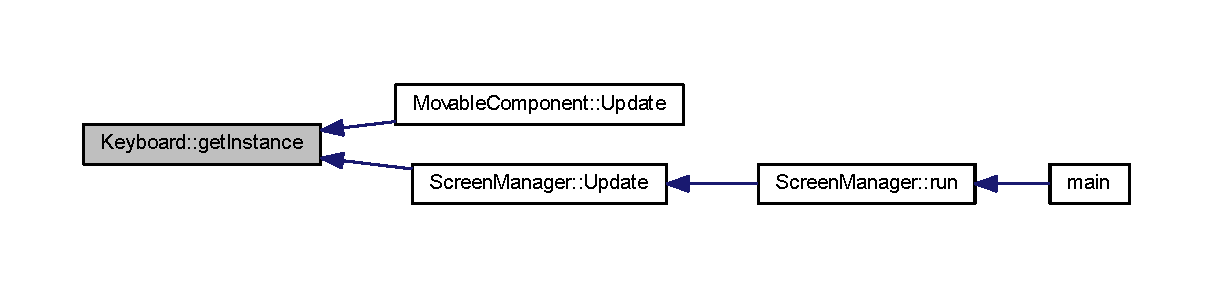
\includegraphics[width=350pt]{class_keyboard_a09fc76a431abc21dba175b10bc4a1ec8_icgraph}
\end{center}
\end{figure}


\hypertarget{class_keyboard_a47d68d720a385e1b58d28ecffbf97964}{\index{Keyboard@{Keyboard}!get\-J@{get\-J}}
\index{get\-J@{get\-J}!Keyboard@{Keyboard}}
\subsubsection[{get\-J}]{\setlength{\rightskip}{0pt plus 5cm}bool Keyboard\-::get\-J (
\begin{DoxyParamCaption}
{}
\end{DoxyParamCaption}
)\hspace{0.3cm}{\ttfamily [inline]}}}\label{class_keyboard_a47d68d720a385e1b58d28ecffbf97964}
\hypertarget{class_keyboard_ac512b5cbd9f8c229a6a4c81c0ca12f91}{\index{Keyboard@{Keyboard}!get\-K@{get\-K}}
\index{get\-K@{get\-K}!Keyboard@{Keyboard}}
\subsubsection[{get\-K}]{\setlength{\rightskip}{0pt plus 5cm}bool Keyboard\-::get\-K (
\begin{DoxyParamCaption}
{}
\end{DoxyParamCaption}
)\hspace{0.3cm}{\ttfamily [inline]}}}\label{class_keyboard_ac512b5cbd9f8c229a6a4c81c0ca12f91}
\hypertarget{class_keyboard_a0bb30d06c8ed37ae9e0e55135f2b7170}{\index{Keyboard@{Keyboard}!get\-L@{get\-L}}
\index{get\-L@{get\-L}!Keyboard@{Keyboard}}
\subsubsection[{get\-L}]{\setlength{\rightskip}{0pt plus 5cm}bool Keyboard\-::get\-L (
\begin{DoxyParamCaption}
{}
\end{DoxyParamCaption}
)\hspace{0.3cm}{\ttfamily [inline]}}}\label{class_keyboard_a0bb30d06c8ed37ae9e0e55135f2b7170}
\hypertarget{class_keyboard_a2ad4b6abd18ebd2a6c69da2de338265c}{\index{Keyboard@{Keyboard}!get\-L\-Alt@{get\-L\-Alt}}
\index{get\-L\-Alt@{get\-L\-Alt}!Keyboard@{Keyboard}}
\subsubsection[{get\-L\-Alt}]{\setlength{\rightskip}{0pt plus 5cm}bool Keyboard\-::get\-L\-Alt (
\begin{DoxyParamCaption}
{}
\end{DoxyParamCaption}
)\hspace{0.3cm}{\ttfamily [inline]}}}\label{class_keyboard_a2ad4b6abd18ebd2a6c69da2de338265c}
\hypertarget{class_keyboard_a62d0bd6e13a7c2ef5d70f0c63c7b6104}{\index{Keyboard@{Keyboard}!get\-L\-Bracket@{get\-L\-Bracket}}
\index{get\-L\-Bracket@{get\-L\-Bracket}!Keyboard@{Keyboard}}
\subsubsection[{get\-L\-Bracket}]{\setlength{\rightskip}{0pt plus 5cm}bool Keyboard\-::get\-L\-Bracket (
\begin{DoxyParamCaption}
{}
\end{DoxyParamCaption}
)\hspace{0.3cm}{\ttfamily [inline]}}}\label{class_keyboard_a62d0bd6e13a7c2ef5d70f0c63c7b6104}
\hypertarget{class_keyboard_a5f60b99ed9f012e78629acfe1f795be3}{\index{Keyboard@{Keyboard}!get\-L\-Control@{get\-L\-Control}}
\index{get\-L\-Control@{get\-L\-Control}!Keyboard@{Keyboard}}
\subsubsection[{get\-L\-Control}]{\setlength{\rightskip}{0pt plus 5cm}bool Keyboard\-::get\-L\-Control (
\begin{DoxyParamCaption}
{}
\end{DoxyParamCaption}
)\hspace{0.3cm}{\ttfamily [inline]}}}\label{class_keyboard_a5f60b99ed9f012e78629acfe1f795be3}
\hypertarget{class_keyboard_ac8b072ea0e90e87b10470bc92cec1a5c}{\index{Keyboard@{Keyboard}!get\-Left@{get\-Left}}
\index{get\-Left@{get\-Left}!Keyboard@{Keyboard}}
\subsubsection[{get\-Left}]{\setlength{\rightskip}{0pt plus 5cm}bool Keyboard\-::get\-Left (
\begin{DoxyParamCaption}
{}
\end{DoxyParamCaption}
)\hspace{0.3cm}{\ttfamily [inline]}}}\label{class_keyboard_ac8b072ea0e90e87b10470bc92cec1a5c}
\hypertarget{class_keyboard_a410f25adf92d4120faeab8334ededba9}{\index{Keyboard@{Keyboard}!get\-L\-Shift@{get\-L\-Shift}}
\index{get\-L\-Shift@{get\-L\-Shift}!Keyboard@{Keyboard}}
\subsubsection[{get\-L\-Shift}]{\setlength{\rightskip}{0pt plus 5cm}bool Keyboard\-::get\-L\-Shift (
\begin{DoxyParamCaption}
{}
\end{DoxyParamCaption}
)\hspace{0.3cm}{\ttfamily [inline]}}}\label{class_keyboard_a410f25adf92d4120faeab8334ededba9}
\hypertarget{class_keyboard_ab58d4d9bb82bf64de46fa1792fd80086}{\index{Keyboard@{Keyboard}!get\-L\-System@{get\-L\-System}}
\index{get\-L\-System@{get\-L\-System}!Keyboard@{Keyboard}}
\subsubsection[{get\-L\-System}]{\setlength{\rightskip}{0pt plus 5cm}bool Keyboard\-::get\-L\-System (
\begin{DoxyParamCaption}
{}
\end{DoxyParamCaption}
)\hspace{0.3cm}{\ttfamily [inline]}}}\label{class_keyboard_ab58d4d9bb82bf64de46fa1792fd80086}
\hypertarget{class_keyboard_a06888fa46c0dc92103a4d7416bfb474e}{\index{Keyboard@{Keyboard}!get\-M@{get\-M}}
\index{get\-M@{get\-M}!Keyboard@{Keyboard}}
\subsubsection[{get\-M}]{\setlength{\rightskip}{0pt plus 5cm}bool Keyboard\-::get\-M (
\begin{DoxyParamCaption}
{}
\end{DoxyParamCaption}
)\hspace{0.3cm}{\ttfamily [inline]}}}\label{class_keyboard_a06888fa46c0dc92103a4d7416bfb474e}
\hypertarget{class_keyboard_ad5c31b46ab392c8cfeb4f060ce346e22}{\index{Keyboard@{Keyboard}!get\-Menu@{get\-Menu}}
\index{get\-Menu@{get\-Menu}!Keyboard@{Keyboard}}
\subsubsection[{get\-Menu}]{\setlength{\rightskip}{0pt plus 5cm}bool Keyboard\-::get\-Menu (
\begin{DoxyParamCaption}
{}
\end{DoxyParamCaption}
)\hspace{0.3cm}{\ttfamily [inline]}}}\label{class_keyboard_ad5c31b46ab392c8cfeb4f060ce346e22}
\hypertarget{class_keyboard_a9971de37c9040738efa45a0e51aee175}{\index{Keyboard@{Keyboard}!get\-Multiply@{get\-Multiply}}
\index{get\-Multiply@{get\-Multiply}!Keyboard@{Keyboard}}
\subsubsection[{get\-Multiply}]{\setlength{\rightskip}{0pt plus 5cm}bool Keyboard\-::get\-Multiply (
\begin{DoxyParamCaption}
{}
\end{DoxyParamCaption}
)\hspace{0.3cm}{\ttfamily [inline]}}}\label{class_keyboard_a9971de37c9040738efa45a0e51aee175}
\hypertarget{class_keyboard_a0b5d31dc62328f59af7ff137de090818}{\index{Keyboard@{Keyboard}!get\-N@{get\-N}}
\index{get\-N@{get\-N}!Keyboard@{Keyboard}}
\subsubsection[{get\-N}]{\setlength{\rightskip}{0pt plus 5cm}bool Keyboard\-::get\-N (
\begin{DoxyParamCaption}
{}
\end{DoxyParamCaption}
)\hspace{0.3cm}{\ttfamily [inline]}}}\label{class_keyboard_a0b5d31dc62328f59af7ff137de090818}
\hypertarget{class_keyboard_a1c5ecb4909477ec4a5173353171912bd}{\index{Keyboard@{Keyboard}!get\-Num0@{get\-Num0}}
\index{get\-Num0@{get\-Num0}!Keyboard@{Keyboard}}
\subsubsection[{get\-Num0}]{\setlength{\rightskip}{0pt plus 5cm}bool Keyboard\-::get\-Num0 (
\begin{DoxyParamCaption}
{}
\end{DoxyParamCaption}
)\hspace{0.3cm}{\ttfamily [inline]}}}\label{class_keyboard_a1c5ecb4909477ec4a5173353171912bd}
\hypertarget{class_keyboard_a27d7ebfb0172d399530245cd00243fb0}{\index{Keyboard@{Keyboard}!get\-Num1@{get\-Num1}}
\index{get\-Num1@{get\-Num1}!Keyboard@{Keyboard}}
\subsubsection[{get\-Num1}]{\setlength{\rightskip}{0pt plus 5cm}bool Keyboard\-::get\-Num1 (
\begin{DoxyParamCaption}
{}
\end{DoxyParamCaption}
)\hspace{0.3cm}{\ttfamily [inline]}}}\label{class_keyboard_a27d7ebfb0172d399530245cd00243fb0}
\hypertarget{class_keyboard_a6e5e05e63ae1cfb59ca375b05dcbe688}{\index{Keyboard@{Keyboard}!get\-Num2@{get\-Num2}}
\index{get\-Num2@{get\-Num2}!Keyboard@{Keyboard}}
\subsubsection[{get\-Num2}]{\setlength{\rightskip}{0pt plus 5cm}bool Keyboard\-::get\-Num2 (
\begin{DoxyParamCaption}
{}
\end{DoxyParamCaption}
)\hspace{0.3cm}{\ttfamily [inline]}}}\label{class_keyboard_a6e5e05e63ae1cfb59ca375b05dcbe688}
\hypertarget{class_keyboard_acb62d27041dd2d39968c2d2fe424155d}{\index{Keyboard@{Keyboard}!get\-Num3@{get\-Num3}}
\index{get\-Num3@{get\-Num3}!Keyboard@{Keyboard}}
\subsubsection[{get\-Num3}]{\setlength{\rightskip}{0pt plus 5cm}bool Keyboard\-::get\-Num3 (
\begin{DoxyParamCaption}
{}
\end{DoxyParamCaption}
)\hspace{0.3cm}{\ttfamily [inline]}}}\label{class_keyboard_acb62d27041dd2d39968c2d2fe424155d}
\hypertarget{class_keyboard_adf405bac73bbe34b554b452ce531fd09}{\index{Keyboard@{Keyboard}!get\-Num4@{get\-Num4}}
\index{get\-Num4@{get\-Num4}!Keyboard@{Keyboard}}
\subsubsection[{get\-Num4}]{\setlength{\rightskip}{0pt plus 5cm}bool Keyboard\-::get\-Num4 (
\begin{DoxyParamCaption}
{}
\end{DoxyParamCaption}
)\hspace{0.3cm}{\ttfamily [inline]}}}\label{class_keyboard_adf405bac73bbe34b554b452ce531fd09}
\hypertarget{class_keyboard_a5a172c6bab05bb95d20ddb80a2d23d95}{\index{Keyboard@{Keyboard}!get\-Num5@{get\-Num5}}
\index{get\-Num5@{get\-Num5}!Keyboard@{Keyboard}}
\subsubsection[{get\-Num5}]{\setlength{\rightskip}{0pt plus 5cm}bool Keyboard\-::get\-Num5 (
\begin{DoxyParamCaption}
{}
\end{DoxyParamCaption}
)\hspace{0.3cm}{\ttfamily [inline]}}}\label{class_keyboard_a5a172c6bab05bb95d20ddb80a2d23d95}
\hypertarget{class_keyboard_af08887ae78e829222420acada6707ac8}{\index{Keyboard@{Keyboard}!get\-Num6@{get\-Num6}}
\index{get\-Num6@{get\-Num6}!Keyboard@{Keyboard}}
\subsubsection[{get\-Num6}]{\setlength{\rightskip}{0pt plus 5cm}bool Keyboard\-::get\-Num6 (
\begin{DoxyParamCaption}
{}
\end{DoxyParamCaption}
)\hspace{0.3cm}{\ttfamily [inline]}}}\label{class_keyboard_af08887ae78e829222420acada6707ac8}
\hypertarget{class_keyboard_a08d1067ac6b0c8836f01608e60842625}{\index{Keyboard@{Keyboard}!get\-Num7@{get\-Num7}}
\index{get\-Num7@{get\-Num7}!Keyboard@{Keyboard}}
\subsubsection[{get\-Num7}]{\setlength{\rightskip}{0pt plus 5cm}bool Keyboard\-::get\-Num7 (
\begin{DoxyParamCaption}
{}
\end{DoxyParamCaption}
)\hspace{0.3cm}{\ttfamily [inline]}}}\label{class_keyboard_a08d1067ac6b0c8836f01608e60842625}
\hypertarget{class_keyboard_af0e119a74e4fcca0bbda53d885bd4245}{\index{Keyboard@{Keyboard}!get\-Num8@{get\-Num8}}
\index{get\-Num8@{get\-Num8}!Keyboard@{Keyboard}}
\subsubsection[{get\-Num8}]{\setlength{\rightskip}{0pt plus 5cm}bool Keyboard\-::get\-Num8 (
\begin{DoxyParamCaption}
{}
\end{DoxyParamCaption}
)\hspace{0.3cm}{\ttfamily [inline]}}}\label{class_keyboard_af0e119a74e4fcca0bbda53d885bd4245}
\hypertarget{class_keyboard_a0e1c476a2d5e4c9c0f9a7a2c97356bfa}{\index{Keyboard@{Keyboard}!get\-Num9@{get\-Num9}}
\index{get\-Num9@{get\-Num9}!Keyboard@{Keyboard}}
\subsubsection[{get\-Num9}]{\setlength{\rightskip}{0pt plus 5cm}bool Keyboard\-::get\-Num9 (
\begin{DoxyParamCaption}
{}
\end{DoxyParamCaption}
)\hspace{0.3cm}{\ttfamily [inline]}}}\label{class_keyboard_a0e1c476a2d5e4c9c0f9a7a2c97356bfa}
\hypertarget{class_keyboard_a909c70a8e72b75c9515441651b88372d}{\index{Keyboard@{Keyboard}!get\-Numpad0@{get\-Numpad0}}
\index{get\-Numpad0@{get\-Numpad0}!Keyboard@{Keyboard}}
\subsubsection[{get\-Numpad0}]{\setlength{\rightskip}{0pt plus 5cm}bool Keyboard\-::get\-Numpad0 (
\begin{DoxyParamCaption}
{}
\end{DoxyParamCaption}
)\hspace{0.3cm}{\ttfamily [inline]}}}\label{class_keyboard_a909c70a8e72b75c9515441651b88372d}
\hypertarget{class_keyboard_a1ea935eecc5f69b46898529d6e019d27}{\index{Keyboard@{Keyboard}!get\-Numpad1@{get\-Numpad1}}
\index{get\-Numpad1@{get\-Numpad1}!Keyboard@{Keyboard}}
\subsubsection[{get\-Numpad1}]{\setlength{\rightskip}{0pt plus 5cm}bool Keyboard\-::get\-Numpad1 (
\begin{DoxyParamCaption}
{}
\end{DoxyParamCaption}
)\hspace{0.3cm}{\ttfamily [inline]}}}\label{class_keyboard_a1ea935eecc5f69b46898529d6e019d27}
\hypertarget{class_keyboard_a395b15a9fa1916d79bf5fc84f87f0919}{\index{Keyboard@{Keyboard}!get\-Numpad2@{get\-Numpad2}}
\index{get\-Numpad2@{get\-Numpad2}!Keyboard@{Keyboard}}
\subsubsection[{get\-Numpad2}]{\setlength{\rightskip}{0pt plus 5cm}bool Keyboard\-::get\-Numpad2 (
\begin{DoxyParamCaption}
{}
\end{DoxyParamCaption}
)\hspace{0.3cm}{\ttfamily [inline]}}}\label{class_keyboard_a395b15a9fa1916d79bf5fc84f87f0919}
\hypertarget{class_keyboard_a650ce67f4890d668e58f8f2c459f345f}{\index{Keyboard@{Keyboard}!get\-Numpad3@{get\-Numpad3}}
\index{get\-Numpad3@{get\-Numpad3}!Keyboard@{Keyboard}}
\subsubsection[{get\-Numpad3}]{\setlength{\rightskip}{0pt plus 5cm}bool Keyboard\-::get\-Numpad3 (
\begin{DoxyParamCaption}
{}
\end{DoxyParamCaption}
)\hspace{0.3cm}{\ttfamily [inline]}}}\label{class_keyboard_a650ce67f4890d668e58f8f2c459f345f}
\hypertarget{class_keyboard_a3d9b7aa434579001274e29919da7351c}{\index{Keyboard@{Keyboard}!get\-Numpad4@{get\-Numpad4}}
\index{get\-Numpad4@{get\-Numpad4}!Keyboard@{Keyboard}}
\subsubsection[{get\-Numpad4}]{\setlength{\rightskip}{0pt plus 5cm}bool Keyboard\-::get\-Numpad4 (
\begin{DoxyParamCaption}
{}
\end{DoxyParamCaption}
)\hspace{0.3cm}{\ttfamily [inline]}}}\label{class_keyboard_a3d9b7aa434579001274e29919da7351c}
\hypertarget{class_keyboard_a39972d7e2eab16ac5af74a5ba6c0d7a2}{\index{Keyboard@{Keyboard}!get\-Numpad5@{get\-Numpad5}}
\index{get\-Numpad5@{get\-Numpad5}!Keyboard@{Keyboard}}
\subsubsection[{get\-Numpad5}]{\setlength{\rightskip}{0pt plus 5cm}bool Keyboard\-::get\-Numpad5 (
\begin{DoxyParamCaption}
{}
\end{DoxyParamCaption}
)\hspace{0.3cm}{\ttfamily [inline]}}}\label{class_keyboard_a39972d7e2eab16ac5af74a5ba6c0d7a2}
\hypertarget{class_keyboard_a72f11330e522fd2d8d6d096f703b717b}{\index{Keyboard@{Keyboard}!get\-Numpad6@{get\-Numpad6}}
\index{get\-Numpad6@{get\-Numpad6}!Keyboard@{Keyboard}}
\subsubsection[{get\-Numpad6}]{\setlength{\rightskip}{0pt plus 5cm}bool Keyboard\-::get\-Numpad6 (
\begin{DoxyParamCaption}
{}
\end{DoxyParamCaption}
)\hspace{0.3cm}{\ttfamily [inline]}}}\label{class_keyboard_a72f11330e522fd2d8d6d096f703b717b}
\hypertarget{class_keyboard_a24ebd525127b9d17386a1e6267905ef5}{\index{Keyboard@{Keyboard}!get\-Numpad7@{get\-Numpad7}}
\index{get\-Numpad7@{get\-Numpad7}!Keyboard@{Keyboard}}
\subsubsection[{get\-Numpad7}]{\setlength{\rightskip}{0pt plus 5cm}bool Keyboard\-::get\-Numpad7 (
\begin{DoxyParamCaption}
{}
\end{DoxyParamCaption}
)\hspace{0.3cm}{\ttfamily [inline]}}}\label{class_keyboard_a24ebd525127b9d17386a1e6267905ef5}
\hypertarget{class_keyboard_a181042ca4d186805ff9f3a6d36b14f1b}{\index{Keyboard@{Keyboard}!get\-Numpad8@{get\-Numpad8}}
\index{get\-Numpad8@{get\-Numpad8}!Keyboard@{Keyboard}}
\subsubsection[{get\-Numpad8}]{\setlength{\rightskip}{0pt plus 5cm}bool Keyboard\-::get\-Numpad8 (
\begin{DoxyParamCaption}
{}
\end{DoxyParamCaption}
)\hspace{0.3cm}{\ttfamily [inline]}}}\label{class_keyboard_a181042ca4d186805ff9f3a6d36b14f1b}
\hypertarget{class_keyboard_a1dcfce958bfb7957b1d6b85706f9728f}{\index{Keyboard@{Keyboard}!get\-Numpad9@{get\-Numpad9}}
\index{get\-Numpad9@{get\-Numpad9}!Keyboard@{Keyboard}}
\subsubsection[{get\-Numpad9}]{\setlength{\rightskip}{0pt plus 5cm}bool Keyboard\-::get\-Numpad9 (
\begin{DoxyParamCaption}
{}
\end{DoxyParamCaption}
)\hspace{0.3cm}{\ttfamily [inline]}}}\label{class_keyboard_a1dcfce958bfb7957b1d6b85706f9728f}
\hypertarget{class_keyboard_a1d52718b43926378944d3ec1ab4ef245}{\index{Keyboard@{Keyboard}!get\-O@{get\-O}}
\index{get\-O@{get\-O}!Keyboard@{Keyboard}}
\subsubsection[{get\-O}]{\setlength{\rightskip}{0pt plus 5cm}bool Keyboard\-::get\-O (
\begin{DoxyParamCaption}
{}
\end{DoxyParamCaption}
)\hspace{0.3cm}{\ttfamily [inline]}}}\label{class_keyboard_a1d52718b43926378944d3ec1ab4ef245}
\hypertarget{class_keyboard_a9c96638ce77e4a6bfee3f7c18bcb9b63}{\index{Keyboard@{Keyboard}!get\-P@{get\-P}}
\index{get\-P@{get\-P}!Keyboard@{Keyboard}}
\subsubsection[{get\-P}]{\setlength{\rightskip}{0pt plus 5cm}bool Keyboard\-::get\-P (
\begin{DoxyParamCaption}
{}
\end{DoxyParamCaption}
)\hspace{0.3cm}{\ttfamily [inline]}}}\label{class_keyboard_a9c96638ce77e4a6bfee3f7c18bcb9b63}
\hypertarget{class_keyboard_ac2a759e6f55eb9faf0fe483df06f0adb}{\index{Keyboard@{Keyboard}!get\-Page\-Down@{get\-Page\-Down}}
\index{get\-Page\-Down@{get\-Page\-Down}!Keyboard@{Keyboard}}
\subsubsection[{get\-Page\-Down}]{\setlength{\rightskip}{0pt plus 5cm}bool Keyboard\-::get\-Page\-Down (
\begin{DoxyParamCaption}
{}
\end{DoxyParamCaption}
)\hspace{0.3cm}{\ttfamily [inline]}}}\label{class_keyboard_ac2a759e6f55eb9faf0fe483df06f0adb}
\hypertarget{class_keyboard_a6da15fa7a8b213e66c97b32411bd8c5a}{\index{Keyboard@{Keyboard}!get\-Page\-Up@{get\-Page\-Up}}
\index{get\-Page\-Up@{get\-Page\-Up}!Keyboard@{Keyboard}}
\subsubsection[{get\-Page\-Up}]{\setlength{\rightskip}{0pt plus 5cm}bool Keyboard\-::get\-Page\-Up (
\begin{DoxyParamCaption}
{}
\end{DoxyParamCaption}
)\hspace{0.3cm}{\ttfamily [inline]}}}\label{class_keyboard_a6da15fa7a8b213e66c97b32411bd8c5a}
\hypertarget{class_keyboard_a1bf2789c0743f4f00cb5778d62242315}{\index{Keyboard@{Keyboard}!get\-Pause@{get\-Pause}}
\index{get\-Pause@{get\-Pause}!Keyboard@{Keyboard}}
\subsubsection[{get\-Pause}]{\setlength{\rightskip}{0pt plus 5cm}bool Keyboard\-::get\-Pause (
\begin{DoxyParamCaption}
{}
\end{DoxyParamCaption}
)\hspace{0.3cm}{\ttfamily [inline]}}}\label{class_keyboard_a1bf2789c0743f4f00cb5778d62242315}
\hypertarget{class_keyboard_a6fc2692d8e1006b086a82678aabdbad3}{\index{Keyboard@{Keyboard}!get\-Period@{get\-Period}}
\index{get\-Period@{get\-Period}!Keyboard@{Keyboard}}
\subsubsection[{get\-Period}]{\setlength{\rightskip}{0pt plus 5cm}bool Keyboard\-::get\-Period (
\begin{DoxyParamCaption}
{}
\end{DoxyParamCaption}
)\hspace{0.3cm}{\ttfamily [inline]}}}\label{class_keyboard_a6fc2692d8e1006b086a82678aabdbad3}
\hypertarget{class_keyboard_ad3960e897150ae3121301bff4381e56a}{\index{Keyboard@{Keyboard}!get\-Q@{get\-Q}}
\index{get\-Q@{get\-Q}!Keyboard@{Keyboard}}
\subsubsection[{get\-Q}]{\setlength{\rightskip}{0pt plus 5cm}bool Keyboard\-::get\-Q (
\begin{DoxyParamCaption}
{}
\end{DoxyParamCaption}
)\hspace{0.3cm}{\ttfamily [inline]}}}\label{class_keyboard_ad3960e897150ae3121301bff4381e56a}
\hypertarget{class_keyboard_a09b58b89fb75696031d097278eac0ec7}{\index{Keyboard@{Keyboard}!get\-Quote@{get\-Quote}}
\index{get\-Quote@{get\-Quote}!Keyboard@{Keyboard}}
\subsubsection[{get\-Quote}]{\setlength{\rightskip}{0pt plus 5cm}bool Keyboard\-::get\-Quote (
\begin{DoxyParamCaption}
{}
\end{DoxyParamCaption}
)\hspace{0.3cm}{\ttfamily [inline]}}}\label{class_keyboard_a09b58b89fb75696031d097278eac0ec7}
\hypertarget{class_keyboard_a42d4db82a7ea40418c831a8d68719ca6}{\index{Keyboard@{Keyboard}!get\-R@{get\-R}}
\index{get\-R@{get\-R}!Keyboard@{Keyboard}}
\subsubsection[{get\-R}]{\setlength{\rightskip}{0pt plus 5cm}bool Keyboard\-::get\-R (
\begin{DoxyParamCaption}
{}
\end{DoxyParamCaption}
)\hspace{0.3cm}{\ttfamily [inline]}}}\label{class_keyboard_a42d4db82a7ea40418c831a8d68719ca6}
\hypertarget{class_keyboard_a670aae3f40bf02f26fb966f25ff06234}{\index{Keyboard@{Keyboard}!get\-R\-Alt@{get\-R\-Alt}}
\index{get\-R\-Alt@{get\-R\-Alt}!Keyboard@{Keyboard}}
\subsubsection[{get\-R\-Alt}]{\setlength{\rightskip}{0pt plus 5cm}bool Keyboard\-::get\-R\-Alt (
\begin{DoxyParamCaption}
{}
\end{DoxyParamCaption}
)\hspace{0.3cm}{\ttfamily [inline]}}}\label{class_keyboard_a670aae3f40bf02f26fb966f25ff06234}
\hypertarget{class_keyboard_a065e43a5ece4a6a8790e3f8a8817ea23}{\index{Keyboard@{Keyboard}!get\-R\-Bracket@{get\-R\-Bracket}}
\index{get\-R\-Bracket@{get\-R\-Bracket}!Keyboard@{Keyboard}}
\subsubsection[{get\-R\-Bracket}]{\setlength{\rightskip}{0pt plus 5cm}bool Keyboard\-::get\-R\-Bracket (
\begin{DoxyParamCaption}
{}
\end{DoxyParamCaption}
)\hspace{0.3cm}{\ttfamily [inline]}}}\label{class_keyboard_a065e43a5ece4a6a8790e3f8a8817ea23}
\hypertarget{class_keyboard_a428d96963222eff1fefb15198403c14c}{\index{Keyboard@{Keyboard}!get\-R\-Control@{get\-R\-Control}}
\index{get\-R\-Control@{get\-R\-Control}!Keyboard@{Keyboard}}
\subsubsection[{get\-R\-Control}]{\setlength{\rightskip}{0pt plus 5cm}bool Keyboard\-::get\-R\-Control (
\begin{DoxyParamCaption}
{}
\end{DoxyParamCaption}
)\hspace{0.3cm}{\ttfamily [inline]}}}\label{class_keyboard_a428d96963222eff1fefb15198403c14c}
\hypertarget{class_keyboard_a04482f34bbd2f5d2463acbe07e8b2e56}{\index{Keyboard@{Keyboard}!get\-Return@{get\-Return}}
\index{get\-Return@{get\-Return}!Keyboard@{Keyboard}}
\subsubsection[{get\-Return}]{\setlength{\rightskip}{0pt plus 5cm}bool Keyboard\-::get\-Return (
\begin{DoxyParamCaption}
{}
\end{DoxyParamCaption}
)\hspace{0.3cm}{\ttfamily [inline]}}}\label{class_keyboard_a04482f34bbd2f5d2463acbe07e8b2e56}
\hypertarget{class_keyboard_a33607f70dec11df2ea88dfe7e49d40ef}{\index{Keyboard@{Keyboard}!get\-Right@{get\-Right}}
\index{get\-Right@{get\-Right}!Keyboard@{Keyboard}}
\subsubsection[{get\-Right}]{\setlength{\rightskip}{0pt plus 5cm}bool Keyboard\-::get\-Right (
\begin{DoxyParamCaption}
{}
\end{DoxyParamCaption}
)\hspace{0.3cm}{\ttfamily [inline]}}}\label{class_keyboard_a33607f70dec11df2ea88dfe7e49d40ef}
\hypertarget{class_keyboard_a412703b9a1957036c6ef559e804aed91}{\index{Keyboard@{Keyboard}!get\-R\-Shift@{get\-R\-Shift}}
\index{get\-R\-Shift@{get\-R\-Shift}!Keyboard@{Keyboard}}
\subsubsection[{get\-R\-Shift}]{\setlength{\rightskip}{0pt plus 5cm}bool Keyboard\-::get\-R\-Shift (
\begin{DoxyParamCaption}
{}
\end{DoxyParamCaption}
)\hspace{0.3cm}{\ttfamily [inline]}}}\label{class_keyboard_a412703b9a1957036c6ef559e804aed91}
\hypertarget{class_keyboard_a8659cc000033848acae7c18683886a92}{\index{Keyboard@{Keyboard}!get\-R\-System@{get\-R\-System}}
\index{get\-R\-System@{get\-R\-System}!Keyboard@{Keyboard}}
\subsubsection[{get\-R\-System}]{\setlength{\rightskip}{0pt plus 5cm}bool Keyboard\-::get\-R\-System (
\begin{DoxyParamCaption}
{}
\end{DoxyParamCaption}
)\hspace{0.3cm}{\ttfamily [inline]}}}\label{class_keyboard_a8659cc000033848acae7c18683886a92}
\hypertarget{class_keyboard_a38c76aa89c02ba8a98b81299278f813c}{\index{Keyboard@{Keyboard}!get\-S@{get\-S}}
\index{get\-S@{get\-S}!Keyboard@{Keyboard}}
\subsubsection[{get\-S}]{\setlength{\rightskip}{0pt plus 5cm}bool Keyboard\-::get\-S (
\begin{DoxyParamCaption}
{}
\end{DoxyParamCaption}
)\hspace{0.3cm}{\ttfamily [inline]}}}\label{class_keyboard_a38c76aa89c02ba8a98b81299278f813c}
\hypertarget{class_keyboard_add5ee27f0c650e722f0c6666ed57b022}{\index{Keyboard@{Keyboard}!get\-Semi\-Colon@{get\-Semi\-Colon}}
\index{get\-Semi\-Colon@{get\-Semi\-Colon}!Keyboard@{Keyboard}}
\subsubsection[{get\-Semi\-Colon}]{\setlength{\rightskip}{0pt plus 5cm}bool Keyboard\-::get\-Semi\-Colon (
\begin{DoxyParamCaption}
{}
\end{DoxyParamCaption}
)\hspace{0.3cm}{\ttfamily [inline]}}}\label{class_keyboard_add5ee27f0c650e722f0c6666ed57b022}
\hypertarget{class_keyboard_af84d491804fc8be29f3646251faf1611}{\index{Keyboard@{Keyboard}!get\-Slash@{get\-Slash}}
\index{get\-Slash@{get\-Slash}!Keyboard@{Keyboard}}
\subsubsection[{get\-Slash}]{\setlength{\rightskip}{0pt plus 5cm}bool Keyboard\-::get\-Slash (
\begin{DoxyParamCaption}
{}
\end{DoxyParamCaption}
)\hspace{0.3cm}{\ttfamily [inline]}}}\label{class_keyboard_af84d491804fc8be29f3646251faf1611}
\hypertarget{class_keyboard_ab8dc7b677742e216c75f4e4c739bed12}{\index{Keyboard@{Keyboard}!get\-Space@{get\-Space}}
\index{get\-Space@{get\-Space}!Keyboard@{Keyboard}}
\subsubsection[{get\-Space}]{\setlength{\rightskip}{0pt plus 5cm}bool Keyboard\-::get\-Space (
\begin{DoxyParamCaption}
{}
\end{DoxyParamCaption}
)\hspace{0.3cm}{\ttfamily [inline]}}}\label{class_keyboard_ab8dc7b677742e216c75f4e4c739bed12}
\hypertarget{class_keyboard_ab251d50b95897e7c69219ea2d3fe1e97}{\index{Keyboard@{Keyboard}!get\-Subtract@{get\-Subtract}}
\index{get\-Subtract@{get\-Subtract}!Keyboard@{Keyboard}}
\subsubsection[{get\-Subtract}]{\setlength{\rightskip}{0pt plus 5cm}bool Keyboard\-::get\-Subtract (
\begin{DoxyParamCaption}
{}
\end{DoxyParamCaption}
)\hspace{0.3cm}{\ttfamily [inline]}}}\label{class_keyboard_ab251d50b95897e7c69219ea2d3fe1e97}
\hypertarget{class_keyboard_a7d2d380e26575a378431edf4a9fe9e5b}{\index{Keyboard@{Keyboard}!get\-T@{get\-T}}
\index{get\-T@{get\-T}!Keyboard@{Keyboard}}
\subsubsection[{get\-T}]{\setlength{\rightskip}{0pt plus 5cm}bool Keyboard\-::get\-T (
\begin{DoxyParamCaption}
{}
\end{DoxyParamCaption}
)\hspace{0.3cm}{\ttfamily [inline]}}}\label{class_keyboard_a7d2d380e26575a378431edf4a9fe9e5b}
\hypertarget{class_keyboard_a0d775a126b75313576041cdaa1ce5fde}{\index{Keyboard@{Keyboard}!get\-Tab@{get\-Tab}}
\index{get\-Tab@{get\-Tab}!Keyboard@{Keyboard}}
\subsubsection[{get\-Tab}]{\setlength{\rightskip}{0pt plus 5cm}bool Keyboard\-::get\-Tab (
\begin{DoxyParamCaption}
{}
\end{DoxyParamCaption}
)\hspace{0.3cm}{\ttfamily [inline]}}}\label{class_keyboard_a0d775a126b75313576041cdaa1ce5fde}
\hypertarget{class_keyboard_ab0e0b87609daf296416a181d2aa327cb}{\index{Keyboard@{Keyboard}!get\-Tilde@{get\-Tilde}}
\index{get\-Tilde@{get\-Tilde}!Keyboard@{Keyboard}}
\subsubsection[{get\-Tilde}]{\setlength{\rightskip}{0pt plus 5cm}bool Keyboard\-::get\-Tilde (
\begin{DoxyParamCaption}
{}
\end{DoxyParamCaption}
)\hspace{0.3cm}{\ttfamily [inline]}}}\label{class_keyboard_ab0e0b87609daf296416a181d2aa327cb}
\hypertarget{class_keyboard_a217742d32bedc411969d0b9fc8695d0c}{\index{Keyboard@{Keyboard}!get\-U@{get\-U}}
\index{get\-U@{get\-U}!Keyboard@{Keyboard}}
\subsubsection[{get\-U}]{\setlength{\rightskip}{0pt plus 5cm}bool Keyboard\-::get\-U (
\begin{DoxyParamCaption}
{}
\end{DoxyParamCaption}
)\hspace{0.3cm}{\ttfamily [inline]}}}\label{class_keyboard_a217742d32bedc411969d0b9fc8695d0c}
\hypertarget{class_keyboard_aeac99170e4a0b5a4a0b58beda53875d5}{\index{Keyboard@{Keyboard}!get\-Up@{get\-Up}}
\index{get\-Up@{get\-Up}!Keyboard@{Keyboard}}
\subsubsection[{get\-Up}]{\setlength{\rightskip}{0pt plus 5cm}bool Keyboard\-::get\-Up (
\begin{DoxyParamCaption}
{}
\end{DoxyParamCaption}
)\hspace{0.3cm}{\ttfamily [inline]}}}\label{class_keyboard_aeac99170e4a0b5a4a0b58beda53875d5}
\hypertarget{class_keyboard_a742945eb88fc6f0a080b4caea661a64f}{\index{Keyboard@{Keyboard}!get\-V@{get\-V}}
\index{get\-V@{get\-V}!Keyboard@{Keyboard}}
\subsubsection[{get\-V}]{\setlength{\rightskip}{0pt plus 5cm}bool Keyboard\-::get\-V (
\begin{DoxyParamCaption}
{}
\end{DoxyParamCaption}
)\hspace{0.3cm}{\ttfamily [inline]}}}\label{class_keyboard_a742945eb88fc6f0a080b4caea661a64f}
\hypertarget{class_keyboard_abbfd652fcf142863462910076a5298dd}{\index{Keyboard@{Keyboard}!get\-W@{get\-W}}
\index{get\-W@{get\-W}!Keyboard@{Keyboard}}
\subsubsection[{get\-W}]{\setlength{\rightskip}{0pt plus 5cm}bool Keyboard\-::get\-W (
\begin{DoxyParamCaption}
{}
\end{DoxyParamCaption}
)\hspace{0.3cm}{\ttfamily [inline]}}}\label{class_keyboard_abbfd652fcf142863462910076a5298dd}
\hypertarget{class_keyboard_afa058729c91b1233101d408d77985f87}{\index{Keyboard@{Keyboard}!get\-X@{get\-X}}
\index{get\-X@{get\-X}!Keyboard@{Keyboard}}
\subsubsection[{get\-X}]{\setlength{\rightskip}{0pt plus 5cm}bool Keyboard\-::get\-X (
\begin{DoxyParamCaption}
{}
\end{DoxyParamCaption}
)\hspace{0.3cm}{\ttfamily [inline]}}}\label{class_keyboard_afa058729c91b1233101d408d77985f87}
\hypertarget{class_keyboard_ac15b70f1cb6b0cbecdeed7c363922411}{\index{Keyboard@{Keyboard}!get\-Y@{get\-Y}}
\index{get\-Y@{get\-Y}!Keyboard@{Keyboard}}
\subsubsection[{get\-Y}]{\setlength{\rightskip}{0pt plus 5cm}bool Keyboard\-::get\-Y (
\begin{DoxyParamCaption}
{}
\end{DoxyParamCaption}
)\hspace{0.3cm}{\ttfamily [inline]}}}\label{class_keyboard_ac15b70f1cb6b0cbecdeed7c363922411}
\hypertarget{class_keyboard_ac9855a7877c01f7d29f4a4d10217bfc1}{\index{Keyboard@{Keyboard}!get\-Z@{get\-Z}}
\index{get\-Z@{get\-Z}!Keyboard@{Keyboard}}
\subsubsection[{get\-Z}]{\setlength{\rightskip}{0pt plus 5cm}bool Keyboard\-::get\-Z (
\begin{DoxyParamCaption}
{}
\end{DoxyParamCaption}
)\hspace{0.3cm}{\ttfamily [inline]}}}\label{class_keyboard_ac9855a7877c01f7d29f4a4d10217bfc1}
\hypertarget{class_keyboard_a92fe736c2e88e5ed828dd985c857da0a}{\index{Keyboard@{Keyboard}!operator=@{operator=}}
\index{operator=@{operator=}!Keyboard@{Keyboard}}
\subsubsection[{operator=}]{\setlength{\rightskip}{0pt plus 5cm}{\bf Keyboard}\& Keyboard\-::operator= (
\begin{DoxyParamCaption}
\item[{const {\bf Keyboard} \&}]{keyboard}
\end{DoxyParamCaption}
)\hspace{0.3cm}{\ttfamily [delete]}}}\label{class_keyboard_a92fe736c2e88e5ed828dd985c857da0a}
\hypertarget{class_keyboard_a6410f07ddc53561a82d5328d8b330aab}{\index{Keyboard@{Keyboard}!update@{update}}
\index{update@{update}!Keyboard@{Keyboard}}
\subsubsection[{update}]{\setlength{\rightskip}{0pt plus 5cm}void Keyboard\-::update (
\begin{DoxyParamCaption}
{}
\end{DoxyParamCaption}
)}}\label{class_keyboard_a6410f07ddc53561a82d5328d8b330aab}


Here is the caller graph for this function\-:\nopagebreak
\begin{figure}[H]
\begin{center}
\leavevmode
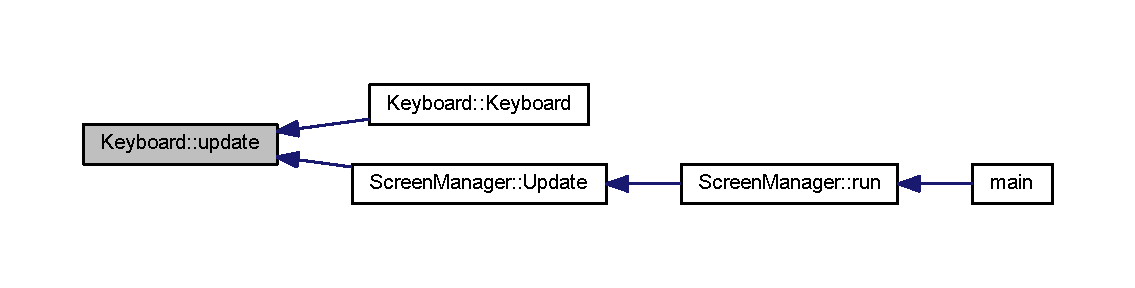
\includegraphics[width=350pt]{class_keyboard_a6410f07ddc53561a82d5328d8b330aab_icgraph}
\end{center}
\end{figure}




\subsection{Member Data Documentation}
\hypertarget{class_keyboard_a33ee9c98d3b2426fec7b69fd4f42fb9a}{\index{Keyboard@{Keyboard}!A@{A}}
\index{A@{A}!Keyboard@{Keyboard}}
\subsubsection[{A}]{\setlength{\rightskip}{0pt plus 5cm}bool Keyboard\-::\-A\hspace{0.3cm}{\ttfamily [private]}}}\label{class_keyboard_a33ee9c98d3b2426fec7b69fd4f42fb9a}
\hypertarget{class_keyboard_ae54476dd4f2f090740aa42dd230b9f24}{\index{Keyboard@{Keyboard}!Add@{Add}}
\index{Add@{Add}!Keyboard@{Keyboard}}
\subsubsection[{Add}]{\setlength{\rightskip}{0pt plus 5cm}bool Keyboard\-::\-Add\hspace{0.3cm}{\ttfamily [private]}}}\label{class_keyboard_ae54476dd4f2f090740aa42dd230b9f24}
\hypertarget{class_keyboard_a6386fea4a95993853302e9bafb520eca}{\index{Keyboard@{Keyboard}!B@{B}}
\index{B@{B}!Keyboard@{Keyboard}}
\subsubsection[{B}]{\setlength{\rightskip}{0pt plus 5cm}bool Keyboard\-::\-B\hspace{0.3cm}{\ttfamily [private]}}}\label{class_keyboard_a6386fea4a95993853302e9bafb520eca}
\hypertarget{class_keyboard_a78eb7c6bed698fe88c89ef8ce2071eab}{\index{Keyboard@{Keyboard}!Back\-Slash@{Back\-Slash}}
\index{Back\-Slash@{Back\-Slash}!Keyboard@{Keyboard}}
\subsubsection[{Back\-Slash}]{\setlength{\rightskip}{0pt plus 5cm}bool Keyboard\-::\-Back\-Slash\hspace{0.3cm}{\ttfamily [private]}}}\label{class_keyboard_a78eb7c6bed698fe88c89ef8ce2071eab}
\hypertarget{class_keyboard_adf79ea45e1815dad75cda6933a61cdc7}{\index{Keyboard@{Keyboard}!Back\-Space@{Back\-Space}}
\index{Back\-Space@{Back\-Space}!Keyboard@{Keyboard}}
\subsubsection[{Back\-Space}]{\setlength{\rightskip}{0pt plus 5cm}bool Keyboard\-::\-Back\-Space\hspace{0.3cm}{\ttfamily [private]}}}\label{class_keyboard_adf79ea45e1815dad75cda6933a61cdc7}
\hypertarget{class_keyboard_a8e9a644f450a387c8b0becfec29e0eba}{\index{Keyboard@{Keyboard}!C@{C}}
\index{C@{C}!Keyboard@{Keyboard}}
\subsubsection[{C}]{\setlength{\rightskip}{0pt plus 5cm}bool Keyboard\-::\-C\hspace{0.3cm}{\ttfamily [private]}}}\label{class_keyboard_a8e9a644f450a387c8b0becfec29e0eba}
\hypertarget{class_keyboard_a34056a5ea3c0e72446ef864a8a04cb50}{\index{Keyboard@{Keyboard}!Comma@{Comma}}
\index{Comma@{Comma}!Keyboard@{Keyboard}}
\subsubsection[{Comma}]{\setlength{\rightskip}{0pt plus 5cm}bool Keyboard\-::\-Comma\hspace{0.3cm}{\ttfamily [private]}}}\label{class_keyboard_a34056a5ea3c0e72446ef864a8a04cb50}
\hypertarget{class_keyboard_a913ff21c18119ddf7a4185c84e0e7449}{\index{Keyboard@{Keyboard}!D@{D}}
\index{D@{D}!Keyboard@{Keyboard}}
\subsubsection[{D}]{\setlength{\rightskip}{0pt plus 5cm}bool Keyboard\-::\-D\hspace{0.3cm}{\ttfamily [private]}}}\label{class_keyboard_a913ff21c18119ddf7a4185c84e0e7449}
\hypertarget{class_keyboard_a6807fa4583f3ff608a2b1d138ffdd94f}{\index{Keyboard@{Keyboard}!Dash@{Dash}}
\index{Dash@{Dash}!Keyboard@{Keyboard}}
\subsubsection[{Dash}]{\setlength{\rightskip}{0pt plus 5cm}bool Keyboard\-::\-Dash\hspace{0.3cm}{\ttfamily [private]}}}\label{class_keyboard_a6807fa4583f3ff608a2b1d138ffdd94f}
\hypertarget{class_keyboard_a12aee03fe365cff63bda09114de1f6ba}{\index{Keyboard@{Keyboard}!Delete@{Delete}}
\index{Delete@{Delete}!Keyboard@{Keyboard}}
\subsubsection[{Delete}]{\setlength{\rightskip}{0pt plus 5cm}bool Keyboard\-::\-Delete\hspace{0.3cm}{\ttfamily [private]}}}\label{class_keyboard_a12aee03fe365cff63bda09114de1f6ba}
\hypertarget{class_keyboard_ac967c214a690a18fe1868416fcba381e}{\index{Keyboard@{Keyboard}!Divide@{Divide}}
\index{Divide@{Divide}!Keyboard@{Keyboard}}
\subsubsection[{Divide}]{\setlength{\rightskip}{0pt plus 5cm}bool Keyboard\-::\-Divide\hspace{0.3cm}{\ttfamily [private]}}}\label{class_keyboard_ac967c214a690a18fe1868416fcba381e}
\hypertarget{class_keyboard_ac93e12f7dfbb6bdb55e48b4b39d13bcb}{\index{Keyboard@{Keyboard}!Down@{Down}}
\index{Down@{Down}!Keyboard@{Keyboard}}
\subsubsection[{Down}]{\setlength{\rightskip}{0pt plus 5cm}bool Keyboard\-::\-Down\hspace{0.3cm}{\ttfamily [private]}}}\label{class_keyboard_ac93e12f7dfbb6bdb55e48b4b39d13bcb}
\hypertarget{class_keyboard_a10f9fdb7927cb81bba0d054c26509a7a}{\index{Keyboard@{Keyboard}!E@{E}}
\index{E@{E}!Keyboard@{Keyboard}}
\subsubsection[{E}]{\setlength{\rightskip}{0pt plus 5cm}bool Keyboard\-::\-E\hspace{0.3cm}{\ttfamily [private]}}}\label{class_keyboard_a10f9fdb7927cb81bba0d054c26509a7a}
\hypertarget{class_keyboard_ac07897d6a729a6da93f08d8a05d51d32}{\index{Keyboard@{Keyboard}!End@{End}}
\index{End@{End}!Keyboard@{Keyboard}}
\subsubsection[{End}]{\setlength{\rightskip}{0pt plus 5cm}bool Keyboard\-::\-End\hspace{0.3cm}{\ttfamily [private]}}}\label{class_keyboard_ac07897d6a729a6da93f08d8a05d51d32}
\hypertarget{class_keyboard_a88c78877a504143da05ecc16cae24a05}{\index{Keyboard@{Keyboard}!Equal@{Equal}}
\index{Equal@{Equal}!Keyboard@{Keyboard}}
\subsubsection[{Equal}]{\setlength{\rightskip}{0pt plus 5cm}bool Keyboard\-::\-Equal\hspace{0.3cm}{\ttfamily [private]}}}\label{class_keyboard_a88c78877a504143da05ecc16cae24a05}
\hypertarget{class_keyboard_a8e951ed09368ad149881cd7b775020aa}{\index{Keyboard@{Keyboard}!Escape@{Escape}}
\index{Escape@{Escape}!Keyboard@{Keyboard}}
\subsubsection[{Escape}]{\setlength{\rightskip}{0pt plus 5cm}bool Keyboard\-::\-Escape\hspace{0.3cm}{\ttfamily [private]}}}\label{class_keyboard_a8e951ed09368ad149881cd7b775020aa}
\hypertarget{class_keyboard_af271aa6fd76947941d20934dc86a0bb2}{\index{Keyboard@{Keyboard}!F@{F}}
\index{F@{F}!Keyboard@{Keyboard}}
\subsubsection[{F}]{\setlength{\rightskip}{0pt plus 5cm}bool Keyboard\-::\-F\hspace{0.3cm}{\ttfamily [private]}}}\label{class_keyboard_af271aa6fd76947941d20934dc86a0bb2}
\hypertarget{class_keyboard_a230cedc083e5e797586368406006f715}{\index{Keyboard@{Keyboard}!F1@{F1}}
\index{F1@{F1}!Keyboard@{Keyboard}}
\subsubsection[{F1}]{\setlength{\rightskip}{0pt plus 5cm}bool Keyboard\-::\-F1\hspace{0.3cm}{\ttfamily [private]}}}\label{class_keyboard_a230cedc083e5e797586368406006f715}
\hypertarget{class_keyboard_a8841fc2609bc03c43c671943cdb7c2b3}{\index{Keyboard@{Keyboard}!F10@{F10}}
\index{F10@{F10}!Keyboard@{Keyboard}}
\subsubsection[{F10}]{\setlength{\rightskip}{0pt plus 5cm}bool Keyboard\-::\-F10\hspace{0.3cm}{\ttfamily [private]}}}\label{class_keyboard_a8841fc2609bc03c43c671943cdb7c2b3}
\hypertarget{class_keyboard_ac78bb167a053765400b29d98a99d2f0a}{\index{Keyboard@{Keyboard}!F11@{F11}}
\index{F11@{F11}!Keyboard@{Keyboard}}
\subsubsection[{F11}]{\setlength{\rightskip}{0pt plus 5cm}bool Keyboard\-::\-F11\hspace{0.3cm}{\ttfamily [private]}}}\label{class_keyboard_ac78bb167a053765400b29d98a99d2f0a}
\hypertarget{class_keyboard_a847021f30ace74ea8044195ecf4cf259}{\index{Keyboard@{Keyboard}!F12@{F12}}
\index{F12@{F12}!Keyboard@{Keyboard}}
\subsubsection[{F12}]{\setlength{\rightskip}{0pt plus 5cm}bool Keyboard\-::\-F12\hspace{0.3cm}{\ttfamily [private]}}}\label{class_keyboard_a847021f30ace74ea8044195ecf4cf259}
\hypertarget{class_keyboard_a2bd5b83f4f3dadebbb759e9770428caa}{\index{Keyboard@{Keyboard}!F13@{F13}}
\index{F13@{F13}!Keyboard@{Keyboard}}
\subsubsection[{F13}]{\setlength{\rightskip}{0pt plus 5cm}bool Keyboard\-::\-F13\hspace{0.3cm}{\ttfamily [private]}}}\label{class_keyboard_a2bd5b83f4f3dadebbb759e9770428caa}
\hypertarget{class_keyboard_ad29758ef282c8d9bf2f37aff7dd72187}{\index{Keyboard@{Keyboard}!F14@{F14}}
\index{F14@{F14}!Keyboard@{Keyboard}}
\subsubsection[{F14}]{\setlength{\rightskip}{0pt plus 5cm}bool Keyboard\-::\-F14\hspace{0.3cm}{\ttfamily [private]}}}\label{class_keyboard_ad29758ef282c8d9bf2f37aff7dd72187}
\hypertarget{class_keyboard_a46dfde14483d2a67e5da167cde929f01}{\index{Keyboard@{Keyboard}!F15@{F15}}
\index{F15@{F15}!Keyboard@{Keyboard}}
\subsubsection[{F15}]{\setlength{\rightskip}{0pt plus 5cm}bool Keyboard\-::\-F15\hspace{0.3cm}{\ttfamily [private]}}}\label{class_keyboard_a46dfde14483d2a67e5da167cde929f01}
\hypertarget{class_keyboard_a60a7dbacf30af45e575a5952a9bd3e11}{\index{Keyboard@{Keyboard}!F2@{F2}}
\index{F2@{F2}!Keyboard@{Keyboard}}
\subsubsection[{F2}]{\setlength{\rightskip}{0pt plus 5cm}bool Keyboard\-::\-F2\hspace{0.3cm}{\ttfamily [private]}}}\label{class_keyboard_a60a7dbacf30af45e575a5952a9bd3e11}
\hypertarget{class_keyboard_a4851d2aad6287c28d4be87b38715e09b}{\index{Keyboard@{Keyboard}!F3@{F3}}
\index{F3@{F3}!Keyboard@{Keyboard}}
\subsubsection[{F3}]{\setlength{\rightskip}{0pt plus 5cm}bool Keyboard\-::\-F3\hspace{0.3cm}{\ttfamily [private]}}}\label{class_keyboard_a4851d2aad6287c28d4be87b38715e09b}
\hypertarget{class_keyboard_ad567868b7540f6444aecc59a57caa0e7}{\index{Keyboard@{Keyboard}!F4@{F4}}
\index{F4@{F4}!Keyboard@{Keyboard}}
\subsubsection[{F4}]{\setlength{\rightskip}{0pt plus 5cm}bool Keyboard\-::\-F4\hspace{0.3cm}{\ttfamily [private]}}}\label{class_keyboard_ad567868b7540f6444aecc59a57caa0e7}
\hypertarget{class_keyboard_a8b6d5bd9c4d91754cea4365439c4145a}{\index{Keyboard@{Keyboard}!F5@{F5}}
\index{F5@{F5}!Keyboard@{Keyboard}}
\subsubsection[{F5}]{\setlength{\rightskip}{0pt plus 5cm}bool Keyboard\-::\-F5\hspace{0.3cm}{\ttfamily [private]}}}\label{class_keyboard_a8b6d5bd9c4d91754cea4365439c4145a}
\hypertarget{class_keyboard_a14117686ee73113ceed8b565f588eb57}{\index{Keyboard@{Keyboard}!F6@{F6}}
\index{F6@{F6}!Keyboard@{Keyboard}}
\subsubsection[{F6}]{\setlength{\rightskip}{0pt plus 5cm}bool Keyboard\-::\-F6\hspace{0.3cm}{\ttfamily [private]}}}\label{class_keyboard_a14117686ee73113ceed8b565f588eb57}
\hypertarget{class_keyboard_a27ea74cf4ee8b232d1603055c3baaf9c}{\index{Keyboard@{Keyboard}!F7@{F7}}
\index{F7@{F7}!Keyboard@{Keyboard}}
\subsubsection[{F7}]{\setlength{\rightskip}{0pt plus 5cm}bool Keyboard\-::\-F7\hspace{0.3cm}{\ttfamily [private]}}}\label{class_keyboard_a27ea74cf4ee8b232d1603055c3baaf9c}
\hypertarget{class_keyboard_a1e13ef0dff941442273b33bb27e120e5}{\index{Keyboard@{Keyboard}!F8@{F8}}
\index{F8@{F8}!Keyboard@{Keyboard}}
\subsubsection[{F8}]{\setlength{\rightskip}{0pt plus 5cm}bool Keyboard\-::\-F8\hspace{0.3cm}{\ttfamily [private]}}}\label{class_keyboard_a1e13ef0dff941442273b33bb27e120e5}
\hypertarget{class_keyboard_a6a8a5f933309045eb8b04f7fe1631f1a}{\index{Keyboard@{Keyboard}!F9@{F9}}
\index{F9@{F9}!Keyboard@{Keyboard}}
\subsubsection[{F9}]{\setlength{\rightskip}{0pt plus 5cm}bool Keyboard\-::\-F9\hspace{0.3cm}{\ttfamily [private]}}}\label{class_keyboard_a6a8a5f933309045eb8b04f7fe1631f1a}
\hypertarget{class_keyboard_a2c602997ff88ff6b54a696397e5478f9}{\index{Keyboard@{Keyboard}!G@{G}}
\index{G@{G}!Keyboard@{Keyboard}}
\subsubsection[{G}]{\setlength{\rightskip}{0pt plus 5cm}bool Keyboard\-::\-G\hspace{0.3cm}{\ttfamily [private]}}}\label{class_keyboard_a2c602997ff88ff6b54a696397e5478f9}
\hypertarget{class_keyboard_a5756caddc794320748593954cbd35a2a}{\index{Keyboard@{Keyboard}!H@{H}}
\index{H@{H}!Keyboard@{Keyboard}}
\subsubsection[{H}]{\setlength{\rightskip}{0pt plus 5cm}bool Keyboard\-::\-H\hspace{0.3cm}{\ttfamily [private]}}}\label{class_keyboard_a5756caddc794320748593954cbd35a2a}
\hypertarget{class_keyboard_a7b423efd9af41af9e712fa40bd7ac03f}{\index{Keyboard@{Keyboard}!Home@{Home}}
\index{Home@{Home}!Keyboard@{Keyboard}}
\subsubsection[{Home}]{\setlength{\rightskip}{0pt plus 5cm}bool Keyboard\-::\-Home\hspace{0.3cm}{\ttfamily [private]}}}\label{class_keyboard_a7b423efd9af41af9e712fa40bd7ac03f}
\hypertarget{class_keyboard_a59f5f1879a371a750deaef44730f6c8e}{\index{Keyboard@{Keyboard}!I@{I}}
\index{I@{I}!Keyboard@{Keyboard}}
\subsubsection[{I}]{\setlength{\rightskip}{0pt plus 5cm}bool Keyboard\-::\-I\hspace{0.3cm}{\ttfamily [private]}}}\label{class_keyboard_a59f5f1879a371a750deaef44730f6c8e}
\hypertarget{class_keyboard_adbf0d9fd5dc41eec57541d114295ca58}{\index{Keyboard@{Keyboard}!Insert@{Insert}}
\index{Insert@{Insert}!Keyboard@{Keyboard}}
\subsubsection[{Insert}]{\setlength{\rightskip}{0pt plus 5cm}bool Keyboard\-::\-Insert\hspace{0.3cm}{\ttfamily [private]}}}\label{class_keyboard_adbf0d9fd5dc41eec57541d114295ca58}
\hypertarget{class_keyboard_a79e10d1e2486a150419889ac513386b9}{\index{Keyboard@{Keyboard}!J@{J}}
\index{J@{J}!Keyboard@{Keyboard}}
\subsubsection[{J}]{\setlength{\rightskip}{0pt plus 5cm}bool Keyboard\-::\-J\hspace{0.3cm}{\ttfamily [private]}}}\label{class_keyboard_a79e10d1e2486a150419889ac513386b9}
\hypertarget{class_keyboard_a805724edf1245e28598089225bcae72e}{\index{Keyboard@{Keyboard}!K@{K}}
\index{K@{K}!Keyboard@{Keyboard}}
\subsubsection[{K}]{\setlength{\rightskip}{0pt plus 5cm}bool Keyboard\-::\-K\hspace{0.3cm}{\ttfamily [private]}}}\label{class_keyboard_a805724edf1245e28598089225bcae72e}
\hypertarget{class_keyboard_ad314cbbe55e6d9d699f9c4a3d673dc0e}{\index{Keyboard@{Keyboard}!L@{L}}
\index{L@{L}!Keyboard@{Keyboard}}
\subsubsection[{L}]{\setlength{\rightskip}{0pt plus 5cm}bool Keyboard\-::\-L\hspace{0.3cm}{\ttfamily [private]}}}\label{class_keyboard_ad314cbbe55e6d9d699f9c4a3d673dc0e}
\hypertarget{class_keyboard_a31ac170a9119716e18ceabf92679e95c}{\index{Keyboard@{Keyboard}!L\-Alt@{L\-Alt}}
\index{L\-Alt@{L\-Alt}!Keyboard@{Keyboard}}
\subsubsection[{L\-Alt}]{\setlength{\rightskip}{0pt plus 5cm}bool Keyboard\-::\-L\-Alt\hspace{0.3cm}{\ttfamily [private]}}}\label{class_keyboard_a31ac170a9119716e18ceabf92679e95c}
\hypertarget{class_keyboard_a2f9d2e47356ccdeb8cf9b6380b91c2d7}{\index{Keyboard@{Keyboard}!L\-Bracket@{L\-Bracket}}
\index{L\-Bracket@{L\-Bracket}!Keyboard@{Keyboard}}
\subsubsection[{L\-Bracket}]{\setlength{\rightskip}{0pt plus 5cm}bool Keyboard\-::\-L\-Bracket\hspace{0.3cm}{\ttfamily [private]}}}\label{class_keyboard_a2f9d2e47356ccdeb8cf9b6380b91c2d7}
\hypertarget{class_keyboard_ad17b8ff4a74d829f5eea1b87ea9fda13}{\index{Keyboard@{Keyboard}!L\-Control@{L\-Control}}
\index{L\-Control@{L\-Control}!Keyboard@{Keyboard}}
\subsubsection[{L\-Control}]{\setlength{\rightskip}{0pt plus 5cm}bool Keyboard\-::\-L\-Control\hspace{0.3cm}{\ttfamily [private]}}}\label{class_keyboard_ad17b8ff4a74d829f5eea1b87ea9fda13}
\hypertarget{class_keyboard_ac77efb57a3008e9694cc2da7b3230c77}{\index{Keyboard@{Keyboard}!Left@{Left}}
\index{Left@{Left}!Keyboard@{Keyboard}}
\subsubsection[{Left}]{\setlength{\rightskip}{0pt plus 5cm}bool Keyboard\-::\-Left\hspace{0.3cm}{\ttfamily [private]}}}\label{class_keyboard_ac77efb57a3008e9694cc2da7b3230c77}
\hypertarget{class_keyboard_a8455f8596760ac41c64d659ffa6b0c60}{\index{Keyboard@{Keyboard}!L\-Shift@{L\-Shift}}
\index{L\-Shift@{L\-Shift}!Keyboard@{Keyboard}}
\subsubsection[{L\-Shift}]{\setlength{\rightskip}{0pt plus 5cm}bool Keyboard\-::\-L\-Shift\hspace{0.3cm}{\ttfamily [private]}}}\label{class_keyboard_a8455f8596760ac41c64d659ffa6b0c60}
\hypertarget{class_keyboard_a0d39d5e2e0573e00fa0fb331baf08d39}{\index{Keyboard@{Keyboard}!L\-System@{L\-System}}
\index{L\-System@{L\-System}!Keyboard@{Keyboard}}
\subsubsection[{L\-System}]{\setlength{\rightskip}{0pt plus 5cm}bool Keyboard\-::\-L\-System\hspace{0.3cm}{\ttfamily [private]}}}\label{class_keyboard_a0d39d5e2e0573e00fa0fb331baf08d39}
\hypertarget{class_keyboard_a655e239c891a0c77273f5651f77d752b}{\index{Keyboard@{Keyboard}!M@{M}}
\index{M@{M}!Keyboard@{Keyboard}}
\subsubsection[{M}]{\setlength{\rightskip}{0pt plus 5cm}bool Keyboard\-::\-M\hspace{0.3cm}{\ttfamily [private]}}}\label{class_keyboard_a655e239c891a0c77273f5651f77d752b}
\hypertarget{class_keyboard_afaeb2278bbc8f4971d1f43cee9765900}{\index{Keyboard@{Keyboard}!Menu@{Menu}}
\index{Menu@{Menu}!Keyboard@{Keyboard}}
\subsubsection[{Menu}]{\setlength{\rightskip}{0pt plus 5cm}bool Keyboard\-::\-Menu\hspace{0.3cm}{\ttfamily [private]}}}\label{class_keyboard_afaeb2278bbc8f4971d1f43cee9765900}
\hypertarget{class_keyboard_adedf851aed90813c23d5bb1dbc81e44f}{\index{Keyboard@{Keyboard}!Multiply@{Multiply}}
\index{Multiply@{Multiply}!Keyboard@{Keyboard}}
\subsubsection[{Multiply}]{\setlength{\rightskip}{0pt plus 5cm}bool Keyboard\-::\-Multiply\hspace{0.3cm}{\ttfamily [private]}}}\label{class_keyboard_adedf851aed90813c23d5bb1dbc81e44f}
\hypertarget{class_keyboard_a9c13f7665efcec0323466f50080dd90f}{\index{Keyboard@{Keyboard}!N@{N}}
\index{N@{N}!Keyboard@{Keyboard}}
\subsubsection[{N}]{\setlength{\rightskip}{0pt plus 5cm}bool Keyboard\-::\-N\hspace{0.3cm}{\ttfamily [private]}}}\label{class_keyboard_a9c13f7665efcec0323466f50080dd90f}
\hypertarget{class_keyboard_adcaa025a0862c4ef0b915a39f095f86c}{\index{Keyboard@{Keyboard}!Num0@{Num0}}
\index{Num0@{Num0}!Keyboard@{Keyboard}}
\subsubsection[{Num0}]{\setlength{\rightskip}{0pt plus 5cm}bool Keyboard\-::\-Num0\hspace{0.3cm}{\ttfamily [private]}}}\label{class_keyboard_adcaa025a0862c4ef0b915a39f095f86c}
\hypertarget{class_keyboard_a835bf1e4085d8f539a374f38fcf44a52}{\index{Keyboard@{Keyboard}!Num1@{Num1}}
\index{Num1@{Num1}!Keyboard@{Keyboard}}
\subsubsection[{Num1}]{\setlength{\rightskip}{0pt plus 5cm}bool Keyboard\-::\-Num1\hspace{0.3cm}{\ttfamily [private]}}}\label{class_keyboard_a835bf1e4085d8f539a374f38fcf44a52}
\hypertarget{class_keyboard_af4ec2c5721ec5c013867e16d3b37dd0b}{\index{Keyboard@{Keyboard}!Num2@{Num2}}
\index{Num2@{Num2}!Keyboard@{Keyboard}}
\subsubsection[{Num2}]{\setlength{\rightskip}{0pt plus 5cm}bool Keyboard\-::\-Num2\hspace{0.3cm}{\ttfamily [private]}}}\label{class_keyboard_af4ec2c5721ec5c013867e16d3b37dd0b}
\hypertarget{class_keyboard_acd66a6febc527dd70cfec532efb4cbba}{\index{Keyboard@{Keyboard}!Num3@{Num3}}
\index{Num3@{Num3}!Keyboard@{Keyboard}}
\subsubsection[{Num3}]{\setlength{\rightskip}{0pt plus 5cm}bool Keyboard\-::\-Num3\hspace{0.3cm}{\ttfamily [private]}}}\label{class_keyboard_acd66a6febc527dd70cfec532efb4cbba}
\hypertarget{class_keyboard_a283eb8a0d196bab3d7a6cdc78152e317}{\index{Keyboard@{Keyboard}!Num4@{Num4}}
\index{Num4@{Num4}!Keyboard@{Keyboard}}
\subsubsection[{Num4}]{\setlength{\rightskip}{0pt plus 5cm}bool Keyboard\-::\-Num4\hspace{0.3cm}{\ttfamily [private]}}}\label{class_keyboard_a283eb8a0d196bab3d7a6cdc78152e317}
\hypertarget{class_keyboard_a54e89c0853c5b83cb0cb33243c161c93}{\index{Keyboard@{Keyboard}!Num5@{Num5}}
\index{Num5@{Num5}!Keyboard@{Keyboard}}
\subsubsection[{Num5}]{\setlength{\rightskip}{0pt plus 5cm}bool Keyboard\-::\-Num5\hspace{0.3cm}{\ttfamily [private]}}}\label{class_keyboard_a54e89c0853c5b83cb0cb33243c161c93}
\hypertarget{class_keyboard_aa99ba505684c08d85ab93fa340e97460}{\index{Keyboard@{Keyboard}!Num6@{Num6}}
\index{Num6@{Num6}!Keyboard@{Keyboard}}
\subsubsection[{Num6}]{\setlength{\rightskip}{0pt plus 5cm}bool Keyboard\-::\-Num6\hspace{0.3cm}{\ttfamily [private]}}}\label{class_keyboard_aa99ba505684c08d85ab93fa340e97460}
\hypertarget{class_keyboard_ab22734e5959de997b58bc1b2c8a63b1e}{\index{Keyboard@{Keyboard}!Num7@{Num7}}
\index{Num7@{Num7}!Keyboard@{Keyboard}}
\subsubsection[{Num7}]{\setlength{\rightskip}{0pt plus 5cm}bool Keyboard\-::\-Num7\hspace{0.3cm}{\ttfamily [private]}}}\label{class_keyboard_ab22734e5959de997b58bc1b2c8a63b1e}
\hypertarget{class_keyboard_a37e82bad8ef3f8a43eca409836d164bf}{\index{Keyboard@{Keyboard}!Num8@{Num8}}
\index{Num8@{Num8}!Keyboard@{Keyboard}}
\subsubsection[{Num8}]{\setlength{\rightskip}{0pt plus 5cm}bool Keyboard\-::\-Num8\hspace{0.3cm}{\ttfamily [private]}}}\label{class_keyboard_a37e82bad8ef3f8a43eca409836d164bf}
\hypertarget{class_keyboard_a946af06657d756d7a2eeebd4c7435af9}{\index{Keyboard@{Keyboard}!Num9@{Num9}}
\index{Num9@{Num9}!Keyboard@{Keyboard}}
\subsubsection[{Num9}]{\setlength{\rightskip}{0pt plus 5cm}bool Keyboard\-::\-Num9\hspace{0.3cm}{\ttfamily [private]}}}\label{class_keyboard_a946af06657d756d7a2eeebd4c7435af9}
\hypertarget{class_keyboard_abcec243a50c73730ba5e61700e2c9958}{\index{Keyboard@{Keyboard}!Numpad0@{Numpad0}}
\index{Numpad0@{Numpad0}!Keyboard@{Keyboard}}
\subsubsection[{Numpad0}]{\setlength{\rightskip}{0pt plus 5cm}bool Keyboard\-::\-Numpad0\hspace{0.3cm}{\ttfamily [private]}}}\label{class_keyboard_abcec243a50c73730ba5e61700e2c9958}
\hypertarget{class_keyboard_a7a942433aebf6d02e99dff569c2e79b2}{\index{Keyboard@{Keyboard}!Numpad1@{Numpad1}}
\index{Numpad1@{Numpad1}!Keyboard@{Keyboard}}
\subsubsection[{Numpad1}]{\setlength{\rightskip}{0pt plus 5cm}bool Keyboard\-::\-Numpad1\hspace{0.3cm}{\ttfamily [private]}}}\label{class_keyboard_a7a942433aebf6d02e99dff569c2e79b2}
\hypertarget{class_keyboard_a6d59e04f32a45b19d54d84f33fd36261}{\index{Keyboard@{Keyboard}!Numpad2@{Numpad2}}
\index{Numpad2@{Numpad2}!Keyboard@{Keyboard}}
\subsubsection[{Numpad2}]{\setlength{\rightskip}{0pt plus 5cm}bool Keyboard\-::\-Numpad2\hspace{0.3cm}{\ttfamily [private]}}}\label{class_keyboard_a6d59e04f32a45b19d54d84f33fd36261}
\hypertarget{class_keyboard_adc1b251e798213a691b706356852d437}{\index{Keyboard@{Keyboard}!Numpad3@{Numpad3}}
\index{Numpad3@{Numpad3}!Keyboard@{Keyboard}}
\subsubsection[{Numpad3}]{\setlength{\rightskip}{0pt plus 5cm}bool Keyboard\-::\-Numpad3\hspace{0.3cm}{\ttfamily [private]}}}\label{class_keyboard_adc1b251e798213a691b706356852d437}
\hypertarget{class_keyboard_a35293bca2a90c438813555c49b3d80a3}{\index{Keyboard@{Keyboard}!Numpad4@{Numpad4}}
\index{Numpad4@{Numpad4}!Keyboard@{Keyboard}}
\subsubsection[{Numpad4}]{\setlength{\rightskip}{0pt plus 5cm}bool Keyboard\-::\-Numpad4\hspace{0.3cm}{\ttfamily [private]}}}\label{class_keyboard_a35293bca2a90c438813555c49b3d80a3}
\hypertarget{class_keyboard_ac9881923cbed6c05b9b406c63a1eddb0}{\index{Keyboard@{Keyboard}!Numpad5@{Numpad5}}
\index{Numpad5@{Numpad5}!Keyboard@{Keyboard}}
\subsubsection[{Numpad5}]{\setlength{\rightskip}{0pt plus 5cm}bool Keyboard\-::\-Numpad5\hspace{0.3cm}{\ttfamily [private]}}}\label{class_keyboard_ac9881923cbed6c05b9b406c63a1eddb0}
\hypertarget{class_keyboard_ae4b1472b443fefd85324452e23c0ed29}{\index{Keyboard@{Keyboard}!Numpad6@{Numpad6}}
\index{Numpad6@{Numpad6}!Keyboard@{Keyboard}}
\subsubsection[{Numpad6}]{\setlength{\rightskip}{0pt plus 5cm}bool Keyboard\-::\-Numpad6\hspace{0.3cm}{\ttfamily [private]}}}\label{class_keyboard_ae4b1472b443fefd85324452e23c0ed29}
\hypertarget{class_keyboard_ae78f281e5bd1f8fd60539eeeee66d75d}{\index{Keyboard@{Keyboard}!Numpad7@{Numpad7}}
\index{Numpad7@{Numpad7}!Keyboard@{Keyboard}}
\subsubsection[{Numpad7}]{\setlength{\rightskip}{0pt plus 5cm}bool Keyboard\-::\-Numpad7\hspace{0.3cm}{\ttfamily [private]}}}\label{class_keyboard_ae78f281e5bd1f8fd60539eeeee66d75d}
\hypertarget{class_keyboard_a6ece43e8ea3914544e4c014f95be2f07}{\index{Keyboard@{Keyboard}!Numpad8@{Numpad8}}
\index{Numpad8@{Numpad8}!Keyboard@{Keyboard}}
\subsubsection[{Numpad8}]{\setlength{\rightskip}{0pt plus 5cm}bool Keyboard\-::\-Numpad8\hspace{0.3cm}{\ttfamily [private]}}}\label{class_keyboard_a6ece43e8ea3914544e4c014f95be2f07}
\hypertarget{class_keyboard_a5a52aa251bd832db1a472db757276e7e}{\index{Keyboard@{Keyboard}!Numpad9@{Numpad9}}
\index{Numpad9@{Numpad9}!Keyboard@{Keyboard}}
\subsubsection[{Numpad9}]{\setlength{\rightskip}{0pt plus 5cm}bool Keyboard\-::\-Numpad9\hspace{0.3cm}{\ttfamily [private]}}}\label{class_keyboard_a5a52aa251bd832db1a472db757276e7e}
\hypertarget{class_keyboard_ac2ef655c59d2d20ca9ac14b38281bd2b}{\index{Keyboard@{Keyboard}!O@{O}}
\index{O@{O}!Keyboard@{Keyboard}}
\subsubsection[{O}]{\setlength{\rightskip}{0pt plus 5cm}bool Keyboard\-::\-O\hspace{0.3cm}{\ttfamily [private]}}}\label{class_keyboard_ac2ef655c59d2d20ca9ac14b38281bd2b}
\hypertarget{class_keyboard_a0a1ccbf5bdd2ca101d91f6aeb12b0003}{\index{Keyboard@{Keyboard}!P@{P}}
\index{P@{P}!Keyboard@{Keyboard}}
\subsubsection[{P}]{\setlength{\rightskip}{0pt plus 5cm}bool Keyboard\-::\-P\hspace{0.3cm}{\ttfamily [private]}}}\label{class_keyboard_a0a1ccbf5bdd2ca101d91f6aeb12b0003}
\hypertarget{class_keyboard_a01dbe3ee9ed6e45d787ba89e7f7b8e46}{\index{Keyboard@{Keyboard}!Page\-Down@{Page\-Down}}
\index{Page\-Down@{Page\-Down}!Keyboard@{Keyboard}}
\subsubsection[{Page\-Down}]{\setlength{\rightskip}{0pt plus 5cm}bool Keyboard\-::\-Page\-Down\hspace{0.3cm}{\ttfamily [private]}}}\label{class_keyboard_a01dbe3ee9ed6e45d787ba89e7f7b8e46}
\hypertarget{class_keyboard_a7250e2957e758f84c12fe70fed725f8c}{\index{Keyboard@{Keyboard}!Page\-Up@{Page\-Up}}
\index{Page\-Up@{Page\-Up}!Keyboard@{Keyboard}}
\subsubsection[{Page\-Up}]{\setlength{\rightskip}{0pt plus 5cm}bool Keyboard\-::\-Page\-Up\hspace{0.3cm}{\ttfamily [private]}}}\label{class_keyboard_a7250e2957e758f84c12fe70fed725f8c}
\hypertarget{class_keyboard_a1b2de2903baee8b62c0dd9995b0882c1}{\index{Keyboard@{Keyboard}!Pause@{Pause}}
\index{Pause@{Pause}!Keyboard@{Keyboard}}
\subsubsection[{Pause}]{\setlength{\rightskip}{0pt plus 5cm}bool Keyboard\-::\-Pause\hspace{0.3cm}{\ttfamily [private]}}}\label{class_keyboard_a1b2de2903baee8b62c0dd9995b0882c1}
\hypertarget{class_keyboard_ab214ea962d31b8437bc0b162001574dc}{\index{Keyboard@{Keyboard}!Period@{Period}}
\index{Period@{Period}!Keyboard@{Keyboard}}
\subsubsection[{Period}]{\setlength{\rightskip}{0pt plus 5cm}bool Keyboard\-::\-Period\hspace{0.3cm}{\ttfamily [private]}}}\label{class_keyboard_ab214ea962d31b8437bc0b162001574dc}
\hypertarget{class_keyboard_a73542918c6ffdd4915925fff6aea1eb5}{\index{Keyboard@{Keyboard}!Q@{Q}}
\index{Q@{Q}!Keyboard@{Keyboard}}
\subsubsection[{Q}]{\setlength{\rightskip}{0pt plus 5cm}bool Keyboard\-::\-Q\hspace{0.3cm}{\ttfamily [private]}}}\label{class_keyboard_a73542918c6ffdd4915925fff6aea1eb5}
\hypertarget{class_keyboard_ab962f4a569eb3a171fb648c8f6df904a}{\index{Keyboard@{Keyboard}!Quote@{Quote}}
\index{Quote@{Quote}!Keyboard@{Keyboard}}
\subsubsection[{Quote}]{\setlength{\rightskip}{0pt plus 5cm}bool Keyboard\-::\-Quote\hspace{0.3cm}{\ttfamily [private]}}}\label{class_keyboard_ab962f4a569eb3a171fb648c8f6df904a}
\hypertarget{class_keyboard_a43732e3f8a2a179490d70bbca9c9cbf7}{\index{Keyboard@{Keyboard}!R@{R}}
\index{R@{R}!Keyboard@{Keyboard}}
\subsubsection[{R}]{\setlength{\rightskip}{0pt plus 5cm}bool Keyboard\-::\-R\hspace{0.3cm}{\ttfamily [private]}}}\label{class_keyboard_a43732e3f8a2a179490d70bbca9c9cbf7}
\hypertarget{class_keyboard_a7b5b72389b90761733b885ebe2feaff6}{\index{Keyboard@{Keyboard}!R\-Alt@{R\-Alt}}
\index{R\-Alt@{R\-Alt}!Keyboard@{Keyboard}}
\subsubsection[{R\-Alt}]{\setlength{\rightskip}{0pt plus 5cm}bool Keyboard\-::\-R\-Alt\hspace{0.3cm}{\ttfamily [private]}}}\label{class_keyboard_a7b5b72389b90761733b885ebe2feaff6}
\hypertarget{class_keyboard_a6924305b6bab6e1743c4f30566022e03}{\index{Keyboard@{Keyboard}!R\-Bracket@{R\-Bracket}}
\index{R\-Bracket@{R\-Bracket}!Keyboard@{Keyboard}}
\subsubsection[{R\-Bracket}]{\setlength{\rightskip}{0pt plus 5cm}bool Keyboard\-::\-R\-Bracket\hspace{0.3cm}{\ttfamily [private]}}}\label{class_keyboard_a6924305b6bab6e1743c4f30566022e03}
\hypertarget{class_keyboard_ab0b3b0b4d17a476568fe9994cf4ad92b}{\index{Keyboard@{Keyboard}!R\-Control@{R\-Control}}
\index{R\-Control@{R\-Control}!Keyboard@{Keyboard}}
\subsubsection[{R\-Control}]{\setlength{\rightskip}{0pt plus 5cm}bool Keyboard\-::\-R\-Control\hspace{0.3cm}{\ttfamily [private]}}}\label{class_keyboard_ab0b3b0b4d17a476568fe9994cf4ad92b}
\hypertarget{class_keyboard_a145aa386b22fd7c1068a336b5e7b8022}{\index{Keyboard@{Keyboard}!Return@{Return}}
\index{Return@{Return}!Keyboard@{Keyboard}}
\subsubsection[{Return}]{\setlength{\rightskip}{0pt plus 5cm}bool Keyboard\-::\-Return\hspace{0.3cm}{\ttfamily [private]}}}\label{class_keyboard_a145aa386b22fd7c1068a336b5e7b8022}
\hypertarget{class_keyboard_adf9fac46978406d8828c6699156b61d8}{\index{Keyboard@{Keyboard}!Right@{Right}}
\index{Right@{Right}!Keyboard@{Keyboard}}
\subsubsection[{Right}]{\setlength{\rightskip}{0pt plus 5cm}bool Keyboard\-::\-Right\hspace{0.3cm}{\ttfamily [private]}}}\label{class_keyboard_adf9fac46978406d8828c6699156b61d8}
\hypertarget{class_keyboard_a24b00a96a25f3bce3d1bad1e3fc2c600}{\index{Keyboard@{Keyboard}!R\-Shift@{R\-Shift}}
\index{R\-Shift@{R\-Shift}!Keyboard@{Keyboard}}
\subsubsection[{R\-Shift}]{\setlength{\rightskip}{0pt plus 5cm}bool Keyboard\-::\-R\-Shift\hspace{0.3cm}{\ttfamily [private]}}}\label{class_keyboard_a24b00a96a25f3bce3d1bad1e3fc2c600}
\hypertarget{class_keyboard_afba86b1479dfa9fb35ace002e19d6da5}{\index{Keyboard@{Keyboard}!R\-System@{R\-System}}
\index{R\-System@{R\-System}!Keyboard@{Keyboard}}
\subsubsection[{R\-System}]{\setlength{\rightskip}{0pt plus 5cm}bool Keyboard\-::\-R\-System\hspace{0.3cm}{\ttfamily [private]}}}\label{class_keyboard_afba86b1479dfa9fb35ace002e19d6da5}
\hypertarget{class_keyboard_aafafb740df9ac23e0fdbac7b85ca5902}{\index{Keyboard@{Keyboard}!S@{S}}
\index{S@{S}!Keyboard@{Keyboard}}
\subsubsection[{S}]{\setlength{\rightskip}{0pt plus 5cm}bool Keyboard\-::\-S\hspace{0.3cm}{\ttfamily [private]}}}\label{class_keyboard_aafafb740df9ac23e0fdbac7b85ca5902}
\hypertarget{class_keyboard_a630a1f3ae35be95f2a9b4da9ccec7b65}{\index{Keyboard@{Keyboard}!Semi\-Colon@{Semi\-Colon}}
\index{Semi\-Colon@{Semi\-Colon}!Keyboard@{Keyboard}}
\subsubsection[{Semi\-Colon}]{\setlength{\rightskip}{0pt plus 5cm}bool Keyboard\-::\-Semi\-Colon\hspace{0.3cm}{\ttfamily [private]}}}\label{class_keyboard_a630a1f3ae35be95f2a9b4da9ccec7b65}
\hypertarget{class_keyboard_a603303cab1a11552d040900389cfb284}{\index{Keyboard@{Keyboard}!Slash@{Slash}}
\index{Slash@{Slash}!Keyboard@{Keyboard}}
\subsubsection[{Slash}]{\setlength{\rightskip}{0pt plus 5cm}bool Keyboard\-::\-Slash\hspace{0.3cm}{\ttfamily [private]}}}\label{class_keyboard_a603303cab1a11552d040900389cfb284}
\hypertarget{class_keyboard_a26cccfd7aa8895b3ce90eef7bf78aa28}{\index{Keyboard@{Keyboard}!Space@{Space}}
\index{Space@{Space}!Keyboard@{Keyboard}}
\subsubsection[{Space}]{\setlength{\rightskip}{0pt plus 5cm}bool Keyboard\-::\-Space\hspace{0.3cm}{\ttfamily [private]}}}\label{class_keyboard_a26cccfd7aa8895b3ce90eef7bf78aa28}
\hypertarget{class_keyboard_acc099cfa6a8396bf58f59d6464a159ee}{\index{Keyboard@{Keyboard}!Subtract@{Subtract}}
\index{Subtract@{Subtract}!Keyboard@{Keyboard}}
\subsubsection[{Subtract}]{\setlength{\rightskip}{0pt plus 5cm}bool Keyboard\-::\-Subtract\hspace{0.3cm}{\ttfamily [private]}}}\label{class_keyboard_acc099cfa6a8396bf58f59d6464a159ee}
\hypertarget{class_keyboard_a82a8270c2f89be1d02deff45e5b05423}{\index{Keyboard@{Keyboard}!T@{T}}
\index{T@{T}!Keyboard@{Keyboard}}
\subsubsection[{T}]{\setlength{\rightskip}{0pt plus 5cm}bool Keyboard\-::\-T\hspace{0.3cm}{\ttfamily [private]}}}\label{class_keyboard_a82a8270c2f89be1d02deff45e5b05423}
\hypertarget{class_keyboard_a67632f0d061db111d70a6909387c61d2}{\index{Keyboard@{Keyboard}!Tab@{Tab}}
\index{Tab@{Tab}!Keyboard@{Keyboard}}
\subsubsection[{Tab}]{\setlength{\rightskip}{0pt plus 5cm}bool Keyboard\-::\-Tab\hspace{0.3cm}{\ttfamily [private]}}}\label{class_keyboard_a67632f0d061db111d70a6909387c61d2}
\hypertarget{class_keyboard_aafb679f7bd4eecbc6c7ca03e6e47e346}{\index{Keyboard@{Keyboard}!Tilde@{Tilde}}
\index{Tilde@{Tilde}!Keyboard@{Keyboard}}
\subsubsection[{Tilde}]{\setlength{\rightskip}{0pt plus 5cm}bool Keyboard\-::\-Tilde\hspace{0.3cm}{\ttfamily [private]}}}\label{class_keyboard_aafb679f7bd4eecbc6c7ca03e6e47e346}
\hypertarget{class_keyboard_a73a0cb0a587e4aea584d64486c95996b}{\index{Keyboard@{Keyboard}!U@{U}}
\index{U@{U}!Keyboard@{Keyboard}}
\subsubsection[{U}]{\setlength{\rightskip}{0pt plus 5cm}bool Keyboard\-::\-U\hspace{0.3cm}{\ttfamily [private]}}}\label{class_keyboard_a73a0cb0a587e4aea584d64486c95996b}
\hypertarget{class_keyboard_a365fe429b712c368311716ea0e6ec61a}{\index{Keyboard@{Keyboard}!Up@{Up}}
\index{Up@{Up}!Keyboard@{Keyboard}}
\subsubsection[{Up}]{\setlength{\rightskip}{0pt plus 5cm}bool Keyboard\-::\-Up\hspace{0.3cm}{\ttfamily [private]}}}\label{class_keyboard_a365fe429b712c368311716ea0e6ec61a}
\hypertarget{class_keyboard_ae41741f501d169e8671242bae37c608f}{\index{Keyboard@{Keyboard}!V@{V}}
\index{V@{V}!Keyboard@{Keyboard}}
\subsubsection[{V}]{\setlength{\rightskip}{0pt plus 5cm}bool Keyboard\-::\-V\hspace{0.3cm}{\ttfamily [private]}}}\label{class_keyboard_ae41741f501d169e8671242bae37c608f}
\hypertarget{class_keyboard_a7c1dbac444af2066b65cb5f73cfeb00e}{\index{Keyboard@{Keyboard}!W@{W}}
\index{W@{W}!Keyboard@{Keyboard}}
\subsubsection[{W}]{\setlength{\rightskip}{0pt plus 5cm}bool Keyboard\-::\-W\hspace{0.3cm}{\ttfamily [private]}}}\label{class_keyboard_a7c1dbac444af2066b65cb5f73cfeb00e}
\hypertarget{class_keyboard_afde15308c9554c8abaf8054b105b9507}{\index{Keyboard@{Keyboard}!X@{X}}
\index{X@{X}!Keyboard@{Keyboard}}
\subsubsection[{X}]{\setlength{\rightskip}{0pt plus 5cm}bool Keyboard\-::\-X\hspace{0.3cm}{\ttfamily [private]}}}\label{class_keyboard_afde15308c9554c8abaf8054b105b9507}
\hypertarget{class_keyboard_a030813b88756995bdc8b577b3674dd0a}{\index{Keyboard@{Keyboard}!Y@{Y}}
\index{Y@{Y}!Keyboard@{Keyboard}}
\subsubsection[{Y}]{\setlength{\rightskip}{0pt plus 5cm}bool Keyboard\-::\-Y\hspace{0.3cm}{\ttfamily [private]}}}\label{class_keyboard_a030813b88756995bdc8b577b3674dd0a}
\hypertarget{class_keyboard_abbae1e2f05e366553c81c136a0f3f970}{\index{Keyboard@{Keyboard}!Z@{Z}}
\index{Z@{Z}!Keyboard@{Keyboard}}
\subsubsection[{Z}]{\setlength{\rightskip}{0pt plus 5cm}bool Keyboard\-::\-Z\hspace{0.3cm}{\ttfamily [private]}}}\label{class_keyboard_abbae1e2f05e366553c81c136a0f3f970}


The documentation for this class was generated from the following files\-:\begin{DoxyCompactItemize}
\item 
D\-:/\-Users/tom/\-Documents/\-Visual Studio 2013/\-Projects/\-Revelatorframework/\-Revelator\-Framework\-\_\-\-A\-P\-I/\hyperlink{_keyboard_8hpp}{Keyboard.\-hpp}\item 
D\-:/\-Users/tom/\-Documents/\-Visual Studio 2013/\-Projects/\-Revelatorframework/\-Revelator\-Framework\-\_\-\-A\-P\-I/\hyperlink{_keyboard_8cpp}{Keyboard.\-cpp}\end{DoxyCompactItemize}

\hypertarget{class_layer}{\section{Layer Class Reference}
\label{class_layer}\index{Layer@{Layer}}
}


{\ttfamily \#include $<$Layer.\-hpp$>$}



Inheritance diagram for Layer\-:\nopagebreak
\begin{figure}[H]
\begin{center}
\leavevmode
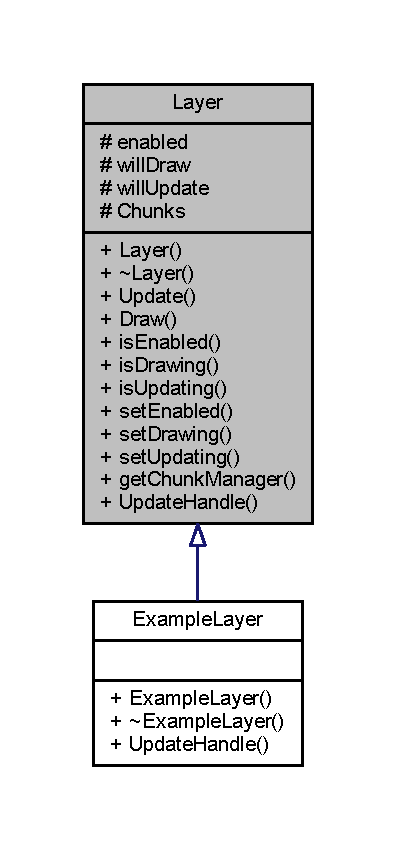
\includegraphics[width=190pt]{class_layer__inherit__graph}
\end{center}
\end{figure}


Collaboration diagram for Layer\-:\nopagebreak
\begin{figure}[H]
\begin{center}
\leavevmode
\includegraphics[height=550pt]{class_layer__coll__graph}
\end{center}
\end{figure}
\subsection*{Public Member Functions}
\begin{DoxyCompactItemize}
\item 
\hyperlink{class_layer_a8f623c7c4737dc29ecc86978d243ac6f}{Layer} ()
\item 
\hyperlink{class_layer_a1b1ba4804451dfe6cc357194e42762ae}{$\sim$\-Layer} ()
\item 
virtual void \hyperlink{class_layer_a971c3f8d301e250aded4cf0c0b9ad544}{Update} (const \hyperlink{class_update_data}{Update\-Data} \&updateobject)
\item 
virtual void \hyperlink{class_layer_a008068a5a6bd4dd274bb01bf0246cfaf}{Draw} (sf\-::\-Render\-Window \&window, sf\-::\-Vector2f offset)
\item 
bool \hyperlink{class_layer_a57c59677e3c56a7fd5e3dc985bdb9b4c}{is\-Enabled} ()
\item 
bool \hyperlink{class_layer_a46a91415e6bdc2fdb75ae0ac8498868f}{is\-Drawing} ()
\item 
bool \hyperlink{class_layer_ac2892b95b2df74446d89e4a6388f0c88}{is\-Updating} ()
\item 
void \hyperlink{class_layer_a68b9de1ac0f3eaa8274b8d0a901a825c}{set\-Enabled} (bool b)
\item 
void \hyperlink{class_layer_a0a4f62b4c031e7c2f2d5635ccd38ddd1}{set\-Drawing} (bool b)
\item 
void \hyperlink{class_layer_a0e0595efe93dbd63b05339f35399d1ad}{set\-Updating} (bool b)
\item 
\hyperlink{class_chunk_manager}{Chunk\-Manager} $\ast$ \hyperlink{class_layer_afbfd549c4d1da2e4a2d78a33586c95e1}{get\-Chunk\-Manager} ()
\item 
virtual void \hyperlink{class_layer_a1e7a6db5ee252c8ea9c44a21aaf2b0c9}{Update\-Handle} (const \hyperlink{class_update_data}{Update\-Data} \&updateobject)=0
\end{DoxyCompactItemize}
\subsection*{Protected Attributes}
\begin{DoxyCompactItemize}
\item 
bool \hyperlink{class_layer_af9f9c9a8c4a053bd829a06273df297bd}{enabled}
\item 
bool \hyperlink{class_layer_a64902a81921ba2fc792d044392b14ecc}{will\-Draw}
\item 
bool \hyperlink{class_layer_a8c3badeb437135a265c931f4ee728a48}{will\-Update}
\item 
\hyperlink{class_chunk_manager}{Chunk\-Manager} $\ast$ \hyperlink{class_layer_ab5408f6d27ad51d73df507296f16c811}{Chunks}
\end{DoxyCompactItemize}


\subsection{Constructor \& Destructor Documentation}
\hypertarget{class_layer_a8f623c7c4737dc29ecc86978d243ac6f}{\index{Layer@{Layer}!Layer@{Layer}}
\index{Layer@{Layer}!Layer@{Layer}}
\subsubsection[{Layer}]{\setlength{\rightskip}{0pt plus 5cm}Layer\-::\-Layer (
\begin{DoxyParamCaption}
{}
\end{DoxyParamCaption}
)}}\label{class_layer_a8f623c7c4737dc29ecc86978d243ac6f}
\hypertarget{class_layer_a1b1ba4804451dfe6cc357194e42762ae}{\index{Layer@{Layer}!$\sim$\-Layer@{$\sim$\-Layer}}
\index{$\sim$\-Layer@{$\sim$\-Layer}!Layer@{Layer}}
\subsubsection[{$\sim$\-Layer}]{\setlength{\rightskip}{0pt plus 5cm}Layer\-::$\sim$\-Layer (
\begin{DoxyParamCaption}
{}
\end{DoxyParamCaption}
)}}\label{class_layer_a1b1ba4804451dfe6cc357194e42762ae}


\subsection{Member Function Documentation}
\hypertarget{class_layer_a008068a5a6bd4dd274bb01bf0246cfaf}{\index{Layer@{Layer}!Draw@{Draw}}
\index{Draw@{Draw}!Layer@{Layer}}
\subsubsection[{Draw}]{\setlength{\rightskip}{0pt plus 5cm}void Layer\-::\-Draw (
\begin{DoxyParamCaption}
\item[{sf\-::\-Render\-Window \&}]{window, }
\item[{sf\-::\-Vector2f}]{offset}
\end{DoxyParamCaption}
)\hspace{0.3cm}{\ttfamily [virtual]}}}\label{class_layer_a008068a5a6bd4dd274bb01bf0246cfaf}


Here is the call graph for this function\-:\nopagebreak
\begin{figure}[H]
\begin{center}
\leavevmode
\includegraphics[width=350pt]{class_layer_a008068a5a6bd4dd274bb01bf0246cfaf_cgraph}
\end{center}
\end{figure}


\hypertarget{class_layer_afbfd549c4d1da2e4a2d78a33586c95e1}{\index{Layer@{Layer}!get\-Chunk\-Manager@{get\-Chunk\-Manager}}
\index{get\-Chunk\-Manager@{get\-Chunk\-Manager}!Layer@{Layer}}
\subsubsection[{get\-Chunk\-Manager}]{\setlength{\rightskip}{0pt plus 5cm}{\bf Chunk\-Manager}$\ast$ Layer\-::get\-Chunk\-Manager (
\begin{DoxyParamCaption}
{}
\end{DoxyParamCaption}
)\hspace{0.3cm}{\ttfamily [inline]}}}\label{class_layer_afbfd549c4d1da2e4a2d78a33586c95e1}


Here is the caller graph for this function\-:\nopagebreak
\begin{figure}[H]
\begin{center}
\leavevmode
\includegraphics[width=350pt]{class_layer_afbfd549c4d1da2e4a2d78a33586c95e1_icgraph}
\end{center}
\end{figure}


\hypertarget{class_layer_a46a91415e6bdc2fdb75ae0ac8498868f}{\index{Layer@{Layer}!is\-Drawing@{is\-Drawing}}
\index{is\-Drawing@{is\-Drawing}!Layer@{Layer}}
\subsubsection[{is\-Drawing}]{\setlength{\rightskip}{0pt plus 5cm}bool Layer\-::is\-Drawing (
\begin{DoxyParamCaption}
{}
\end{DoxyParamCaption}
)\hspace{0.3cm}{\ttfamily [inline]}}}\label{class_layer_a46a91415e6bdc2fdb75ae0ac8498868f}
\hypertarget{class_layer_a57c59677e3c56a7fd5e3dc985bdb9b4c}{\index{Layer@{Layer}!is\-Enabled@{is\-Enabled}}
\index{is\-Enabled@{is\-Enabled}!Layer@{Layer}}
\subsubsection[{is\-Enabled}]{\setlength{\rightskip}{0pt plus 5cm}bool Layer\-::is\-Enabled (
\begin{DoxyParamCaption}
{}
\end{DoxyParamCaption}
)\hspace{0.3cm}{\ttfamily [inline]}}}\label{class_layer_a57c59677e3c56a7fd5e3dc985bdb9b4c}
\hypertarget{class_layer_ac2892b95b2df74446d89e4a6388f0c88}{\index{Layer@{Layer}!is\-Updating@{is\-Updating}}
\index{is\-Updating@{is\-Updating}!Layer@{Layer}}
\subsubsection[{is\-Updating}]{\setlength{\rightskip}{0pt plus 5cm}bool Layer\-::is\-Updating (
\begin{DoxyParamCaption}
{}
\end{DoxyParamCaption}
)\hspace{0.3cm}{\ttfamily [inline]}}}\label{class_layer_ac2892b95b2df74446d89e4a6388f0c88}
\hypertarget{class_layer_a0a4f62b4c031e7c2f2d5635ccd38ddd1}{\index{Layer@{Layer}!set\-Drawing@{set\-Drawing}}
\index{set\-Drawing@{set\-Drawing}!Layer@{Layer}}
\subsubsection[{set\-Drawing}]{\setlength{\rightskip}{0pt plus 5cm}void Layer\-::set\-Drawing (
\begin{DoxyParamCaption}
\item[{bool}]{b}
\end{DoxyParamCaption}
)\hspace{0.3cm}{\ttfamily [inline]}}}\label{class_layer_a0a4f62b4c031e7c2f2d5635ccd38ddd1}


Here is the caller graph for this function\-:\nopagebreak
\begin{figure}[H]
\begin{center}
\leavevmode
\includegraphics[width=350pt]{class_layer_a0a4f62b4c031e7c2f2d5635ccd38ddd1_icgraph}
\end{center}
\end{figure}


\hypertarget{class_layer_a68b9de1ac0f3eaa8274b8d0a901a825c}{\index{Layer@{Layer}!set\-Enabled@{set\-Enabled}}
\index{set\-Enabled@{set\-Enabled}!Layer@{Layer}}
\subsubsection[{set\-Enabled}]{\setlength{\rightskip}{0pt plus 5cm}void Layer\-::set\-Enabled (
\begin{DoxyParamCaption}
\item[{bool}]{b}
\end{DoxyParamCaption}
)\hspace{0.3cm}{\ttfamily [inline]}}}\label{class_layer_a68b9de1ac0f3eaa8274b8d0a901a825c}


Here is the caller graph for this function\-:\nopagebreak
\begin{figure}[H]
\begin{center}
\leavevmode
\includegraphics[width=350pt]{class_layer_a68b9de1ac0f3eaa8274b8d0a901a825c_icgraph}
\end{center}
\end{figure}


\hypertarget{class_layer_a0e0595efe93dbd63b05339f35399d1ad}{\index{Layer@{Layer}!set\-Updating@{set\-Updating}}
\index{set\-Updating@{set\-Updating}!Layer@{Layer}}
\subsubsection[{set\-Updating}]{\setlength{\rightskip}{0pt plus 5cm}void Layer\-::set\-Updating (
\begin{DoxyParamCaption}
\item[{bool}]{b}
\end{DoxyParamCaption}
)\hspace{0.3cm}{\ttfamily [inline]}}}\label{class_layer_a0e0595efe93dbd63b05339f35399d1ad}


Here is the caller graph for this function\-:\nopagebreak
\begin{figure}[H]
\begin{center}
\leavevmode
\includegraphics[width=350pt]{class_layer_a0e0595efe93dbd63b05339f35399d1ad_icgraph}
\end{center}
\end{figure}


\hypertarget{class_layer_a971c3f8d301e250aded4cf0c0b9ad544}{\index{Layer@{Layer}!Update@{Update}}
\index{Update@{Update}!Layer@{Layer}}
\subsubsection[{Update}]{\setlength{\rightskip}{0pt plus 5cm}void Layer\-::\-Update (
\begin{DoxyParamCaption}
\item[{const {\bf Update\-Data} \&}]{updateobject}
\end{DoxyParamCaption}
)\hspace{0.3cm}{\ttfamily [virtual]}}}\label{class_layer_a971c3f8d301e250aded4cf0c0b9ad544}


Here is the call graph for this function\-:\nopagebreak
\begin{figure}[H]
\begin{center}
\leavevmode
\includegraphics[width=350pt]{class_layer_a971c3f8d301e250aded4cf0c0b9ad544_cgraph}
\end{center}
\end{figure}


\hypertarget{class_layer_a1e7a6db5ee252c8ea9c44a21aaf2b0c9}{\index{Layer@{Layer}!Update\-Handle@{Update\-Handle}}
\index{Update\-Handle@{Update\-Handle}!Layer@{Layer}}
\subsubsection[{Update\-Handle}]{\setlength{\rightskip}{0pt plus 5cm}virtual void Layer\-::\-Update\-Handle (
\begin{DoxyParamCaption}
\item[{const {\bf Update\-Data} \&}]{updateobject}
\end{DoxyParamCaption}
)\hspace{0.3cm}{\ttfamily [pure virtual]}}}\label{class_layer_a1e7a6db5ee252c8ea9c44a21aaf2b0c9}


Implemented in \hyperlink{class_example_layer_a97b36d082a4b5dd7e145773fca666490}{Example\-Layer}.



\subsection{Member Data Documentation}
\hypertarget{class_layer_ab5408f6d27ad51d73df507296f16c811}{\index{Layer@{Layer}!Chunks@{Chunks}}
\index{Chunks@{Chunks}!Layer@{Layer}}
\subsubsection[{Chunks}]{\setlength{\rightskip}{0pt plus 5cm}{\bf Chunk\-Manager}$\ast$ Layer\-::\-Chunks\hspace{0.3cm}{\ttfamily [protected]}}}\label{class_layer_ab5408f6d27ad51d73df507296f16c811}
\hypertarget{class_layer_af9f9c9a8c4a053bd829a06273df297bd}{\index{Layer@{Layer}!enabled@{enabled}}
\index{enabled@{enabled}!Layer@{Layer}}
\subsubsection[{enabled}]{\setlength{\rightskip}{0pt plus 5cm}bool Layer\-::enabled\hspace{0.3cm}{\ttfamily [protected]}}}\label{class_layer_af9f9c9a8c4a053bd829a06273df297bd}
\hypertarget{class_layer_a64902a81921ba2fc792d044392b14ecc}{\index{Layer@{Layer}!will\-Draw@{will\-Draw}}
\index{will\-Draw@{will\-Draw}!Layer@{Layer}}
\subsubsection[{will\-Draw}]{\setlength{\rightskip}{0pt plus 5cm}bool Layer\-::will\-Draw\hspace{0.3cm}{\ttfamily [protected]}}}\label{class_layer_a64902a81921ba2fc792d044392b14ecc}
\hypertarget{class_layer_a8c3badeb437135a265c931f4ee728a48}{\index{Layer@{Layer}!will\-Update@{will\-Update}}
\index{will\-Update@{will\-Update}!Layer@{Layer}}
\subsubsection[{will\-Update}]{\setlength{\rightskip}{0pt plus 5cm}bool Layer\-::will\-Update\hspace{0.3cm}{\ttfamily [protected]}}}\label{class_layer_a8c3badeb437135a265c931f4ee728a48}


The documentation for this class was generated from the following files\-:\begin{DoxyCompactItemize}
\item 
D\-:/\-Users/tom/\-Documents/\-Visual Studio 2013/\-Projects/\-Revelatorframework/\-Revelator\-Framework\-\_\-\-A\-P\-I/\hyperlink{_layer_8hpp}{Layer.\-hpp}\item 
D\-:/\-Users/tom/\-Documents/\-Visual Studio 2013/\-Projects/\-Revelatorframework/\-Revelator\-Framework\-\_\-\-A\-P\-I/\hyperlink{_layer_8cpp}{Layer.\-cpp}\end{DoxyCompactItemize}

\hypertarget{class_layer_producer}{\section{Layer\-Producer Class Reference}
\label{class_layer_producer}\index{Layer\-Producer@{Layer\-Producer}}
}


{\ttfamily \#include $<$Layer\-Producer.\-hpp$>$}



Inheritance diagram for Layer\-Producer\-:\nopagebreak
\begin{figure}[H]
\begin{center}
\leavevmode
\includegraphics[width=219pt]{class_layer_producer__inherit__graph}
\end{center}
\end{figure}


Collaboration diagram for Layer\-Producer\-:\nopagebreak
\begin{figure}[H]
\begin{center}
\leavevmode
\includegraphics[width=181pt]{class_layer_producer__coll__graph}
\end{center}
\end{figure}
\subsection*{Public Member Functions}
\begin{DoxyCompactItemize}
\item 
\hyperlink{class_layer_producer_a0301ebdf75429cfd1815ded361ff655f}{Layer\-Producer} ()
\item 
\hyperlink{class_layer_producer_a7b3ed114fd9cae6ee77ccead38066d3b}{$\sim$\-Layer\-Producer} ()
\item 
virtual \hyperlink{class_layer}{Layer} $\ast$ \hyperlink{class_layer_producer_a80eaa2d71da1e4b9150a14c92516d3e2}{Produce} ()=0
\item 
virtual \hyperlink{class_layer}{Layer} $\ast$ \hyperlink{class_layer_producer_a20ffa919098cda78577d64bffccc3680}{Produce} (\hyperlink{class_producer_package}{Producer\-Package} Package)=0
\item 
virtual \hyperlink{class_layer}{Layer} $\ast$ \hyperlink{class_layer_producer_a39650cad3ffe7017b51637072937e65a}{Produce} (\hyperlink{class_producer_package}{Producer\-Package} $\ast$Package)=0
\end{DoxyCompactItemize}


\subsection{Constructor \& Destructor Documentation}
\hypertarget{class_layer_producer_a0301ebdf75429cfd1815ded361ff655f}{\index{Layer\-Producer@{Layer\-Producer}!Layer\-Producer@{Layer\-Producer}}
\index{Layer\-Producer@{Layer\-Producer}!LayerProducer@{Layer\-Producer}}
\subsubsection[{Layer\-Producer}]{\setlength{\rightskip}{0pt plus 5cm}Layer\-Producer\-::\-Layer\-Producer (
\begin{DoxyParamCaption}
{}
\end{DoxyParamCaption}
)}}\label{class_layer_producer_a0301ebdf75429cfd1815ded361ff655f}
\hypertarget{class_layer_producer_a7b3ed114fd9cae6ee77ccead38066d3b}{\index{Layer\-Producer@{Layer\-Producer}!$\sim$\-Layer\-Producer@{$\sim$\-Layer\-Producer}}
\index{$\sim$\-Layer\-Producer@{$\sim$\-Layer\-Producer}!LayerProducer@{Layer\-Producer}}
\subsubsection[{$\sim$\-Layer\-Producer}]{\setlength{\rightskip}{0pt plus 5cm}Layer\-Producer\-::$\sim$\-Layer\-Producer (
\begin{DoxyParamCaption}
{}
\end{DoxyParamCaption}
)}}\label{class_layer_producer_a7b3ed114fd9cae6ee77ccead38066d3b}


\subsection{Member Function Documentation}
\hypertarget{class_layer_producer_a80eaa2d71da1e4b9150a14c92516d3e2}{\index{Layer\-Producer@{Layer\-Producer}!Produce@{Produce}}
\index{Produce@{Produce}!LayerProducer@{Layer\-Producer}}
\subsubsection[{Produce}]{\setlength{\rightskip}{0pt plus 5cm}virtual {\bf Layer}$\ast$ Layer\-Producer\-::\-Produce (
\begin{DoxyParamCaption}
{}
\end{DoxyParamCaption}
)\hspace{0.3cm}{\ttfamily [pure virtual]}}}\label{class_layer_producer_a80eaa2d71da1e4b9150a14c92516d3e2}


Implemented in \hyperlink{class_example_layer_producer_add9cb70333ae10c7a1c58d7e4d8f64fc}{Example\-Layer\-Producer}.

\hypertarget{class_layer_producer_a20ffa919098cda78577d64bffccc3680}{\index{Layer\-Producer@{Layer\-Producer}!Produce@{Produce}}
\index{Produce@{Produce}!LayerProducer@{Layer\-Producer}}
\subsubsection[{Produce}]{\setlength{\rightskip}{0pt plus 5cm}virtual {\bf Layer}$\ast$ Layer\-Producer\-::\-Produce (
\begin{DoxyParamCaption}
\item[{{\bf Producer\-Package}}]{Package}
\end{DoxyParamCaption}
)\hspace{0.3cm}{\ttfamily [pure virtual]}}}\label{class_layer_producer_a20ffa919098cda78577d64bffccc3680}


Implemented in \hyperlink{class_example_layer_producer_adb3d15b45aeaaebcf381c33972858811}{Example\-Layer\-Producer}.

\hypertarget{class_layer_producer_a39650cad3ffe7017b51637072937e65a}{\index{Layer\-Producer@{Layer\-Producer}!Produce@{Produce}}
\index{Produce@{Produce}!LayerProducer@{Layer\-Producer}}
\subsubsection[{Produce}]{\setlength{\rightskip}{0pt plus 5cm}virtual {\bf Layer}$\ast$ Layer\-Producer\-::\-Produce (
\begin{DoxyParamCaption}
\item[{{\bf Producer\-Package} $\ast$}]{Package}
\end{DoxyParamCaption}
)\hspace{0.3cm}{\ttfamily [pure virtual]}}}\label{class_layer_producer_a39650cad3ffe7017b51637072937e65a}


Implemented in \hyperlink{class_example_layer_producer_a580af18f887042b6ef9170f92ee14b8e}{Example\-Layer\-Producer}.



The documentation for this class was generated from the following files\-:\begin{DoxyCompactItemize}
\item 
D\-:/\-Users/tom/\-Documents/\-Visual Studio 2013/\-Projects/\-Revelatorframework/\-Revelator\-Framework\-\_\-\-A\-P\-I/\hyperlink{_layer_producer_8hpp}{Layer\-Producer.\-hpp}\item 
D\-:/\-Users/tom/\-Documents/\-Visual Studio 2013/\-Projects/\-Revelatorframework/\-Revelator\-Framework\-\_\-\-A\-P\-I/\hyperlink{_layer_producer_8cpp}{Layer\-Producer.\-cpp}\end{DoxyCompactItemize}

\hypertarget{class_mouse}{\section{Mouse Class Reference}
\label{class_mouse}\index{Mouse@{Mouse}}
}


{\ttfamily \#include $<$Mouse.\-hpp$>$}



Collaboration diagram for Mouse\-:\nopagebreak
\begin{figure}[H]
\begin{center}
\leavevmode
\includegraphics[width=190pt]{class_mouse__coll__graph}
\end{center}
\end{figure}
\subsection*{Public Member Functions}
\begin{DoxyCompactItemize}
\item 
\hyperlink{class_mouse_afdf7d8abef29c10be77ead773f964f4f}{$\sim$\-Mouse} ()
\item 
\hyperlink{class_mouse_a6c87ac5e0784ef185d003486c0cd97a7}{Mouse} (const \hyperlink{class_mouse}{Mouse} \&mouse)=delete
\item 
\hyperlink{class_mouse}{Mouse} \& \hyperlink{class_mouse_a0ba383d1a0ed97fcc7133baeb13dffb9}{operator=} (const \hyperlink{class_mouse}{Mouse} \&mouse)=delete
\item 
bool \hyperlink{class_mouse_aba7bc3e6f4ea41b41d983300cafe94e3}{get\-Left} ()
\item 
bool \hyperlink{class_mouse_a57a56ce6e0c3dee5399dd8bd317f0300}{get\-Right} ()
\item 
bool \hyperlink{class_mouse_a971194f66c07663aa9d9a1f3256a459e}{get\-Middle} ()
\item 
bool \hyperlink{class_mouse_a34e7edee2f57d2b4284e12946b945392}{get\-X\-Button1} ()
\item 
bool \hyperlink{class_mouse_a4f61c34b9a79970983c2151698481b35}{get\-X\-Button2} ()
\item 
sf\-::\-Vector2f \hyperlink{class_mouse_a96a1dc1c7d7edf64110f8bc4795966e2}{get\-Mouse\-Position} ()
\item 
void \hyperlink{class_mouse_add9756fabb1ae55d56e10b930e5592b6}{Update} ()
\end{DoxyCompactItemize}
\subsection*{Static Public Member Functions}
\begin{DoxyCompactItemize}
\item 
static \hyperlink{class_mouse}{Mouse} \& \hyperlink{class_mouse_a96ed80e3232b68b34368c8f1f79f5cff}{get\-Instance} ()
\end{DoxyCompactItemize}
\subsection*{Private Member Functions}
\begin{DoxyCompactItemize}
\item 
\hyperlink{class_mouse_a99024d3700d649ae19c1537b42a3e86d}{Mouse} ()
\end{DoxyCompactItemize}
\subsection*{Private Attributes}
\begin{DoxyCompactItemize}
\item 
bool \hyperlink{class_mouse_ace644d872e798ce789726ec958236428}{Mouse\-Left}
\item 
bool \hyperlink{class_mouse_a0d7dd53605221594b161f9d8e61aa345}{Mouse\-Right}
\item 
bool \hyperlink{class_mouse_a4cbf96ff26822cc0eb8ea3f73a9edc9a}{Mouse\-Middle}
\item 
bool \hyperlink{class_mouse_af909f12e58b2b80528c5ca05d0452bda}{Mouse\-X\-Button1}
\item 
bool \hyperlink{class_mouse_ade6dd013286bf4829948f8a69d9b7f8a}{Mouse\-X\-Button2}
\item 
sf\-::\-Vector2f \hyperlink{class_mouse_ae83f237e6ca4e0f366eb6f1a03964886}{Mouse\-Position}
\end{DoxyCompactItemize}


\subsection{Constructor \& Destructor Documentation}
\hypertarget{class_mouse_afdf7d8abef29c10be77ead773f964f4f}{\index{Mouse@{Mouse}!$\sim$\-Mouse@{$\sim$\-Mouse}}
\index{$\sim$\-Mouse@{$\sim$\-Mouse}!Mouse@{Mouse}}
\subsubsection[{$\sim$\-Mouse}]{\setlength{\rightskip}{0pt plus 5cm}Mouse\-::$\sim$\-Mouse (
\begin{DoxyParamCaption}
{}
\end{DoxyParamCaption}
)}}\label{class_mouse_afdf7d8abef29c10be77ead773f964f4f}
\hypertarget{class_mouse_a6c87ac5e0784ef185d003486c0cd97a7}{\index{Mouse@{Mouse}!Mouse@{Mouse}}
\index{Mouse@{Mouse}!Mouse@{Mouse}}
\subsubsection[{Mouse}]{\setlength{\rightskip}{0pt plus 5cm}Mouse\-::\-Mouse (
\begin{DoxyParamCaption}
\item[{const {\bf Mouse} \&}]{mouse}
\end{DoxyParamCaption}
)\hspace{0.3cm}{\ttfamily [delete]}}}\label{class_mouse_a6c87ac5e0784ef185d003486c0cd97a7}
\hypertarget{class_mouse_a99024d3700d649ae19c1537b42a3e86d}{\index{Mouse@{Mouse}!Mouse@{Mouse}}
\index{Mouse@{Mouse}!Mouse@{Mouse}}
\subsubsection[{Mouse}]{\setlength{\rightskip}{0pt plus 5cm}Mouse\-::\-Mouse (
\begin{DoxyParamCaption}
{}
\end{DoxyParamCaption}
)\hspace{0.3cm}{\ttfamily [private]}}}\label{class_mouse_a99024d3700d649ae19c1537b42a3e86d}


Here is the call graph for this function\-:\nopagebreak
\begin{figure}[H]
\begin{center}
\leavevmode
\includegraphics[width=280pt]{class_mouse_a99024d3700d649ae19c1537b42a3e86d_cgraph}
\end{center}
\end{figure}




\subsection{Member Function Documentation}
\hypertarget{class_mouse_a96ed80e3232b68b34368c8f1f79f5cff}{\index{Mouse@{Mouse}!get\-Instance@{get\-Instance}}
\index{get\-Instance@{get\-Instance}!Mouse@{Mouse}}
\subsubsection[{get\-Instance}]{\setlength{\rightskip}{0pt plus 5cm}{\bf Mouse} \& Mouse\-::get\-Instance (
\begin{DoxyParamCaption}
{}
\end{DoxyParamCaption}
)\hspace{0.3cm}{\ttfamily [static]}}}\label{class_mouse_a96ed80e3232b68b34368c8f1f79f5cff}


Here is the caller graph for this function\-:\nopagebreak
\begin{figure}[H]
\begin{center}
\leavevmode
\includegraphics[width=350pt]{class_mouse_a96ed80e3232b68b34368c8f1f79f5cff_icgraph}
\end{center}
\end{figure}


\hypertarget{class_mouse_aba7bc3e6f4ea41b41d983300cafe94e3}{\index{Mouse@{Mouse}!get\-Left@{get\-Left}}
\index{get\-Left@{get\-Left}!Mouse@{Mouse}}
\subsubsection[{get\-Left}]{\setlength{\rightskip}{0pt plus 5cm}bool Mouse\-::get\-Left (
\begin{DoxyParamCaption}
{}
\end{DoxyParamCaption}
)\hspace{0.3cm}{\ttfamily [inline]}}}\label{class_mouse_aba7bc3e6f4ea41b41d983300cafe94e3}
\hypertarget{class_mouse_a971194f66c07663aa9d9a1f3256a459e}{\index{Mouse@{Mouse}!get\-Middle@{get\-Middle}}
\index{get\-Middle@{get\-Middle}!Mouse@{Mouse}}
\subsubsection[{get\-Middle}]{\setlength{\rightskip}{0pt plus 5cm}bool Mouse\-::get\-Middle (
\begin{DoxyParamCaption}
{}
\end{DoxyParamCaption}
)\hspace{0.3cm}{\ttfamily [inline]}}}\label{class_mouse_a971194f66c07663aa9d9a1f3256a459e}
\hypertarget{class_mouse_a96a1dc1c7d7edf64110f8bc4795966e2}{\index{Mouse@{Mouse}!get\-Mouse\-Position@{get\-Mouse\-Position}}
\index{get\-Mouse\-Position@{get\-Mouse\-Position}!Mouse@{Mouse}}
\subsubsection[{get\-Mouse\-Position}]{\setlength{\rightskip}{0pt plus 5cm}sf\-::\-Vector2f Mouse\-::get\-Mouse\-Position (
\begin{DoxyParamCaption}
{}
\end{DoxyParamCaption}
)\hspace{0.3cm}{\ttfamily [inline]}}}\label{class_mouse_a96a1dc1c7d7edf64110f8bc4795966e2}
\hypertarget{class_mouse_a57a56ce6e0c3dee5399dd8bd317f0300}{\index{Mouse@{Mouse}!get\-Right@{get\-Right}}
\index{get\-Right@{get\-Right}!Mouse@{Mouse}}
\subsubsection[{get\-Right}]{\setlength{\rightskip}{0pt plus 5cm}bool Mouse\-::get\-Right (
\begin{DoxyParamCaption}
{}
\end{DoxyParamCaption}
)\hspace{0.3cm}{\ttfamily [inline]}}}\label{class_mouse_a57a56ce6e0c3dee5399dd8bd317f0300}
\hypertarget{class_mouse_a34e7edee2f57d2b4284e12946b945392}{\index{Mouse@{Mouse}!get\-X\-Button1@{get\-X\-Button1}}
\index{get\-X\-Button1@{get\-X\-Button1}!Mouse@{Mouse}}
\subsubsection[{get\-X\-Button1}]{\setlength{\rightskip}{0pt plus 5cm}bool Mouse\-::get\-X\-Button1 (
\begin{DoxyParamCaption}
{}
\end{DoxyParamCaption}
)\hspace{0.3cm}{\ttfamily [inline]}}}\label{class_mouse_a34e7edee2f57d2b4284e12946b945392}
\hypertarget{class_mouse_a4f61c34b9a79970983c2151698481b35}{\index{Mouse@{Mouse}!get\-X\-Button2@{get\-X\-Button2}}
\index{get\-X\-Button2@{get\-X\-Button2}!Mouse@{Mouse}}
\subsubsection[{get\-X\-Button2}]{\setlength{\rightskip}{0pt plus 5cm}bool Mouse\-::get\-X\-Button2 (
\begin{DoxyParamCaption}
{}
\end{DoxyParamCaption}
)\hspace{0.3cm}{\ttfamily [inline]}}}\label{class_mouse_a4f61c34b9a79970983c2151698481b35}
\hypertarget{class_mouse_a0ba383d1a0ed97fcc7133baeb13dffb9}{\index{Mouse@{Mouse}!operator=@{operator=}}
\index{operator=@{operator=}!Mouse@{Mouse}}
\subsubsection[{operator=}]{\setlength{\rightskip}{0pt plus 5cm}{\bf Mouse}\& Mouse\-::operator= (
\begin{DoxyParamCaption}
\item[{const {\bf Mouse} \&}]{mouse}
\end{DoxyParamCaption}
)\hspace{0.3cm}{\ttfamily [delete]}}}\label{class_mouse_a0ba383d1a0ed97fcc7133baeb13dffb9}
\hypertarget{class_mouse_add9756fabb1ae55d56e10b930e5592b6}{\index{Mouse@{Mouse}!Update@{Update}}
\index{Update@{Update}!Mouse@{Mouse}}
\subsubsection[{Update}]{\setlength{\rightskip}{0pt plus 5cm}void Mouse\-::\-Update (
\begin{DoxyParamCaption}
{}
\end{DoxyParamCaption}
)}}\label{class_mouse_add9756fabb1ae55d56e10b930e5592b6}


Here is the caller graph for this function\-:\nopagebreak
\begin{figure}[H]
\begin{center}
\leavevmode
\includegraphics[width=350pt]{class_mouse_add9756fabb1ae55d56e10b930e5592b6_icgraph}
\end{center}
\end{figure}




\subsection{Member Data Documentation}
\hypertarget{class_mouse_ace644d872e798ce789726ec958236428}{\index{Mouse@{Mouse}!Mouse\-Left@{Mouse\-Left}}
\index{Mouse\-Left@{Mouse\-Left}!Mouse@{Mouse}}
\subsubsection[{Mouse\-Left}]{\setlength{\rightskip}{0pt plus 5cm}bool Mouse\-::\-Mouse\-Left\hspace{0.3cm}{\ttfamily [private]}}}\label{class_mouse_ace644d872e798ce789726ec958236428}
\hypertarget{class_mouse_a4cbf96ff26822cc0eb8ea3f73a9edc9a}{\index{Mouse@{Mouse}!Mouse\-Middle@{Mouse\-Middle}}
\index{Mouse\-Middle@{Mouse\-Middle}!Mouse@{Mouse}}
\subsubsection[{Mouse\-Middle}]{\setlength{\rightskip}{0pt plus 5cm}bool Mouse\-::\-Mouse\-Middle\hspace{0.3cm}{\ttfamily [private]}}}\label{class_mouse_a4cbf96ff26822cc0eb8ea3f73a9edc9a}
\hypertarget{class_mouse_ae83f237e6ca4e0f366eb6f1a03964886}{\index{Mouse@{Mouse}!Mouse\-Position@{Mouse\-Position}}
\index{Mouse\-Position@{Mouse\-Position}!Mouse@{Mouse}}
\subsubsection[{Mouse\-Position}]{\setlength{\rightskip}{0pt plus 5cm}sf\-::\-Vector2f Mouse\-::\-Mouse\-Position\hspace{0.3cm}{\ttfamily [private]}}}\label{class_mouse_ae83f237e6ca4e0f366eb6f1a03964886}
\hypertarget{class_mouse_a0d7dd53605221594b161f9d8e61aa345}{\index{Mouse@{Mouse}!Mouse\-Right@{Mouse\-Right}}
\index{Mouse\-Right@{Mouse\-Right}!Mouse@{Mouse}}
\subsubsection[{Mouse\-Right}]{\setlength{\rightskip}{0pt plus 5cm}bool Mouse\-::\-Mouse\-Right\hspace{0.3cm}{\ttfamily [private]}}}\label{class_mouse_a0d7dd53605221594b161f9d8e61aa345}
\hypertarget{class_mouse_af909f12e58b2b80528c5ca05d0452bda}{\index{Mouse@{Mouse}!Mouse\-X\-Button1@{Mouse\-X\-Button1}}
\index{Mouse\-X\-Button1@{Mouse\-X\-Button1}!Mouse@{Mouse}}
\subsubsection[{Mouse\-X\-Button1}]{\setlength{\rightskip}{0pt plus 5cm}bool Mouse\-::\-Mouse\-X\-Button1\hspace{0.3cm}{\ttfamily [private]}}}\label{class_mouse_af909f12e58b2b80528c5ca05d0452bda}
\hypertarget{class_mouse_ade6dd013286bf4829948f8a69d9b7f8a}{\index{Mouse@{Mouse}!Mouse\-X\-Button2@{Mouse\-X\-Button2}}
\index{Mouse\-X\-Button2@{Mouse\-X\-Button2}!Mouse@{Mouse}}
\subsubsection[{Mouse\-X\-Button2}]{\setlength{\rightskip}{0pt plus 5cm}bool Mouse\-::\-Mouse\-X\-Button2\hspace{0.3cm}{\ttfamily [private]}}}\label{class_mouse_ade6dd013286bf4829948f8a69d9b7f8a}


The documentation for this class was generated from the following files\-:\begin{DoxyCompactItemize}
\item 
D\-:/\-Users/tom/\-Documents/\-Visual Studio 2013/\-Projects/\-Revelatorframework/\-Revelator\-Framework\-\_\-\-A\-P\-I/\hyperlink{_mouse_8hpp}{Mouse.\-hpp}\item 
D\-:/\-Users/tom/\-Documents/\-Visual Studio 2013/\-Projects/\-Revelatorframework/\-Revelator\-Framework\-\_\-\-A\-P\-I/\hyperlink{_mouse_8cpp}{Mouse.\-cpp}\end{DoxyCompactItemize}

\hypertarget{class_movable_component}{\section{Movable\-Component Class Reference}
\label{class_movable_component}\index{Movable\-Component@{Movable\-Component}}
}


{\ttfamily \#include $<$Movable\-Component.\-hpp$>$}



Inheritance diagram for Movable\-Component\-:\nopagebreak
\begin{figure}[H]
\begin{center}
\leavevmode
\includegraphics[width=202pt]{class_movable_component__inherit__graph}
\end{center}
\end{figure}


Collaboration diagram for Movable\-Component\-:\nopagebreak
\begin{figure}[H]
\begin{center}
\leavevmode
\includegraphics[height=550pt]{class_movable_component__coll__graph}
\end{center}
\end{figure}
\subsection*{Public Member Functions}
\begin{DoxyCompactItemize}
\item 
\hyperlink{class_movable_component_aea0453392e1d269a4b4c207728a3ddaf}{Movable\-Component} (sf\-::\-Vector2f pos)
\item 
\hyperlink{class_movable_component_aedc5ac024682262c99436b2b5fadddc1}{$\sim$\-Movable\-Component} ()
\item 
void \hyperlink{class_movable_component_a5ab32fd53c29a29ddcd68f1bb38a5f2b}{Collide} (\hyperlink{class_game_component}{Game\-Component} $\ast$colider) override
\item 
void \hyperlink{class_movable_component_affdc7dddf2207eda3e8a00136adf56ee}{Update} (const \hyperlink{class_update_data}{Update\-Data} \&updateobject) override
\item 
void \hyperlink{class_movable_component_a75c4dad8db642791c52d7fc5e9a92429}{Draw} (sf\-::\-Render\-Window \&window, sf\-::\-Vector2f offset)
\end{DoxyCompactItemize}
\subsection*{Additional Inherited Members}


\subsection{Constructor \& Destructor Documentation}
\hypertarget{class_movable_component_aea0453392e1d269a4b4c207728a3ddaf}{\index{Movable\-Component@{Movable\-Component}!Movable\-Component@{Movable\-Component}}
\index{Movable\-Component@{Movable\-Component}!MovableComponent@{Movable\-Component}}
\subsubsection[{Movable\-Component}]{\setlength{\rightskip}{0pt plus 5cm}Movable\-Component\-::\-Movable\-Component (
\begin{DoxyParamCaption}
\item[{sf\-::\-Vector2f}]{pos}
\end{DoxyParamCaption}
)}}\label{class_movable_component_aea0453392e1d269a4b4c207728a3ddaf}
\hypertarget{class_movable_component_aedc5ac024682262c99436b2b5fadddc1}{\index{Movable\-Component@{Movable\-Component}!$\sim$\-Movable\-Component@{$\sim$\-Movable\-Component}}
\index{$\sim$\-Movable\-Component@{$\sim$\-Movable\-Component}!MovableComponent@{Movable\-Component}}
\subsubsection[{$\sim$\-Movable\-Component}]{\setlength{\rightskip}{0pt plus 5cm}Movable\-Component\-::$\sim$\-Movable\-Component (
\begin{DoxyParamCaption}
{}
\end{DoxyParamCaption}
)}}\label{class_movable_component_aedc5ac024682262c99436b2b5fadddc1}


\subsection{Member Function Documentation}
\hypertarget{class_movable_component_a5ab32fd53c29a29ddcd68f1bb38a5f2b}{\index{Movable\-Component@{Movable\-Component}!Collide@{Collide}}
\index{Collide@{Collide}!MovableComponent@{Movable\-Component}}
\subsubsection[{Collide}]{\setlength{\rightskip}{0pt plus 5cm}void Movable\-Component\-::\-Collide (
\begin{DoxyParamCaption}
\item[{{\bf Game\-Component} $\ast$}]{colider}
\end{DoxyParamCaption}
)\hspace{0.3cm}{\ttfamily [override]}, {\ttfamily [virtual]}}}\label{class_movable_component_a5ab32fd53c29a29ddcd68f1bb38a5f2b}


Implements \hyperlink{class_game_component_a333932780a30df552333d02669c593bc}{Game\-Component}.

\hypertarget{class_movable_component_a75c4dad8db642791c52d7fc5e9a92429}{\index{Movable\-Component@{Movable\-Component}!Draw@{Draw}}
\index{Draw@{Draw}!MovableComponent@{Movable\-Component}}
\subsubsection[{Draw}]{\setlength{\rightskip}{0pt plus 5cm}void Movable\-Component\-::\-Draw (
\begin{DoxyParamCaption}
\item[{sf\-::\-Render\-Window \&}]{window, }
\item[{sf\-::\-Vector2f}]{offset}
\end{DoxyParamCaption}
)\hspace{0.3cm}{\ttfamily [virtual]}}}\label{class_movable_component_a75c4dad8db642791c52d7fc5e9a92429}


Implements \hyperlink{class_game_component_a63c3e40531340490712b789d0d821743}{Game\-Component}.



Here is the call graph for this function\-:\nopagebreak
\begin{figure}[H]
\begin{center}
\leavevmode
\includegraphics[width=350pt]{class_movable_component_a75c4dad8db642791c52d7fc5e9a92429_cgraph}
\end{center}
\end{figure}


\hypertarget{class_movable_component_affdc7dddf2207eda3e8a00136adf56ee}{\index{Movable\-Component@{Movable\-Component}!Update@{Update}}
\index{Update@{Update}!MovableComponent@{Movable\-Component}}
\subsubsection[{Update}]{\setlength{\rightskip}{0pt plus 5cm}void Movable\-Component\-::\-Update (
\begin{DoxyParamCaption}
\item[{const {\bf Update\-Data} \&}]{updateobject}
\end{DoxyParamCaption}
)\hspace{0.3cm}{\ttfamily [override]}, {\ttfamily [virtual]}}}\label{class_movable_component_affdc7dddf2207eda3e8a00136adf56ee}


Implements \hyperlink{class_game_component_af4ff61bad044ac587cf2f066d5b4afa0}{Game\-Component}.



Here is the call graph for this function\-:\nopagebreak
\begin{figure}[H]
\begin{center}
\leavevmode
\includegraphics[width=350pt]{class_movable_component_affdc7dddf2207eda3e8a00136adf56ee_cgraph}
\end{center}
\end{figure}




The documentation for this class was generated from the following files\-:\begin{DoxyCompactItemize}
\item 
D\-:/\-Users/tom/\-Documents/\-Visual Studio 2013/\-Projects/\-Revelatorframework/\-Revelatorframework/\hyperlink{_movable_component_8hpp}{Movable\-Component.\-hpp}\item 
D\-:/\-Users/tom/\-Documents/\-Visual Studio 2013/\-Projects/\-Revelatorframework/\-Revelatorframework/\hyperlink{_movable_component_8cpp}{Movable\-Component.\-cpp}\end{DoxyCompactItemize}

\hypertarget{class_movable_component_producer}{\section{Movable\-Component\-Producer Class Reference}
\label{class_movable_component_producer}\index{Movable\-Component\-Producer@{Movable\-Component\-Producer}}
}


{\ttfamily \#include $<$Movable\-Component\-Producer.\-hpp$>$}



Inheritance diagram for Movable\-Component\-Producer\-:\nopagebreak
\begin{figure}[H]
\begin{center}
\leavevmode
\includegraphics[width=241pt]{class_movable_component_producer__inherit__graph}
\end{center}
\end{figure}


Collaboration diagram for Movable\-Component\-Producer\-:\nopagebreak
\begin{figure}[H]
\begin{center}
\leavevmode
\includegraphics[width=241pt]{class_movable_component_producer__coll__graph}
\end{center}
\end{figure}
\subsection*{Public Member Functions}
\begin{DoxyCompactItemize}
\item 
\hyperlink{class_movable_component_producer_a07b6c93cae31db6a684257b339e330b3}{Movable\-Component\-Producer} ()
\item 
\hyperlink{class_movable_component_producer_aa4219b366ab0626663174b5da191eaad}{$\sim$\-Movable\-Component\-Producer} ()
\item 
\hyperlink{class_game_component}{Game\-Component} $\ast$ \hyperlink{class_movable_component_producer_afcef390a20c515da93a8ef1971e59b90}{Produce} ()
\item 
\hyperlink{class_game_component}{Game\-Component} $\ast$ \hyperlink{class_movable_component_producer_a909d2617235b049286660251050e7e8b}{Produce} (\hyperlink{class_producer_package}{Producer\-Package} Package)
\item 
\hyperlink{class_game_component}{Game\-Component} $\ast$ \hyperlink{class_movable_component_producer_a1b83286374915b711d4b8f55cc024cbc}{Produce} (\hyperlink{class_producer_package}{Producer\-Package} $\ast$Package)
\end{DoxyCompactItemize}


\subsection{Constructor \& Destructor Documentation}
\hypertarget{class_movable_component_producer_a07b6c93cae31db6a684257b339e330b3}{\index{Movable\-Component\-Producer@{Movable\-Component\-Producer}!Movable\-Component\-Producer@{Movable\-Component\-Producer}}
\index{Movable\-Component\-Producer@{Movable\-Component\-Producer}!MovableComponentProducer@{Movable\-Component\-Producer}}
\subsubsection[{Movable\-Component\-Producer}]{\setlength{\rightskip}{0pt plus 5cm}Movable\-Component\-Producer\-::\-Movable\-Component\-Producer (
\begin{DoxyParamCaption}
{}
\end{DoxyParamCaption}
)}}\label{class_movable_component_producer_a07b6c93cae31db6a684257b339e330b3}
\hypertarget{class_movable_component_producer_aa4219b366ab0626663174b5da191eaad}{\index{Movable\-Component\-Producer@{Movable\-Component\-Producer}!$\sim$\-Movable\-Component\-Producer@{$\sim$\-Movable\-Component\-Producer}}
\index{$\sim$\-Movable\-Component\-Producer@{$\sim$\-Movable\-Component\-Producer}!MovableComponentProducer@{Movable\-Component\-Producer}}
\subsubsection[{$\sim$\-Movable\-Component\-Producer}]{\setlength{\rightskip}{0pt plus 5cm}Movable\-Component\-Producer\-::$\sim$\-Movable\-Component\-Producer (
\begin{DoxyParamCaption}
{}
\end{DoxyParamCaption}
)}}\label{class_movable_component_producer_aa4219b366ab0626663174b5da191eaad}


\subsection{Member Function Documentation}
\hypertarget{class_movable_component_producer_afcef390a20c515da93a8ef1971e59b90}{\index{Movable\-Component\-Producer@{Movable\-Component\-Producer}!Produce@{Produce}}
\index{Produce@{Produce}!MovableComponentProducer@{Movable\-Component\-Producer}}
\subsubsection[{Produce}]{\setlength{\rightskip}{0pt plus 5cm}{\bf Game\-Component} $\ast$ Movable\-Component\-Producer\-::\-Produce (
\begin{DoxyParamCaption}
{}
\end{DoxyParamCaption}
)\hspace{0.3cm}{\ttfamily [virtual]}}}\label{class_movable_component_producer_afcef390a20c515da93a8ef1971e59b90}


Implements \hyperlink{class_game_object_producer_a10fa0f90fc8bb4720073818298ea16be}{Game\-Object\-Producer}.



Here is the caller graph for this function\-:\nopagebreak
\begin{figure}[H]
\begin{center}
\leavevmode
\includegraphics[width=350pt]{class_movable_component_producer_afcef390a20c515da93a8ef1971e59b90_icgraph}
\end{center}
\end{figure}


\hypertarget{class_movable_component_producer_a909d2617235b049286660251050e7e8b}{\index{Movable\-Component\-Producer@{Movable\-Component\-Producer}!Produce@{Produce}}
\index{Produce@{Produce}!MovableComponentProducer@{Movable\-Component\-Producer}}
\subsubsection[{Produce}]{\setlength{\rightskip}{0pt plus 5cm}{\bf Game\-Component} $\ast$ Movable\-Component\-Producer\-::\-Produce (
\begin{DoxyParamCaption}
\item[{{\bf Producer\-Package}}]{Package}
\end{DoxyParamCaption}
)\hspace{0.3cm}{\ttfamily [virtual]}}}\label{class_movable_component_producer_a909d2617235b049286660251050e7e8b}


Implements \hyperlink{class_game_object_producer_a2da5f02801c8b16cbf7b26daeade1513}{Game\-Object\-Producer}.



Here is the call graph for this function\-:\nopagebreak
\begin{figure}[H]
\begin{center}
\leavevmode
\includegraphics[width=350pt]{class_movable_component_producer_a909d2617235b049286660251050e7e8b_cgraph}
\end{center}
\end{figure}


\hypertarget{class_movable_component_producer_a1b83286374915b711d4b8f55cc024cbc}{\index{Movable\-Component\-Producer@{Movable\-Component\-Producer}!Produce@{Produce}}
\index{Produce@{Produce}!MovableComponentProducer@{Movable\-Component\-Producer}}
\subsubsection[{Produce}]{\setlength{\rightskip}{0pt plus 5cm}{\bf Game\-Component} $\ast$ Movable\-Component\-Producer\-::\-Produce (
\begin{DoxyParamCaption}
\item[{{\bf Producer\-Package} $\ast$}]{Package}
\end{DoxyParamCaption}
)\hspace{0.3cm}{\ttfamily [virtual]}}}\label{class_movable_component_producer_a1b83286374915b711d4b8f55cc024cbc}


Implements \hyperlink{class_game_object_producer_a572ce99f29ffaa2beb0231756281d403}{Game\-Object\-Producer}.



Here is the call graph for this function\-:\nopagebreak
\begin{figure}[H]
\begin{center}
\leavevmode
\includegraphics[width=350pt]{class_movable_component_producer_a1b83286374915b711d4b8f55cc024cbc_cgraph}
\end{center}
\end{figure}




The documentation for this class was generated from the following files\-:\begin{DoxyCompactItemize}
\item 
D\-:/\-Users/tom/\-Documents/\-Visual Studio 2013/\-Projects/\-Revelatorframework/\-Revelatorframework/\hyperlink{_movable_component_producer_8hpp}{Movable\-Component\-Producer.\-hpp}\item 
D\-:/\-Users/tom/\-Documents/\-Visual Studio 2013/\-Projects/\-Revelatorframework/\-Revelatorframework/\hyperlink{_movable_component_producer_8cpp}{Movable\-Component\-Producer.\-cpp}\end{DoxyCompactItemize}

\hypertarget{class_producer_package}{\section{Producer\-Package Class Reference}
\label{class_producer_package}\index{Producer\-Package@{Producer\-Package}}
}


{\ttfamily \#include $<$Producer\-Package.\-hpp$>$}



Collaboration diagram for Producer\-Package\-:\nopagebreak
\begin{figure}[H]
\begin{center}
\leavevmode
\includegraphics[width=174pt]{class_producer_package__coll__graph}
\end{center}
\end{figure}
\subsection*{Public Member Functions}
\begin{DoxyCompactItemize}
\item 
\hyperlink{class_producer_package_ae04a98a621fc165f4c6a21a90a462c39}{\-\_\-\-\_\-declspec} (dllexport) \hyperlink{class_producer_package}{Producer\-Package}()
\item 
\hyperlink{class_producer_package_a80f845342ea6b0fff678eb83ec81a1c0}{\-\_\-\-\_\-declspec} (dllexport)$\sim$\hyperlink{class_producer_package}{Producer\-Package}()
\item 
\hyperlink{class_producer_package_ab8110dbdeb12b6d56cfd84c7e724fa74}{\-\_\-\-\_\-declspec} (dllexport) void Put\-Value(std
\item 
\hyperlink{class_producer_package_ab8110dbdeb12b6d56cfd84c7e724fa74}{\-\_\-\-\_\-declspec} (dllexport) void Put\-Value(std
\item 
\hyperlink{class_producer_package_ab8110dbdeb12b6d56cfd84c7e724fa74}{\-\_\-\-\_\-declspec} (dllexport) void Put\-Value(std
\item 
\hyperlink{class_producer_package_ab8110dbdeb12b6d56cfd84c7e724fa74}{\-\_\-\-\_\-declspec} (dllexport) void Put\-Value(std
\item 
\hyperlink{class_producer_package_ab8110dbdeb12b6d56cfd84c7e724fa74}{\-\_\-\-\_\-declspec} (dllexport) void Put\-Value(std
\item 
\hyperlink{class_producer_package_ab8110dbdeb12b6d56cfd84c7e724fa74}{\-\_\-\-\_\-declspec} (dllexport) void Put\-Value(std
\item 
\hyperlink{class_producer_package_a373c5b4768e46f6a3112cc876f51dfd5}{\-\_\-\-\_\-declspec} (dllexport) int get\-Int(std
\item 
\hyperlink{class_producer_package_aa84d2603598a742dba8a3496e7cbefbc}{\-\_\-\-\_\-declspec} (dllexport) std
\item 
\hyperlink{class_producer_package_a9d34fc5ba49d70dd836021b77477cf89}{\-\_\-\-\_\-declspec} (dllexport) bool get\-Bool(std
\item 
\hyperlink{class_producer_package_a221db83e45bf2d09b9797d25162a426c}{\-\_\-\-\_\-declspec} (dllexport) float get\-Float(std
\item 
\hyperlink{class_producer_package_a399c024c0e554336e5c0369dc7d74461}{\-\_\-\-\_\-declspec} (dllexport) double get\-Double(std
\item 
\hyperlink{class_producer_package_a40658b15d517e4f55bee133bad696814}{\-\_\-\-\_\-declspec} (dllexport) long get\-Long(std
\item 
\hyperlink{class_producer_package_a4f6a87b50796da3ed4dcc33fe8a410b9}{\-\_\-\-\_\-declspec} (dllexport) void clear()
\end{DoxyCompactItemize}
\subsection*{Private Attributes}
\begin{DoxyCompactItemize}
\item 
std\-::map$<$ std\-::string, int $>$ \hyperlink{class_producer_package_a9e9986063d53046485a3ec1faac95426}{Ints}
\item 
std\-::map$<$ std\-::string, \\*
std\-::string $>$ \hyperlink{class_producer_package_aaff12a94ce8d3659e6258d03d6a6121a}{Strings}
\item 
std\-::map$<$ std\-::string, bool $>$ \hyperlink{class_producer_package_a469d2ff5c8995155c4ea3047e000e031}{Bools}
\item 
std\-::map$<$ std\-::string, float $>$ \hyperlink{class_producer_package_a255443b4b56e2b9e5d012d567f08ab1a}{Floats}
\item 
std\-::map$<$ std\-::string, double $>$ \hyperlink{class_producer_package_a39d4f108a360af494d93a62b2fab66e8}{Doubles}
\item 
std\-::map$<$ std\-::string, long $>$ \hyperlink{class_producer_package_a40a935d0c8cf30f70c30491ca063c750}{Longs}
\end{DoxyCompactItemize}


\subsection{Member Function Documentation}
\hypertarget{class_producer_package_ae04a98a621fc165f4c6a21a90a462c39}{\index{Producer\-Package@{Producer\-Package}!\-\_\-\-\_\-declspec@{\-\_\-\-\_\-declspec}}
\index{\-\_\-\-\_\-declspec@{\-\_\-\-\_\-declspec}!ProducerPackage@{Producer\-Package}}
\subsubsection[{\-\_\-\-\_\-declspec}]{\setlength{\rightskip}{0pt plus 5cm}Producer\-Package\-::\-\_\-\-\_\-declspec (
\begin{DoxyParamCaption}
\item[{dllexport}]{}
\end{DoxyParamCaption}
)}}\label{class_producer_package_ae04a98a621fc165f4c6a21a90a462c39}
\hypertarget{class_producer_package_a80f845342ea6b0fff678eb83ec81a1c0}{\index{Producer\-Package@{Producer\-Package}!\-\_\-\-\_\-declspec@{\-\_\-\-\_\-declspec}}
\index{\-\_\-\-\_\-declspec@{\-\_\-\-\_\-declspec}!ProducerPackage@{Producer\-Package}}
\subsubsection[{\-\_\-\-\_\-declspec}]{\setlength{\rightskip}{0pt plus 5cm}Producer\-Package\-::\-\_\-\-\_\-declspec (
\begin{DoxyParamCaption}
\item[{dllexport}]{}
\end{DoxyParamCaption}
)}}\label{class_producer_package_a80f845342ea6b0fff678eb83ec81a1c0}
\hypertarget{class_producer_package_ab8110dbdeb12b6d56cfd84c7e724fa74}{\index{Producer\-Package@{Producer\-Package}!\-\_\-\-\_\-declspec@{\-\_\-\-\_\-declspec}}
\index{\-\_\-\-\_\-declspec@{\-\_\-\-\_\-declspec}!ProducerPackage@{Producer\-Package}}
\subsubsection[{\-\_\-\-\_\-declspec}]{\setlength{\rightskip}{0pt plus 5cm}Producer\-Package\-::\-\_\-\-\_\-declspec (
\begin{DoxyParamCaption}
\item[{dllexport}]{}
\end{DoxyParamCaption}
)\hspace{0.3cm}{\ttfamily [inline]}}}\label{class_producer_package_ab8110dbdeb12b6d56cfd84c7e724fa74}
\hypertarget{class_producer_package_ab8110dbdeb12b6d56cfd84c7e724fa74}{\index{Producer\-Package@{Producer\-Package}!\-\_\-\-\_\-declspec@{\-\_\-\-\_\-declspec}}
\index{\-\_\-\-\_\-declspec@{\-\_\-\-\_\-declspec}!ProducerPackage@{Producer\-Package}}
\subsubsection[{\-\_\-\-\_\-declspec}]{\setlength{\rightskip}{0pt plus 5cm}Producer\-Package\-::\-\_\-\-\_\-declspec (
\begin{DoxyParamCaption}
\item[{dllexport}]{}
\end{DoxyParamCaption}
)\hspace{0.3cm}{\ttfamily [inline]}}}\label{class_producer_package_ab8110dbdeb12b6d56cfd84c7e724fa74}
\hypertarget{class_producer_package_ab8110dbdeb12b6d56cfd84c7e724fa74}{\index{Producer\-Package@{Producer\-Package}!\-\_\-\-\_\-declspec@{\-\_\-\-\_\-declspec}}
\index{\-\_\-\-\_\-declspec@{\-\_\-\-\_\-declspec}!ProducerPackage@{Producer\-Package}}
\subsubsection[{\-\_\-\-\_\-declspec}]{\setlength{\rightskip}{0pt plus 5cm}Producer\-Package\-::\-\_\-\-\_\-declspec (
\begin{DoxyParamCaption}
\item[{dllexport}]{}
\end{DoxyParamCaption}
)\hspace{0.3cm}{\ttfamily [inline]}}}\label{class_producer_package_ab8110dbdeb12b6d56cfd84c7e724fa74}
\hypertarget{class_producer_package_ab8110dbdeb12b6d56cfd84c7e724fa74}{\index{Producer\-Package@{Producer\-Package}!\-\_\-\-\_\-declspec@{\-\_\-\-\_\-declspec}}
\index{\-\_\-\-\_\-declspec@{\-\_\-\-\_\-declspec}!ProducerPackage@{Producer\-Package}}
\subsubsection[{\-\_\-\-\_\-declspec}]{\setlength{\rightskip}{0pt plus 5cm}Producer\-Package\-::\-\_\-\-\_\-declspec (
\begin{DoxyParamCaption}
\item[{dllexport}]{}
\end{DoxyParamCaption}
)\hspace{0.3cm}{\ttfamily [inline]}}}\label{class_producer_package_ab8110dbdeb12b6d56cfd84c7e724fa74}
\hypertarget{class_producer_package_ab8110dbdeb12b6d56cfd84c7e724fa74}{\index{Producer\-Package@{Producer\-Package}!\-\_\-\-\_\-declspec@{\-\_\-\-\_\-declspec}}
\index{\-\_\-\-\_\-declspec@{\-\_\-\-\_\-declspec}!ProducerPackage@{Producer\-Package}}
\subsubsection[{\-\_\-\-\_\-declspec}]{\setlength{\rightskip}{0pt plus 5cm}Producer\-Package\-::\-\_\-\-\_\-declspec (
\begin{DoxyParamCaption}
\item[{dllexport}]{}
\end{DoxyParamCaption}
)\hspace{0.3cm}{\ttfamily [inline]}}}\label{class_producer_package_ab8110dbdeb12b6d56cfd84c7e724fa74}
\hypertarget{class_producer_package_ab8110dbdeb12b6d56cfd84c7e724fa74}{\index{Producer\-Package@{Producer\-Package}!\-\_\-\-\_\-declspec@{\-\_\-\-\_\-declspec}}
\index{\-\_\-\-\_\-declspec@{\-\_\-\-\_\-declspec}!ProducerPackage@{Producer\-Package}}
\subsubsection[{\-\_\-\-\_\-declspec}]{\setlength{\rightskip}{0pt plus 5cm}Producer\-Package\-::\-\_\-\-\_\-declspec (
\begin{DoxyParamCaption}
\item[{dllexport}]{}
\end{DoxyParamCaption}
)\hspace{0.3cm}{\ttfamily [inline]}}}\label{class_producer_package_ab8110dbdeb12b6d56cfd84c7e724fa74}
\hypertarget{class_producer_package_a373c5b4768e46f6a3112cc876f51dfd5}{\index{Producer\-Package@{Producer\-Package}!\-\_\-\-\_\-declspec@{\-\_\-\-\_\-declspec}}
\index{\-\_\-\-\_\-declspec@{\-\_\-\-\_\-declspec}!ProducerPackage@{Producer\-Package}}
\subsubsection[{\-\_\-\-\_\-declspec}]{\setlength{\rightskip}{0pt plus 5cm}Producer\-Package\-::\-\_\-\-\_\-declspec (
\begin{DoxyParamCaption}
\item[{dllexport}]{}
\end{DoxyParamCaption}
)\hspace{0.3cm}{\ttfamily [inline]}}}\label{class_producer_package_a373c5b4768e46f6a3112cc876f51dfd5}
\hypertarget{class_producer_package_aa84d2603598a742dba8a3496e7cbefbc}{\index{Producer\-Package@{Producer\-Package}!\-\_\-\-\_\-declspec@{\-\_\-\-\_\-declspec}}
\index{\-\_\-\-\_\-declspec@{\-\_\-\-\_\-declspec}!ProducerPackage@{Producer\-Package}}
\subsubsection[{\-\_\-\-\_\-declspec}]{\setlength{\rightskip}{0pt plus 5cm}Producer\-Package\-::\-\_\-\-\_\-declspec (
\begin{DoxyParamCaption}
\item[{dllexport}]{}
\end{DoxyParamCaption}
)\hspace{0.3cm}{\ttfamily [inline]}}}\label{class_producer_package_aa84d2603598a742dba8a3496e7cbefbc}
\hypertarget{class_producer_package_a9d34fc5ba49d70dd836021b77477cf89}{\index{Producer\-Package@{Producer\-Package}!\-\_\-\-\_\-declspec@{\-\_\-\-\_\-declspec}}
\index{\-\_\-\-\_\-declspec@{\-\_\-\-\_\-declspec}!ProducerPackage@{Producer\-Package}}
\subsubsection[{\-\_\-\-\_\-declspec}]{\setlength{\rightskip}{0pt plus 5cm}Producer\-Package\-::\-\_\-\-\_\-declspec (
\begin{DoxyParamCaption}
\item[{dllexport}]{}
\end{DoxyParamCaption}
)\hspace{0.3cm}{\ttfamily [inline]}}}\label{class_producer_package_a9d34fc5ba49d70dd836021b77477cf89}
\hypertarget{class_producer_package_a221db83e45bf2d09b9797d25162a426c}{\index{Producer\-Package@{Producer\-Package}!\-\_\-\-\_\-declspec@{\-\_\-\-\_\-declspec}}
\index{\-\_\-\-\_\-declspec@{\-\_\-\-\_\-declspec}!ProducerPackage@{Producer\-Package}}
\subsubsection[{\-\_\-\-\_\-declspec}]{\setlength{\rightskip}{0pt plus 5cm}Producer\-Package\-::\-\_\-\-\_\-declspec (
\begin{DoxyParamCaption}
\item[{dllexport}]{}
\end{DoxyParamCaption}
)\hspace{0.3cm}{\ttfamily [inline]}}}\label{class_producer_package_a221db83e45bf2d09b9797d25162a426c}
\hypertarget{class_producer_package_a399c024c0e554336e5c0369dc7d74461}{\index{Producer\-Package@{Producer\-Package}!\-\_\-\-\_\-declspec@{\-\_\-\-\_\-declspec}}
\index{\-\_\-\-\_\-declspec@{\-\_\-\-\_\-declspec}!ProducerPackage@{Producer\-Package}}
\subsubsection[{\-\_\-\-\_\-declspec}]{\setlength{\rightskip}{0pt plus 5cm}Producer\-Package\-::\-\_\-\-\_\-declspec (
\begin{DoxyParamCaption}
\item[{dllexport}]{}
\end{DoxyParamCaption}
)\hspace{0.3cm}{\ttfamily [inline]}}}\label{class_producer_package_a399c024c0e554336e5c0369dc7d74461}
\hypertarget{class_producer_package_a40658b15d517e4f55bee133bad696814}{\index{Producer\-Package@{Producer\-Package}!\-\_\-\-\_\-declspec@{\-\_\-\-\_\-declspec}}
\index{\-\_\-\-\_\-declspec@{\-\_\-\-\_\-declspec}!ProducerPackage@{Producer\-Package}}
\subsubsection[{\-\_\-\-\_\-declspec}]{\setlength{\rightskip}{0pt plus 5cm}Producer\-Package\-::\-\_\-\-\_\-declspec (
\begin{DoxyParamCaption}
\item[{dllexport}]{}
\end{DoxyParamCaption}
)\hspace{0.3cm}{\ttfamily [inline]}}}\label{class_producer_package_a40658b15d517e4f55bee133bad696814}
\hypertarget{class_producer_package_a4f6a87b50796da3ed4dcc33fe8a410b9}{\index{Producer\-Package@{Producer\-Package}!\-\_\-\-\_\-declspec@{\-\_\-\-\_\-declspec}}
\index{\-\_\-\-\_\-declspec@{\-\_\-\-\_\-declspec}!ProducerPackage@{Producer\-Package}}
\subsubsection[{\-\_\-\-\_\-declspec}]{\setlength{\rightskip}{0pt plus 5cm}Producer\-Package\-::\-\_\-\-\_\-declspec (
\begin{DoxyParamCaption}
\item[{dllexport}]{}
\end{DoxyParamCaption}
)}}\label{class_producer_package_a4f6a87b50796da3ed4dcc33fe8a410b9}


\subsection{Member Data Documentation}
\hypertarget{class_producer_package_a469d2ff5c8995155c4ea3047e000e031}{\index{Producer\-Package@{Producer\-Package}!Bools@{Bools}}
\index{Bools@{Bools}!ProducerPackage@{Producer\-Package}}
\subsubsection[{Bools}]{\setlength{\rightskip}{0pt plus 5cm}std\-::map$<$std\-::string, bool$>$ Producer\-Package\-::\-Bools\hspace{0.3cm}{\ttfamily [private]}}}\label{class_producer_package_a469d2ff5c8995155c4ea3047e000e031}
\hypertarget{class_producer_package_a39d4f108a360af494d93a62b2fab66e8}{\index{Producer\-Package@{Producer\-Package}!Doubles@{Doubles}}
\index{Doubles@{Doubles}!ProducerPackage@{Producer\-Package}}
\subsubsection[{Doubles}]{\setlength{\rightskip}{0pt plus 5cm}std\-::map$<$std\-::string, double$>$ Producer\-Package\-::\-Doubles\hspace{0.3cm}{\ttfamily [private]}}}\label{class_producer_package_a39d4f108a360af494d93a62b2fab66e8}
\hypertarget{class_producer_package_a255443b4b56e2b9e5d012d567f08ab1a}{\index{Producer\-Package@{Producer\-Package}!Floats@{Floats}}
\index{Floats@{Floats}!ProducerPackage@{Producer\-Package}}
\subsubsection[{Floats}]{\setlength{\rightskip}{0pt plus 5cm}std\-::map$<$std\-::string, float$>$ Producer\-Package\-::\-Floats\hspace{0.3cm}{\ttfamily [private]}}}\label{class_producer_package_a255443b4b56e2b9e5d012d567f08ab1a}
\hypertarget{class_producer_package_a9e9986063d53046485a3ec1faac95426}{\index{Producer\-Package@{Producer\-Package}!Ints@{Ints}}
\index{Ints@{Ints}!ProducerPackage@{Producer\-Package}}
\subsubsection[{Ints}]{\setlength{\rightskip}{0pt plus 5cm}std\-::map$<$std\-::string, int$>$ Producer\-Package\-::\-Ints\hspace{0.3cm}{\ttfamily [private]}}}\label{class_producer_package_a9e9986063d53046485a3ec1faac95426}
\hypertarget{class_producer_package_a40a935d0c8cf30f70c30491ca063c750}{\index{Producer\-Package@{Producer\-Package}!Longs@{Longs}}
\index{Longs@{Longs}!ProducerPackage@{Producer\-Package}}
\subsubsection[{Longs}]{\setlength{\rightskip}{0pt plus 5cm}std\-::map$<$std\-::string, long$>$ Producer\-Package\-::\-Longs\hspace{0.3cm}{\ttfamily [private]}}}\label{class_producer_package_a40a935d0c8cf30f70c30491ca063c750}
\hypertarget{class_producer_package_aaff12a94ce8d3659e6258d03d6a6121a}{\index{Producer\-Package@{Producer\-Package}!Strings@{Strings}}
\index{Strings@{Strings}!ProducerPackage@{Producer\-Package}}
\subsubsection[{Strings}]{\setlength{\rightskip}{0pt plus 5cm}std\-::map$<$std\-::string, std\-::string$>$ Producer\-Package\-::\-Strings\hspace{0.3cm}{\ttfamily [private]}}}\label{class_producer_package_aaff12a94ce8d3659e6258d03d6a6121a}


The documentation for this class was generated from the following file\-:\begin{DoxyCompactItemize}
\item 
D\-:/\-Users/tom/\-Documents/\-Visual Studio 2013/\-Projects/\-Revelatorframework/\-Revelator\-Framework\-\_\-\-A\-P\-I/\hyperlink{_producer_package_8hpp}{Producer\-Package.\-hpp}\end{DoxyCompactItemize}

\hypertarget{class_screen_manager}{\section{Screen\-Manager Class Reference}
\label{class_screen_manager}\index{Screen\-Manager@{Screen\-Manager}}
}


{\ttfamily \#include $<$Screen\-Manager.\-hpp$>$}



Collaboration diagram for Screen\-Manager\-:
\nopagebreak
\begin{figure}[H]
\begin{center}
\leavevmode
\includegraphics[height=550pt]{class_screen_manager__coll__graph}
\end{center}
\end{figure}
\subsection*{Public Member Functions}
\begin{DoxyCompactItemize}
\item 
\hyperlink{class_screen_manager_ab397f82b180ee7d50cc1e305c19ed733}{Screen\-Manager} ()
\item 
\hyperlink{class_screen_manager_a515ec6aabc9fefe3c1cfbe734877da1e}{$\sim$\-Screen\-Manager} ()
\item 
virtual void \hyperlink{class_screen_manager_a269d1b374ba195a036f03bd3caa897d9}{Update} (\hyperlink{class_update_data}{Update\-Data} $\ast$updateobject)
\item 
virtual void \hyperlink{class_screen_manager_abcf990ad052121e6ebd2ab03771657df}{Draw} (sf\-::\-Render\-Window \&window, sf\-::\-Vector2f offset)
\item 
void \hyperlink{class_screen_manager_a2e6e206c2ff265c534c802898c9c078b}{add\-Screen} (std\-::string name, \hyperlink{class_game_screen}{Game\-Screen} $\ast$screen)
\item 
void \hyperlink{class_screen_manager_a9bb115d54e94b72618361f4a347e26c8}{remove\-Screen} (std\-::string name)
\item 
\hyperlink{class_game_screen}{Game\-Screen} $\ast$ \hyperlink{class_screen_manager_a510ee04534746a6e72fa789539dc2d83}{get\-Screen} (std\-::string name)
\item 
void \hyperlink{class_screen_manager_aa806de1587575859315d975daa025688}{push\-Transaction} (\hyperlink{class_screen_transaction}{Screen\-Transaction} $\ast$transaction)
\item 
void \hyperlink{class_screen_manager_a578dea02971b86905fee58593622495b}{set\-Active\-Screen} (std\-::string name)
\end{DoxyCompactItemize}
\subsection*{Private Attributes}
\begin{DoxyCompactItemize}
\item 
std\-::map$<$ std\-::string, \\*
\hyperlink{class_game_screen}{Game\-Screen} $\ast$ $>$ \hyperlink{class_screen_manager_a54eb2c9667efda525a35d0d7043e8807}{Screens}
\item 
\hyperlink{class_game_screen}{Game\-Screen} $\ast$ \hyperlink{class_screen_manager_abb46941be1b908a2b9d8053409e89597}{Active\-Screen}
\end{DoxyCompactItemize}


\subsection{Constructor \& Destructor Documentation}
\hypertarget{class_screen_manager_ab397f82b180ee7d50cc1e305c19ed733}{\index{Screen\-Manager@{Screen\-Manager}!Screen\-Manager@{Screen\-Manager}}
\index{Screen\-Manager@{Screen\-Manager}!ScreenManager@{Screen\-Manager}}
\subsubsection[{Screen\-Manager}]{\setlength{\rightskip}{0pt plus 5cm}Screen\-Manager\-::\-Screen\-Manager (
\begin{DoxyParamCaption}
{}
\end{DoxyParamCaption}
)}}\label{class_screen_manager_ab397f82b180ee7d50cc1e305c19ed733}
\hypertarget{class_screen_manager_a515ec6aabc9fefe3c1cfbe734877da1e}{\index{Screen\-Manager@{Screen\-Manager}!$\sim$\-Screen\-Manager@{$\sim$\-Screen\-Manager}}
\index{$\sim$\-Screen\-Manager@{$\sim$\-Screen\-Manager}!ScreenManager@{Screen\-Manager}}
\subsubsection[{$\sim$\-Screen\-Manager}]{\setlength{\rightskip}{0pt plus 5cm}Screen\-Manager\-::$\sim$\-Screen\-Manager (
\begin{DoxyParamCaption}
{}
\end{DoxyParamCaption}
)}}\label{class_screen_manager_a515ec6aabc9fefe3c1cfbe734877da1e}


\subsection{Member Function Documentation}
\hypertarget{class_screen_manager_a2e6e206c2ff265c534c802898c9c078b}{\index{Screen\-Manager@{Screen\-Manager}!add\-Screen@{add\-Screen}}
\index{add\-Screen@{add\-Screen}!ScreenManager@{Screen\-Manager}}
\subsubsection[{add\-Screen}]{\setlength{\rightskip}{0pt plus 5cm}void Screen\-Manager\-::add\-Screen (
\begin{DoxyParamCaption}
\item[{std\-::string}]{name, }
\item[{{\bf Game\-Screen} $\ast$}]{screen}
\end{DoxyParamCaption}
)}}\label{class_screen_manager_a2e6e206c2ff265c534c802898c9c078b}


Here is the caller graph for this function\-:\nopagebreak
\begin{figure}[H]
\begin{center}
\leavevmode
\includegraphics[width=350pt]{class_screen_manager_a2e6e206c2ff265c534c802898c9c078b_icgraph}
\end{center}
\end{figure}


\hypertarget{class_screen_manager_abcf990ad052121e6ebd2ab03771657df}{\index{Screen\-Manager@{Screen\-Manager}!Draw@{Draw}}
\index{Draw@{Draw}!ScreenManager@{Screen\-Manager}}
\subsubsection[{Draw}]{\setlength{\rightskip}{0pt plus 5cm}void Screen\-Manager\-::\-Draw (
\begin{DoxyParamCaption}
\item[{sf\-::\-Render\-Window \&}]{window, }
\item[{sf\-::\-Vector2f}]{offset}
\end{DoxyParamCaption}
)\hspace{0.3cm}{\ttfamily [virtual]}}}\label{class_screen_manager_abcf990ad052121e6ebd2ab03771657df}


Here is the call graph for this function\-:\nopagebreak
\begin{figure}[H]
\begin{center}
\leavevmode
\includegraphics[width=330pt]{class_screen_manager_abcf990ad052121e6ebd2ab03771657df_cgraph}
\end{center}
\end{figure}




Here is the caller graph for this function\-:\nopagebreak
\begin{figure}[H]
\begin{center}
\leavevmode
\includegraphics[width=267pt]{class_screen_manager_abcf990ad052121e6ebd2ab03771657df_icgraph}
\end{center}
\end{figure}


\hypertarget{class_screen_manager_a510ee04534746a6e72fa789539dc2d83}{\index{Screen\-Manager@{Screen\-Manager}!get\-Screen@{get\-Screen}}
\index{get\-Screen@{get\-Screen}!ScreenManager@{Screen\-Manager}}
\subsubsection[{get\-Screen}]{\setlength{\rightskip}{0pt plus 5cm}{\bf Game\-Screen}$\ast$ Screen\-Manager\-::get\-Screen (
\begin{DoxyParamCaption}
\item[{std\-::string}]{name}
\end{DoxyParamCaption}
)}}\label{class_screen_manager_a510ee04534746a6e72fa789539dc2d83}
\hypertarget{class_screen_manager_aa806de1587575859315d975daa025688}{\index{Screen\-Manager@{Screen\-Manager}!push\-Transaction@{push\-Transaction}}
\index{push\-Transaction@{push\-Transaction}!ScreenManager@{Screen\-Manager}}
\subsubsection[{push\-Transaction}]{\setlength{\rightskip}{0pt plus 5cm}void Screen\-Manager\-::push\-Transaction (
\begin{DoxyParamCaption}
\item[{{\bf Screen\-Transaction} $\ast$}]{transaction}
\end{DoxyParamCaption}
)}}\label{class_screen_manager_aa806de1587575859315d975daa025688}
\hypertarget{class_screen_manager_a9bb115d54e94b72618361f4a347e26c8}{\index{Screen\-Manager@{Screen\-Manager}!remove\-Screen@{remove\-Screen}}
\index{remove\-Screen@{remove\-Screen}!ScreenManager@{Screen\-Manager}}
\subsubsection[{remove\-Screen}]{\setlength{\rightskip}{0pt plus 5cm}void Screen\-Manager\-::remove\-Screen (
\begin{DoxyParamCaption}
\item[{std\-::string}]{name}
\end{DoxyParamCaption}
)}}\label{class_screen_manager_a9bb115d54e94b72618361f4a347e26c8}
\hypertarget{class_screen_manager_a578dea02971b86905fee58593622495b}{\index{Screen\-Manager@{Screen\-Manager}!set\-Active\-Screen@{set\-Active\-Screen}}
\index{set\-Active\-Screen@{set\-Active\-Screen}!ScreenManager@{Screen\-Manager}}
\subsubsection[{set\-Active\-Screen}]{\setlength{\rightskip}{0pt plus 5cm}void Screen\-Manager\-::set\-Active\-Screen (
\begin{DoxyParamCaption}
\item[{std\-::string}]{name}
\end{DoxyParamCaption}
)}}\label{class_screen_manager_a578dea02971b86905fee58593622495b}


Here is the caller graph for this function\-:\nopagebreak
\begin{figure}[H]
\begin{center}
\leavevmode
\includegraphics[width=350pt]{class_screen_manager_a578dea02971b86905fee58593622495b_icgraph}
\end{center}
\end{figure}


\hypertarget{class_screen_manager_a269d1b374ba195a036f03bd3caa897d9}{\index{Screen\-Manager@{Screen\-Manager}!Update@{Update}}
\index{Update@{Update}!ScreenManager@{Screen\-Manager}}
\subsubsection[{Update}]{\setlength{\rightskip}{0pt plus 5cm}void Screen\-Manager\-::\-Update (
\begin{DoxyParamCaption}
\item[{{\bf Update\-Data} $\ast$}]{updateobject}
\end{DoxyParamCaption}
)\hspace{0.3cm}{\ttfamily [virtual]}}}\label{class_screen_manager_a269d1b374ba195a036f03bd3caa897d9}


Here is the call graph for this function\-:\nopagebreak
\begin{figure}[H]
\begin{center}
\leavevmode
\includegraphics[width=350pt]{class_screen_manager_a269d1b374ba195a036f03bd3caa897d9_cgraph}
\end{center}
\end{figure}




Here is the caller graph for this function\-:\nopagebreak
\begin{figure}[H]
\begin{center}
\leavevmode
\includegraphics[width=276pt]{class_screen_manager_a269d1b374ba195a036f03bd3caa897d9_icgraph}
\end{center}
\end{figure}




\subsection{Member Data Documentation}
\hypertarget{class_screen_manager_abb46941be1b908a2b9d8053409e89597}{\index{Screen\-Manager@{Screen\-Manager}!Active\-Screen@{Active\-Screen}}
\index{Active\-Screen@{Active\-Screen}!ScreenManager@{Screen\-Manager}}
\subsubsection[{Active\-Screen}]{\setlength{\rightskip}{0pt plus 5cm}{\bf Game\-Screen}$\ast$ Screen\-Manager\-::\-Active\-Screen\hspace{0.3cm}{\ttfamily [private]}}}\label{class_screen_manager_abb46941be1b908a2b9d8053409e89597}
\hypertarget{class_screen_manager_a54eb2c9667efda525a35d0d7043e8807}{\index{Screen\-Manager@{Screen\-Manager}!Screens@{Screens}}
\index{Screens@{Screens}!ScreenManager@{Screen\-Manager}}
\subsubsection[{Screens}]{\setlength{\rightskip}{0pt plus 5cm}std\-::map$<$std\-::string, {\bf Game\-Screen} $\ast$$>$ Screen\-Manager\-::\-Screens\hspace{0.3cm}{\ttfamily [private]}}}\label{class_screen_manager_a54eb2c9667efda525a35d0d7043e8807}


The documentation for this class was generated from the following files\-:\begin{DoxyCompactItemize}
\item 
D\-:/\-Users/tom/\-Documents/\-Visual Studio 2013/\-Projects/\-Revelatorframework/\-Revelatorframework/\hyperlink{_screen_manager_8hpp}{Screen\-Manager.\-hpp}\item 
D\-:/\-Users/tom/\-Documents/\-Visual Studio 2013/\-Projects/\-Revelatorframework/\-Revelatorframework/\hyperlink{_screen_manager_8cpp}{Screen\-Manager.\-cpp}\end{DoxyCompactItemize}

\hypertarget{class_sensor}{\section{Sensor Class Reference}
\label{class_sensor}\index{Sensor@{Sensor}}
}


Inheritance diagram for Sensor\-:\nopagebreak
\begin{figure}[H]
\begin{center}
\leavevmode
\includegraphics[width=139pt]{class_sensor__inherit__graph}
\end{center}
\end{figure}


Collaboration diagram for Sensor\-:\nopagebreak
\begin{figure}[H]
\begin{center}
\leavevmode
\includegraphics[width=166pt]{class_sensor__coll__graph}
\end{center}
\end{figure}
\subsection*{Public Member Functions}
\begin{DoxyCompactItemize}
\item 
\hypertarget{class_sensor_ac404bb7c1045796220e6d2997231feec}{{\bfseries Sensor} (float Radius, sf\-::\-Vector2f $\ast$Pos, sf\-::\-Vector2f size)}\label{class_sensor_ac404bb7c1045796220e6d2997231feec}

\item 
\hypertarget{class_sensor_a10dcb96d63d3991eff95b47f626d0e4c}{void {\bfseries add\-Seen\-Object} (\hyperlink{class_game_component}{Game\-Component} $\ast$comp)}\label{class_sensor_a10dcb96d63d3991eff95b47f626d0e4c}

\item 
\hypertarget{class_sensor_ac707ee7af9bd9adcdcb17d126582cc14}{\hyperlink{class_game_component}{Game\-Component} $\ast$ {\bfseries get\-Seen\-Object} ()}\label{class_sensor_ac707ee7af9bd9adcdcb17d126582cc14}

\item 
\hypertarget{class_sensor_ade01c8ff6de8daec5755b39bf4a57eae}{int {\bfseries Seen\-Object\-Count} ()}\label{class_sensor_ade01c8ff6de8daec5755b39bf4a57eae}

\item 
\hypertarget{class_sensor_ab7cc277606b8709a6df5fc53d7c0f22b}{float {\bfseries Get\-Vision\-Radius} ()}\label{class_sensor_ab7cc277606b8709a6df5fc53d7c0f22b}

\item 
\hypertarget{class_sensor_a8ed4309852c92cdeac0152cc2f604ac8}{void {\bfseries Draw\-Vision} (sf\-::\-Render\-Window \&window)}\label{class_sensor_a8ed4309852c92cdeac0152cc2f604ac8}

\end{DoxyCompactItemize}
\subsection*{Additional Inherited Members}


The documentation for this class was generated from the following files\-:\begin{DoxyCompactItemize}
\item 
Revelatorfromework/Sensor.\-hpp\item 
Revelatorfromework/Sensor.\-cpp\end{DoxyCompactItemize}

\hypertarget{class_s_f_x}{\section{S\-F\-X Class Reference}
\label{class_s_f_x}\index{S\-F\-X@{S\-F\-X}}
}


{\ttfamily \#include $<$S\-F\-X.\-hpp$>$}



Inheritance diagram for S\-F\-X\-:\nopagebreak
\begin{figure}[H]
\begin{center}
\leavevmode
\includegraphics[width=161pt]{class_s_f_x__inherit__graph}
\end{center}
\end{figure}


Collaboration diagram for S\-F\-X\-:\nopagebreak
\begin{figure}[H]
\begin{center}
\leavevmode
\includegraphics[width=161pt]{class_s_f_x__coll__graph}
\end{center}
\end{figure}
\subsection*{Public Member Functions}
\begin{DoxyCompactItemize}
\item 
\hyperlink{class_s_f_x_ad0bad7013294fbf08c3cd4462a334e99}{\-\_\-\-\_\-declspec} (dllexport) \hyperlink{class_s_f_x}{S\-F\-X}()
\item 
\-\_\-\-\_\-declspec(dllexport) \hyperlink{class_s_f_x}{S\-F\-X}(std \hyperlink{class_s_f_x_a8cd59f6ff14fe2371dcd87dcedfd78a8}{\-\_\-\-\_\-declspec} (dllexport)$\sim$\hyperlink{class_s_f_x}{S\-F\-X}()
\end{DoxyCompactItemize}
\subsection*{Public Attributes}
\begin{DoxyCompactItemize}
\item 
\hyperlink{class_s_f_x_ad0bad7013294fbf08c3cd4462a334e99}{\-\_\-\-\_\-declspec}(dllexport) bool \\*
load\-From\-File(const std \\*
std\-::size\-\_\-t \hyperlink{class_s_f_x_a463deda3cac1d9c45a494ba33af8a9ea}{size\-In\-Bytes}
\end{DoxyCompactItemize}
\subsection*{Private Attributes}
\begin{DoxyCompactItemize}
\item 
sf\-::\-Sound\-Buffer $\ast$ \hyperlink{class_s_f_x_ae55cbdae082548b85511de868d03a9f2}{Buffer}
\end{DoxyCompactItemize}


\subsection{Member Function Documentation}
\hypertarget{class_s_f_x_ad0bad7013294fbf08c3cd4462a334e99}{\index{S\-F\-X@{S\-F\-X}!\-\_\-\-\_\-declspec@{\-\_\-\-\_\-declspec}}
\index{\-\_\-\-\_\-declspec@{\-\_\-\-\_\-declspec}!SFX@{S\-F\-X}}
\subsubsection[{\-\_\-\-\_\-declspec}]{\setlength{\rightskip}{0pt plus 5cm}S\-F\-X\-::\-\_\-\-\_\-declspec (
\begin{DoxyParamCaption}
\item[{dllexport}]{}
\end{DoxyParamCaption}
)}}\label{class_s_f_x_ad0bad7013294fbf08c3cd4462a334e99}
\hypertarget{class_s_f_x_a8cd59f6ff14fe2371dcd87dcedfd78a8}{\index{S\-F\-X@{S\-F\-X}!\-\_\-\-\_\-declspec@{\-\_\-\-\_\-declspec}}
\index{\-\_\-\-\_\-declspec@{\-\_\-\-\_\-declspec}!SFX@{S\-F\-X}}
\subsubsection[{\-\_\-\-\_\-declspec}]{\setlength{\rightskip}{0pt plus 5cm}\-\_\-\-\_\-declspec (dllexport) {\bf S\-F\-X}(std S\-F\-X\-::\-\_\-\-\_\-declspec (
\begin{DoxyParamCaption}
\item[{dllexport}]{}
\end{DoxyParamCaption}
)}}\label{class_s_f_x_a8cd59f6ff14fe2371dcd87dcedfd78a8}


\subsection{Member Data Documentation}
\hypertarget{class_s_f_x_ae55cbdae082548b85511de868d03a9f2}{\index{S\-F\-X@{S\-F\-X}!Buffer@{Buffer}}
\index{Buffer@{Buffer}!SFX@{S\-F\-X}}
\subsubsection[{Buffer}]{\setlength{\rightskip}{0pt plus 5cm}sf\-::\-Sound\-Buffer$\ast$ S\-F\-X\-::\-Buffer\hspace{0.3cm}{\ttfamily [private]}}}\label{class_s_f_x_ae55cbdae082548b85511de868d03a9f2}
\hypertarget{class_s_f_x_a463deda3cac1d9c45a494ba33af8a9ea}{\index{S\-F\-X@{S\-F\-X}!size\-In\-Bytes@{size\-In\-Bytes}}
\index{size\-In\-Bytes@{size\-In\-Bytes}!SFX@{S\-F\-X}}
\subsubsection[{size\-In\-Bytes}]{\setlength{\rightskip}{0pt plus 5cm}{\bf \-\_\-\-\_\-declspec} (dllexport) bool load\-From\-File( const std std\-::size\-\_\-t S\-F\-X\-::size\-In\-Bytes}}\label{class_s_f_x_a463deda3cac1d9c45a494ba33af8a9ea}


The documentation for this class was generated from the following file\-:\begin{DoxyCompactItemize}
\item 
D\-:/\-Users/tom/\-Documents/\-Visual Studio 2013/\-Projects/\-Revelatorframework/\-Revelator\-Framework\-\_\-\-A\-P\-I/\hyperlink{_s_f_x_8hpp}{S\-F\-X.\-hpp}\end{DoxyCompactItemize}

\hypertarget{class_spawner}{\section{Spawner Class Reference}
\label{class_spawner}\index{Spawner@{Spawner}}
}


{\ttfamily \#include $<$Spawner.\-hpp$>$}



Collaboration diagram for Spawner\-:\nopagebreak
\begin{figure}[H]
\begin{center}
\leavevmode
\includegraphics[width=161pt]{class_spawner__coll__graph}
\end{center}
\end{figure}
\subsection*{Public Member Functions}
\begin{DoxyCompactItemize}
\item 
\hyperlink{class_spawner_a2f9189658debef135e7ef3dae740dc60}{\-\_\-\-\_\-declspec} (dllexport) \hyperlink{class_spawner}{Spawner}()
\item 
\hyperlink{class_spawner_a7d9e09cf1588c58654650279268e02be}{\-\_\-\-\_\-declspec} (dllexport)$\sim$\hyperlink{class_spawner}{Spawner}()
\item 
\hyperlink{class_spawner_a3e3afb5a4121a7c2fa6f38950c88af31}{\-\_\-\-\_\-declspec} (dllexport) void push\-Component(\hyperlink{class_game_component}{Game\-Component} $\ast$c)
\item 
\hyperlink{class_spawner_aaf8e881a3933e8a582d2fe5d81abb9b1}{\-\_\-\-\_\-declspec} (dllexport) \hyperlink{class_game_component}{Game\-Component} $\ast$pop\-Component()
\item 
\hyperlink{class_spawner_a593f6964eae5b1d47bbc82701d2aa0df}{\-\_\-\-\_\-declspec} (dllexport) int Component\-Count()
\end{DoxyCompactItemize}
\subsection*{Private Attributes}
\begin{DoxyCompactItemize}
\item 
std\-::list$<$ \hyperlink{class_game_component}{Game\-Component} $\ast$ $>$ \hyperlink{class_spawner_ae5e316957ac1574347ba80bac3866976}{Components}
\end{DoxyCompactItemize}


\subsection{Member Function Documentation}
\hypertarget{class_spawner_a2f9189658debef135e7ef3dae740dc60}{\index{Spawner@{Spawner}!\-\_\-\-\_\-declspec@{\-\_\-\-\_\-declspec}}
\index{\-\_\-\-\_\-declspec@{\-\_\-\-\_\-declspec}!Spawner@{Spawner}}
\subsubsection[{\-\_\-\-\_\-declspec}]{\setlength{\rightskip}{0pt plus 5cm}Spawner\-::\-\_\-\-\_\-declspec (
\begin{DoxyParamCaption}
\item[{dllexport}]{}
\end{DoxyParamCaption}
)}}\label{class_spawner_a2f9189658debef135e7ef3dae740dc60}
\hypertarget{class_spawner_a7d9e09cf1588c58654650279268e02be}{\index{Spawner@{Spawner}!\-\_\-\-\_\-declspec@{\-\_\-\-\_\-declspec}}
\index{\-\_\-\-\_\-declspec@{\-\_\-\-\_\-declspec}!Spawner@{Spawner}}
\subsubsection[{\-\_\-\-\_\-declspec}]{\setlength{\rightskip}{0pt plus 5cm}Spawner\-::\-\_\-\-\_\-declspec (
\begin{DoxyParamCaption}
\item[{dllexport}]{}
\end{DoxyParamCaption}
)}}\label{class_spawner_a7d9e09cf1588c58654650279268e02be}
\hypertarget{class_spawner_a3e3afb5a4121a7c2fa6f38950c88af31}{\index{Spawner@{Spawner}!\-\_\-\-\_\-declspec@{\-\_\-\-\_\-declspec}}
\index{\-\_\-\-\_\-declspec@{\-\_\-\-\_\-declspec}!Spawner@{Spawner}}
\subsubsection[{\-\_\-\-\_\-declspec}]{\setlength{\rightskip}{0pt plus 5cm}Spawner\-::\-\_\-\-\_\-declspec (
\begin{DoxyParamCaption}
\item[{dllexport}]{}
\end{DoxyParamCaption}
)}}\label{class_spawner_a3e3afb5a4121a7c2fa6f38950c88af31}
\hypertarget{class_spawner_aaf8e881a3933e8a582d2fe5d81abb9b1}{\index{Spawner@{Spawner}!\-\_\-\-\_\-declspec@{\-\_\-\-\_\-declspec}}
\index{\-\_\-\-\_\-declspec@{\-\_\-\-\_\-declspec}!Spawner@{Spawner}}
\subsubsection[{\-\_\-\-\_\-declspec}]{\setlength{\rightskip}{0pt plus 5cm}Spawner\-::\-\_\-\-\_\-declspec (
\begin{DoxyParamCaption}
\item[{dllexport}]{}
\end{DoxyParamCaption}
)}}\label{class_spawner_aaf8e881a3933e8a582d2fe5d81abb9b1}
\hypertarget{class_spawner_a593f6964eae5b1d47bbc82701d2aa0df}{\index{Spawner@{Spawner}!\-\_\-\-\_\-declspec@{\-\_\-\-\_\-declspec}}
\index{\-\_\-\-\_\-declspec@{\-\_\-\-\_\-declspec}!Spawner@{Spawner}}
\subsubsection[{\-\_\-\-\_\-declspec}]{\setlength{\rightskip}{0pt plus 5cm}Spawner\-::\-\_\-\-\_\-declspec (
\begin{DoxyParamCaption}
\item[{dllexport}]{}
\end{DoxyParamCaption}
)}}\label{class_spawner_a593f6964eae5b1d47bbc82701d2aa0df}


\subsection{Member Data Documentation}
\hypertarget{class_spawner_ae5e316957ac1574347ba80bac3866976}{\index{Spawner@{Spawner}!Components@{Components}}
\index{Components@{Components}!Spawner@{Spawner}}
\subsubsection[{Components}]{\setlength{\rightskip}{0pt plus 5cm}std\-::list$<${\bf Game\-Component} $\ast$$>$ Spawner\-::\-Components\hspace{0.3cm}{\ttfamily [private]}}}\label{class_spawner_ae5e316957ac1574347ba80bac3866976}


The documentation for this class was generated from the following file\-:\begin{DoxyCompactItemize}
\item 
D\-:/\-Users/tom/\-Documents/\-Visual Studio 2013/\-Projects/\-Revelatorframework/\-Revelator\-Framework\-\_\-\-A\-P\-I/\hyperlink{_spawner_8hpp}{Spawner.\-hpp}\end{DoxyCompactItemize}

\hypertarget{class_texture_manager}{\section{Texture\-Manager Class Reference}
\label{class_texture_manager}\index{Texture\-Manager@{Texture\-Manager}}
}


{\ttfamily \#include $<$Texture\-Manager.\-hpp$>$}



Collaboration diagram for Texture\-Manager\-:\nopagebreak
\begin{figure}[H]
\begin{center}
\leavevmode
\includegraphics[width=187pt]{class_texture_manager__coll__graph}
\end{center}
\end{figure}
\subsection*{Public Member Functions}
\begin{DoxyCompactItemize}
\item 
\hyperlink{class_texture_manager_a001d6d74674961db79987e3222682576}{$\sim$\-Texture\-Manager} ()
\item 
\hyperlink{class_texture_manager_a1dd1edddd0c9bf3cd24848a00f1f0cf6}{Texture\-Manager} (const \hyperlink{class_texture_manager}{Texture\-Manager} \&texturemanager)=delete
\item 
\hyperlink{class_texture_manager}{Texture\-Manager} \& \hyperlink{class_texture_manager_a87439b6ae73b59eb3729e8af1013a790}{operator=} (const \hyperlink{class_texture_manager}{Texture\-Manager} \&texturemanager)=delete
\item 
sf\-::\-Texture \& \hyperlink{class_texture_manager_af3bb59dfc343791c8c29e7b5c5458df2}{get\-Texture} (std\-::string name)
\end{DoxyCompactItemize}
\subsection*{Static Public Member Functions}
\begin{DoxyCompactItemize}
\item 
static \hyperlink{class_texture_manager}{Texture\-Manager} \& \hyperlink{class_texture_manager_a0a6bc63e2f6fa7e1d0aee5b24cfa089a}{get\-Instance} ()
\end{DoxyCompactItemize}
\subsection*{Private Member Functions}
\begin{DoxyCompactItemize}
\item 
\hyperlink{class_texture_manager_ad76abb178b37cedf4514eb0154349935}{Texture\-Manager} ()
\end{DoxyCompactItemize}
\subsection*{Private Attributes}
\begin{DoxyCompactItemize}
\item 
std\-::map$<$ std\-::string, \\*
sf\-::\-Texture $\ast$ $>$ \hyperlink{class_texture_manager_a7b3ea39ee8017ce3a7b5826bab1d2e04}{Textures}
\end{DoxyCompactItemize}


\subsection{Constructor \& Destructor Documentation}
\hypertarget{class_texture_manager_a001d6d74674961db79987e3222682576}{\index{Texture\-Manager@{Texture\-Manager}!$\sim$\-Texture\-Manager@{$\sim$\-Texture\-Manager}}
\index{$\sim$\-Texture\-Manager@{$\sim$\-Texture\-Manager}!TextureManager@{Texture\-Manager}}
\subsubsection[{$\sim$\-Texture\-Manager}]{\setlength{\rightskip}{0pt plus 5cm}Texture\-Manager\-::$\sim$\-Texture\-Manager (
\begin{DoxyParamCaption}
{}
\end{DoxyParamCaption}
)}}\label{class_texture_manager_a001d6d74674961db79987e3222682576}
\hypertarget{class_texture_manager_a1dd1edddd0c9bf3cd24848a00f1f0cf6}{\index{Texture\-Manager@{Texture\-Manager}!Texture\-Manager@{Texture\-Manager}}
\index{Texture\-Manager@{Texture\-Manager}!TextureManager@{Texture\-Manager}}
\subsubsection[{Texture\-Manager}]{\setlength{\rightskip}{0pt plus 5cm}Texture\-Manager\-::\-Texture\-Manager (
\begin{DoxyParamCaption}
\item[{const {\bf Texture\-Manager} \&}]{texturemanager}
\end{DoxyParamCaption}
)\hspace{0.3cm}{\ttfamily [delete]}}}\label{class_texture_manager_a1dd1edddd0c9bf3cd24848a00f1f0cf6}
\hypertarget{class_texture_manager_ad76abb178b37cedf4514eb0154349935}{\index{Texture\-Manager@{Texture\-Manager}!Texture\-Manager@{Texture\-Manager}}
\index{Texture\-Manager@{Texture\-Manager}!TextureManager@{Texture\-Manager}}
\subsubsection[{Texture\-Manager}]{\setlength{\rightskip}{0pt plus 5cm}Texture\-Manager\-::\-Texture\-Manager (
\begin{DoxyParamCaption}
{}
\end{DoxyParamCaption}
)\hspace{0.3cm}{\ttfamily [private]}}}\label{class_texture_manager_ad76abb178b37cedf4514eb0154349935}


\subsection{Member Function Documentation}
\hypertarget{class_texture_manager_a0a6bc63e2f6fa7e1d0aee5b24cfa089a}{\index{Texture\-Manager@{Texture\-Manager}!get\-Instance@{get\-Instance}}
\index{get\-Instance@{get\-Instance}!TextureManager@{Texture\-Manager}}
\subsubsection[{get\-Instance}]{\setlength{\rightskip}{0pt plus 5cm}static {\bf Texture\-Manager}\& Texture\-Manager\-::get\-Instance (
\begin{DoxyParamCaption}
{}
\end{DoxyParamCaption}
)\hspace{0.3cm}{\ttfamily [static]}}}\label{class_texture_manager_a0a6bc63e2f6fa7e1d0aee5b24cfa089a}
\hypertarget{class_texture_manager_af3bb59dfc343791c8c29e7b5c5458df2}{\index{Texture\-Manager@{Texture\-Manager}!get\-Texture@{get\-Texture}}
\index{get\-Texture@{get\-Texture}!TextureManager@{Texture\-Manager}}
\subsubsection[{get\-Texture}]{\setlength{\rightskip}{0pt plus 5cm}sf\-::\-Texture \& Texture\-Manager\-::get\-Texture (
\begin{DoxyParamCaption}
\item[{std\-::string}]{name}
\end{DoxyParamCaption}
)}}\label{class_texture_manager_af3bb59dfc343791c8c29e7b5c5458df2}
\hypertarget{class_texture_manager_a87439b6ae73b59eb3729e8af1013a790}{\index{Texture\-Manager@{Texture\-Manager}!operator=@{operator=}}
\index{operator=@{operator=}!TextureManager@{Texture\-Manager}}
\subsubsection[{operator=}]{\setlength{\rightskip}{0pt plus 5cm}{\bf Texture\-Manager}\& Texture\-Manager\-::operator= (
\begin{DoxyParamCaption}
\item[{const {\bf Texture\-Manager} \&}]{texturemanager}
\end{DoxyParamCaption}
)\hspace{0.3cm}{\ttfamily [delete]}}}\label{class_texture_manager_a87439b6ae73b59eb3729e8af1013a790}


\subsection{Member Data Documentation}
\hypertarget{class_texture_manager_a7b3ea39ee8017ce3a7b5826bab1d2e04}{\index{Texture\-Manager@{Texture\-Manager}!Textures@{Textures}}
\index{Textures@{Textures}!TextureManager@{Texture\-Manager}}
\subsubsection[{Textures}]{\setlength{\rightskip}{0pt plus 5cm}std\-::map$<$std\-::string, sf\-::\-Texture $\ast$$>$ Texture\-Manager\-::\-Textures\hspace{0.3cm}{\ttfamily [private]}}}\label{class_texture_manager_a7b3ea39ee8017ce3a7b5826bab1d2e04}


The documentation for this class was generated from the following files\-:\begin{DoxyCompactItemize}
\item 
D\-:/\-Users/tom/\-Documents/\-Visual Studio 2013/\-Projects/\-Revelatorframework/\-Revelator\-Framework\-\_\-\-A\-P\-I/\hyperlink{_texture_manager_8hpp}{Texture\-Manager.\-hpp}\item 
D\-:/\-Users/tom/\-Documents/\-Visual Studio 2013/\-Projects/\-Revelatorframework/\-Revelator\-Framework\-\_\-\-A\-P\-I/\hyperlink{_texture_manager_8cpp}{Texture\-Manager.\-cpp}\end{DoxyCompactItemize}

\hypertarget{class_update_data}{\section{Update\-Data Class Reference}
\label{class_update_data}\index{Update\-Data@{Update\-Data}}
}
\subsection*{Public Member Functions}
\begin{DoxyCompactItemize}
\item 
\hypertarget{class_update_data_a6882b130592cc63aa1e6f1ea36dcf349}{{\bfseries Update\-Data} (sf\-::\-Render\-Window $\ast$window)}\label{class_update_data_a6882b130592cc63aa1e6f1ea36dcf349}

\item 
\hypertarget{class_update_data_a2ff2fe51ef63293e7d4e831cc95b0837}{void {\bfseries Move\-Camera} (sf\-::\-Vector2f direction)}\label{class_update_data_a2ff2fe51ef63293e7d4e831cc95b0837}

\item 
\hypertarget{class_update_data_a17324f6ed80111443fef3da6208fb6bc}{void {\bfseries Set\-Camera\-Position} (sf\-::\-Vector2f Position)}\label{class_update_data_a17324f6ed80111443fef3da6208fb6bc}

\item 
\hypertarget{class_update_data_a81f654ff6f0879b2c3129662801232ec}{sf\-::\-Vector2f {\bfseries get\-Mouse\-Position} ()}\label{class_update_data_a81f654ff6f0879b2c3129662801232ec}

\item 
\hypertarget{class_update_data_a34912b36f314c985f9f725acae8bfb87}{bool {\bfseries get\-A} ()}\label{class_update_data_a34912b36f314c985f9f725acae8bfb87}

\item 
\hypertarget{class_update_data_a0485ded87f129d052690ba237b1e41dd}{bool {\bfseries get\-B} ()}\label{class_update_data_a0485ded87f129d052690ba237b1e41dd}

\item 
\hypertarget{class_update_data_a8a116007d883d35dbdb39eca6d22b80a}{bool {\bfseries get\-C} ()}\label{class_update_data_a8a116007d883d35dbdb39eca6d22b80a}

\item 
\hypertarget{class_update_data_aa9bebf60b7c0d589271abf0c7c5195f4}{bool {\bfseries get\-D} ()}\label{class_update_data_aa9bebf60b7c0d589271abf0c7c5195f4}

\item 
\hypertarget{class_update_data_aba4e9499df698ad2106d578e424bcdbd}{bool {\bfseries get\-E} ()}\label{class_update_data_aba4e9499df698ad2106d578e424bcdbd}

\item 
\hypertarget{class_update_data_a850bc599ed356ae2011fa2f1039799e8}{bool {\bfseries get\-F} ()}\label{class_update_data_a850bc599ed356ae2011fa2f1039799e8}

\item 
\hypertarget{class_update_data_ab9214503a879098cd82758290787358f}{bool {\bfseries get\-G} ()}\label{class_update_data_ab9214503a879098cd82758290787358f}

\item 
\hypertarget{class_update_data_abffec139846bbb6e399b95a714589036}{bool {\bfseries get\-H} ()}\label{class_update_data_abffec139846bbb6e399b95a714589036}

\item 
\hypertarget{class_update_data_ac2b180b0169806c7a28cc61eaf8c8524}{bool {\bfseries get\-I} ()}\label{class_update_data_ac2b180b0169806c7a28cc61eaf8c8524}

\item 
\hypertarget{class_update_data_a50376e12eaa0421bf9ddc45fb38c2f3e}{bool {\bfseries get\-J} ()}\label{class_update_data_a50376e12eaa0421bf9ddc45fb38c2f3e}

\item 
\hypertarget{class_update_data_a833401513efc900ea16ebbca9c6c376f}{bool {\bfseries get\-K} ()}\label{class_update_data_a833401513efc900ea16ebbca9c6c376f}

\item 
\hypertarget{class_update_data_a9fb4adb79c29ab471cd20e545369e461}{bool {\bfseries get\-L} ()}\label{class_update_data_a9fb4adb79c29ab471cd20e545369e461}

\item 
\hypertarget{class_update_data_a83eb14af87ca46cbf4efdcdf32c733f1}{bool {\bfseries get\-M} ()}\label{class_update_data_a83eb14af87ca46cbf4efdcdf32c733f1}

\item 
\hypertarget{class_update_data_ac1997d19b381268884e9567289f3b6ce}{bool {\bfseries get\-N} ()}\label{class_update_data_ac1997d19b381268884e9567289f3b6ce}

\item 
\hypertarget{class_update_data_a10f253930f0fcf19f9fe97605e78f29b}{bool {\bfseries get\-O} ()}\label{class_update_data_a10f253930f0fcf19f9fe97605e78f29b}

\item 
\hypertarget{class_update_data_a761422d59cc3d2c6c4e2ed03302c40ad}{bool {\bfseries get\-P} ()}\label{class_update_data_a761422d59cc3d2c6c4e2ed03302c40ad}

\item 
\hypertarget{class_update_data_a9eb538f77e90ec63fab15c8aa1b88d13}{bool {\bfseries get\-Q} ()}\label{class_update_data_a9eb538f77e90ec63fab15c8aa1b88d13}

\item 
\hypertarget{class_update_data_a521d053000d7ce7dbebe5e1a883b63ee}{bool {\bfseries get\-R} ()}\label{class_update_data_a521d053000d7ce7dbebe5e1a883b63ee}

\item 
\hypertarget{class_update_data_a9f461ba3436a319f3543ea8474c66a47}{bool {\bfseries get\-S} ()}\label{class_update_data_a9f461ba3436a319f3543ea8474c66a47}

\item 
\hypertarget{class_update_data_ac823fb26767e39fac95abce27edea53c}{bool {\bfseries get\-T} ()}\label{class_update_data_ac823fb26767e39fac95abce27edea53c}

\item 
\hypertarget{class_update_data_a7e816cd7d9962cfe204a0d9dd073794a}{bool {\bfseries get\-U} ()}\label{class_update_data_a7e816cd7d9962cfe204a0d9dd073794a}

\item 
\hypertarget{class_update_data_a412881a5ae5ea168046113f9287e65df}{bool {\bfseries get\-V} ()}\label{class_update_data_a412881a5ae5ea168046113f9287e65df}

\item 
\hypertarget{class_update_data_aff1ead12d71792ac878a09efd4aefb57}{bool {\bfseries get\-W} ()}\label{class_update_data_aff1ead12d71792ac878a09efd4aefb57}

\item 
\hypertarget{class_update_data_a98a5be607b3bd297ee74623ab656dd43}{bool {\bfseries get\-X} ()}\label{class_update_data_a98a5be607b3bd297ee74623ab656dd43}

\item 
\hypertarget{class_update_data_a97abbd1deaabc4bcdaf56f13e329cd65}{bool {\bfseries get\-Y} ()}\label{class_update_data_a97abbd1deaabc4bcdaf56f13e329cd65}

\item 
\hypertarget{class_update_data_a1b5e750c2954088111f27065470a70c7}{bool {\bfseries get\-Z} ()}\label{class_update_data_a1b5e750c2954088111f27065470a70c7}

\item 
\hypertarget{class_update_data_a3ccf74bec69653ac1d852955eec8a810}{bool {\bfseries get\-Num0} ()}\label{class_update_data_a3ccf74bec69653ac1d852955eec8a810}

\item 
\hypertarget{class_update_data_a8eda33976d01df351a385ec0dd2b7c35}{bool {\bfseries get\-Num1} ()}\label{class_update_data_a8eda33976d01df351a385ec0dd2b7c35}

\item 
\hypertarget{class_update_data_aef1ee75362623235d143c3307ac854fb}{bool {\bfseries get\-Num2} ()}\label{class_update_data_aef1ee75362623235d143c3307ac854fb}

\item 
\hypertarget{class_update_data_a3ccf64c3f32e0cb4d20405095aa81357}{bool {\bfseries get\-Num3} ()}\label{class_update_data_a3ccf64c3f32e0cb4d20405095aa81357}

\item 
\hypertarget{class_update_data_aba6d5e34064909fb9f64bf38d792c089}{bool {\bfseries get\-Num4} ()}\label{class_update_data_aba6d5e34064909fb9f64bf38d792c089}

\item 
\hypertarget{class_update_data_ae773ddb30244ad9f76d392a4bd5cbdae}{bool {\bfseries get\-Num5} ()}\label{class_update_data_ae773ddb30244ad9f76d392a4bd5cbdae}

\item 
\hypertarget{class_update_data_ad27b6d6989ce78c50ea48f328193d119}{bool {\bfseries get\-Num6} ()}\label{class_update_data_ad27b6d6989ce78c50ea48f328193d119}

\item 
\hypertarget{class_update_data_a2c9158bfbe33563923a6d3bf5190fe6c}{bool {\bfseries get\-Num7} ()}\label{class_update_data_a2c9158bfbe33563923a6d3bf5190fe6c}

\item 
\hypertarget{class_update_data_abc71c60234efc31e0e04d06d95315a8a}{bool {\bfseries get\-Num8} ()}\label{class_update_data_abc71c60234efc31e0e04d06d95315a8a}

\item 
\hypertarget{class_update_data_aee826ac50dcd4001c61f45b9000fdc6e}{bool {\bfseries get\-Num9} ()}\label{class_update_data_aee826ac50dcd4001c61f45b9000fdc6e}

\item 
\hypertarget{class_update_data_a846ba5bb9e86e12d4fb22845c9d5d705}{bool {\bfseries get\-Escape} ()}\label{class_update_data_a846ba5bb9e86e12d4fb22845c9d5d705}

\item 
\hypertarget{class_update_data_a879796f82489375ed0a31572590d336a}{bool {\bfseries get\-L\-Control} ()}\label{class_update_data_a879796f82489375ed0a31572590d336a}

\item 
\hypertarget{class_update_data_a85b0cd07aa88eaaecb740093f83e70ba}{bool {\bfseries get\-L\-Shift} ()}\label{class_update_data_a85b0cd07aa88eaaecb740093f83e70ba}

\item 
\hypertarget{class_update_data_abaf514ad59bc732b25daa0561c32100e}{bool {\bfseries get\-L\-Alt} ()}\label{class_update_data_abaf514ad59bc732b25daa0561c32100e}

\item 
\hypertarget{class_update_data_a38abae989d111f2c2c16f218fd9aad00}{bool {\bfseries get\-L\-System} ()}\label{class_update_data_a38abae989d111f2c2c16f218fd9aad00}

\item 
\hypertarget{class_update_data_a2984709c90638dec19ee40430f2154fb}{bool {\bfseries get\-R\-Control} ()}\label{class_update_data_a2984709c90638dec19ee40430f2154fb}

\item 
\hypertarget{class_update_data_a5d78d41fb8f4c3cf96fc9023c92b7f82}{bool {\bfseries get\-R\-Shift} ()}\label{class_update_data_a5d78d41fb8f4c3cf96fc9023c92b7f82}

\item 
\hypertarget{class_update_data_aec55065be384063726e953c84da37308}{bool {\bfseries get\-R\-Alt} ()}\label{class_update_data_aec55065be384063726e953c84da37308}

\item 
\hypertarget{class_update_data_a6b22f943435ce5668f32e3b0e7474081}{bool {\bfseries get\-R\-System} ()}\label{class_update_data_a6b22f943435ce5668f32e3b0e7474081}

\item 
\hypertarget{class_update_data_a719ab2ae19f40061e5c46847708b0113}{bool {\bfseries get\-Menu} ()}\label{class_update_data_a719ab2ae19f40061e5c46847708b0113}

\item 
\hypertarget{class_update_data_adaff4ef7db2f70afee4a0a1f6f5989fc}{bool {\bfseries get\-L\-Bracket} ()}\label{class_update_data_adaff4ef7db2f70afee4a0a1f6f5989fc}

\item 
\hypertarget{class_update_data_ae92d919c105c3672282b274dec47b31b}{bool {\bfseries get\-R\-Bracket} ()}\label{class_update_data_ae92d919c105c3672282b274dec47b31b}

\item 
\hypertarget{class_update_data_afeaa06e003e7f855db41443572c2697c}{bool {\bfseries get\-Semi\-Colon} ()}\label{class_update_data_afeaa06e003e7f855db41443572c2697c}

\item 
\hypertarget{class_update_data_a95690d070423256a8fac9f1c39395af3}{bool {\bfseries get\-Comma} ()}\label{class_update_data_a95690d070423256a8fac9f1c39395af3}

\item 
\hypertarget{class_update_data_aaf034236d4a5ab0e669a28bcf2c34a70}{bool {\bfseries get\-Period} ()}\label{class_update_data_aaf034236d4a5ab0e669a28bcf2c34a70}

\item 
\hypertarget{class_update_data_af4b426f024a3879c55c8ede49f62794a}{bool {\bfseries get\-Quote} ()}\label{class_update_data_af4b426f024a3879c55c8ede49f62794a}

\item 
\hypertarget{class_update_data_a1964067324c67d8a67eb5795df7e2106}{bool {\bfseries get\-Slash} ()}\label{class_update_data_a1964067324c67d8a67eb5795df7e2106}

\item 
\hypertarget{class_update_data_a061aba13ecec0d6bb57562ee0bf745cb}{bool {\bfseries get\-Back\-Slash} ()}\label{class_update_data_a061aba13ecec0d6bb57562ee0bf745cb}

\item 
\hypertarget{class_update_data_a107f1e0423fe1c6ef10736e5aaa73139}{bool {\bfseries get\-Tilde} ()}\label{class_update_data_a107f1e0423fe1c6ef10736e5aaa73139}

\item 
\hypertarget{class_update_data_a2ee6261586acff67a677a22a06915355}{bool {\bfseries get\-Equal} ()}\label{class_update_data_a2ee6261586acff67a677a22a06915355}

\item 
\hypertarget{class_update_data_a9eb4ec42e0c1e43ea26738b1045fb4bd}{bool {\bfseries get\-Dash} ()}\label{class_update_data_a9eb4ec42e0c1e43ea26738b1045fb4bd}

\item 
\hypertarget{class_update_data_a37643768c5a5c0c1344087cbfb7f9c4b}{bool {\bfseries get\-Space} ()}\label{class_update_data_a37643768c5a5c0c1344087cbfb7f9c4b}

\item 
\hypertarget{class_update_data_a2b4ecdaf41998df3072a931bddc5d98c}{bool {\bfseries get\-Return} ()}\label{class_update_data_a2b4ecdaf41998df3072a931bddc5d98c}

\item 
\hypertarget{class_update_data_a98e961e1f1dd9ac3d55595f1599d4b5c}{bool {\bfseries get\-Back\-Space} ()}\label{class_update_data_a98e961e1f1dd9ac3d55595f1599d4b5c}

\item 
\hypertarget{class_update_data_a0f504003d4e2b5bc6ecacace1d03b7b0}{bool {\bfseries get\-Tab} ()}\label{class_update_data_a0f504003d4e2b5bc6ecacace1d03b7b0}

\item 
\hypertarget{class_update_data_ad54388e377a99455abcd0e3b73c00c03}{bool {\bfseries get\-Page\-Up} ()}\label{class_update_data_ad54388e377a99455abcd0e3b73c00c03}

\item 
\hypertarget{class_update_data_a1074c3a9f2ad7f49602385e3c3123360}{bool {\bfseries get\-Page\-Down} ()}\label{class_update_data_a1074c3a9f2ad7f49602385e3c3123360}

\item 
\hypertarget{class_update_data_a2d85d14cb612dde8a99b45d50c31bbf4}{bool {\bfseries get\-End} ()}\label{class_update_data_a2d85d14cb612dde8a99b45d50c31bbf4}

\item 
\hypertarget{class_update_data_a4112e564ca3a7d01a65c1984431944bd}{bool {\bfseries get\-Home} ()}\label{class_update_data_a4112e564ca3a7d01a65c1984431944bd}

\item 
\hypertarget{class_update_data_a8b2a99c437be1674da5abb9961287374}{bool {\bfseries get\-Insert} ()}\label{class_update_data_a8b2a99c437be1674da5abb9961287374}

\item 
\hypertarget{class_update_data_a84816fde434b28fd9682a6089142dd01}{bool {\bfseries get\-Delete} ()}\label{class_update_data_a84816fde434b28fd9682a6089142dd01}

\item 
\hypertarget{class_update_data_a3e17439d9e09d1cee639300d540e4fa5}{bool {\bfseries get\-Add} ()}\label{class_update_data_a3e17439d9e09d1cee639300d540e4fa5}

\item 
\hypertarget{class_update_data_aa0f64dfb0841a6c9001bac694dd20184}{bool {\bfseries get\-Subtract} ()}\label{class_update_data_aa0f64dfb0841a6c9001bac694dd20184}

\item 
\hypertarget{class_update_data_aac430af808de21f96b13651973b9e0fe}{bool {\bfseries get\-Multiply} ()}\label{class_update_data_aac430af808de21f96b13651973b9e0fe}

\item 
\hypertarget{class_update_data_a291e35fbedf25986a393f38a596e566f}{bool {\bfseries get\-Divide} ()}\label{class_update_data_a291e35fbedf25986a393f38a596e566f}

\item 
\hypertarget{class_update_data_aa7e8fb2ee5945c4e75705e1bc66a506d}{bool {\bfseries get\-Left} ()}\label{class_update_data_aa7e8fb2ee5945c4e75705e1bc66a506d}

\item 
\hypertarget{class_update_data_a3b804ea9b4fff968cc58edc80fe19822}{bool {\bfseries get\-Right} ()}\label{class_update_data_a3b804ea9b4fff968cc58edc80fe19822}

\item 
\hypertarget{class_update_data_a3f429c27697b52944a1e6cb67e229c79}{bool {\bfseries get\-Up} ()}\label{class_update_data_a3f429c27697b52944a1e6cb67e229c79}

\item 
\hypertarget{class_update_data_a18e63ba0c088dce6e42a1530cba0866c}{bool {\bfseries get\-Down} ()}\label{class_update_data_a18e63ba0c088dce6e42a1530cba0866c}

\item 
\hypertarget{class_update_data_adde2ea0adf41dd5244cbf5fc6baa02e0}{bool {\bfseries get\-Numpad0} ()}\label{class_update_data_adde2ea0adf41dd5244cbf5fc6baa02e0}

\item 
\hypertarget{class_update_data_a6d2bedd924d8c6ee102a87208b525560}{bool {\bfseries get\-Numpad1} ()}\label{class_update_data_a6d2bedd924d8c6ee102a87208b525560}

\item 
\hypertarget{class_update_data_aa3cfec23376b6616ee9c7bce014c0ced}{bool {\bfseries get\-Numpad2} ()}\label{class_update_data_aa3cfec23376b6616ee9c7bce014c0ced}

\item 
\hypertarget{class_update_data_af357ea18de13653058336b6087a34742}{bool {\bfseries get\-Numpad3} ()}\label{class_update_data_af357ea18de13653058336b6087a34742}

\item 
\hypertarget{class_update_data_acd419da25bac466ac676fc474de4069f}{bool {\bfseries get\-Numpad4} ()}\label{class_update_data_acd419da25bac466ac676fc474de4069f}

\item 
\hypertarget{class_update_data_aee25b3ad9c6ff0871b96c61eea8f34ab}{bool {\bfseries get\-Numpad5} ()}\label{class_update_data_aee25b3ad9c6ff0871b96c61eea8f34ab}

\item 
\hypertarget{class_update_data_a8027eda0b719ce336d5a93d679a88cb7}{bool {\bfseries get\-Numpad6} ()}\label{class_update_data_a8027eda0b719ce336d5a93d679a88cb7}

\item 
\hypertarget{class_update_data_ae27d817ed25fc19a2c132fed35aa7f4e}{bool {\bfseries get\-Numpad7} ()}\label{class_update_data_ae27d817ed25fc19a2c132fed35aa7f4e}

\item 
\hypertarget{class_update_data_ad629272a0be7fc9281915d887a2b2a3e}{bool {\bfseries get\-Numpad8} ()}\label{class_update_data_ad629272a0be7fc9281915d887a2b2a3e}

\item 
\hypertarget{class_update_data_a2da627e8eb4d11d90faa8dfcca372725}{bool {\bfseries get\-Numpad9} ()}\label{class_update_data_a2da627e8eb4d11d90faa8dfcca372725}

\item 
\hypertarget{class_update_data_a468dc7fa0b12d41d4cda9708bc591b4c}{bool {\bfseries get\-F1} ()}\label{class_update_data_a468dc7fa0b12d41d4cda9708bc591b4c}

\item 
\hypertarget{class_update_data_adf04da55d7068aa73932b92e87cefe14}{bool {\bfseries get\-F2} ()}\label{class_update_data_adf04da55d7068aa73932b92e87cefe14}

\item 
\hypertarget{class_update_data_a23baa206949f21c3a92f2b0374d84d45}{bool {\bfseries get\-F3} ()}\label{class_update_data_a23baa206949f21c3a92f2b0374d84d45}

\item 
\hypertarget{class_update_data_a063f193eed70bbae3fde409ffdba3c2c}{bool {\bfseries get\-F4} ()}\label{class_update_data_a063f193eed70bbae3fde409ffdba3c2c}

\item 
\hypertarget{class_update_data_acf3d0efa012d835b48f2c8c4fdd58236}{bool {\bfseries get\-F5} ()}\label{class_update_data_acf3d0efa012d835b48f2c8c4fdd58236}

\item 
\hypertarget{class_update_data_a850a0cb09e6791935fa599a098a40da3}{bool {\bfseries get\-F6} ()}\label{class_update_data_a850a0cb09e6791935fa599a098a40da3}

\item 
\hypertarget{class_update_data_ae788e38de8821894a47f919b977e7e99}{bool {\bfseries get\-F7} ()}\label{class_update_data_ae788e38de8821894a47f919b977e7e99}

\item 
\hypertarget{class_update_data_af998602272cfaf1bff54a83eb8432fb2}{bool {\bfseries get\-F8} ()}\label{class_update_data_af998602272cfaf1bff54a83eb8432fb2}

\item 
\hypertarget{class_update_data_a49320803a615bffa3a12e9f09f71e58d}{bool {\bfseries get\-F9} ()}\label{class_update_data_a49320803a615bffa3a12e9f09f71e58d}

\item 
\hypertarget{class_update_data_aa97a34468f14a3838a24211dcb122d06}{bool {\bfseries get\-F10} ()}\label{class_update_data_aa97a34468f14a3838a24211dcb122d06}

\item 
\hypertarget{class_update_data_a247aa9ae1940b485e1f8a51412e9fa5d}{bool {\bfseries get\-F11} ()}\label{class_update_data_a247aa9ae1940b485e1f8a51412e9fa5d}

\item 
\hypertarget{class_update_data_a617b573c0d862f7084bba70b90a2e1b1}{bool {\bfseries get\-F12} ()}\label{class_update_data_a617b573c0d862f7084bba70b90a2e1b1}

\item 
\hypertarget{class_update_data_a247d97fa5db9173ed37b16b8eb505d3b}{bool {\bfseries get\-F13} ()}\label{class_update_data_a247d97fa5db9173ed37b16b8eb505d3b}

\item 
\hypertarget{class_update_data_a4030602c3d5ac1037ccea57c7c1a331b}{bool {\bfseries get\-F14} ()}\label{class_update_data_a4030602c3d5ac1037ccea57c7c1a331b}

\item 
\hypertarget{class_update_data_a094ad4398217aa38fd671a985fc60880}{bool {\bfseries get\-F15} ()}\label{class_update_data_a094ad4398217aa38fd671a985fc60880}

\item 
\hypertarget{class_update_data_a4ade0efcb105d66a6d573ddc6d044979}{bool {\bfseries get\-Pause} ()}\label{class_update_data_a4ade0efcb105d66a6d573ddc6d044979}

\item 
\hypertarget{class_update_data_a7505c6e459c53bbdb0812031e9a258c6}{bool {\bfseries get\-Mouse\-Left} ()}\label{class_update_data_a7505c6e459c53bbdb0812031e9a258c6}

\item 
\hypertarget{class_update_data_a226c48dacf9b5309640a1a25583115b6}{bool {\bfseries get\-Mouse\-Right} ()}\label{class_update_data_a226c48dacf9b5309640a1a25583115b6}

\item 
\hypertarget{class_update_data_ad35a1239212d0e498286ab0a4e9f14b0}{bool {\bfseries get\-Mouse\-Middle} ()}\label{class_update_data_ad35a1239212d0e498286ab0a4e9f14b0}

\item 
\hypertarget{class_update_data_a62a79016b1e473832d03ae46b89252ae}{bool {\bfseries get\-Mouse\-X\-Button1} ()}\label{class_update_data_a62a79016b1e473832d03ae46b89252ae}

\item 
\hypertarget{class_update_data_a3a72e28655b87878de8dafbf07b7d344}{bool {\bfseries get\-Mouse\-X\-Button2} ()}\label{class_update_data_a3a72e28655b87878de8dafbf07b7d344}

\end{DoxyCompactItemize}


The documentation for this class was generated from the following files\-:\begin{DoxyCompactItemize}
\item 
Revelatorfromework/Update\-Data.\-hpp\item 
Revelatorfromework/Update\-Data.\-cpp\end{DoxyCompactItemize}

\hypertarget{class_utils}{\section{Utils Class Reference}
\label{class_utils}\index{Utils@{Utils}}
}
\subsection*{Public Member Functions}
\begin{DoxyCompactItemize}
\item 
\hypertarget{class_utils_a1653aff7c075a5dd590d479d9b62242d}{{\bfseries Utils} (const \hyperlink{class_utils}{Utils} \&utils)=delete}\label{class_utils_a1653aff7c075a5dd590d479d9b62242d}

\item 
\hypertarget{class_utils_add93043cabc33d69f58b083f0e618849}{\hyperlink{class_utils}{Utils} \& {\bfseries operator=} (const \hyperlink{class_utils}{Utils} \&utils)=delete}\label{class_utils_add93043cabc33d69f58b083f0e618849}

\end{DoxyCompactItemize}
\subsection*{Static Public Member Functions}
\begin{DoxyCompactItemize}
\item 
\hypertarget{class_utils_ad50ce773764e9114decc8c415cd38d3e}{static \hyperlink{class_utils}{Utils} \& {\bfseries get\-Instance} ()}\label{class_utils_ad50ce773764e9114decc8c415cd38d3e}

\end{DoxyCompactItemize}


The documentation for this class was generated from the following files\-:\begin{DoxyCompactItemize}
\item 
Revelatorfromework/Utils.\-hpp\item 
Revelatorfromework/Utils.\-cpp\end{DoxyCompactItemize}

\hypertarget{class_window_manager}{\section{Window\-Manager Class Reference}
\label{class_window_manager}\index{Window\-Manager@{Window\-Manager}}
}


{\ttfamily \#include $<$Window\-Manager.\-hpp$>$}



Collaboration diagram for Window\-Manager\-:\nopagebreak
\begin{figure}[H]
\begin{center}
\leavevmode
\includegraphics[width=194pt]{class_window_manager__coll__graph}
\end{center}
\end{figure}
\subsection*{Public Member Functions}
\begin{DoxyCompactItemize}
\item 
\hyperlink{class_window_manager_a19fd6e41c42760af82460d9851780d82}{$\sim$\-Window\-Manager} ()
\item 
sf\-::\-Render\-Window $\ast$ \hyperlink{class_window_manager_a7051ab4ec34157357d2fc029b5283ba0}{get\-Window} ()
\item 
sf\-::\-Vector2f \hyperlink{class_window_manager_a6c6ca24d553fcbc205ca6eba14eea324}{get\-Camera\-Position} ()
\item 
void \hyperlink{class_window_manager_a5ee838ab6472ae7fcfd607831a8228d1}{set\-Camera\-Position} (sf\-::\-Vector2f position)
\item 
void \hyperlink{class_window_manager_abbc66e888f2a67ab0203357005bc89d8}{Move\-Camera} (sf\-::\-Vector2f direction)
\item 
void \hyperlink{class_window_manager_af570f14ac975aa3073a51238f5121d79}{Init\-Window} (sf\-::\-Video\-Mode video, std\-::string Name)
\item 
\hyperlink{class_window_manager_aff6aee52b2c1ab9fe85027262b4b877f}{Window\-Manager} (const \hyperlink{class_window_manager}{Window\-Manager} \&windowmanager)=delete
\item 
\hyperlink{class_window_manager}{Window\-Manager} \& \hyperlink{class_window_manager_a11afbf3f6296341434679bbedb44c989}{operator=} (const \hyperlink{class_window_manager}{Window\-Manager} \&windowmanager)=delete
\end{DoxyCompactItemize}
\subsection*{Static Public Member Functions}
\begin{DoxyCompactItemize}
\item 
static \hyperlink{class_window_manager}{Window\-Manager} \& \hyperlink{class_window_manager_a4f5e8cf13cbe4f2d80f3dbcf7f3fb2eb}{get\-Instance} ()
\end{DoxyCompactItemize}
\subsection*{Private Member Functions}
\begin{DoxyCompactItemize}
\item 
\hyperlink{class_window_manager_a3a283b34c19aaa20296befaabad4d29b}{Window\-Manager} ()
\end{DoxyCompactItemize}
\subsection*{Private Attributes}
\begin{DoxyCompactItemize}
\item 
sf\-::\-Render\-Window $\ast$ \hyperlink{class_window_manager_ac7ca38df4c12f4127e75939259ec108c}{window}
\item 
sf\-::\-Vector2f \hyperlink{class_window_manager_a459ad4d059f5c4f286c24af4550c6101}{Camera\-Position}
\end{DoxyCompactItemize}


\subsection{Constructor \& Destructor Documentation}
\hypertarget{class_window_manager_a19fd6e41c42760af82460d9851780d82}{\index{Window\-Manager@{Window\-Manager}!$\sim$\-Window\-Manager@{$\sim$\-Window\-Manager}}
\index{$\sim$\-Window\-Manager@{$\sim$\-Window\-Manager}!WindowManager@{Window\-Manager}}
\subsubsection[{$\sim$\-Window\-Manager}]{\setlength{\rightskip}{0pt plus 5cm}Window\-Manager\-::$\sim$\-Window\-Manager (
\begin{DoxyParamCaption}
{}
\end{DoxyParamCaption}
)}}\label{class_window_manager_a19fd6e41c42760af82460d9851780d82}
\hypertarget{class_window_manager_aff6aee52b2c1ab9fe85027262b4b877f}{\index{Window\-Manager@{Window\-Manager}!Window\-Manager@{Window\-Manager}}
\index{Window\-Manager@{Window\-Manager}!WindowManager@{Window\-Manager}}
\subsubsection[{Window\-Manager}]{\setlength{\rightskip}{0pt plus 5cm}Window\-Manager\-::\-Window\-Manager (
\begin{DoxyParamCaption}
\item[{const {\bf Window\-Manager} \&}]{windowmanager}
\end{DoxyParamCaption}
)\hspace{0.3cm}{\ttfamily [delete]}}}\label{class_window_manager_aff6aee52b2c1ab9fe85027262b4b877f}
\hypertarget{class_window_manager_a3a283b34c19aaa20296befaabad4d29b}{\index{Window\-Manager@{Window\-Manager}!Window\-Manager@{Window\-Manager}}
\index{Window\-Manager@{Window\-Manager}!WindowManager@{Window\-Manager}}
\subsubsection[{Window\-Manager}]{\setlength{\rightskip}{0pt plus 5cm}Window\-Manager\-::\-Window\-Manager (
\begin{DoxyParamCaption}
{}
\end{DoxyParamCaption}
)\hspace{0.3cm}{\ttfamily [private]}}}\label{class_window_manager_a3a283b34c19aaa20296befaabad4d29b}


\subsection{Member Function Documentation}
\hypertarget{class_window_manager_a6c6ca24d553fcbc205ca6eba14eea324}{\index{Window\-Manager@{Window\-Manager}!get\-Camera\-Position@{get\-Camera\-Position}}
\index{get\-Camera\-Position@{get\-Camera\-Position}!WindowManager@{Window\-Manager}}
\subsubsection[{get\-Camera\-Position}]{\setlength{\rightskip}{0pt plus 5cm}sf\-::\-Vector2f Window\-Manager\-::get\-Camera\-Position (
\begin{DoxyParamCaption}
{}
\end{DoxyParamCaption}
)}}\label{class_window_manager_a6c6ca24d553fcbc205ca6eba14eea324}


Here is the caller graph for this function\-:\nopagebreak
\begin{figure}[H]
\begin{center}
\leavevmode
\includegraphics[width=350pt]{class_window_manager_a6c6ca24d553fcbc205ca6eba14eea324_icgraph}
\end{center}
\end{figure}


\hypertarget{class_window_manager_a4f5e8cf13cbe4f2d80f3dbcf7f3fb2eb}{\index{Window\-Manager@{Window\-Manager}!get\-Instance@{get\-Instance}}
\index{get\-Instance@{get\-Instance}!WindowManager@{Window\-Manager}}
\subsubsection[{get\-Instance}]{\setlength{\rightskip}{0pt plus 5cm}{\bf Window\-Manager} \& Window\-Manager\-::get\-Instance (
\begin{DoxyParamCaption}
{}
\end{DoxyParamCaption}
)\hspace{0.3cm}{\ttfamily [static]}}}\label{class_window_manager_a4f5e8cf13cbe4f2d80f3dbcf7f3fb2eb}


Here is the caller graph for this function\-:\nopagebreak
\begin{figure}[H]
\begin{center}
\leavevmode
\includegraphics[width=350pt]{class_window_manager_a4f5e8cf13cbe4f2d80f3dbcf7f3fb2eb_icgraph}
\end{center}
\end{figure}


\hypertarget{class_window_manager_a7051ab4ec34157357d2fc029b5283ba0}{\index{Window\-Manager@{Window\-Manager}!get\-Window@{get\-Window}}
\index{get\-Window@{get\-Window}!WindowManager@{Window\-Manager}}
\subsubsection[{get\-Window}]{\setlength{\rightskip}{0pt plus 5cm}sf\-::\-Render\-Window $\ast$ Window\-Manager\-::get\-Window (
\begin{DoxyParamCaption}
{}
\end{DoxyParamCaption}
)}}\label{class_window_manager_a7051ab4ec34157357d2fc029b5283ba0}


Here is the caller graph for this function\-:\nopagebreak
\begin{figure}[H]
\begin{center}
\leavevmode
\includegraphics[width=350pt]{class_window_manager_a7051ab4ec34157357d2fc029b5283ba0_icgraph}
\end{center}
\end{figure}


\hypertarget{class_window_manager_af570f14ac975aa3073a51238f5121d79}{\index{Window\-Manager@{Window\-Manager}!Init\-Window@{Init\-Window}}
\index{Init\-Window@{Init\-Window}!WindowManager@{Window\-Manager}}
\subsubsection[{Init\-Window}]{\setlength{\rightskip}{0pt plus 5cm}void Window\-Manager\-::\-Init\-Window (
\begin{DoxyParamCaption}
\item[{sf\-::\-Video\-Mode}]{video, }
\item[{std\-::string}]{Name}
\end{DoxyParamCaption}
)}}\label{class_window_manager_af570f14ac975aa3073a51238f5121d79}


Here is the caller graph for this function\-:\nopagebreak
\begin{figure}[H]
\begin{center}
\leavevmode
\includegraphics[width=350pt]{class_window_manager_af570f14ac975aa3073a51238f5121d79_icgraph}
\end{center}
\end{figure}


\hypertarget{class_window_manager_abbc66e888f2a67ab0203357005bc89d8}{\index{Window\-Manager@{Window\-Manager}!Move\-Camera@{Move\-Camera}}
\index{Move\-Camera@{Move\-Camera}!WindowManager@{Window\-Manager}}
\subsubsection[{Move\-Camera}]{\setlength{\rightskip}{0pt plus 5cm}void Window\-Manager\-::\-Move\-Camera (
\begin{DoxyParamCaption}
\item[{sf\-::\-Vector2f}]{direction}
\end{DoxyParamCaption}
)}}\label{class_window_manager_abbc66e888f2a67ab0203357005bc89d8}


Here is the call graph for this function\-:\nopagebreak
\begin{figure}[H]
\begin{center}
\leavevmode
\includegraphics[width=350pt]{class_window_manager_abbc66e888f2a67ab0203357005bc89d8_cgraph}
\end{center}
\end{figure}


\hypertarget{class_window_manager_a11afbf3f6296341434679bbedb44c989}{\index{Window\-Manager@{Window\-Manager}!operator=@{operator=}}
\index{operator=@{operator=}!WindowManager@{Window\-Manager}}
\subsubsection[{operator=}]{\setlength{\rightskip}{0pt plus 5cm}{\bf Window\-Manager}\& Window\-Manager\-::operator= (
\begin{DoxyParamCaption}
\item[{const {\bf Window\-Manager} \&}]{windowmanager}
\end{DoxyParamCaption}
)\hspace{0.3cm}{\ttfamily [delete]}}}\label{class_window_manager_a11afbf3f6296341434679bbedb44c989}
\hypertarget{class_window_manager_a5ee838ab6472ae7fcfd607831a8228d1}{\index{Window\-Manager@{Window\-Manager}!set\-Camera\-Position@{set\-Camera\-Position}}
\index{set\-Camera\-Position@{set\-Camera\-Position}!WindowManager@{Window\-Manager}}
\subsubsection[{set\-Camera\-Position}]{\setlength{\rightskip}{0pt plus 5cm}void Window\-Manager\-::set\-Camera\-Position (
\begin{DoxyParamCaption}
\item[{sf\-::\-Vector2f}]{position}
\end{DoxyParamCaption}
)}}\label{class_window_manager_a5ee838ab6472ae7fcfd607831a8228d1}


Here is the caller graph for this function\-:\nopagebreak
\begin{figure}[H]
\begin{center}
\leavevmode
\includegraphics[width=350pt]{class_window_manager_a5ee838ab6472ae7fcfd607831a8228d1_icgraph}
\end{center}
\end{figure}




\subsection{Member Data Documentation}
\hypertarget{class_window_manager_a459ad4d059f5c4f286c24af4550c6101}{\index{Window\-Manager@{Window\-Manager}!Camera\-Position@{Camera\-Position}}
\index{Camera\-Position@{Camera\-Position}!WindowManager@{Window\-Manager}}
\subsubsection[{Camera\-Position}]{\setlength{\rightskip}{0pt plus 5cm}sf\-::\-Vector2f Window\-Manager\-::\-Camera\-Position\hspace{0.3cm}{\ttfamily [private]}}}\label{class_window_manager_a459ad4d059f5c4f286c24af4550c6101}
\hypertarget{class_window_manager_ac7ca38df4c12f4127e75939259ec108c}{\index{Window\-Manager@{Window\-Manager}!window@{window}}
\index{window@{window}!WindowManager@{Window\-Manager}}
\subsubsection[{window}]{\setlength{\rightskip}{0pt plus 5cm}sf\-::\-Render\-Window$\ast$ Window\-Manager\-::window\hspace{0.3cm}{\ttfamily [private]}}}\label{class_window_manager_ac7ca38df4c12f4127e75939259ec108c}


The documentation for this class was generated from the following files\-:\begin{DoxyCompactItemize}
\item 
D\-:/\-Users/tom/\-Documents/\-Visual Studio 2013/\-Projects/\-Revelatorframework/\-Revelator\-Framework\-\_\-\-A\-P\-I/\hyperlink{_window_manager_8hpp}{Window\-Manager.\-hpp}\item 
D\-:/\-Users/tom/\-Documents/\-Visual Studio 2013/\-Projects/\-Revelatorframework/\-Revelator\-Framework\-\_\-\-A\-P\-I/\hyperlink{_window_manager_8cpp}{Window\-Manager.\-cpp}\end{DoxyCompactItemize}

\chapter{File Documentation}
\hypertarget{_example_component_8cpp}{\section{D\-:/\-Users/tom/\-Documents/\-Visual Studio 2013/\-Projects/\-Revelatorframework/\-Revelatorframework/\-Example\-Component.cpp File Reference}
\label{_example_component_8cpp}\index{D\-:/\-Users/tom/\-Documents/\-Visual Studio 2013/\-Projects/\-Revelatorframework/\-Revelatorframework/\-Example\-Component.\-cpp@{D\-:/\-Users/tom/\-Documents/\-Visual Studio 2013/\-Projects/\-Revelatorframework/\-Revelatorframework/\-Example\-Component.\-cpp}}
}
{\ttfamily \#include \char`\"{}Example\-Component.\-hpp\char`\"{}}\\*
{\ttfamily \#include $<$iostream$>$}\\*
Include dependency graph for Example\-Component.\-cpp\-:
\nopagebreak
\begin{figure}[H]
\begin{center}
\leavevmode
\includegraphics[width=350pt]{_example_component_8cpp__incl}
\end{center}
\end{figure}

\hypertarget{_example_component_8hpp}{\section{D\-:/\-Users/tom/\-Documents/\-Visual Studio 2013/\-Projects/\-Revelatorframework/\-Revelatorframework/\-Example\-Component.hpp File Reference}
\label{_example_component_8hpp}\index{D\-:/\-Users/tom/\-Documents/\-Visual Studio 2013/\-Projects/\-Revelatorframework/\-Revelatorframework/\-Example\-Component.\-hpp@{D\-:/\-Users/tom/\-Documents/\-Visual Studio 2013/\-Projects/\-Revelatorframework/\-Revelatorframework/\-Example\-Component.\-hpp}}
}
{\ttfamily \#include $<$Game\-Component.\-hpp$>$}\\*
{\ttfamily \#include $<$Drawable.\-hpp$>$}\\*
{\ttfamily \#include $<$Collidable.\-hpp$>$}\\*
Include dependency graph for Example\-Component.\-hpp\-:\nopagebreak
\begin{figure}[H]
\begin{center}
\leavevmode
\includegraphics[width=350pt]{_example_component_8hpp__incl}
\end{center}
\end{figure}
This graph shows which files directly or indirectly include this file\-:\nopagebreak
\begin{figure}[H]
\begin{center}
\leavevmode
\includegraphics[width=350pt]{_example_component_8hpp__dep__incl}
\end{center}
\end{figure}
\subsection*{Classes}
\begin{DoxyCompactItemize}
\item 
class \hyperlink{class_example_drawable}{Example\-Drawable}
\item 
class \hyperlink{class_example_component}{Example\-Component}
\end{DoxyCompactItemize}

\hypertarget{_example_component_producer_8cpp}{\section{D\-:/\-Users/tom/\-Documents/\-Visual Studio 2013/\-Projects/\-Revelatorframework/\-Revelatorframework/\-Example\-Component\-Producer.cpp File Reference}
\label{_example_component_producer_8cpp}\index{D\-:/\-Users/tom/\-Documents/\-Visual Studio 2013/\-Projects/\-Revelatorframework/\-Revelatorframework/\-Example\-Component\-Producer.\-cpp@{D\-:/\-Users/tom/\-Documents/\-Visual Studio 2013/\-Projects/\-Revelatorframework/\-Revelatorframework/\-Example\-Component\-Producer.\-cpp}}
}
{\ttfamily \#include \char`\"{}Example\-Component\-Producer.\-hpp\char`\"{}}\\*
Include dependency graph for Example\-Component\-Producer.\-cpp\-:\nopagebreak
\begin{figure}[H]
\begin{center}
\leavevmode
\includegraphics[width=350pt]{_example_component_producer_8cpp__incl}
\end{center}
\end{figure}

\hypertarget{_example_component_producer_8hpp}{\section{D\-:/\-Users/tom/\-Documents/\-Visual Studio 2013/\-Projects/\-Revelatorframework/\-Revelatorframework/\-Example\-Component\-Producer.hpp File Reference}
\label{_example_component_producer_8hpp}\index{D\-:/\-Users/tom/\-Documents/\-Visual Studio 2013/\-Projects/\-Revelatorframework/\-Revelatorframework/\-Example\-Component\-Producer.\-hpp@{D\-:/\-Users/tom/\-Documents/\-Visual Studio 2013/\-Projects/\-Revelatorframework/\-Revelatorframework/\-Example\-Component\-Producer.\-hpp}}
}
{\ttfamily \#include $<$Game\-Object\-Producer.\-hpp$>$}\\*
{\ttfamily \#include \char`\"{}Example\-Component.\-hpp\char`\"{}}\\*
Include dependency graph for Example\-Component\-Producer.\-hpp\-:
\nopagebreak
\begin{figure}[H]
\begin{center}
\leavevmode
\includegraphics[width=350pt]{_example_component_producer_8hpp__incl}
\end{center}
\end{figure}
This graph shows which files directly or indirectly include this file\-:
\nopagebreak
\begin{figure}[H]
\begin{center}
\leavevmode
\includegraphics[width=350pt]{_example_component_producer_8hpp__dep__incl}
\end{center}
\end{figure}
\subsection*{Classes}
\begin{DoxyCompactItemize}
\item 
class \hyperlink{class_example_component_producer}{Example\-Component\-Producer}
\end{DoxyCompactItemize}

\hypertarget{_example_layer_8cpp}{\section{D\-:/\-Users/tom/\-Documents/\-Visual Studio 2013/\-Projects/\-Revelatorframework/\-Revelatorframework/\-Example\-Layer.cpp File Reference}
\label{_example_layer_8cpp}\index{D\-:/\-Users/tom/\-Documents/\-Visual Studio 2013/\-Projects/\-Revelatorframework/\-Revelatorframework/\-Example\-Layer.\-cpp@{D\-:/\-Users/tom/\-Documents/\-Visual Studio 2013/\-Projects/\-Revelatorframework/\-Revelatorframework/\-Example\-Layer.\-cpp}}
}
{\ttfamily \#include \char`\"{}Example\-Layer.\-hpp\char`\"{}}\\*
Include dependency graph for Example\-Layer.\-cpp\-:\nopagebreak
\begin{figure}[H]
\begin{center}
\leavevmode
\includegraphics[width=350pt]{_example_layer_8cpp__incl}
\end{center}
\end{figure}

\hypertarget{_example_layer_8hpp}{\section{D\-:/\-Users/tom/\-Documents/\-Visual Studio 2013/\-Projects/\-Revelatorframework/\-Revelatorframework/\-Example\-Layer.hpp File Reference}
\label{_example_layer_8hpp}\index{D\-:/\-Users/tom/\-Documents/\-Visual Studio 2013/\-Projects/\-Revelatorframework/\-Revelatorframework/\-Example\-Layer.\-hpp@{D\-:/\-Users/tom/\-Documents/\-Visual Studio 2013/\-Projects/\-Revelatorframework/\-Revelatorframework/\-Example\-Layer.\-hpp}}
}
{\ttfamily \#include $<$Layer.\-hpp$>$}\\*
Include dependency graph for Example\-Layer.\-hpp\-:\nopagebreak
\begin{figure}[H]
\begin{center}
\leavevmode
\includegraphics[width=350pt]{_example_layer_8hpp__incl}
\end{center}
\end{figure}
This graph shows which files directly or indirectly include this file\-:\nopagebreak
\begin{figure}[H]
\begin{center}
\leavevmode
\includegraphics[width=350pt]{_example_layer_8hpp__dep__incl}
\end{center}
\end{figure}
\subsection*{Classes}
\begin{DoxyCompactItemize}
\item 
class \hyperlink{class_example_layer}{Example\-Layer}
\end{DoxyCompactItemize}

\hypertarget{_example_layer_producer_8cpp}{\section{D\-:/\-Users/tom/\-Documents/\-Visual Studio 2013/\-Projects/\-Revelatorframework/\-Revelatorframework/\-Example\-Layer\-Producer.cpp File Reference}
\label{_example_layer_producer_8cpp}\index{D\-:/\-Users/tom/\-Documents/\-Visual Studio 2013/\-Projects/\-Revelatorframework/\-Revelatorframework/\-Example\-Layer\-Producer.\-cpp@{D\-:/\-Users/tom/\-Documents/\-Visual Studio 2013/\-Projects/\-Revelatorframework/\-Revelatorframework/\-Example\-Layer\-Producer.\-cpp}}
}
{\ttfamily \#include \char`\"{}Example\-Layer\-Producer.\-hpp\char`\"{}}\\*
Include dependency graph for Example\-Layer\-Producer.\-cpp\-:\nopagebreak
\begin{figure}[H]
\begin{center}
\leavevmode
\includegraphics[width=350pt]{_example_layer_producer_8cpp__incl}
\end{center}
\end{figure}

\hypertarget{_example_layer_producer_8hpp}{\section{D\-:/\-Users/tom/\-Documents/\-Visual Studio 2013/\-Projects/\-Revelatorframework/\-Revelatorframework/\-Example\-Layer\-Producer.hpp File Reference}
\label{_example_layer_producer_8hpp}\index{D\-:/\-Users/tom/\-Documents/\-Visual Studio 2013/\-Projects/\-Revelatorframework/\-Revelatorframework/\-Example\-Layer\-Producer.\-hpp@{D\-:/\-Users/tom/\-Documents/\-Visual Studio 2013/\-Projects/\-Revelatorframework/\-Revelatorframework/\-Example\-Layer\-Producer.\-hpp}}
}
{\ttfamily \#include $<$Layer\-Producer.\-hpp$>$}\\*
{\ttfamily \#include \char`\"{}Example\-Layer.\-hpp\char`\"{}}\\*
Include dependency graph for Example\-Layer\-Producer.\-hpp\-:\nopagebreak
\begin{figure}[H]
\begin{center}
\leavevmode
\includegraphics[width=350pt]{_example_layer_producer_8hpp__incl}
\end{center}
\end{figure}
This graph shows which files directly or indirectly include this file\-:\nopagebreak
\begin{figure}[H]
\begin{center}
\leavevmode
\includegraphics[width=350pt]{_example_layer_producer_8hpp__dep__incl}
\end{center}
\end{figure}
\subsection*{Classes}
\begin{DoxyCompactItemize}
\item 
class \hyperlink{class_example_layer_producer}{Example\-Layer\-Producer}
\end{DoxyCompactItemize}

\hypertarget{_example_screen_producer_8cpp}{\section{D\-:/\-Users/tom/\-Documents/\-Visual Studio 2013/\-Projects/\-Revelatorframework/\-Revelatorframework/\-Example\-Screen\-Producer.cpp File Reference}
\label{_example_screen_producer_8cpp}\index{D\-:/\-Users/tom/\-Documents/\-Visual Studio 2013/\-Projects/\-Revelatorframework/\-Revelatorframework/\-Example\-Screen\-Producer.\-cpp@{D\-:/\-Users/tom/\-Documents/\-Visual Studio 2013/\-Projects/\-Revelatorframework/\-Revelatorframework/\-Example\-Screen\-Producer.\-cpp}}
}
{\ttfamily \#include \char`\"{}Example\-Screen\-Producer.\-hpp\char`\"{}}\\*
Include dependency graph for Example\-Screen\-Producer.\-cpp\-:\nopagebreak
\begin{figure}[H]
\begin{center}
\leavevmode
\includegraphics[width=350pt]{_example_screen_producer_8cpp__incl}
\end{center}
\end{figure}

\hypertarget{_example_screen_producer_8hpp}{\section{D\-:/\-Users/tom/\-Documents/\-Visual Studio 2013/\-Projects/\-Revelatorframework/\-Revelatorframework/\-Example\-Screen\-Producer.hpp File Reference}
\label{_example_screen_producer_8hpp}\index{D\-:/\-Users/tom/\-Documents/\-Visual Studio 2013/\-Projects/\-Revelatorframework/\-Revelatorframework/\-Example\-Screen\-Producer.\-hpp@{D\-:/\-Users/tom/\-Documents/\-Visual Studio 2013/\-Projects/\-Revelatorframework/\-Revelatorframework/\-Example\-Screen\-Producer.\-hpp}}
}
{\ttfamily \#include $<$Game\-Screen\-Producer.\-hpp$>$}\\*
{\ttfamily \#include \char`\"{}Example\-Test\-Screen.\-hpp\char`\"{}}\\*
Include dependency graph for Example\-Screen\-Producer.\-hpp\-:\nopagebreak
\begin{figure}[H]
\begin{center}
\leavevmode
\includegraphics[width=350pt]{_example_screen_producer_8hpp__incl}
\end{center}
\end{figure}
This graph shows which files directly or indirectly include this file\-:\nopagebreak
\begin{figure}[H]
\begin{center}
\leavevmode
\includegraphics[width=350pt]{_example_screen_producer_8hpp__dep__incl}
\end{center}
\end{figure}
\subsection*{Classes}
\begin{DoxyCompactItemize}
\item 
class \hyperlink{class_example_screen_producer}{Example\-Screen\-Producer}
\end{DoxyCompactItemize}

\hypertarget{_example_test_screen_8cpp}{\section{D\-:/\-Users/tom/\-Documents/\-Visual Studio 2013/\-Projects/\-Revelatorframework/\-Revelatorframework/\-Example\-Test\-Screen.cpp File Reference}
\label{_example_test_screen_8cpp}\index{D\-:/\-Users/tom/\-Documents/\-Visual Studio 2013/\-Projects/\-Revelatorframework/\-Revelatorframework/\-Example\-Test\-Screen.\-cpp@{D\-:/\-Users/tom/\-Documents/\-Visual Studio 2013/\-Projects/\-Revelatorframework/\-Revelatorframework/\-Example\-Test\-Screen.\-cpp}}
}
{\ttfamily \#include \char`\"{}Example\-Test\-Screen.\-hpp\char`\"{}}\\*
Include dependency graph for Example\-Test\-Screen.\-cpp\-:\nopagebreak
\begin{figure}[H]
\begin{center}
\leavevmode
\includegraphics[width=350pt]{_example_test_screen_8cpp__incl}
\end{center}
\end{figure}

\hypertarget{_example_test_screen_8hpp}{\section{D\-:/\-Users/tom/\-Documents/\-Visual Studio 2013/\-Projects/\-Revelatorframework/\-Revelatorframework/\-Example\-Test\-Screen.hpp File Reference}
\label{_example_test_screen_8hpp}\index{D\-:/\-Users/tom/\-Documents/\-Visual Studio 2013/\-Projects/\-Revelatorframework/\-Revelatorframework/\-Example\-Test\-Screen.\-hpp@{D\-:/\-Users/tom/\-Documents/\-Visual Studio 2013/\-Projects/\-Revelatorframework/\-Revelatorframework/\-Example\-Test\-Screen.\-hpp}}
}
{\ttfamily \#include $<$Game\-Screen.\-hpp$>$}\\*
Include dependency graph for Example\-Test\-Screen.\-hpp\-:\nopagebreak
\begin{figure}[H]
\begin{center}
\leavevmode
\includegraphics[width=350pt]{_example_test_screen_8hpp__incl}
\end{center}
\end{figure}
This graph shows which files directly or indirectly include this file\-:\nopagebreak
\begin{figure}[H]
\begin{center}
\leavevmode
\includegraphics[width=350pt]{_example_test_screen_8hpp__dep__incl}
\end{center}
\end{figure}
\subsection*{Classes}
\begin{DoxyCompactItemize}
\item 
class \hyperlink{class_example_test_screen}{Example\-Test\-Screen}
\end{DoxyCompactItemize}

\hypertarget{main_8cpp}{\section{D\-:/\-Users/tom/\-Documents/\-Visual Studio 2013/\-Projects/\-Revelatorframework/\-Revelatorframework/main.cpp File Reference}
\label{main_8cpp}\index{D\-:/\-Users/tom/\-Documents/\-Visual Studio 2013/\-Projects/\-Revelatorframework/\-Revelatorframework/main.\-cpp@{D\-:/\-Users/tom/\-Documents/\-Visual Studio 2013/\-Projects/\-Revelatorframework/\-Revelatorframework/main.\-cpp}}
}
{\ttfamily \#include $<$S\-F\-M\-L/\-Graphics.\-hpp$>$}\\*
{\ttfamily \#include $<$Screen\-Manager.\-hpp$>$}\\*
{\ttfamily \#include $<$Game\-Factory.\-hpp$>$}\\*
{\ttfamily \#include \char`\"{}Example\-Component\-Producer.\-hpp\char`\"{}}\\*
Include dependency graph for main.\-cpp\-:
\nopagebreak
\begin{figure}[H]
\begin{center}
\leavevmode
\includegraphics[width=350pt]{main_8cpp__incl}
\end{center}
\end{figure}
\subsection*{Functions}
\begin{DoxyCompactItemize}
\item 
int \hyperlink{main_8cpp_a0ddf1224851353fc92bfbff6f499fa97}{main} (int argc, char $\ast$argv\mbox{[}$\,$\mbox{]})
\end{DoxyCompactItemize}


\subsection{Function Documentation}
\hypertarget{main_8cpp_a0ddf1224851353fc92bfbff6f499fa97}{\index{main.\-cpp@{main.\-cpp}!main@{main}}
\index{main@{main}!main.cpp@{main.\-cpp}}
\subsubsection[{main}]{\setlength{\rightskip}{0pt plus 5cm}int main (
\begin{DoxyParamCaption}
\item[{int}]{argc, }
\item[{char $\ast$}]{argv\mbox{[}$\,$\mbox{]}}
\end{DoxyParamCaption}
)}}\label{main_8cpp_a0ddf1224851353fc92bfbff6f499fa97}

\hypertarget{_movable_component_8cpp}{\section{D\-:/\-Users/tom/\-Documents/\-Visual Studio 2013/\-Projects/\-Revelatorframework/\-Revelatorframework/\-Movable\-Component.cpp File Reference}
\label{_movable_component_8cpp}\index{D\-:/\-Users/tom/\-Documents/\-Visual Studio 2013/\-Projects/\-Revelatorframework/\-Revelatorframework/\-Movable\-Component.\-cpp@{D\-:/\-Users/tom/\-Documents/\-Visual Studio 2013/\-Projects/\-Revelatorframework/\-Revelatorframework/\-Movable\-Component.\-cpp}}
}
{\ttfamily \#include \char`\"{}Movable\-Component.\-hpp\char`\"{}}\\*
{\ttfamily \#include $<$iostream$>$}\\*
{\ttfamily \#include $<$S\-F\-M\-L\textbackslash{}\-Graphics.\-hpp$>$}\\*
{\ttfamily \#include \char`\"{}Example\-Component.\-hpp\char`\"{}}\\*
Include dependency graph for Movable\-Component.\-cpp\-:
\nopagebreak
\begin{figure}[H]
\begin{center}
\leavevmode
\includegraphics[width=350pt]{_movable_component_8cpp__incl}
\end{center}
\end{figure}

\hypertarget{_movable_component_8hpp}{\section{D\-:/\-Users/tom/\-Documents/\-Visual Studio 2013/\-Projects/\-Revelatorframework/\-Revelatorframework/\-Movable\-Component.hpp File Reference}
\label{_movable_component_8hpp}\index{D\-:/\-Users/tom/\-Documents/\-Visual Studio 2013/\-Projects/\-Revelatorframework/\-Revelatorframework/\-Movable\-Component.\-hpp@{D\-:/\-Users/tom/\-Documents/\-Visual Studio 2013/\-Projects/\-Revelatorframework/\-Revelatorframework/\-Movable\-Component.\-hpp}}
}
{\ttfamily \#include $<$Game\-Component.\-hpp$>$}\\*
Include dependency graph for Movable\-Component.\-hpp\-:\nopagebreak
\begin{figure}[H]
\begin{center}
\leavevmode
\includegraphics[width=350pt]{_movable_component_8hpp__incl}
\end{center}
\end{figure}
This graph shows which files directly or indirectly include this file\-:\nopagebreak
\begin{figure}[H]
\begin{center}
\leavevmode
\includegraphics[width=350pt]{_movable_component_8hpp__dep__incl}
\end{center}
\end{figure}
\subsection*{Classes}
\begin{DoxyCompactItemize}
\item 
class \hyperlink{class_movable_component}{Movable\-Component}
\end{DoxyCompactItemize}

\hypertarget{_movable_component_producer_8cpp}{\section{D\-:/\-Users/tom/\-Documents/\-Visual Studio 2013/\-Projects/\-Revelatorframework/\-Revelatorframework/\-Movable\-Component\-Producer.cpp File Reference}
\label{_movable_component_producer_8cpp}\index{D\-:/\-Users/tom/\-Documents/\-Visual Studio 2013/\-Projects/\-Revelatorframework/\-Revelatorframework/\-Movable\-Component\-Producer.\-cpp@{D\-:/\-Users/tom/\-Documents/\-Visual Studio 2013/\-Projects/\-Revelatorframework/\-Revelatorframework/\-Movable\-Component\-Producer.\-cpp}}
}
{\ttfamily \#include \char`\"{}Movable\-Component\-Producer.\-hpp\char`\"{}}\\*
Include dependency graph for Movable\-Component\-Producer.\-cpp\-:\nopagebreak
\begin{figure}[H]
\begin{center}
\leavevmode
\includegraphics[width=350pt]{_movable_component_producer_8cpp__incl}
\end{center}
\end{figure}

\hypertarget{_movable_component_producer_8hpp}{\section{D\-:/\-Users/tom/\-Documents/\-Visual Studio 2013/\-Projects/\-Revelatorframework/\-Revelatorframework/\-Movable\-Component\-Producer.hpp File Reference}
\label{_movable_component_producer_8hpp}\index{D\-:/\-Users/tom/\-Documents/\-Visual Studio 2013/\-Projects/\-Revelatorframework/\-Revelatorframework/\-Movable\-Component\-Producer.\-hpp@{D\-:/\-Users/tom/\-Documents/\-Visual Studio 2013/\-Projects/\-Revelatorframework/\-Revelatorframework/\-Movable\-Component\-Producer.\-hpp}}
}
{\ttfamily \#include $<$Game\-Object\-Producer.\-hpp$>$}\\*
{\ttfamily \#include \char`\"{}Movable\-Component.\-hpp\char`\"{}}\\*
Include dependency graph for Movable\-Component\-Producer.\-hpp\-:\nopagebreak
\begin{figure}[H]
\begin{center}
\leavevmode
\includegraphics[width=350pt]{_movable_component_producer_8hpp__incl}
\end{center}
\end{figure}
This graph shows which files directly or indirectly include this file\-:\nopagebreak
\begin{figure}[H]
\begin{center}
\leavevmode
\includegraphics[width=350pt]{_movable_component_producer_8hpp__dep__incl}
\end{center}
\end{figure}
\subsection*{Classes}
\begin{DoxyCompactItemize}
\item 
class \hyperlink{class_movable_component_producer}{Movable\-Component\-Producer}
\end{DoxyCompactItemize}

\hypertarget{_audio_manager_8cpp}{\section{D\-:/\-Users/tom/\-Documents/\-Visual Studio 2013/\-Projects/\-Revelatorframework/\-Revelator\-Framework\-\_\-\-A\-P\-I/\-Audio\-Manager.cpp File Reference}
\label{_audio_manager_8cpp}\index{D\-:/\-Users/tom/\-Documents/\-Visual Studio 2013/\-Projects/\-Revelatorframework/\-Revelator\-Framework\-\_\-\-A\-P\-I/\-Audio\-Manager.\-cpp@{D\-:/\-Users/tom/\-Documents/\-Visual Studio 2013/\-Projects/\-Revelatorframework/\-Revelator\-Framework\-\_\-\-A\-P\-I/\-Audio\-Manager.\-cpp}}
}
{\ttfamily \#include \char`\"{}stdafx.\-h\char`\"{}}\\*
{\ttfamily \#include \char`\"{}Audio\-Manager.\-hpp\char`\"{}}\\*
Include dependency graph for Audio\-Manager.\-cpp\-:\nopagebreak
\begin{figure}[H]
\begin{center}
\leavevmode
\includegraphics[width=350pt]{_audio_manager_8cpp__incl}
\end{center}
\end{figure}

\hypertarget{_audio_manager_8hpp}{\section{D\-:/\-Users/tom/\-Documents/\-Visual Studio 2013/\-Projects/\-Revelatorframework/\-Revelator\-Framework\-\_\-\-A\-P\-I/\-Audio\-Manager.hpp File Reference}
\label{_audio_manager_8hpp}\index{D\-:/\-Users/tom/\-Documents/\-Visual Studio 2013/\-Projects/\-Revelatorframework/\-Revelator\-Framework\-\_\-\-A\-P\-I/\-Audio\-Manager.\-hpp@{D\-:/\-Users/tom/\-Documents/\-Visual Studio 2013/\-Projects/\-Revelatorframework/\-Revelator\-Framework\-\_\-\-A\-P\-I/\-Audio\-Manager.\-hpp}}
}
{\ttfamily \#include $<$map$>$}\\*
{\ttfamily \#include $<$S\-F\-M\-L\textbackslash{}\-Audio.\-hpp$>$}\\*
{\ttfamily \#include $<$fstream$>$}\\*
{\ttfamily \#include \char`\"{}S\-F\-X.\-hpp\char`\"{}}\\*
Include dependency graph for Audio\-Manager.\-hpp\-:\nopagebreak
\begin{figure}[H]
\begin{center}
\leavevmode
\includegraphics[width=300pt]{_audio_manager_8hpp__incl}
\end{center}
\end{figure}
This graph shows which files directly or indirectly include this file\-:\nopagebreak
\begin{figure}[H]
\begin{center}
\leavevmode
\includegraphics[width=350pt]{_audio_manager_8hpp__dep__incl}
\end{center}
\end{figure}
\subsection*{Classes}
\begin{DoxyCompactItemize}
\item 
class \hyperlink{class_audio_manager}{Audio\-Manager}
\begin{DoxyCompactList}\small\item\em This Singleton Manages and plays all music and soundeffects. \end{DoxyCompactList}\end{DoxyCompactItemize}

\hypertarget{_chunk_8cpp}{\section{D\-:/\-Users/tom/\-Documents/\-Visual Studio 2013/\-Projects/\-Revelatorframework/\-Revelatorframework/\-Chunk.cpp File Reference}
\label{_chunk_8cpp}\index{D\-:/\-Users/tom/\-Documents/\-Visual Studio 2013/\-Projects/\-Revelatorframework/\-Revelatorframework/\-Chunk.\-cpp@{D\-:/\-Users/tom/\-Documents/\-Visual Studio 2013/\-Projects/\-Revelatorframework/\-Revelatorframework/\-Chunk.\-cpp}}
}
{\ttfamily \#include \char`\"{}Chunk.\-hpp\char`\"{}}\\*
Include dependency graph for Chunk.\-cpp\-:\nopagebreak
\begin{figure}[H]
\begin{center}
\leavevmode
\includegraphics[width=350pt]{_chunk_8cpp__incl}
\end{center}
\end{figure}

\hypertarget{_chunk_8hpp}{\section{D\-:/\-Users/tom/\-Documents/\-Visual Studio 2013/\-Projects/\-Revelatorframework/\-Revelatorframework/\-Chunk.hpp File Reference}
\label{_chunk_8hpp}\index{D\-:/\-Users/tom/\-Documents/\-Visual Studio 2013/\-Projects/\-Revelatorframework/\-Revelatorframework/\-Chunk.\-hpp@{D\-:/\-Users/tom/\-Documents/\-Visual Studio 2013/\-Projects/\-Revelatorframework/\-Revelatorframework/\-Chunk.\-hpp}}
}
{\ttfamily \#include \char`\"{}Game\-Component.\-hpp\char`\"{}}\\*
{\ttfamily \#include \char`\"{}Drawable.\-hpp\char`\"{}}\\*
{\ttfamily \#include \char`\"{}Collidable.\-hpp\char`\"{}}\\*
{\ttfamily \#include $<$list$>$}\\*
Include dependency graph for Chunk.\-hpp\-:\nopagebreak
\begin{figure}[H]
\begin{center}
\leavevmode
\includegraphics[width=350pt]{_chunk_8hpp__incl}
\end{center}
\end{figure}
This graph shows which files directly or indirectly include this file\-:\nopagebreak
\begin{figure}[H]
\begin{center}
\leavevmode
\includegraphics[width=350pt]{_chunk_8hpp__dep__incl}
\end{center}
\end{figure}
\subsection*{Classes}
\begin{DoxyCompactItemize}
\item 
class \hyperlink{class_chunk}{Chunk}
\end{DoxyCompactItemize}
\subsection*{Enumerations}
\begin{DoxyCompactItemize}
\item 
enum \hyperlink{_chunk_8hpp_ab91b34ae619fcdfcba4522b4f335bf83}{Position} \{ \\*
\hyperlink{_chunk_8hpp_ab91b34ae619fcdfcba4522b4f335bf83a064db191011fd8bfb6712af1aef481a7}{topleft}, 
\hyperlink{_chunk_8hpp_ab91b34ae619fcdfcba4522b4f335bf83a3961740aa293a50c701d278225f7050a}{top}, 
\hyperlink{_chunk_8hpp_ab91b34ae619fcdfcba4522b4f335bf83a43b33eaa6b66f3ac31b8e442fa1f195d}{topright}, 
\hyperlink{_chunk_8hpp_ab91b34ae619fcdfcba4522b4f335bf83ac6c4bfa285e112c6854a2d820f854e3b}{center}, 
\\*
\hyperlink{_chunk_8hpp_ab91b34ae619fcdfcba4522b4f335bf83ab0ac36b187aa60c167ffcead3d5a03c0}{left}, 
\hyperlink{_chunk_8hpp_ab91b34ae619fcdfcba4522b4f335bf83af763d610923b0c4614e8ecd65212666a}{right}, 
\hyperlink{_chunk_8hpp_ab91b34ae619fcdfcba4522b4f335bf83a78eabb9afa357ce312beead8cf7e670f}{bottomleft}, 
\hyperlink{_chunk_8hpp_ab91b34ae619fcdfcba4522b4f335bf83a692ac8f8a4a43ac2513ce4cd90dc3ebe}{bottom}, 
\\*
\hyperlink{_chunk_8hpp_ab91b34ae619fcdfcba4522b4f335bf83a24620314707c0e09aee737c546427f38}{bottomright}
 \}
\end{DoxyCompactItemize}


\subsection{Enumeration Type Documentation}
\hypertarget{_chunk_8hpp_ab91b34ae619fcdfcba4522b4f335bf83}{\index{Chunk.\-hpp@{Chunk.\-hpp}!Position@{Position}}
\index{Position@{Position}!Chunk.hpp@{Chunk.\-hpp}}
\subsubsection[{Position}]{\setlength{\rightskip}{0pt plus 5cm}enum {\bf Position}}}\label{_chunk_8hpp_ab91b34ae619fcdfcba4522b4f335bf83}
\begin{Desc}
\item[Enumerator]\par
\begin{description}
\index{topleft@{topleft}!Chunk.\-hpp@{Chunk.\-hpp}}\index{Chunk.\-hpp@{Chunk.\-hpp}!topleft@{topleft}}\item[{\em 
\hypertarget{_chunk_8hpp_ab91b34ae619fcdfcba4522b4f335bf83a064db191011fd8bfb6712af1aef481a7}{topleft}\label{_chunk_8hpp_ab91b34ae619fcdfcba4522b4f335bf83a064db191011fd8bfb6712af1aef481a7}
}]\index{top@{top}!Chunk.\-hpp@{Chunk.\-hpp}}\index{Chunk.\-hpp@{Chunk.\-hpp}!top@{top}}\item[{\em 
\hypertarget{_chunk_8hpp_ab91b34ae619fcdfcba4522b4f335bf83a3961740aa293a50c701d278225f7050a}{top}\label{_chunk_8hpp_ab91b34ae619fcdfcba4522b4f335bf83a3961740aa293a50c701d278225f7050a}
}]\index{topright@{topright}!Chunk.\-hpp@{Chunk.\-hpp}}\index{Chunk.\-hpp@{Chunk.\-hpp}!topright@{topright}}\item[{\em 
\hypertarget{_chunk_8hpp_ab91b34ae619fcdfcba4522b4f335bf83a43b33eaa6b66f3ac31b8e442fa1f195d}{topright}\label{_chunk_8hpp_ab91b34ae619fcdfcba4522b4f335bf83a43b33eaa6b66f3ac31b8e442fa1f195d}
}]\index{center@{center}!Chunk.\-hpp@{Chunk.\-hpp}}\index{Chunk.\-hpp@{Chunk.\-hpp}!center@{center}}\item[{\em 
\hypertarget{_chunk_8hpp_ab91b34ae619fcdfcba4522b4f335bf83ac6c4bfa285e112c6854a2d820f854e3b}{center}\label{_chunk_8hpp_ab91b34ae619fcdfcba4522b4f335bf83ac6c4bfa285e112c6854a2d820f854e3b}
}]\index{left@{left}!Chunk.\-hpp@{Chunk.\-hpp}}\index{Chunk.\-hpp@{Chunk.\-hpp}!left@{left}}\item[{\em 
\hypertarget{_chunk_8hpp_ab91b34ae619fcdfcba4522b4f335bf83ab0ac36b187aa60c167ffcead3d5a03c0}{left}\label{_chunk_8hpp_ab91b34ae619fcdfcba4522b4f335bf83ab0ac36b187aa60c167ffcead3d5a03c0}
}]\index{right@{right}!Chunk.\-hpp@{Chunk.\-hpp}}\index{Chunk.\-hpp@{Chunk.\-hpp}!right@{right}}\item[{\em 
\hypertarget{_chunk_8hpp_ab91b34ae619fcdfcba4522b4f335bf83af763d610923b0c4614e8ecd65212666a}{right}\label{_chunk_8hpp_ab91b34ae619fcdfcba4522b4f335bf83af763d610923b0c4614e8ecd65212666a}
}]\index{bottomleft@{bottomleft}!Chunk.\-hpp@{Chunk.\-hpp}}\index{Chunk.\-hpp@{Chunk.\-hpp}!bottomleft@{bottomleft}}\item[{\em 
\hypertarget{_chunk_8hpp_ab91b34ae619fcdfcba4522b4f335bf83a78eabb9afa357ce312beead8cf7e670f}{bottomleft}\label{_chunk_8hpp_ab91b34ae619fcdfcba4522b4f335bf83a78eabb9afa357ce312beead8cf7e670f}
}]\index{bottom@{bottom}!Chunk.\-hpp@{Chunk.\-hpp}}\index{Chunk.\-hpp@{Chunk.\-hpp}!bottom@{bottom}}\item[{\em 
\hypertarget{_chunk_8hpp_ab91b34ae619fcdfcba4522b4f335bf83a692ac8f8a4a43ac2513ce4cd90dc3ebe}{bottom}\label{_chunk_8hpp_ab91b34ae619fcdfcba4522b4f335bf83a692ac8f8a4a43ac2513ce4cd90dc3ebe}
}]\index{bottomright@{bottomright}!Chunk.\-hpp@{Chunk.\-hpp}}\index{Chunk.\-hpp@{Chunk.\-hpp}!bottomright@{bottomright}}\item[{\em 
\hypertarget{_chunk_8hpp_ab91b34ae619fcdfcba4522b4f335bf83a24620314707c0e09aee737c546427f38}{bottomright}\label{_chunk_8hpp_ab91b34ae619fcdfcba4522b4f335bf83a24620314707c0e09aee737c546427f38}
}]\end{description}
\end{Desc}

\hypertarget{_chunk_manager_8cpp}{\section{D\-:/\-Users/tom/\-Documents/\-Visual Studio 2013/\-Projects/\-Revelatorframework/\-Revelator\-Framework\-\_\-\-A\-P\-I/\-Chunk\-Manager.cpp File Reference}
\label{_chunk_manager_8cpp}\index{D\-:/\-Users/tom/\-Documents/\-Visual Studio 2013/\-Projects/\-Revelatorframework/\-Revelator\-Framework\-\_\-\-A\-P\-I/\-Chunk\-Manager.\-cpp@{D\-:/\-Users/tom/\-Documents/\-Visual Studio 2013/\-Projects/\-Revelatorframework/\-Revelator\-Framework\-\_\-\-A\-P\-I/\-Chunk\-Manager.\-cpp}}
}
{\ttfamily \#include \char`\"{}Chunk\-Manager.\-hpp\char`\"{}}\\*
Include dependency graph for Chunk\-Manager.\-cpp\-:
\nopagebreak
\begin{figure}[H]
\begin{center}
\leavevmode
\includegraphics[width=350pt]{_chunk_manager_8cpp__incl}
\end{center}
\end{figure}

\hypertarget{_chunk_manager_8hpp}{\section{D\-:/\-Users/tom/\-Documents/\-Visual Studio 2013/\-Projects/\-Revelatorframework/\-Revelator\-Framework\-\_\-\-A\-P\-I/\-Chunk\-Manager.hpp File Reference}
\label{_chunk_manager_8hpp}\index{D\-:/\-Users/tom/\-Documents/\-Visual Studio 2013/\-Projects/\-Revelatorframework/\-Revelator\-Framework\-\_\-\-A\-P\-I/\-Chunk\-Manager.\-hpp@{D\-:/\-Users/tom/\-Documents/\-Visual Studio 2013/\-Projects/\-Revelatorframework/\-Revelator\-Framework\-\_\-\-A\-P\-I/\-Chunk\-Manager.\-hpp}}
}
{\ttfamily \#include \char`\"{}Chunk.\-hpp\char`\"{}}\\*
{\ttfamily \#include \char`\"{}Game\-Component.\-hpp\char`\"{}}\\*
{\ttfamily \#include \char`\"{}Drawable.\-hpp\char`\"{}}\\*
Include dependency graph for Chunk\-Manager.\-hpp\-:\nopagebreak
\begin{figure}[H]
\begin{center}
\leavevmode
\includegraphics[width=350pt]{_chunk_manager_8hpp__incl}
\end{center}
\end{figure}
This graph shows which files directly or indirectly include this file\-:\nopagebreak
\begin{figure}[H]
\begin{center}
\leavevmode
\includegraphics[width=350pt]{_chunk_manager_8hpp__dep__incl}
\end{center}
\end{figure}
\subsection*{Classes}
\begin{DoxyCompactItemize}
\item 
class \hyperlink{class_chunk_manager}{Chunk\-Manager}
\end{DoxyCompactItemize}

\hypertarget{_collidable_8cpp}{\section{D\-:/\-Users/tom/\-Documents/\-Visual Studio 2013/\-Projects/\-Revelatorframework/\-Revelator\-Framework\-\_\-\-A\-P\-I/\-Collidable.cpp File Reference}
\label{_collidable_8cpp}\index{D\-:/\-Users/tom/\-Documents/\-Visual Studio 2013/\-Projects/\-Revelatorframework/\-Revelator\-Framework\-\_\-\-A\-P\-I/\-Collidable.\-cpp@{D\-:/\-Users/tom/\-Documents/\-Visual Studio 2013/\-Projects/\-Revelatorframework/\-Revelator\-Framework\-\_\-\-A\-P\-I/\-Collidable.\-cpp}}
}
{\ttfamily \#include \char`\"{}Collidable.\-hpp\char`\"{}}\\*
Include dependency graph for Collidable.\-cpp\-:\nopagebreak
\begin{figure}[H]
\begin{center}
\leavevmode
\includegraphics[width=274pt]{_collidable_8cpp__incl}
\end{center}
\end{figure}

\hypertarget{_collidable_8hpp}{\section{D\-:/\-Users/tom/\-Documents/\-Visual Studio 2013/\-Projects/\-Revelatorframework/\-Revelator\-Framework\-\_\-\-A\-P\-I/\-Collidable.hpp File Reference}
\label{_collidable_8hpp}\index{D\-:/\-Users/tom/\-Documents/\-Visual Studio 2013/\-Projects/\-Revelatorframework/\-Revelator\-Framework\-\_\-\-A\-P\-I/\-Collidable.\-hpp@{D\-:/\-Users/tom/\-Documents/\-Visual Studio 2013/\-Projects/\-Revelatorframework/\-Revelator\-Framework\-\_\-\-A\-P\-I/\-Collidable.\-hpp}}
}
{\ttfamily \#include $<$S\-F\-M\-L\textbackslash{}\-Graphics.\-hpp$>$}\\*
{\ttfamily \#include \char`\"{}Drawable.\-hpp\char`\"{}}\\*
Include dependency graph for Collidable.\-hpp\-:\nopagebreak
\begin{figure}[H]
\begin{center}
\leavevmode
\includegraphics[width=274pt]{_collidable_8hpp__incl}
\end{center}
\end{figure}
This graph shows which files directly or indirectly include this file\-:\nopagebreak
\begin{figure}[H]
\begin{center}
\leavevmode
\includegraphics[width=350pt]{_collidable_8hpp__dep__incl}
\end{center}
\end{figure}
\subsection*{Classes}
\begin{DoxyCompactItemize}
\item 
class \hyperlink{class_collidable}{Collidable}
\begin{DoxyCompactList}\small\item\em This Class holds data used to manage the collision of a gamecomponent. \end{DoxyCompactList}\end{DoxyCompactItemize}

\hypertarget{dllmain_8cpp}{\section{D\-:/\-Users/tom/\-Documents/\-Visual Studio 2013/\-Projects/\-Revelatorframework/\-Revelator\-Framework\-\_\-\-A\-P\-I/dllmain.cpp File Reference}
\label{dllmain_8cpp}\index{D\-:/\-Users/tom/\-Documents/\-Visual Studio 2013/\-Projects/\-Revelatorframework/\-Revelator\-Framework\-\_\-\-A\-P\-I/dllmain.\-cpp@{D\-:/\-Users/tom/\-Documents/\-Visual Studio 2013/\-Projects/\-Revelatorframework/\-Revelator\-Framework\-\_\-\-A\-P\-I/dllmain.\-cpp}}
}
{\ttfamily \#include \char`\"{}stdafx.\-h\char`\"{}}\\*
Include dependency graph for dllmain.\-cpp\-:\nopagebreak
\begin{figure}[H]
\begin{center}
\leavevmode
\includegraphics[width=274pt]{dllmain_8cpp__incl}
\end{center}
\end{figure}
\subsection*{Functions}
\begin{DoxyCompactItemize}
\item 
B\-O\-O\-L A\-P\-I\-E\-N\-T\-R\-Y \hyperlink{dllmain_8cpp_a26e64fb39b69bcd9d1274d279f1561b9}{Dll\-Main} (H\-M\-O\-D\-U\-L\-E h\-Module, D\-W\-O\-R\-D ul\-\_\-reason\-\_\-for\-\_\-call, L\-P\-V\-O\-I\-D lp\-Reserved)
\end{DoxyCompactItemize}


\subsection{Function Documentation}
\hypertarget{dllmain_8cpp_a26e64fb39b69bcd9d1274d279f1561b9}{\index{dllmain.\-cpp@{dllmain.\-cpp}!Dll\-Main@{Dll\-Main}}
\index{Dll\-Main@{Dll\-Main}!dllmain.cpp@{dllmain.\-cpp}}
\subsubsection[{Dll\-Main}]{\setlength{\rightskip}{0pt plus 5cm}B\-O\-O\-L A\-P\-I\-E\-N\-T\-R\-Y Dll\-Main (
\begin{DoxyParamCaption}
\item[{H\-M\-O\-D\-U\-L\-E}]{h\-Module, }
\item[{D\-W\-O\-R\-D}]{ul\-\_\-reason\-\_\-for\-\_\-call, }
\item[{L\-P\-V\-O\-I\-D}]{lp\-Reserved}
\end{DoxyParamCaption}
)}}\label{dllmain_8cpp_a26e64fb39b69bcd9d1274d279f1561b9}

\hypertarget{_drawable_8cpp}{\section{D\-:/\-Users/tom/\-Documents/\-Visual Studio 2013/\-Projects/\-Revelatorframework/\-Revelator\-Framework\-\_\-\-A\-P\-I/\-Drawable.cpp File Reference}
\label{_drawable_8cpp}\index{D\-:/\-Users/tom/\-Documents/\-Visual Studio 2013/\-Projects/\-Revelatorframework/\-Revelator\-Framework\-\_\-\-A\-P\-I/\-Drawable.\-cpp@{D\-:/\-Users/tom/\-Documents/\-Visual Studio 2013/\-Projects/\-Revelatorframework/\-Revelator\-Framework\-\_\-\-A\-P\-I/\-Drawable.\-cpp}}
}
{\ttfamily \#include \char`\"{}Drawable.\-hpp\char`\"{}}\\*
Include dependency graph for Drawable.\-cpp\-:\nopagebreak
\begin{figure}[H]
\begin{center}
\leavevmode
\includegraphics[width=274pt]{_drawable_8cpp__incl}
\end{center}
\end{figure}

\hypertarget{_drawable_8hpp}{\section{D\-:/\-Users/tom/\-Documents/\-Visual Studio 2013/\-Projects/\-Revelatorframework/\-Revelatorframework/\-Drawable.hpp File Reference}
\label{_drawable_8hpp}\index{D\-:/\-Users/tom/\-Documents/\-Visual Studio 2013/\-Projects/\-Revelatorframework/\-Revelatorframework/\-Drawable.\-hpp@{D\-:/\-Users/tom/\-Documents/\-Visual Studio 2013/\-Projects/\-Revelatorframework/\-Revelatorframework/\-Drawable.\-hpp}}
}
{\ttfamily \#include $<$S\-F\-M\-L\textbackslash{}\-Graphics.\-hpp$>$}\\*
Include dependency graph for Drawable.\-hpp\-:\nopagebreak
\begin{figure}[H]
\begin{center}
\leavevmode
\includegraphics[width=271pt]{_drawable_8hpp__incl}
\end{center}
\end{figure}
This graph shows which files directly or indirectly include this file\-:\nopagebreak
\begin{figure}[H]
\begin{center}
\leavevmode
\includegraphics[width=350pt]{_drawable_8hpp__dep__incl}
\end{center}
\end{figure}
\subsection*{Classes}
\begin{DoxyCompactItemize}
\item 
class \hyperlink{class_drawable}{Drawable}
\end{DoxyCompactItemize}

\hypertarget{_entry_object_8cpp}{\section{D\-:/\-Users/tom/\-Documents/\-Visual Studio 2013/\-Projects/\-Revelatorframework/\-Revelator\-Framework\-\_\-\-A\-P\-I/\-Entry\-Object.cpp File Reference}
\label{_entry_object_8cpp}\index{D\-:/\-Users/tom/\-Documents/\-Visual Studio 2013/\-Projects/\-Revelatorframework/\-Revelator\-Framework\-\_\-\-A\-P\-I/\-Entry\-Object.\-cpp@{D\-:/\-Users/tom/\-Documents/\-Visual Studio 2013/\-Projects/\-Revelatorframework/\-Revelator\-Framework\-\_\-\-A\-P\-I/\-Entry\-Object.\-cpp}}
}
{\ttfamily \#include \char`\"{}stdafx.\-h\char`\"{}}\\*
{\ttfamily \#include \char`\"{}Entry\-Object.\-hpp\char`\"{}}\\*
Include dependency graph for Entry\-Object.\-cpp\-:\nopagebreak
\begin{figure}[H]
\begin{center}
\leavevmode
\includegraphics[width=300pt]{_entry_object_8cpp__incl}
\end{center}
\end{figure}

\hypertarget{_entry_object_8hpp}{\section{D\-:/\-Users/tom/\-Documents/\-Visual Studio 2013/\-Projects/\-Revelatorframework/\-Revelator\-Framework\-\_\-\-A\-P\-I/\-Entry\-Object.hpp File Reference}
\label{_entry_object_8hpp}\index{D\-:/\-Users/tom/\-Documents/\-Visual Studio 2013/\-Projects/\-Revelatorframework/\-Revelator\-Framework\-\_\-\-A\-P\-I/\-Entry\-Object.\-hpp@{D\-:/\-Users/tom/\-Documents/\-Visual Studio 2013/\-Projects/\-Revelatorframework/\-Revelator\-Framework\-\_\-\-A\-P\-I/\-Entry\-Object.\-hpp}}
}
This graph shows which files directly or indirectly include this file\-:\nopagebreak
\begin{figure}[H]
\begin{center}
\leavevmode
\includegraphics[width=350pt]{_entry_object_8hpp__dep__incl}
\end{center}
\end{figure}
\subsection*{Classes}
\begin{DoxyCompactItemize}
\item 
class \hyperlink{class_entry_object}{Entry\-Object}
\end{DoxyCompactItemize}

\hypertarget{_game_component_8cpp}{\section{D\-:/\-Users/tom/\-Documents/\-Visual Studio 2013/\-Projects/\-Revelatorframework/\-Revelatorframework/\-Game\-Component.cpp File Reference}
\label{_game_component_8cpp}\index{D\-:/\-Users/tom/\-Documents/\-Visual Studio 2013/\-Projects/\-Revelatorframework/\-Revelatorframework/\-Game\-Component.\-cpp@{D\-:/\-Users/tom/\-Documents/\-Visual Studio 2013/\-Projects/\-Revelatorframework/\-Revelatorframework/\-Game\-Component.\-cpp}}
}
{\ttfamily \#include \char`\"{}Game\-Component.\-hpp\char`\"{}}\\*
Include dependency graph for Game\-Component.\-cpp\-:\nopagebreak
\begin{figure}[H]
\begin{center}
\leavevmode
\includegraphics[width=350pt]{_game_component_8cpp__incl}
\end{center}
\end{figure}

\hypertarget{_game_component_8hpp}{\section{D\-:/\-Users/tom/\-Documents/\-Visual Studio 2013/\-Projects/\-Revelatorframework/\-Revelatorframework/\-Game\-Component.hpp File Reference}
\label{_game_component_8hpp}\index{D\-:/\-Users/tom/\-Documents/\-Visual Studio 2013/\-Projects/\-Revelatorframework/\-Revelatorframework/\-Game\-Component.\-hpp@{D\-:/\-Users/tom/\-Documents/\-Visual Studio 2013/\-Projects/\-Revelatorframework/\-Revelatorframework/\-Game\-Component.\-hpp}}
}
{\ttfamily \#include $<$S\-F\-M\-L\textbackslash{}\-Graphics.\-hpp$>$}\\*
{\ttfamily \#include $<$string$>$}\\*
{\ttfamily \#include \char`\"{}Update\-Data.\-hpp\char`\"{}}\\*
{\ttfamily \#include \char`\"{}Screen\-Transaction.\-hpp\char`\"{}}\\*
{\ttfamily \#include \char`\"{}Drawable.\-hpp\char`\"{}}\\*
{\ttfamily \#include \char`\"{}Collidable.\-hpp\char`\"{}}\\*
{\ttfamily \#include \char`\"{}Sensor.\-hpp\char`\"{}}\\*
{\ttfamily \#include \char`\"{}Spawner.\-hpp\char`\"{}}\\*
Include dependency graph for Game\-Component.\-hpp\-:\nopagebreak
\begin{figure}[H]
\begin{center}
\leavevmode
\includegraphics[width=350pt]{_game_component_8hpp__incl}
\end{center}
\end{figure}
This graph shows which files directly or indirectly include this file\-:\nopagebreak
\begin{figure}[H]
\begin{center}
\leavevmode
\includegraphics[width=350pt]{_game_component_8hpp__dep__incl}
\end{center}
\end{figure}
\subsection*{Classes}
\begin{DoxyCompactItemize}
\item 
class \hyperlink{class_game_component}{Game\-Component}
\end{DoxyCompactItemize}

\hypertarget{_game_factory_8cpp}{\section{D\-:/\-Users/tom/\-Documents/\-Visual Studio 2013/\-Projects/\-Revelatorframework/\-Revelator\-Framework\-\_\-\-A\-P\-I/\-Game\-Factory.cpp File Reference}
\label{_game_factory_8cpp}\index{D\-:/\-Users/tom/\-Documents/\-Visual Studio 2013/\-Projects/\-Revelatorframework/\-Revelator\-Framework\-\_\-\-A\-P\-I/\-Game\-Factory.\-cpp@{D\-:/\-Users/tom/\-Documents/\-Visual Studio 2013/\-Projects/\-Revelatorframework/\-Revelator\-Framework\-\_\-\-A\-P\-I/\-Game\-Factory.\-cpp}}
}
{\ttfamily \#include \char`\"{}Game\-Factory.\-hpp\char`\"{}}\\*
{\ttfamily \#include $<$iostream$>$}\\*
Include dependency graph for Game\-Factory.\-cpp\-:
\nopagebreak
\begin{figure}[H]
\begin{center}
\leavevmode
\includegraphics[width=350pt]{_game_factory_8cpp__incl}
\end{center}
\end{figure}
\subsection*{Functions}
\begin{DoxyCompactItemize}
\item 
std\-::ifstream \& \hyperlink{_game_factory_8cpp_af8646b44c0d9bcf25ca4064ab22601f8}{operator$>$$>$} (std\-::ifstream \&input, sf\-::\-Vector2f \&rhs)
\item 
std\-::ifstream \& \hyperlink{_game_factory_8cpp_aae24c7d9717157cd378ac765cd3c3d3c}{operator$>$$>$} (std\-::ifstream \&input, \hyperlink{class_producer_package}{Producer\-Package} \&rhs)
\end{DoxyCompactItemize}


\subsection{Function Documentation}
\hypertarget{_game_factory_8cpp_af8646b44c0d9bcf25ca4064ab22601f8}{\index{Game\-Factory.\-cpp@{Game\-Factory.\-cpp}!operator$>$$>$@{operator$>$$>$}}
\index{operator$>$$>$@{operator$>$$>$}!GameFactory.cpp@{Game\-Factory.\-cpp}}
\subsubsection[{operator$>$$>$}]{\setlength{\rightskip}{0pt plus 5cm}std\-::ifstream\& operator$>$$>$ (
\begin{DoxyParamCaption}
\item[{std\-::ifstream \&}]{input, }
\item[{sf\-::\-Vector2f \&}]{rhs}
\end{DoxyParamCaption}
)}}\label{_game_factory_8cpp_af8646b44c0d9bcf25ca4064ab22601f8}
\hypertarget{_game_factory_8cpp_aae24c7d9717157cd378ac765cd3c3d3c}{\index{Game\-Factory.\-cpp@{Game\-Factory.\-cpp}!operator$>$$>$@{operator$>$$>$}}
\index{operator$>$$>$@{operator$>$$>$}!GameFactory.cpp@{Game\-Factory.\-cpp}}
\subsubsection[{operator$>$$>$}]{\setlength{\rightskip}{0pt plus 5cm}std\-::ifstream\& operator$>$$>$ (
\begin{DoxyParamCaption}
\item[{std\-::ifstream \&}]{input, }
\item[{{\bf Producer\-Package} \&}]{rhs}
\end{DoxyParamCaption}
)}}\label{_game_factory_8cpp_aae24c7d9717157cd378ac765cd3c3d3c}

\hypertarget{_game_factory_8hpp}{\section{D\-:/\-Users/tom/\-Documents/\-Visual Studio 2013/\-Projects/\-Revelatorframework/\-Revelator\-Framework\-\_\-\-A\-P\-I/\-Game\-Factory.hpp File Reference}
\label{_game_factory_8hpp}\index{D\-:/\-Users/tom/\-Documents/\-Visual Studio 2013/\-Projects/\-Revelatorframework/\-Revelator\-Framework\-\_\-\-A\-P\-I/\-Game\-Factory.\-hpp@{D\-:/\-Users/tom/\-Documents/\-Visual Studio 2013/\-Projects/\-Revelatorframework/\-Revelator\-Framework\-\_\-\-A\-P\-I/\-Game\-Factory.\-hpp}}
}
{\ttfamily \#include $<$string$>$}\\*
{\ttfamily \#include \char`\"{}Game\-Screen.\-hpp\char`\"{}}\\*
{\ttfamily \#include \char`\"{}Chunk.\-hpp\char`\"{}}\\*
{\ttfamily \#include \char`\"{}Chunk\-Manager.\-hpp\char`\"{}}\\*
{\ttfamily \#include \char`\"{}Layer.\-hpp\char`\"{}}\\*
{\ttfamily \#include \char`\"{}Screen\-Manager.\-hpp\char`\"{}}\\*
{\ttfamily \#include \char`\"{}Game\-Object\-Producer.\-hpp\char`\"{}}\\*
{\ttfamily \#include \char`\"{}Layer\-Producer.\-hpp\char`\"{}}\\*
{\ttfamily \#include \char`\"{}Game\-Screen\-Producer.\-hpp\char`\"{}}\\*
{\ttfamily \#include $<$fstream$>$}\\*
Include dependency graph for Game\-Factory.\-hpp\-:\nopagebreak
\begin{figure}[H]
\begin{center}
\leavevmode
\includegraphics[width=350pt]{_game_factory_8hpp__incl}
\end{center}
\end{figure}
This graph shows which files directly or indirectly include this file\-:\nopagebreak
\begin{figure}[H]
\begin{center}
\leavevmode
\includegraphics[width=350pt]{_game_factory_8hpp__dep__incl}
\end{center}
\end{figure}
\subsection*{Classes}
\begin{DoxyCompactItemize}
\item 
class \hyperlink{class_game_factory}{Game\-Factory}
\end{DoxyCompactItemize}

\hypertarget{_game_object_producer_8cpp}{\section{D\-:/\-Users/tom/\-Documents/\-Visual Studio 2013/\-Projects/\-Revelatorframework/\-Revelator\-Framework\-\_\-\-A\-P\-I/\-Game\-Object\-Producer.cpp File Reference}
\label{_game_object_producer_8cpp}\index{D\-:/\-Users/tom/\-Documents/\-Visual Studio 2013/\-Projects/\-Revelatorframework/\-Revelator\-Framework\-\_\-\-A\-P\-I/\-Game\-Object\-Producer.\-cpp@{D\-:/\-Users/tom/\-Documents/\-Visual Studio 2013/\-Projects/\-Revelatorframework/\-Revelator\-Framework\-\_\-\-A\-P\-I/\-Game\-Object\-Producer.\-cpp}}
}
{\ttfamily \#include \char`\"{}stdafx.\-h\char`\"{}}\\*
{\ttfamily \#include \char`\"{}Game\-Object\-Producer.\-hpp\char`\"{}}\\*
Include dependency graph for Game\-Object\-Producer.\-cpp\-:
\nopagebreak
\begin{figure}[H]
\begin{center}
\leavevmode
\includegraphics[width=350pt]{_game_object_producer_8cpp__incl}
\end{center}
\end{figure}

\hypertarget{_game_object_producer_8hpp}{\section{D\-:/\-Users/tom/\-Documents/\-Visual Studio 2013/\-Projects/\-Revelatorframework/\-Revelator\-Framework\-\_\-\-A\-P\-I/\-Game\-Object\-Producer.hpp File Reference}
\label{_game_object_producer_8hpp}\index{D\-:/\-Users/tom/\-Documents/\-Visual Studio 2013/\-Projects/\-Revelatorframework/\-Revelator\-Framework\-\_\-\-A\-P\-I/\-Game\-Object\-Producer.\-hpp@{D\-:/\-Users/tom/\-Documents/\-Visual Studio 2013/\-Projects/\-Revelatorframework/\-Revelator\-Framework\-\_\-\-A\-P\-I/\-Game\-Object\-Producer.\-hpp}}
}
{\ttfamily \#include \char`\"{}Producer\-Package.\-hpp\char`\"{}}\\*
{\ttfamily \#include \char`\"{}Game\-Component.\-hpp\char`\"{}}\\*
Include dependency graph for Game\-Object\-Producer.\-hpp\-:
\nopagebreak
\begin{figure}[H]
\begin{center}
\leavevmode
\includegraphics[width=350pt]{_game_object_producer_8hpp__incl}
\end{center}
\end{figure}
This graph shows which files directly or indirectly include this file\-:
\nopagebreak
\begin{figure}[H]
\begin{center}
\leavevmode
\includegraphics[width=350pt]{_game_object_producer_8hpp__dep__incl}
\end{center}
\end{figure}
\subsection*{Classes}
\begin{DoxyCompactItemize}
\item 
class \hyperlink{class_game_object_producer}{Game\-Object\-Producer}
\end{DoxyCompactItemize}

\hypertarget{_game_screen_8cpp}{\section{D\-:/\-Users/tom/\-Documents/\-Visual Studio 2013/\-Projects/\-Revelatorframework/\-Revelator\-Framework\-\_\-\-A\-P\-I/\-Game\-Screen.cpp File Reference}
\label{_game_screen_8cpp}\index{D\-:/\-Users/tom/\-Documents/\-Visual Studio 2013/\-Projects/\-Revelatorframework/\-Revelator\-Framework\-\_\-\-A\-P\-I/\-Game\-Screen.\-cpp@{D\-:/\-Users/tom/\-Documents/\-Visual Studio 2013/\-Projects/\-Revelatorframework/\-Revelator\-Framework\-\_\-\-A\-P\-I/\-Game\-Screen.\-cpp}}
}
{\ttfamily \#include \char`\"{}Game\-Screen.\-hpp\char`\"{}}\\*
Include dependency graph for Game\-Screen.\-cpp\-:\nopagebreak
\begin{figure}[H]
\begin{center}
\leavevmode
\includegraphics[width=350pt]{_game_screen_8cpp__incl}
\end{center}
\end{figure}

\hypertarget{_game_screen_8hpp}{\section{D\-:/\-Users/tom/\-Documents/\-Visual Studio 2013/\-Projects/\-Revelatorframework/\-Revelator\-Framework\-\_\-\-A\-P\-I/\-Game\-Screen.hpp File Reference}
\label{_game_screen_8hpp}\index{D\-:/\-Users/tom/\-Documents/\-Visual Studio 2013/\-Projects/\-Revelatorframework/\-Revelator\-Framework\-\_\-\-A\-P\-I/\-Game\-Screen.\-hpp@{D\-:/\-Users/tom/\-Documents/\-Visual Studio 2013/\-Projects/\-Revelatorframework/\-Revelator\-Framework\-\_\-\-A\-P\-I/\-Game\-Screen.\-hpp}}
}
{\ttfamily \#include \char`\"{}Game\-Component.\-hpp\char`\"{}}\\*
{\ttfamily \#include \char`\"{}Drawable.\-hpp\char`\"{}}\\*
{\ttfamily \#include \char`\"{}Layer.\-hpp\char`\"{}}\\*
{\ttfamily \#include $<$map$>$}\\*
{\ttfamily \#include $<$S\-F\-M\-L\textbackslash{}\-Graphics.\-hpp$>$}\\*
Include dependency graph for Game\-Screen.\-hpp\-:
\nopagebreak
\begin{figure}[H]
\begin{center}
\leavevmode
\includegraphics[width=350pt]{_game_screen_8hpp__incl}
\end{center}
\end{figure}
This graph shows which files directly or indirectly include this file\-:\nopagebreak
\begin{figure}[H]
\begin{center}
\leavevmode
\includegraphics[width=350pt]{_game_screen_8hpp__dep__incl}
\end{center}
\end{figure}
\subsection*{Classes}
\begin{DoxyCompactItemize}
\item 
class \hyperlink{class_game_screen}{Game\-Screen}
\end{DoxyCompactItemize}

\hypertarget{_game_screen_producer_8cpp}{\section{D\-:/\-Users/tom/\-Documents/\-Visual Studio 2013/\-Projects/\-Revelatorframework/\-Revelator\-Framework\-\_\-\-A\-P\-I/\-Game\-Screen\-Producer.cpp File Reference}
\label{_game_screen_producer_8cpp}\index{D\-:/\-Users/tom/\-Documents/\-Visual Studio 2013/\-Projects/\-Revelatorframework/\-Revelator\-Framework\-\_\-\-A\-P\-I/\-Game\-Screen\-Producer.\-cpp@{D\-:/\-Users/tom/\-Documents/\-Visual Studio 2013/\-Projects/\-Revelatorframework/\-Revelator\-Framework\-\_\-\-A\-P\-I/\-Game\-Screen\-Producer.\-cpp}}
}
{\ttfamily \#include \char`\"{}stdafx.\-h\char`\"{}}\\*
{\ttfamily \#include \char`\"{}Game\-Screen\-Producer.\-hpp\char`\"{}}\\*
Include dependency graph for Game\-Screen\-Producer.\-cpp\-:\nopagebreak
\begin{figure}[H]
\begin{center}
\leavevmode
\includegraphics[width=350pt]{_game_screen_producer_8cpp__incl}
\end{center}
\end{figure}

\hypertarget{_game_screen_producer_8hpp}{\section{D\-:/\-Users/tom/\-Documents/\-Visual Studio 2013/\-Projects/\-Revelatorframework/\-Revelator\-Framework\-\_\-\-A\-P\-I/\-Game\-Screen\-Producer.hpp File Reference}
\label{_game_screen_producer_8hpp}\index{D\-:/\-Users/tom/\-Documents/\-Visual Studio 2013/\-Projects/\-Revelatorframework/\-Revelator\-Framework\-\_\-\-A\-P\-I/\-Game\-Screen\-Producer.\-hpp@{D\-:/\-Users/tom/\-Documents/\-Visual Studio 2013/\-Projects/\-Revelatorframework/\-Revelator\-Framework\-\_\-\-A\-P\-I/\-Game\-Screen\-Producer.\-hpp}}
}
{\ttfamily \#include \char`\"{}Game\-Screen.\-hpp\char`\"{}}\\*
{\ttfamily \#include \char`\"{}Producer\-Package.\-hpp\char`\"{}}\\*
Include dependency graph for Game\-Screen\-Producer.\-hpp\-:\nopagebreak
\begin{figure}[H]
\begin{center}
\leavevmode
\includegraphics[width=350pt]{_game_screen_producer_8hpp__incl}
\end{center}
\end{figure}
This graph shows which files directly or indirectly include this file\-:\nopagebreak
\begin{figure}[H]
\begin{center}
\leavevmode
\includegraphics[width=350pt]{_game_screen_producer_8hpp__dep__incl}
\end{center}
\end{figure}
\subsection*{Classes}
\begin{DoxyCompactItemize}
\item 
class \hyperlink{class_game_screen_producer}{Game\-Screen\-Producer}
\end{DoxyCompactItemize}

\hypertarget{_keyboard_8cpp}{\section{D\-:/\-Users/tom/\-Documents/\-Visual Studio 2013/\-Projects/\-Revelatorframework/\-Revelator\-Framework\-\_\-\-A\-P\-I/\-Keyboard.cpp File Reference}
\label{_keyboard_8cpp}\index{D\-:/\-Users/tom/\-Documents/\-Visual Studio 2013/\-Projects/\-Revelatorframework/\-Revelator\-Framework\-\_\-\-A\-P\-I/\-Keyboard.\-cpp@{D\-:/\-Users/tom/\-Documents/\-Visual Studio 2013/\-Projects/\-Revelatorframework/\-Revelator\-Framework\-\_\-\-A\-P\-I/\-Keyboard.\-cpp}}
}
{\ttfamily \#include \char`\"{}stdafx.\-h\char`\"{}}\\*
{\ttfamily \#include \char`\"{}Keyboard.\-hpp\char`\"{}}\\*
Include dependency graph for Keyboard.\-cpp\-:\nopagebreak
\begin{figure}[H]
\begin{center}
\leavevmode
\includegraphics[width=350pt]{_keyboard_8cpp__incl}
\end{center}
\end{figure}

\hypertarget{_keyboard_8hpp}{\section{D\-:/\-Users/tom/\-Documents/\-Visual Studio 2013/\-Projects/\-Revelatorframework/\-Revelator\-Framework\-\_\-\-A\-P\-I/\-Keyboard.hpp File Reference}
\label{_keyboard_8hpp}\index{D\-:/\-Users/tom/\-Documents/\-Visual Studio 2013/\-Projects/\-Revelatorframework/\-Revelator\-Framework\-\_\-\-A\-P\-I/\-Keyboard.\-hpp@{D\-:/\-Users/tom/\-Documents/\-Visual Studio 2013/\-Projects/\-Revelatorframework/\-Revelator\-Framework\-\_\-\-A\-P\-I/\-Keyboard.\-hpp}}
}
{\ttfamily \#include $<$S\-F\-M\-L\textbackslash{}\-Graphics.\-hpp$>$}\\*
Include dependency graph for Keyboard.\-hpp\-:\nopagebreak
\begin{figure}[H]
\begin{center}
\leavevmode
\includegraphics[width=274pt]{_keyboard_8hpp__incl}
\end{center}
\end{figure}
This graph shows which files directly or indirectly include this file\-:\nopagebreak
\begin{figure}[H]
\begin{center}
\leavevmode
\includegraphics[width=350pt]{_keyboard_8hpp__dep__incl}
\end{center}
\end{figure}
\subsection*{Classes}
\begin{DoxyCompactItemize}
\item 
class \hyperlink{class_keyboard}{Keyboard}
\end{DoxyCompactItemize}

\hypertarget{_layer_8cpp}{\section{D\-:/\-Users/tom/\-Documents/\-Visual Studio 2013/\-Projects/\-Revelatorframework/\-Revelator\-Framework\-\_\-\-A\-P\-I/\-Layer.cpp File Reference}
\label{_layer_8cpp}\index{D\-:/\-Users/tom/\-Documents/\-Visual Studio 2013/\-Projects/\-Revelatorframework/\-Revelator\-Framework\-\_\-\-A\-P\-I/\-Layer.\-cpp@{D\-:/\-Users/tom/\-Documents/\-Visual Studio 2013/\-Projects/\-Revelatorframework/\-Revelator\-Framework\-\_\-\-A\-P\-I/\-Layer.\-cpp}}
}
{\ttfamily \#include \char`\"{}Layer.\-hpp\char`\"{}}\\*
Include dependency graph for Layer.\-cpp\-:\nopagebreak
\begin{figure}[H]
\begin{center}
\leavevmode
\includegraphics[width=350pt]{_layer_8cpp__incl}
\end{center}
\end{figure}

\hypertarget{_layer_8hpp}{\section{D\-:/\-Users/tom/\-Documents/\-Visual Studio 2013/\-Projects/\-Revelatorframework/\-Revelatorframework/\-Layer.hpp File Reference}
\label{_layer_8hpp}\index{D\-:/\-Users/tom/\-Documents/\-Visual Studio 2013/\-Projects/\-Revelatorframework/\-Revelatorframework/\-Layer.\-hpp@{D\-:/\-Users/tom/\-Documents/\-Visual Studio 2013/\-Projects/\-Revelatorframework/\-Revelatorframework/\-Layer.\-hpp}}
}
{\ttfamily \#include $<$S\-F\-M\-L\textbackslash{}\-Graphics.\-hpp$>$}\\*
{\ttfamily \#include \char`\"{}Game\-Component.\-hpp\char`\"{}}\\*
{\ttfamily \#include \char`\"{}Drawable.\-hpp\char`\"{}}\\*
{\ttfamily \#include \char`\"{}Chunk\-Manager.\-hpp\char`\"{}}\\*
{\ttfamily \#include $<$list$>$}\\*
Include dependency graph for Layer.\-hpp\-:\nopagebreak
\begin{figure}[H]
\begin{center}
\leavevmode
\includegraphics[width=350pt]{_layer_8hpp__incl}
\end{center}
\end{figure}
This graph shows which files directly or indirectly include this file\-:\nopagebreak
\begin{figure}[H]
\begin{center}
\leavevmode
\includegraphics[width=350pt]{_layer_8hpp__dep__incl}
\end{center}
\end{figure}
\subsection*{Classes}
\begin{DoxyCompactItemize}
\item 
class \hyperlink{class_layer}{Layer}
\end{DoxyCompactItemize}

\hypertarget{_layer_producer_8cpp}{\section{D\-:/\-Users/tom/\-Documents/\-Visual Studio 2013/\-Projects/\-Revelatorframework/\-Revelator\-Framework\-\_\-\-A\-P\-I/\-Layer\-Producer.cpp File Reference}
\label{_layer_producer_8cpp}\index{D\-:/\-Users/tom/\-Documents/\-Visual Studio 2013/\-Projects/\-Revelatorframework/\-Revelator\-Framework\-\_\-\-A\-P\-I/\-Layer\-Producer.\-cpp@{D\-:/\-Users/tom/\-Documents/\-Visual Studio 2013/\-Projects/\-Revelatorframework/\-Revelator\-Framework\-\_\-\-A\-P\-I/\-Layer\-Producer.\-cpp}}
}
{\ttfamily \#include \char`\"{}stdafx.\-h\char`\"{}}\\*
{\ttfamily \#include \char`\"{}Layer\-Producer.\-hpp\char`\"{}}\\*
Include dependency graph for Layer\-Producer.\-cpp\-:\nopagebreak
\begin{figure}[H]
\begin{center}
\leavevmode
\includegraphics[width=350pt]{_layer_producer_8cpp__incl}
\end{center}
\end{figure}

\hypertarget{_layer_producer_8hpp}{\section{D\-:/\-Users/tom/\-Documents/\-Visual Studio 2013/\-Projects/\-Revelatorframework/\-Revelator\-Framework\-\_\-\-A\-P\-I/\-Layer\-Producer.hpp File Reference}
\label{_layer_producer_8hpp}\index{D\-:/\-Users/tom/\-Documents/\-Visual Studio 2013/\-Projects/\-Revelatorframework/\-Revelator\-Framework\-\_\-\-A\-P\-I/\-Layer\-Producer.\-hpp@{D\-:/\-Users/tom/\-Documents/\-Visual Studio 2013/\-Projects/\-Revelatorframework/\-Revelator\-Framework\-\_\-\-A\-P\-I/\-Layer\-Producer.\-hpp}}
}
{\ttfamily \#include \char`\"{}Layer.\-hpp\char`\"{}}\\*
{\ttfamily \#include \char`\"{}Producer\-Package.\-hpp\char`\"{}}\\*
Include dependency graph for Layer\-Producer.\-hpp\-:\nopagebreak
\begin{figure}[H]
\begin{center}
\leavevmode
\includegraphics[width=350pt]{_layer_producer_8hpp__incl}
\end{center}
\end{figure}
This graph shows which files directly or indirectly include this file\-:\nopagebreak
\begin{figure}[H]
\begin{center}
\leavevmode
\includegraphics[width=350pt]{_layer_producer_8hpp__dep__incl}
\end{center}
\end{figure}
\subsection*{Classes}
\begin{DoxyCompactItemize}
\item 
class \hyperlink{class_layer_producer}{Layer\-Producer}
\end{DoxyCompactItemize}

\hypertarget{_mouse_8cpp}{\section{D\-:/\-Users/tom/\-Documents/\-Visual Studio 2013/\-Projects/\-Revelatorframework/\-Revelator\-Framework\-\_\-\-A\-P\-I/\-Mouse.cpp File Reference}
\label{_mouse_8cpp}\index{D\-:/\-Users/tom/\-Documents/\-Visual Studio 2013/\-Projects/\-Revelatorframework/\-Revelator\-Framework\-\_\-\-A\-P\-I/\-Mouse.\-cpp@{D\-:/\-Users/tom/\-Documents/\-Visual Studio 2013/\-Projects/\-Revelatorframework/\-Revelator\-Framework\-\_\-\-A\-P\-I/\-Mouse.\-cpp}}
}
{\ttfamily \#include \char`\"{}stdafx.\-h\char`\"{}}\\*
{\ttfamily \#include \char`\"{}Mouse.\-hpp\char`\"{}}\\*
Include dependency graph for Mouse.\-cpp\-:\nopagebreak
\begin{figure}[H]
\begin{center}
\leavevmode
\includegraphics[width=350pt]{_mouse_8cpp__incl}
\end{center}
\end{figure}

\hypertarget{_mouse_8hpp}{\section{D\-:/\-Users/tom/\-Documents/\-Visual Studio 2013/\-Projects/\-Revelatorframework/\-Revelator\-Framework\-\_\-\-A\-P\-I/\-Mouse.hpp File Reference}
\label{_mouse_8hpp}\index{D\-:/\-Users/tom/\-Documents/\-Visual Studio 2013/\-Projects/\-Revelatorframework/\-Revelator\-Framework\-\_\-\-A\-P\-I/\-Mouse.\-hpp@{D\-:/\-Users/tom/\-Documents/\-Visual Studio 2013/\-Projects/\-Revelatorframework/\-Revelator\-Framework\-\_\-\-A\-P\-I/\-Mouse.\-hpp}}
}
{\ttfamily \#include $<$S\-F\-M\-L\textbackslash{}\-Graphics.\-hpp$>$}\\*
Include dependency graph for Mouse.\-hpp\-:\nopagebreak
\begin{figure}[H]
\begin{center}
\leavevmode
\includegraphics[width=274pt]{_mouse_8hpp__incl}
\end{center}
\end{figure}
This graph shows which files directly or indirectly include this file\-:\nopagebreak
\begin{figure}[H]
\begin{center}
\leavevmode
\includegraphics[width=350pt]{_mouse_8hpp__dep__incl}
\end{center}
\end{figure}
\subsection*{Classes}
\begin{DoxyCompactItemize}
\item 
class \hyperlink{class_mouse}{Mouse}
\end{DoxyCompactItemize}

\hypertarget{_producer_package_8cpp}{\section{D\-:/\-Users/tom/\-Documents/\-Visual Studio 2013/\-Projects/\-Revelatorframework/\-Revelator\-Framework\-\_\-\-A\-P\-I/\-Producer\-Package.cpp File Reference}
\label{_producer_package_8cpp}\index{D\-:/\-Users/tom/\-Documents/\-Visual Studio 2013/\-Projects/\-Revelatorframework/\-Revelator\-Framework\-\_\-\-A\-P\-I/\-Producer\-Package.\-cpp@{D\-:/\-Users/tom/\-Documents/\-Visual Studio 2013/\-Projects/\-Revelatorframework/\-Revelator\-Framework\-\_\-\-A\-P\-I/\-Producer\-Package.\-cpp}}
}
{\ttfamily \#include \char`\"{}stdafx.\-h\char`\"{}}\\*
{\ttfamily \#include \char`\"{}Producer\-Package.\-hpp\char`\"{}}\\*
Include dependency graph for Producer\-Package.\-cpp\-:\nopagebreak
\begin{figure}[H]
\begin{center}
\leavevmode
\includegraphics[width=340pt]{_producer_package_8cpp__incl}
\end{center}
\end{figure}
\subsection*{Functions}
\begin{DoxyCompactItemize}
\item 
void \hyperlink{_producer_package_8cpp_a442f87b9626901781a819f3c28bf7008}{Put\-Value} (std\-::string key, int value)
\item 
void \hyperlink{_producer_package_8cpp_a5d656482536ce10ff08a995807d0239a}{Put\-Value} (std\-::string key, std\-::string value)
\item 
void \hyperlink{_producer_package_8cpp_af7e9f9aa04ae68e4b182c5e97ef39c1d}{Put\-Value} (std\-::string key, bool value)
\item 
void \hyperlink{_producer_package_8cpp_a77faff628a5ff12c748659ff8d92baf8}{Put\-Value} (std\-::string key, float value)
\item 
void \hyperlink{_producer_package_8cpp_ab566c82be7309cc4cdbd4a5290c80b46}{Put\-Value} (std\-::string key, double value)
\item 
void \hyperlink{_producer_package_8cpp_abc6c4073e2066f771dc3142734aaef28}{Put\-Value} (std\-::string key, long value)
\end{DoxyCompactItemize}


\subsection{Function Documentation}
\hypertarget{_producer_package_8cpp_a442f87b9626901781a819f3c28bf7008}{\index{Producer\-Package.\-cpp@{Producer\-Package.\-cpp}!Put\-Value@{Put\-Value}}
\index{Put\-Value@{Put\-Value}!ProducerPackage.cpp@{Producer\-Package.\-cpp}}
\subsubsection[{Put\-Value}]{\setlength{\rightskip}{0pt plus 5cm}void Put\-Value (
\begin{DoxyParamCaption}
\item[{std\-::string}]{key, }
\item[{int}]{value}
\end{DoxyParamCaption}
)}}\label{_producer_package_8cpp_a442f87b9626901781a819f3c28bf7008}
\hypertarget{_producer_package_8cpp_a5d656482536ce10ff08a995807d0239a}{\index{Producer\-Package.\-cpp@{Producer\-Package.\-cpp}!Put\-Value@{Put\-Value}}
\index{Put\-Value@{Put\-Value}!ProducerPackage.cpp@{Producer\-Package.\-cpp}}
\subsubsection[{Put\-Value}]{\setlength{\rightskip}{0pt plus 5cm}void Put\-Value (
\begin{DoxyParamCaption}
\item[{std\-::string}]{key, }
\item[{std\-::string}]{value}
\end{DoxyParamCaption}
)}}\label{_producer_package_8cpp_a5d656482536ce10ff08a995807d0239a}
\hypertarget{_producer_package_8cpp_af7e9f9aa04ae68e4b182c5e97ef39c1d}{\index{Producer\-Package.\-cpp@{Producer\-Package.\-cpp}!Put\-Value@{Put\-Value}}
\index{Put\-Value@{Put\-Value}!ProducerPackage.cpp@{Producer\-Package.\-cpp}}
\subsubsection[{Put\-Value}]{\setlength{\rightskip}{0pt plus 5cm}void Put\-Value (
\begin{DoxyParamCaption}
\item[{std\-::string}]{key, }
\item[{bool}]{value}
\end{DoxyParamCaption}
)}}\label{_producer_package_8cpp_af7e9f9aa04ae68e4b182c5e97ef39c1d}
\hypertarget{_producer_package_8cpp_a77faff628a5ff12c748659ff8d92baf8}{\index{Producer\-Package.\-cpp@{Producer\-Package.\-cpp}!Put\-Value@{Put\-Value}}
\index{Put\-Value@{Put\-Value}!ProducerPackage.cpp@{Producer\-Package.\-cpp}}
\subsubsection[{Put\-Value}]{\setlength{\rightskip}{0pt plus 5cm}void Put\-Value (
\begin{DoxyParamCaption}
\item[{std\-::string}]{key, }
\item[{float}]{value}
\end{DoxyParamCaption}
)}}\label{_producer_package_8cpp_a77faff628a5ff12c748659ff8d92baf8}
\hypertarget{_producer_package_8cpp_ab566c82be7309cc4cdbd4a5290c80b46}{\index{Producer\-Package.\-cpp@{Producer\-Package.\-cpp}!Put\-Value@{Put\-Value}}
\index{Put\-Value@{Put\-Value}!ProducerPackage.cpp@{Producer\-Package.\-cpp}}
\subsubsection[{Put\-Value}]{\setlength{\rightskip}{0pt plus 5cm}void Put\-Value (
\begin{DoxyParamCaption}
\item[{std\-::string}]{key, }
\item[{double}]{value}
\end{DoxyParamCaption}
)}}\label{_producer_package_8cpp_ab566c82be7309cc4cdbd4a5290c80b46}
\hypertarget{_producer_package_8cpp_abc6c4073e2066f771dc3142734aaef28}{\index{Producer\-Package.\-cpp@{Producer\-Package.\-cpp}!Put\-Value@{Put\-Value}}
\index{Put\-Value@{Put\-Value}!ProducerPackage.cpp@{Producer\-Package.\-cpp}}
\subsubsection[{Put\-Value}]{\setlength{\rightskip}{0pt plus 5cm}void Put\-Value (
\begin{DoxyParamCaption}
\item[{std\-::string}]{key, }
\item[{long}]{value}
\end{DoxyParamCaption}
)}}\label{_producer_package_8cpp_abc6c4073e2066f771dc3142734aaef28}

\hypertarget{_producer_package_8hpp}{\section{D\-:/\-Users/tom/\-Documents/\-Visual Studio 2013/\-Projects/\-Revelatorframework/\-Revelator\-Framework\-\_\-\-A\-P\-I/\-Producer\-Package.hpp File Reference}
\label{_producer_package_8hpp}\index{D\-:/\-Users/tom/\-Documents/\-Visual Studio 2013/\-Projects/\-Revelatorframework/\-Revelator\-Framework\-\_\-\-A\-P\-I/\-Producer\-Package.\-hpp@{D\-:/\-Users/tom/\-Documents/\-Visual Studio 2013/\-Projects/\-Revelatorframework/\-Revelator\-Framework\-\_\-\-A\-P\-I/\-Producer\-Package.\-hpp}}
}
{\ttfamily \#include $<$map$>$}\\*
Include dependency graph for Producer\-Package.\-hpp\-:\nopagebreak
\begin{figure}[H]
\begin{center}
\leavevmode
\includegraphics[width=274pt]{_producer_package_8hpp__incl}
\end{center}
\end{figure}
This graph shows which files directly or indirectly include this file\-:\nopagebreak
\begin{figure}[H]
\begin{center}
\leavevmode
\includegraphics[width=350pt]{_producer_package_8hpp__dep__incl}
\end{center}
\end{figure}
\subsection*{Classes}
\begin{DoxyCompactItemize}
\item 
class \hyperlink{class_producer_package}{Producer\-Package}
\end{DoxyCompactItemize}

\hypertarget{resource_8h}{\section{D\-:/\-Users/tom/\-Documents/\-Visual Studio 2013/\-Projects/\-Revelatorframework/\-Revelator\-Framework\-\_\-\-A\-P\-I/resource.h File Reference}
\label{resource_8h}\index{D\-:/\-Users/tom/\-Documents/\-Visual Studio 2013/\-Projects/\-Revelatorframework/\-Revelator\-Framework\-\_\-\-A\-P\-I/resource.\-h@{D\-:/\-Users/tom/\-Documents/\-Visual Studio 2013/\-Projects/\-Revelatorframework/\-Revelator\-Framework\-\_\-\-A\-P\-I/resource.\-h}}
}

\hypertarget{_screen_manager_8cpp}{\section{D\-:/\-Users/tom/\-Documents/\-Visual Studio 2013/\-Projects/\-Revelatorframework/\-Revelator\-Framework\-\_\-\-A\-P\-I/\-Screen\-Manager.cpp File Reference}
\label{_screen_manager_8cpp}\index{D\-:/\-Users/tom/\-Documents/\-Visual Studio 2013/\-Projects/\-Revelatorframework/\-Revelator\-Framework\-\_\-\-A\-P\-I/\-Screen\-Manager.\-cpp@{D\-:/\-Users/tom/\-Documents/\-Visual Studio 2013/\-Projects/\-Revelatorframework/\-Revelator\-Framework\-\_\-\-A\-P\-I/\-Screen\-Manager.\-cpp}}
}
{\ttfamily \#include \char`\"{}Screen\-Manager.\-hpp\char`\"{}}\\*
Include dependency graph for Screen\-Manager.\-cpp\-:\nopagebreak
\begin{figure}[H]
\begin{center}
\leavevmode
\includegraphics[width=350pt]{_screen_manager_8cpp__incl}
\end{center}
\end{figure}

\hypertarget{_screen_manager_8hpp}{\section{D\-:/\-Users/tom/\-Documents/\-Visual Studio 2013/\-Projects/\-Revelatorframework/\-Revelator\-Framework\-\_\-\-A\-P\-I/\-Screen\-Manager.hpp File Reference}
\label{_screen_manager_8hpp}\index{D\-:/\-Users/tom/\-Documents/\-Visual Studio 2013/\-Projects/\-Revelatorframework/\-Revelator\-Framework\-\_\-\-A\-P\-I/\-Screen\-Manager.\-hpp@{D\-:/\-Users/tom/\-Documents/\-Visual Studio 2013/\-Projects/\-Revelatorframework/\-Revelator\-Framework\-\_\-\-A\-P\-I/\-Screen\-Manager.\-hpp}}
}
{\ttfamily \#include $<$map$>$}\\*
{\ttfamily \#include \char`\"{}Game\-Screen.\-hpp\char`\"{}}\\*
{\ttfamily \#include \char`\"{}Game\-Factory.\-hpp\char`\"{}}\\*
Include dependency graph for Screen\-Manager.\-hpp\-:
\nopagebreak
\begin{figure}[H]
\begin{center}
\leavevmode
\includegraphics[width=350pt]{_screen_manager_8hpp__incl}
\end{center}
\end{figure}
This graph shows which files directly or indirectly include this file\-:\nopagebreak
\begin{figure}[H]
\begin{center}
\leavevmode
\includegraphics[width=350pt]{_screen_manager_8hpp__dep__incl}
\end{center}
\end{figure}
\subsection*{Classes}
\begin{DoxyCompactItemize}
\item 
class \hyperlink{class_screen_manager}{Screen\-Manager}
\end{DoxyCompactItemize}

\hypertarget{_sensor_8cpp}{\section{D\-:/\-Users/tom/\-Documents/\-Visual Studio 2013/\-Projects/\-Revelatorframework/\-Revelator\-Framework\-\_\-\-A\-P\-I/\-Sensor.cpp File Reference}
\label{_sensor_8cpp}\index{D\-:/\-Users/tom/\-Documents/\-Visual Studio 2013/\-Projects/\-Revelatorframework/\-Revelator\-Framework\-\_\-\-A\-P\-I/\-Sensor.\-cpp@{D\-:/\-Users/tom/\-Documents/\-Visual Studio 2013/\-Projects/\-Revelatorframework/\-Revelator\-Framework\-\_\-\-A\-P\-I/\-Sensor.\-cpp}}
}
{\ttfamily \#include \char`\"{}Sensor.\-hpp\char`\"{}}\\*
Include dependency graph for Sensor.\-cpp\-:
\nopagebreak
\begin{figure}[H]
\begin{center}
\leavevmode
\includegraphics[width=319pt]{_sensor_8cpp__incl}
\end{center}
\end{figure}

\hypertarget{_sensor_8hpp}{\section{D\-:/\-Users/tom/\-Documents/\-Visual Studio 2013/\-Projects/\-Revelatorframework/\-Revelatorframework/\-Sensor.hpp File Reference}
\label{_sensor_8hpp}\index{D\-:/\-Users/tom/\-Documents/\-Visual Studio 2013/\-Projects/\-Revelatorframework/\-Revelatorframework/\-Sensor.\-hpp@{D\-:/\-Users/tom/\-Documents/\-Visual Studio 2013/\-Projects/\-Revelatorframework/\-Revelatorframework/\-Sensor.\-hpp}}
}
{\ttfamily \#include $<$list$>$}\\*
{\ttfamily \#include $<$S\-F\-M\-L\textbackslash{}\-Graphics.\-hpp$>$}\\*
{\ttfamily \#include \char`\"{}Collidable.\-hpp\char`\"{}}\\*
Include dependency graph for Sensor.\-hpp\-:\nopagebreak
\begin{figure}[H]
\begin{center}
\leavevmode
\includegraphics[width=350pt]{_sensor_8hpp__incl}
\end{center}
\end{figure}
This graph shows which files directly or indirectly include this file\-:\nopagebreak
\begin{figure}[H]
\begin{center}
\leavevmode
\includegraphics[width=350pt]{_sensor_8hpp__dep__incl}
\end{center}
\end{figure}
\subsection*{Classes}
\begin{DoxyCompactItemize}
\item 
class \hyperlink{class_sensor}{Sensor}
\end{DoxyCompactItemize}

\hypertarget{_s_f_x_8cpp}{\section{D\-:/\-Users/tom/\-Documents/\-Visual Studio 2013/\-Projects/\-Revelatorframework/\-Revelator\-Framework\-\_\-\-A\-P\-I/\-S\-F\-X.cpp File Reference}
\label{_s_f_x_8cpp}\index{D\-:/\-Users/tom/\-Documents/\-Visual Studio 2013/\-Projects/\-Revelatorframework/\-Revelator\-Framework\-\_\-\-A\-P\-I/\-S\-F\-X.\-cpp@{D\-:/\-Users/tom/\-Documents/\-Visual Studio 2013/\-Projects/\-Revelatorframework/\-Revelator\-Framework\-\_\-\-A\-P\-I/\-S\-F\-X.\-cpp}}
}
{\ttfamily \#include \char`\"{}stdafx.\-h\char`\"{}}\\*
{\ttfamily \#include \char`\"{}S\-F\-X.\-hpp\char`\"{}}\\*
Include dependency graph for S\-F\-X.\-cpp\-:\nopagebreak
\begin{figure}[H]
\begin{center}
\leavevmode
\includegraphics[width=350pt]{_s_f_x_8cpp__incl}
\end{center}
\end{figure}

\hypertarget{_s_f_x_8hpp}{\section{D\-:/\-Users/tom/\-Documents/\-Visual Studio 2013/\-Projects/\-Revelatorframework/\-Revelator\-Framework\-\_\-\-A\-P\-I/\-S\-F\-X.hpp File Reference}
\label{_s_f_x_8hpp}\index{D\-:/\-Users/tom/\-Documents/\-Visual Studio 2013/\-Projects/\-Revelatorframework/\-Revelator\-Framework\-\_\-\-A\-P\-I/\-S\-F\-X.\-hpp@{D\-:/\-Users/tom/\-Documents/\-Visual Studio 2013/\-Projects/\-Revelatorframework/\-Revelator\-Framework\-\_\-\-A\-P\-I/\-S\-F\-X.\-hpp}}
}
{\ttfamily \#include $<$S\-F\-M\-L\textbackslash{}\-Audio.\-hpp$>$}\\*
{\ttfamily \#include $<$stdlib.\-h$>$}\\*
Include dependency graph for S\-F\-X.\-hpp\-:\nopagebreak
\begin{figure}[H]
\begin{center}
\leavevmode
\includegraphics[width=274pt]{_s_f_x_8hpp__incl}
\end{center}
\end{figure}
This graph shows which files directly or indirectly include this file\-:\nopagebreak
\begin{figure}[H]
\begin{center}
\leavevmode
\includegraphics[width=350pt]{_s_f_x_8hpp__dep__incl}
\end{center}
\end{figure}
\subsection*{Classes}
\begin{DoxyCompactItemize}
\item 
class \hyperlink{class_s_f_x}{S\-F\-X}
\end{DoxyCompactItemize}

\hypertarget{_spawner_8cpp}{\section{D\-:/\-Users/tom/\-Documents/\-Visual Studio 2013/\-Projects/\-Revelatorframework/\-Revelatorframework/\-Spawner.cpp File Reference}
\label{_spawner_8cpp}\index{D\-:/\-Users/tom/\-Documents/\-Visual Studio 2013/\-Projects/\-Revelatorframework/\-Revelatorframework/\-Spawner.\-cpp@{D\-:/\-Users/tom/\-Documents/\-Visual Studio 2013/\-Projects/\-Revelatorframework/\-Revelatorframework/\-Spawner.\-cpp}}
}
{\ttfamily \#include \char`\"{}Spawner.\-hpp\char`\"{}}\\*
Include dependency graph for Spawner.\-cpp\-:\nopagebreak
\begin{figure}[H]
\begin{center}
\leavevmode
\includegraphics[width=350pt]{_spawner_8cpp__incl}
\end{center}
\end{figure}

\hypertarget{_spawner_8hpp}{\section{D\-:/\-Users/tom/\-Documents/\-Visual Studio 2013/\-Projects/\-Revelatorframework/\-Revelator\-Framework\-\_\-\-A\-P\-I/\-Spawner.hpp File Reference}
\label{_spawner_8hpp}\index{D\-:/\-Users/tom/\-Documents/\-Visual Studio 2013/\-Projects/\-Revelatorframework/\-Revelator\-Framework\-\_\-\-A\-P\-I/\-Spawner.\-hpp@{D\-:/\-Users/tom/\-Documents/\-Visual Studio 2013/\-Projects/\-Revelatorframework/\-Revelator\-Framework\-\_\-\-A\-P\-I/\-Spawner.\-hpp}}
}
{\ttfamily \#include $<$list$>$}\\*
{\ttfamily \#include \char`\"{}Game\-Component.\-hpp\char`\"{}}\\*
{\ttfamily \#include \char`\"{}Game\-Factory.\-hpp\char`\"{}}\\*
Include dependency graph for Spawner.\-hpp\-:\nopagebreak
\begin{figure}[H]
\begin{center}
\leavevmode
\includegraphics[width=350pt]{_spawner_8hpp__incl}
\end{center}
\end{figure}
This graph shows which files directly or indirectly include this file\-:\nopagebreak
\begin{figure}[H]
\begin{center}
\leavevmode
\includegraphics[width=350pt]{_spawner_8hpp__dep__incl}
\end{center}
\end{figure}
\subsection*{Classes}
\begin{DoxyCompactItemize}
\item 
class \hyperlink{class_spawner}{Spawner}
\end{DoxyCompactItemize}

\hypertarget{stdafx_8cpp}{\section{D\-:/\-Users/tom/\-Documents/\-Visual Studio 2013/\-Projects/\-Revelatorframework/\-Revelator\-Framework\-\_\-\-A\-P\-I/stdafx.cpp File Reference}
\label{stdafx_8cpp}\index{D\-:/\-Users/tom/\-Documents/\-Visual Studio 2013/\-Projects/\-Revelatorframework/\-Revelator\-Framework\-\_\-\-A\-P\-I/stdafx.\-cpp@{D\-:/\-Users/tom/\-Documents/\-Visual Studio 2013/\-Projects/\-Revelatorframework/\-Revelator\-Framework\-\_\-\-A\-P\-I/stdafx.\-cpp}}
}
{\ttfamily \#include \char`\"{}stdafx.\-h\char`\"{}}\\*
Include dependency graph for stdafx.\-cpp\-:\nopagebreak
\begin{figure}[H]
\begin{center}
\leavevmode
\includegraphics[width=274pt]{stdafx_8cpp__incl}
\end{center}
\end{figure}

\hypertarget{stdafx_8h}{\section{D\-:/\-Users/tom/\-Documents/\-Visual Studio 2013/\-Projects/\-Revelatorframework/\-Revelator\-Framework\-\_\-\-A\-P\-I/stdafx.h File Reference}
\label{stdafx_8h}\index{D\-:/\-Users/tom/\-Documents/\-Visual Studio 2013/\-Projects/\-Revelatorframework/\-Revelator\-Framework\-\_\-\-A\-P\-I/stdafx.\-h@{D\-:/\-Users/tom/\-Documents/\-Visual Studio 2013/\-Projects/\-Revelatorframework/\-Revelator\-Framework\-\_\-\-A\-P\-I/stdafx.\-h}}
}
{\ttfamily \#include \char`\"{}targetver.\-h\char`\"{}}\\*
{\ttfamily \#include $<$windows.\-h$>$}\\*
Include dependency graph for stdafx.\-h\-:\nopagebreak
\begin{figure}[H]
\begin{center}
\leavevmode
\includegraphics[width=274pt]{stdafx_8h__incl}
\end{center}
\end{figure}
This graph shows which files directly or indirectly include this file\-:\nopagebreak
\begin{figure}[H]
\begin{center}
\leavevmode
\includegraphics[width=350pt]{stdafx_8h__dep__incl}
\end{center}
\end{figure}
\subsection*{Macros}
\begin{DoxyCompactItemize}
\item 
\#define \hyperlink{stdafx_8h_ac7bef5d85e3dcd73eef56ad39ffc84a9}{W\-I\-N32\-\_\-\-L\-E\-A\-N\-\_\-\-A\-N\-D\-\_\-\-M\-E\-A\-N}
\end{DoxyCompactItemize}


\subsection{Macro Definition Documentation}
\hypertarget{stdafx_8h_ac7bef5d85e3dcd73eef56ad39ffc84a9}{\index{stdafx.\-h@{stdafx.\-h}!W\-I\-N32\-\_\-\-L\-E\-A\-N\-\_\-\-A\-N\-D\-\_\-\-M\-E\-A\-N@{W\-I\-N32\-\_\-\-L\-E\-A\-N\-\_\-\-A\-N\-D\-\_\-\-M\-E\-A\-N}}
\index{W\-I\-N32\-\_\-\-L\-E\-A\-N\-\_\-\-A\-N\-D\-\_\-\-M\-E\-A\-N@{W\-I\-N32\-\_\-\-L\-E\-A\-N\-\_\-\-A\-N\-D\-\_\-\-M\-E\-A\-N}!stdafx.h@{stdafx.\-h}}
\subsubsection[{W\-I\-N32\-\_\-\-L\-E\-A\-N\-\_\-\-A\-N\-D\-\_\-\-M\-E\-A\-N}]{\setlength{\rightskip}{0pt plus 5cm}\#define W\-I\-N32\-\_\-\-L\-E\-A\-N\-\_\-\-A\-N\-D\-\_\-\-M\-E\-A\-N}}\label{stdafx_8h_ac7bef5d85e3dcd73eef56ad39ffc84a9}

\hypertarget{targetver_8h}{\section{D\-:/\-Users/tom/\-Documents/\-Visual Studio 2013/\-Projects/\-Revelatorframework/\-Revelator\-Framework\-\_\-\-A\-P\-I/targetver.h File Reference}
\label{targetver_8h}\index{D\-:/\-Users/tom/\-Documents/\-Visual Studio 2013/\-Projects/\-Revelatorframework/\-Revelator\-Framework\-\_\-\-A\-P\-I/targetver.\-h@{D\-:/\-Users/tom/\-Documents/\-Visual Studio 2013/\-Projects/\-Revelatorframework/\-Revelator\-Framework\-\_\-\-A\-P\-I/targetver.\-h}}
}
{\ttfamily \#include $<$S\-D\-K\-D\-D\-K\-Ver.\-h$>$}\\*
Include dependency graph for targetver.\-h\-:\nopagebreak
\begin{figure}[H]
\begin{center}
\leavevmode
\includegraphics[width=274pt]{targetver_8h__incl}
\end{center}
\end{figure}
This graph shows which files directly or indirectly include this file\-:\nopagebreak
\begin{figure}[H]
\begin{center}
\leavevmode
\includegraphics[width=350pt]{targetver_8h__dep__incl}
\end{center}
\end{figure}

\hypertarget{_texture_manager_8cpp}{\section{D\-:/\-Users/tom/\-Documents/\-Visual Studio 2013/\-Projects/\-Revelatorframework/\-Revelator\-Framework\-\_\-\-A\-P\-I/\-Texture\-Manager.cpp File Reference}
\label{_texture_manager_8cpp}\index{D\-:/\-Users/tom/\-Documents/\-Visual Studio 2013/\-Projects/\-Revelatorframework/\-Revelator\-Framework\-\_\-\-A\-P\-I/\-Texture\-Manager.\-cpp@{D\-:/\-Users/tom/\-Documents/\-Visual Studio 2013/\-Projects/\-Revelatorframework/\-Revelator\-Framework\-\_\-\-A\-P\-I/\-Texture\-Manager.\-cpp}}
}
{\ttfamily \#include \char`\"{}stdafx.\-h\char`\"{}}\\*
{\ttfamily \#include \char`\"{}Texture\-Manager.\-hpp\char`\"{}}\\*
Include dependency graph for Texture\-Manager.\-cpp\-:\nopagebreak
\begin{figure}[H]
\begin{center}
\leavevmode
\includegraphics[width=350pt]{_texture_manager_8cpp__incl}
\end{center}
\end{figure}
\subsection*{Functions}
\begin{DoxyCompactItemize}
\item 
std\-::ifstream \& \hyperlink{_texture_manager_8cpp_a3ce2a70717dd7469adde85c2b764f45d}{operator$>$$>$} (std\-::ifstream \&Input, sf\-::\-Int\-Rect \&Rhs)
\end{DoxyCompactItemize}


\subsection{Function Documentation}
\hypertarget{_texture_manager_8cpp_a3ce2a70717dd7469adde85c2b764f45d}{\index{Texture\-Manager.\-cpp@{Texture\-Manager.\-cpp}!operator$>$$>$@{operator$>$$>$}}
\index{operator$>$$>$@{operator$>$$>$}!TextureManager.cpp@{Texture\-Manager.\-cpp}}
\subsubsection[{operator$>$$>$}]{\setlength{\rightskip}{0pt plus 5cm}std\-::ifstream\& operator$>$$>$ (
\begin{DoxyParamCaption}
\item[{std\-::ifstream \&}]{Input, }
\item[{sf\-::\-Int\-Rect \&}]{Rhs}
\end{DoxyParamCaption}
)}}\label{_texture_manager_8cpp_a3ce2a70717dd7469adde85c2b764f45d}

\hypertarget{_texture_manager_8hpp}{\section{D\-:/\-Users/tom/\-Documents/\-Visual Studio 2013/\-Projects/\-Revelatorframework/\-Revelator\-Framework\-\_\-\-A\-P\-I/\-Texture\-Manager.hpp File Reference}
\label{_texture_manager_8hpp}\index{D\-:/\-Users/tom/\-Documents/\-Visual Studio 2013/\-Projects/\-Revelatorframework/\-Revelator\-Framework\-\_\-\-A\-P\-I/\-Texture\-Manager.\-hpp@{D\-:/\-Users/tom/\-Documents/\-Visual Studio 2013/\-Projects/\-Revelatorframework/\-Revelator\-Framework\-\_\-\-A\-P\-I/\-Texture\-Manager.\-hpp}}
}
{\ttfamily \#include $<$S\-F\-M\-L\textbackslash{}\-Graphics.\-hpp$>$}\\*
{\ttfamily \#include $<$fstream$>$}\\*
Include dependency graph for Texture\-Manager.\-hpp\-:\nopagebreak
\begin{figure}[H]
\begin{center}
\leavevmode
\includegraphics[width=276pt]{_texture_manager_8hpp__incl}
\end{center}
\end{figure}
This graph shows which files directly or indirectly include this file\-:\nopagebreak
\begin{figure}[H]
\begin{center}
\leavevmode
\includegraphics[width=274pt]{_texture_manager_8hpp__dep__incl}
\end{center}
\end{figure}
\subsection*{Classes}
\begin{DoxyCompactItemize}
\item 
class \hyperlink{class_texture_manager}{Texture\-Manager}
\end{DoxyCompactItemize}

\hypertarget{_update_data_8cpp}{\section{D\-:/\-Users/tom/\-Documents/\-Visual Studio 2013/\-Projects/\-Revelatorframework/\-Revelatorframework/\-Update\-Data.cpp File Reference}
\label{_update_data_8cpp}\index{D\-:/\-Users/tom/\-Documents/\-Visual Studio 2013/\-Projects/\-Revelatorframework/\-Revelatorframework/\-Update\-Data.\-cpp@{D\-:/\-Users/tom/\-Documents/\-Visual Studio 2013/\-Projects/\-Revelatorframework/\-Revelatorframework/\-Update\-Data.\-cpp}}
}
{\ttfamily \#include \char`\"{}Update\-Data.\-hpp\char`\"{}}\\*
Include dependency graph for Update\-Data.\-cpp\-:\nopagebreak
\begin{figure}[H]
\begin{center}
\leavevmode
\includegraphics[width=271pt]{_update_data_8cpp__incl}
\end{center}
\end{figure}

\hypertarget{_update_data_8hpp}{\section{D\-:/\-Users/tom/\-Documents/\-Visual Studio 2013/\-Projects/\-Revelatorframework/\-Revelator\-Framework\-\_\-\-A\-P\-I/\-Update\-Data.hpp File Reference}
\label{_update_data_8hpp}\index{D\-:/\-Users/tom/\-Documents/\-Visual Studio 2013/\-Projects/\-Revelatorframework/\-Revelator\-Framework\-\_\-\-A\-P\-I/\-Update\-Data.\-hpp@{D\-:/\-Users/tom/\-Documents/\-Visual Studio 2013/\-Projects/\-Revelatorframework/\-Revelator\-Framework\-\_\-\-A\-P\-I/\-Update\-Data.\-hpp}}
}
{\ttfamily \#include $<$S\-F\-M\-L\textbackslash{}\-Graphics.\-hpp$>$}\\*
Include dependency graph for Update\-Data.\-hpp\-:\nopagebreak
\begin{figure}[H]
\begin{center}
\leavevmode
\includegraphics[width=274pt]{_update_data_8hpp__incl}
\end{center}
\end{figure}
This graph shows which files directly or indirectly include this file\-:
\nopagebreak
\begin{figure}[H]
\begin{center}
\leavevmode
\includegraphics[width=350pt]{_update_data_8hpp__dep__incl}
\end{center}
\end{figure}
\subsection*{Classes}
\begin{DoxyCompactItemize}
\item 
class \hyperlink{class_update_data}{Update\-Data}
\end{DoxyCompactItemize}

\hypertarget{_utils_8cpp}{\section{D\-:/\-Users/tom/\-Documents/\-Visual Studio 2013/\-Projects/\-Revelatorframework/\-Revelatorframework/\-Utils.cpp File Reference}
\label{_utils_8cpp}\index{D\-:/\-Users/tom/\-Documents/\-Visual Studio 2013/\-Projects/\-Revelatorframework/\-Revelatorframework/\-Utils.\-cpp@{D\-:/\-Users/tom/\-Documents/\-Visual Studio 2013/\-Projects/\-Revelatorframework/\-Revelatorframework/\-Utils.\-cpp}}
}
{\ttfamily \#include \char`\"{}Utils.\-hpp\char`\"{}}\\*
Include dependency graph for Utils.\-cpp\-:\nopagebreak
\begin{figure}[H]
\begin{center}
\leavevmode
\includegraphics[width=271pt]{_utils_8cpp__incl}
\end{center}
\end{figure}

\hypertarget{_utils_8hpp}{\section{D\-:/\-Users/tom/\-Documents/\-Visual Studio 2013/\-Projects/\-Revelatorframework/\-Revelatorframework/\-Utils.hpp File Reference}
\label{_utils_8hpp}\index{D\-:/\-Users/tom/\-Documents/\-Visual Studio 2013/\-Projects/\-Revelatorframework/\-Revelatorframework/\-Utils.\-hpp@{D\-:/\-Users/tom/\-Documents/\-Visual Studio 2013/\-Projects/\-Revelatorframework/\-Revelatorframework/\-Utils.\-hpp}}
}
This graph shows which files directly or indirectly include this file\-:\nopagebreak
\begin{figure}[H]
\begin{center}
\leavevmode
\includegraphics[width=271pt]{_utils_8hpp__dep__incl}
\end{center}
\end{figure}
\subsection*{Classes}
\begin{DoxyCompactItemize}
\item 
class \hyperlink{class_utils}{Utils}
\end{DoxyCompactItemize}

\hypertarget{_window_manager_8cpp}{\section{D\-:/\-Users/tom/\-Documents/\-Visual Studio 2013/\-Projects/\-Revelatorframework/\-Revelator\-Framework\-\_\-\-A\-P\-I/\-Window\-Manager.cpp File Reference}
\label{_window_manager_8cpp}\index{D\-:/\-Users/tom/\-Documents/\-Visual Studio 2013/\-Projects/\-Revelatorframework/\-Revelator\-Framework\-\_\-\-A\-P\-I/\-Window\-Manager.\-cpp@{D\-:/\-Users/tom/\-Documents/\-Visual Studio 2013/\-Projects/\-Revelatorframework/\-Revelator\-Framework\-\_\-\-A\-P\-I/\-Window\-Manager.\-cpp}}
}
{\ttfamily \#include \char`\"{}Window\-Manager.\-hpp\char`\"{}}\\*
Include dependency graph for Window\-Manager.\-cpp\-:\nopagebreak
\begin{figure}[H]
\begin{center}
\leavevmode
\includegraphics[width=274pt]{_window_manager_8cpp__incl}
\end{center}
\end{figure}

\hypertarget{_window_manager_8hpp}{\section{D\-:/\-Users/tom/\-Documents/\-Visual Studio 2013/\-Projects/\-Revelatorframework/\-Revelatorframework/\-Window\-Manager.hpp File Reference}
\label{_window_manager_8hpp}\index{D\-:/\-Users/tom/\-Documents/\-Visual Studio 2013/\-Projects/\-Revelatorframework/\-Revelatorframework/\-Window\-Manager.\-hpp@{D\-:/\-Users/tom/\-Documents/\-Visual Studio 2013/\-Projects/\-Revelatorframework/\-Revelatorframework/\-Window\-Manager.\-hpp}}
}
{\ttfamily \#include $<$S\-F\-M\-L\textbackslash{}\-Graphics.\-hpp$>$}\\*
Include dependency graph for Window\-Manager.\-hpp\-:\nopagebreak
\begin{figure}[H]
\begin{center}
\leavevmode
\includegraphics[width=271pt]{_window_manager_8hpp__incl}
\end{center}
\end{figure}
This graph shows which files directly or indirectly include this file\-:\nopagebreak
\begin{figure}[H]
\begin{center}
\leavevmode
\includegraphics[width=271pt]{_window_manager_8hpp__dep__incl}
\end{center}
\end{figure}
\subsection*{Classes}
\begin{DoxyCompactItemize}
\item 
class \hyperlink{class_window_manager}{Window\-Manager}
\end{DoxyCompactItemize}

%--- End generated contents ---

% Index
\newpage
\phantomsection
\addcontentsline{toc}{chapter}{Index}
\printindex

\end{document}
